% See "book", "report", "letter" for other types of document.

\documentclass[12pt, oneside]{article} % use larger type; default would be 10pt

\usepackage[utf8]{inputenc} % set input encoding (not needed with XeLaTeX)
\usepackage{mathptmx} % Use Times New Roman font
\usepackage{times}

%%% Examples of Article customizations
% These packages are optional, depending whether you want the features they provide.
% See the LaTeX Companion or other references for full information.

%%% PAGE DIMENSIONS %%%
\usepackage{geometry} % to change the page dimensions
\geometry{
	a4paper,
	total={21.0cm,29.7cm},
	top=2.5cm,
	bottom=2.5cm,
	right=2.5cm,
	left=3.5cm} % or letterpaper (US) or a5paper or....
% \geometry{margin=2in} % for example, change the margins to 2 inches all round
% \geometry{landscape} % set up the page for landscape
%   read geometry.pdf for detailed page layout information




%%% HEADERS & FOOTERS %%%
\usepackage{fancyhdr} % This should be set AFTER setting up the page geometry
\pagestyle{fancy} % options: empty , plain , fancy
\renewcommand{\headrulewidth}{0pt} % customize the layout...
\lhead{}\chead{}\rhead{\thepage}
\lfoot{}\cfoot{}\rfoot{}






%%% PACKAGES %%%

\usepackage{enumitem}
%\usepackage{verbatim} % adds environment for commenting out blocks of text & for better verbatim
\usepackage{pdfpages}  % to import and places other pdf file in this file
\usepackage{ragged2e} % defines new commands \centering \justify etc

\usepackage{graphicx, epstopdf} % support the \includegraphics command and options
% subfig is deliberately NOT loaded: it clashes with subcaption, and only
% subcaption's subfigure environment is used (Chapter 4 preset comparisons).
\usepackage{caption, subcaption}
% Writing Guide Ch.3: a table's title sits above the table, centered, in
% bold; a figure's title sits below the figure, in bold (figures already
% sit inside a \centering block, so their captions inherit that alignment;
% tables do not, so justification=centering is set explicitly here).
\captionsetup[table]{labelfont=bf, textfont=bf, justification=centering}
\captionsetup[figure]{labelfont=bf, textfont=bf}

\usepackage{array} % for better arrays (e.g. matrices) in maths
% Hyphenation is switched off document-wide below (\hyphenpenalty=10000),
% which suits justified body text but makes a long identifier in a narrow
% table column overflow into the margin, since it has no legal break point.
% \tabbreak restores hyphenation inside a table cell only; the \hspace{0pt}
% additionally lets the first word of a \raggedright cell hyphenate.
\newcommand{\tabbreak}{\hyphenpenalty=200\exhyphenpenalty=200\tolerance=4000\hbadness=10000\hspace{0pt}}
\usepackage{longtable} % lets a table longer than one page break across pages
                       % instead of running off the bottom; used by the data
                       % dictionary and the Chapter 5 implementation status table
\usepackage{amsmath, amssymb, amsfonts}

\usepackage{float}
\usepackage[most]{tcolorbox}
% obeyspaces: url.sty's \path (used by \tcode below) otherwise treats a
% literal space as a zero-width line-break hint rather than a printed
% character, since URLs conventionally have no real spaces in them. Plain
% inline commands like "npm run db:rebuild" do have real spaces, and
% without this option they print run together as "npmrundb:rebuild".
\usepackage[obeyspaces]{url}
\usepackage{morefloats}
\usepackage{tikz}
\usetikzlibrary{shapes, arrows, positioning}
\usepackage{pdflscape}
\usepackage{algorithm}
\usepackage{algpseudocode}
%\usepackage[nottoc,notlot,notlof]{tocbibind} % making the bibliography appears in TOC

%\usepackage[parfill]{parskip} % Activate to begin paragraphs with an empty line rather than an indent
\usepackage{indentfirst} % Activate each 1st paragraph with indent

\usepackage{setspace}
%\usepackage{times}
\usepackage{csquotes}% Recommended


\usepackage{color, colortbl}
\urlstyle{tt}
% \path{} keeps url.sty's break points after /, ., _ and - , which is what
% lets a long identifier or file path wrap inside a narrow table cell rather
% than overflowing it; the [obeyspaces] option above is what makes a literal
% space inside it print as a space rather than silently vanishing.
\newcommand{\tcode}[1]{\path{#1}}
	\definecolor{red}{rgb}{0.900, 0.200, 0.200}





%%% INDENTATION %%%

%\setlength{\parindent}{30pt} % paragraph indent size 
\setlength{\parskip}{1.3em}  % paragraph spacing
\renewcommand{\baselinestretch}{1.5}  % line spacing.. 1 for single spacing, 1.5 for one and half, 2 for double spacing





%%%% SECTION TITLE APPEARANCE %%%%

\usepackage{titlesec} % chapter heading
\usepackage{sectsty} % to renew chapter style
%\allsectionsfont{\sffamily\mdseries\upshape} % (See the fntguide.pdf for font help)
%% (This matches ConTeXt defaults)

\sectionfont{\fontsize{12}{15}\selectfont}  %% Chapter font size
\subsectionfont{\fontsize{12}{15}\selectfont}  %% Section font size
\subsubsectionfont{\fontsize{12}{15}\selectfont}  %% Subsection font size

%\titleformat{\section}{\centering}{}{1em}{}
\renewcommand{\thesection}{CHAPTER \arabic{section}:}  %% Header chapter with number
% \normalsize deliberately removed from this counter: \thesubsection is expanded
% by every \ref to a subsection as well as by the heading itself, so leaving a
% size command inside it printed cross-references at full size in the middle of
% \scriptsize table cells. Heading size is already set by \subsectionfont above.
\renewcommand{\thesubsection}{\arabic{section}.\arabic{subsection}}  %% Rename subsection with chapter number (remove perkataan Chapter)
\renewcommand{\thesubsubsection}{\arabic{section}.\arabic{subsection}.\arabic{subsubsection}}

% A local 4th-level numbered heading (e.g. 4.2.3.1 Navigation Design), used
% only inside Section 4.2.3 (User Interface Design) to match the Writing
% Guide's own worked template for that section. \secnumdepth is deliberately
% left untouched: raising it would number every \paragraph{} in the whole
% report, most of which are plain bold run-in labels never meant to carry a
% number (e.g. "ACESS Intervention:" in Chapter 2, "Domain 1" in Chapter 4).
\newcounter{uidsub}
\newcommand{\uidesignsub}[1]{%
  \stepcounter{uidsub}%
  \par\addvspace{1.3em}\noindent{\fontsize{12}{15}\selectfont\bfseries\thesubsubsection.\arabic{uidsub}\quad #1}\par\addvspace{0.3em}\nopagebreak
  \addcontentsline{toc}{subsubsection}{\protect\numberline{\thesubsubsection.\arabic{uidsub}}#1}%
}



%%% ToC (Table of Contents) APPEARANCE %%%

\usepackage[nottoc,notlof,notlot]{tocbibind} % Put the bibliography in the ToC
% The 'subfigure' option is for the obsolete subfigure/subfig packages; this
% document uses subcaption instead, and passing it here leaves \c@lotdepth
% undefined, which breaks the List of Tables on the second compilation pass.
\usepackage[titles]{tocloft} % Alter the style of the Table of Contents, List of figures and tables

\usepackage[titletoc]{appendix}
\usepackage{listings}

\renewcommand{\cftsecfont}{\rmfamily\mdseries\upshape}
\renewcommand{\cftsecpagefont}{\rmfamily\mdseries\upshape} % No bold!

\usepackage[english]{babel}
\addto\captionsenglish{
\renewcommand{\contentsname}{
\centering \normalsize TABLE OF CONTENTS   \\
\vspace{1.8cm}
\hfill PAGE \\[8mm]
}  %% To rename name of table of contents
\renewcommand{\listtablename}{
\centering \normalsize LIST OF TABLES \\
\vspace{1.8cm}
\hfill PAGE \\[8mm]
}  %% To rename list of tables
\renewcommand{\listfigurename}{
\centering \normalsize LIST OF FIGURES \\
\vspace{1.8cm}
\hfill PAGE \\[8mm]
}  %% To rename list of figures
}




%% Renaming Table and Figure Caption based on Chapter, Example, to rename from default caption, Figure 1:, to Figure 1.1:

\usepackage{chngcntr}

\counterwithin{table}{section}
\renewcommand{\thetable}{\arabic{section}.\arabic{table}}

\counterwithin{figure}{section}
\renewcommand{\thefigure}{\arabic{section}.\arabic{figure}}




\usepackage{etoolbox} %setting line spacing in TOC/LOF/T
\makeatletter
\pretocmd{\section}{\addtocontents{toc}{\protect\addvspace{-10mm}}}{}{}
\pretocmd{\subsection}{\addtocontents{toc}{\protect\addvspace{0mm}}}{}{}
\pretocmd{\subsubsection}{\addtocontents{toc}{\protect\addvspace{0mm}}}{}{}
\makeatother


%\usepackage[titles]{tocloft}
\setlength\cftbeforesecskip{2pt}  %% Set line spacing dalam ToC
\setlength\cftsecnumwidth{2.8cm}  %% Set chapter numbering width dalam ToC
\renewcommand{\cftsecleader}{\cftdotfill{\cftdotsep}}  %% Create dotted line di ToC
%\renewcommand\cftfigafterpnum{\vskip-10pt\par}
%\renewcommand\cfttabafterpnum{\vskip-10pt\par}





%%% Prevent hyphenation %%

\tolerance=1
\emergencystretch=\maxdimen
\hyphenpenalty=10000
\exhyphenpenalty=10000


\relpenalty=10000
\binoppenalty=10000




%%% BIBLIOGRAPHY / REFERENCES %%%

% apalike.bst alone only supplies author-year LABELS for the bibliography
% list; plain LaTeX's \cite still wraps them in square brackets, e.g.
% [Prensky, 2001]. The full apalike.sty package fixes that, but it also
% redefines \thebibliography from scratch using a plain-TeX-era \list call
% that conflicts with this preamble's enumitem/titlesec/tocbibind stack
% (LaTeX Error: \begin{thebibliography} ... ended by \end{thebibitemlist}).
% So only the three macros that matter are borrowed here directly, verbatim
% from apalike.sty: \cite in round parens instead of brackets (required by
% the Writing Guide's Harvard style, Chapter 3), multiple keys joined with
% "; " inside one set of parens, and no redundant [Author, Year] label
% before each reference-list entry (the year already appears in the entry
% itself, per Guide 3.6's "Author (Year). Title. Place: Publisher." format).
\makeatletter
\def\@biblabel#1{}
\def\@cite#1#2{(#1\if@tempswa , #2\fi)}
\def\@citex[#1]#2{\if@filesw\immediate\write\@auxout{\string\citation{#2}}\fi
  \def\@citea{}\@cite{\@for\@citeb:=#2\do
    {\@citea\def\@citea{; }\@ifundefined
       {b@\@citeb}{{\bf ?}\@warning
       {Citation `\@citeb' on page \thepage \space undefined}}%
{\csname b@\@citeb\endcsname}}}{#1}}
\makeatother

%\usepackage[backend=biber, style=stylename]{biblatex}
% \addbibresource{bibfile}
% \bibliographystyle{apa}

%\usepackage{natbib}
% \bibliographystyle{agsm}

%\usepackage[backend=biber, style=stylename]{\biblatex}
% \addbibresource{references}


%\usepackage[style=authoryear-ibid,backend=biber]{biblatex}
%\addbibresource{references.bib}% Syntax for version >= 1.2



%%% END Article customizations
      



%%% COVER PAGE %%%

\def \maketitleone{
\centering
\begin{titlepage}
	\bf {
	ACESS - ADAPTIVE COGNITIVE AND EDUCATIONAL \\ 
	SKILL SUPPORT
	}
	\rm
	\vskip 3in
	\bf {MUHAMMAD ALIFF BIN AFFANDI}
	\rm
	\vskip 3in
	\bf {UNIVERSITI TEKNIKAL MALAYSIA MELAKA}
	
	
\end{titlepage}

\thispagestyle{empty}

\newpage
}   


%%% END OF COVER PAGE %%%
      
         
         
%%% The "real" document content comes below...         
         
          


\begin{document}

\pagenumbering{gobble}
\newgeometry{top=5.5cm, bottom=3.5cm, right=2.5cm, left=3.5cm}
\maketitleone

\restoregeometry

\pagenumbering{roman}
\setcounter{page}{1}
\justifying


%%% FRONT MATTER %%%

\begin{center}

\vfill \null
\vspace{1cm}
{ACESS - ADAPTIVE COGNITIVE AND EDUCATIONAL SKILL SUPPORT}

\vskip 1.6in
{MUHAMMAD ALIFF BIN AFFANDI}

\vskip 1.6in
This report is submitted in partial fulfillment of the requirements for the \\
Bachelor of Computer Science (Software Development) with Honours.


\vskip 1.6in
FACULTY OF INFORMATION AND COMMUNICATION TECHNOLOGY \\
UNIVERSITI TEKNIKAL MALAYSIA MELAKA
	
\vspace{2mm}	
2026

\end{center}

\newpage

%%--------DECLARATION PAGE---------%%

\begin{center}

\vfill\null
\phantomsection
\addcontentsline{toc}{section}{DECLARATION}
\textbf{DECLARATION}

\vspace{1.5cm}
I hereby declare that this project entitled \\
ACESS - ADAPTIVE COGNITIVE AND EDUCATIONAL SKILL SUPPORT \\
is written by me and is my own effort and that no part has been plagiarized without citations.

\vspace{1.5cm}
\noindent
STUDENT \; : \underline{\hspace{8cm}} \, Date :  \underline{\hspace{2.1cm}} \\[-2mm]
(MUHAMMAD ALIFF BIN AFFANDI) \hspace{1.2cm}

\vspace{4cm}
\noindent
I hereby declare that I have read this project report and found this project report is sufficient in term of the scope and quality for the award of Bachelor of Computer Science (Software Development) with Honours.

\vspace{1.5cm}
\noindent
SUPERVISOR \; : \underline{\hspace{8cm}} \, Date :  \underline{\hspace{2.1cm}} \\[-2mm]
(TS. DR. ZURAINI BINTI OTHMAN) \hspace{0.6cm}

\end{center}

\vfill \null

\newpage

%%--------DEDICATION PAGE---------%%

\begin{center}
\phantomsection
\addcontentsline{toc}{section}{DEDICATION}
\textbf{DEDICATION}
\end{center}

\vspace{1cm}
To my beloved parents, whose endless sacrifices and unwavering faith have been my foundation through every challenge. To Ts. Dr. Zuraini Binti Othman, whose mentorship and invaluable guidance shaped not only this research but also my growth as a researcher and software developer. To all neurodivergent learners who navigate a world not yet built for them, may ACESS serve as a small step toward a future where educational platforms adapt to every mind rather than demanding that every mind adapt to them.

\vfill \null

\newpage

%%--------ACKNOWLEDGEMENT PAGE---------%%

\begin{center}
\phantomsection
\addcontentsline{toc}{section}{ACKNOWLEDGEMENT}
\textbf{ACKNOWLEDGEMENT}
\end{center}

\vspace{1cm}
I would like to express my deepest gratitude to my supervisor, Ts. Dr. Zuraini Binti Othman, for her continuous guidance, patience, and insightful feedback throughout the development of this project. Her expertise in software engineering and dedication to accessibility has been instrumental in shaping the ACESS platform into a functional and meaningful system.

My heartfelt thanks go to my family and friends, who offered unwavering emotional and moral support during the challenging moments of this journey. Their encouragement was a constant source of motivation during late nights and difficult debugging sessions.

\vfill \null

\newpage

%%--------ABSTRACT PAGE---------%%

\begin{center}
\vfill \null
\phantomsection
\addcontentsline{toc}{section}{ABSTRACT}
\textbf{ABSTRACT}
\end{center}

\vspace{1cm}

\begin{spacing}{1.1}
Traditional e-learning platforms are commonly designed using a one-size-fits-all approach, creating accessibility challenges for neurodivergent learners, particularly those with Dyslexia, Attention Deficit Hyperactivity Disorder (ADHD), and Autism Spectrum Disorder (ASD). Existing learning management systems often provide limited support for these diverse cognitive needs, resulting in increased cognitive load and reduced learning effectiveness. This project presents the design and development of the Adaptive Cognitive and Educational Skill Support (ACESS) platform, a web-based learning management system that incorporates adaptive accessibility features to support learners with different cognitive profiles. The project adopts the Agile Scrum methodology, involving iterative planning, analysis, design, and development activities across six sprints, and is implemented using Next.js, Supabase, PostgreSQL, and Tailwind CSS. Key features include configurable accessibility presets for Dyslexia, ADHD and Autism, a distraction-free reading interface, an adaptive content recommendation engine, an authoring-time accessibility compliance auditor, an AI-assisted lesson summary and question-answering assistant, embedded H5P interactive content, and educator analytics, achievements, leaderboard ranking, and certificate generation for monitoring learner progress. The platform targets WCAG 2.2 Level AA conformance, though this has not yet been independently verified through formal audit or assistive-technology testing. The developed system was evaluated through structured walkthroughs guided by task scenarios for each learner profile, complemented by an expert review conducted against WCAG 2.2 success criteria to assess usability, accessibility, and alignment with the needs of neurodivergent learners. The outcomes of this project demonstrate the feasibility of integrating accessibility and adaptive learning mechanisms into a single platform, providing a foundation for a more inclusive digital learning environment for neurodivergent learners.
\end{spacing}

\vfill \null

\newpage

\begin{center}
\vfill \null
\phantomsection
\addcontentsline{toc}{section}{ABSTRAK}
\textbf{ABSTRAK}
\end{center}

\vspace{1cm}

\begin{spacing}{1.1}
Platform e-pembelajaran tradisional sering direka menggunakan pendekatan satu-saiz-untuk-semua, yang menimbulkan cabaran kebolehcapaian bagi pelajar neurodivergen, khususnya mereka yang mengalami Disleksia, Attention Deficit Hyperactivity Disorder (ADHD), dan Autism Spectrum Disorder (ASD). Sistem pengurusan pembelajaran sedia ada sering memberikan sokongan terhad terhadap keperluan kognitif yang pelbagai ini, sekali gus meningkatkan beban kognitif dan mengurangkan keberkesanan pembelajaran. Projek ini membentangkan reka bentuk dan pembangunan platform Adaptive Cognitive and Educational Skill Support (ACESS), sebuah sistem pengurusan pembelajaran berasaskan web yang menggabungkan ciri kebolehcapaian adaptif bagi menyokong pelajar dengan profil kognitif yang berbeza. Projek ini menggunakan metodologi Agile Scrum, melibatkan aktiviti perancangan, analisis, reka bentuk dan pembangunan secara berulang merentasi enam sprint, dan dibangunkan menggunakan Next.js, Supabase, PostgreSQL, dan Tailwind CSS. Ciri utama termasuk praset kebolehcapaian boleh konfigurasi bagi Disleksia, ADHD dan Autisme, antara muka bacaan bebas gangguan, enjin pengesyoran kandungan adaptif, pengaudit pematuhan kebolehcapaian semasa penulisan kandungan, pembantu ringkasan pelajaran dan soal jawab berasaskan AI, kandungan interaktif H5P terbenam, serta analitik pendidik, pencapaian, kedudukan papan pendahulu, dan penjanaan sijil bagi memantau kemajuan pelajar. Platform ini menyasarkan pematuhan WCAG 2.2 Peringkat AA, walaupun perkara ini belum disahkan secara bebas melalui audit formal atau pengujian teknologi bantuan. Sistem yang dibangunkan ini dinilai melalui huraian berstruktur berpandukan senario tugasan bagi setiap profil pelajar, disokong oleh penilaian pakar berdasarkan kriteria kejayaan WCAG 2.2 untuk menilai kebolehgunaan, kebolehcapaian, dan keselarasan dengan keperluan pelajar neurodivergen. Hasil projek ini menunjukkan kebolehlaksanaan menggabungkan mekanisme kebolehcapaian dan pembelajaran adaptif dalam satu platform, seterusnya menyediakan asas bagi persekitaran pembelajaran digital yang lebih inklusif untuk pelajar neurodivergen.
\end{spacing}

\vfill \null

\newpage

%%% --------------------------- %%%

\vfill \null
\phantomsection
\addcontentsline{toc}{section}{TABLE OF CONTENTS}
\tableofcontents
\newpage

\vfill \null 
\phantomsection
\addcontentsline{toc}{section}{LIST OF TABLES}
{%
\let\oldnumberline\numberline%
\renewcommand{\numberline}{\tablename~\oldnumberline}%
\raggedright%
\listoftables%
}
\newpage

\vfill \null
\phantomsection
\addcontentsline{toc}{section}{LIST OF FIGURES}
{%
\let\oldnumberline\numberline%
\renewcommand{\numberline}{\figurename~\oldnumberline}%
\listoffigures%
}
\newpage

\vfill \null
\phantomsection
\addcontentsline{toc}{section}{LIST OF ABBREVIATIONS}
\begin{center}
\textbf{LIST OF ABBREVIATIONS}
\end{center}
\vspace{2cm}

\noindent
\begin{tabular}{>{\raggedright\arraybackslash\tabbreak}p{2.27cm} >{\centering\arraybackslash\tabbreak}m{0.45cm} >{\raggedright\arraybackslash\tabbreak}p{11.0cm}}
ACESS & - & Adaptive Cognitive and Educational Skill Support \\
ADHD & - & Attention Deficit Hyperactivity Disorder \\
API & - & Application Programming Interface \\
ASD & - & Autism Spectrum Disorder \\
BDA & - & British Dyslexia Association \\
COGA & - & Cognitive and Learning Disabilities Accessibility \\
CSS & - & Cascading Style Sheets \\
DDL & - & Data Definition Language \\
ERD & - & Entity Relationship Diagram \\
H5P & - & HTML5 Package (Interactive Content Format) \\
HTML & - & Hypertext Markup Language \\
JSON & - & JavaScript Object Notation \\
JWT & - & JSON Web Token \\
LMS & - & Learning Management System \\
OOAD & - & Object-Oriented Analysis and Design \\
PDF & - & Portable Document Format \\
PostgREST & - & REST API Server for PostgreSQL \\
PostgreSQL & - & Object-Relational Database Management System \\
PSM & - & Projek Sarjana Muda \\
RBAC & - & Role-Based Access Control \\
React & - & JavaScript Library for Building User Interfaces \\
RLS & - & Row-Level Security \\
RPC & - & Remote Procedure Call \\
SSR & - & Server-Side Rendering \\
Supabase & - & Open-Source Backend-as-a-Service \\
Tailwind & - & Utility-First CSS Framework \\
Tiptap & - & Headless Rich-Text Editor \\
TTS & - & Text-to-Speech \\
UDL & - & Universal Design for Learning \\
UI & - & User Interface \\
URL & - & Uniform Resource Locator \\
Vercel & - & Cloud Platform for Frontend Deployment \\
WAI & - & Web Accessibility Initiative \\
WCAG & - & Web Content Accessibility Guidelines \\
\end{tabular}

\vfill \null
\newpage

%%% MAIN MATTER %%%

\clearpage
\pagenumbering{arabic}
\setcounter{page}{1}

\setlength{\parindent}{30pt}


%==========================================================%

\newpage
\vfill \null
\thispagestyle{empty}
\begin{center}
\section{INTRODUCTION}
\end{center}
\vspace{2cm}

\subsection{Background of Study}

In the current educational landscape, instruction is delivered through a blend of traditional face-to-face classroom settings and online platforms \cite{prensky2001digital}. While digital tools have become increasingly common to support learning, many institutions still rely heavily on traditional teaching methods. This hybrid approach presents unique challenges for neurodivergent individuals, specifically those with Dyslexia, Attention Deficit Hyperactivity Disorder (ADHD), and Autism Spectrum Disorder (ASD). Whether learning occurs in a physical classroom or online, the tools used to deliver content often lack the flexibility required to accommodate diverse cognitive profiles.

Existing Learning Management Systems (LMS) are typically designed with a ``one-size-fits-all'' approach. They present dense textual information, complex navigation structures, and rigid assessment formats. These standard interfaces can erect significant barriers for neurodivergent learners. For instance, learners with Dyslexia may struggle with standard typography and line spacing \cite{franceschini_dyslexia}, while those with ADHD might find cluttered interfaces and unstructured learning paths overwhelming \cite{barkley1997adhd}. 

Therefore, there is a critical need for a natively adaptive learning platform that can seamlessly support both face-to-face and remote learning environments. The Adaptive Cognitive and Educational Skill Support (ACESS) platform is proposed to bridge this gap. ACESS is engineered to provide an inclusive digital learning environment that dynamically alters its interface and content delivery based on the specific cognitive requirements of the user. By integrating features such as dynamic typography adjustment, focus-driven layouts, and rule-based adaptive learning paths, ACESS aims to ensure that educational materials are accessible and equitable for all learners, regardless of the instructional setting.

\subsection{Problem Statement}

Despite the availability of various educational technologies, significant cognitive accessibility barriers persist. The core problem this project addresses is the systemic inadequacy of current educational platforms to serve learners with disabilities.

Specifically, the problems identified are:
\begin{enumerate}
    \item Most existing e-learning platforms are not designed for learners with disabilities. They use formats that overwhelm cognitive and sensory processing, leading to high dropout rates. Research indicates that learners with disabilities face significantly higher attrition rates in online education. For instance, only 46\% of neurodivergent students completed online courses compared to 74\% of their neurotypical peers \cite{spencer2022neurodiversity}, while up to 35\% of students with ADHD drop out of e-learning programs within the first semester due to poor accessibility design \cite{burl2024neurodiversent}.
    \item Learners with disabilities lack platforms that adapt to their individual learning pace and present content in accessible, easy-to-process formats.
    \item Employers and support organisations have no reliable way to verify the skills gained by learners with disabilities due to the absence of proper progress tracking and accessible certification.
    \item Educators and mentors do not have a centralised platform to monitor learner progress, identify those who need extra support, and manage accessible learning materials effectively.
\end{enumerate}

\subsection{Objectives}

This project aims to achieve the following objectives:
\begin{enumerate}
    \item To analyze the accessibility requirements, learning challenges, and content delivery needs of learners with dyslexia, ADHD, and Autism Spectrum Disorder (ASD) through literature review and comparative study of existing e-learning platforms and assistive technology standards.
    \item To develop a fully functional accessible web-based e-learning platform that incorporates rule-based adaptive content delivery, built-in Text-to-Speech (TTS) support, adjustable accessibility display settings, structured lesson and quiz management, and role-based user management for learners, educators, and administrators.
    \item To implement a certificate generation module and an educator analytics dashboard that provide verifiable skill completion records and enable data-driven monitoring of individual learner progress.
    \item To evaluate the functional correctness, usability, and accessibility of the developed platform through structured walkthroughs and expert review.
\end{enumerate}

\subsection{Scope}

The scope of the ACESS platform defines the boundaries of the system architecture, target users, and core functional modules. The system is designed to act as a supportive educational tool for both traditional and online learning environments.

\subsubsection{Target Users}
\begin{itemize}
    \item \textbf{Learners:} The primary consumers of the educational content. The interface is specifically optimized for neurodivergent individuals, though it remains highly beneficial for neurotypical users.
    \item \textbf{Educators:} The course creators and administrators who require structured, intuitive tools to author accessible content, manage media assets, and monitor student progress.
    \item \textbf{Administrators:} System operators responsible for platform governance, user role management, and global accessibility configuration.
\end{itemize}

\subsubsection{Core System Modules}
The ACESS architecture is divided into the following core modules:
\begin{itemize}
    \item \textbf{Authentication and Profile Module:} Manages secure registration, login, role-based access control for learners, educators, and administrators, email verification, password reset, and profile management.
    \item \textbf{Accessibility and Personalization Engine:} The central differentiator of ACESS. Stores per-user accessibility preferences defining cognitive profiles with granular controls over font, spacing, theme, focus mode, reduced motion, and text-to-speech. Settings are applied globally, requiring no manual configuration after onboarding.
    \item \textbf{Educator Authoring Module:} Provides an interface for creating structured courses with chapters and milestones, writing lessons in a rich-text editor, embedding video with time-coded questions, designing interactive activities, managing lesson version history, and configuring quiz, certificate, and achievement criteria.
    \item \textbf{Accessibility Compliance Module:} A deterministic auditor embedded in the authoring workflow. It scores every lesson and course against a fixed rule set derived from WCAG 2.2, W3C COGA guidance and the British Dyslexia Association Style Guide, selected according to the course's declared accessibility focus profile. It reports each unmet standard, names the source of the rule, and offers one-click fixes where a fix can be applied automatically. The score is guidance to the educator rather than a publication gate.
    \item \textbf{Adaptive Learning Module:} Governs course enrollment, lesson progression, dynamic UI alterations based on accessibility profiles, and personalized recommendations triggered by quiz performance, including a rule-based engine that suggests revision, standard, or advanced content.
    \item \textbf{Interactive Assessment Module:} Handles timed and untimed quiz delivery, multiple attempts, automated grading, answer review, and pass/fail threshold evaluation that triggers remedial recommendations when scores fall below configured thresholds.
    \item \textbf{Analytics and Telemetry Module:} Tracks engagement metrics such as time per lesson, completion rates, and scores, and provides educators with per-student dashboards with at-risk detection, plus platform-wide analytics for administrators.
    \item \textbf{Certificate and Achievement Module:} Generates personalized PDF certificates upon course completion and administers a badge system that awards visual milestones based on predefined criteria to enhance motivation.
    \item \textbf{Interactive Content Module:} Supports five activity types (flashcards, drag-and-drop, fill-in-the-blanks, memory game and timeline) with dedicated builder and viewer components, plus time-coded video questions, embedded H5P content, and an optional generative-AI lesson assistant that produces plain-language lesson summaries and answers learner questions about the lesson currently open.
    \item \textbf{Communication and Notification Module:} Manages threaded lesson discussions, a contact form for inquiries, and a database-triggered notification system that alerts users on enrollment, lesson progress, quiz attempts, lesson additions, and course publication.
    \item \textbf{Localisation Module:} Presents the interface in English or Bahasa Melayu, switchable at runtime from the learner's own settings and persisted to the user profile.
\end{itemize}

\subsection{Significance of Project}

The development of the ACESS platform represents a significant step towards educational equity. By shifting the burden of accessibility from the user to the system architecture, the platform ensures that neurodivergent learners can focus entirely on comprehending the educational material rather than struggling with the interface.

For learners, the project provides a calm, predictable, and highly customizable environment that mitigates anxiety and cognitive fatigue. For educators, it offers a streamlined toolset that enforces accessibility best practices during content creation, alongside deep analytical insights into student engagement. Ultimately, ACESS demonstrates how modern web architecture can be leveraged to create a truly inclusive educational ecosystem applicable in both physical classrooms and remote learning scenarios.

\subsection{Expected Output}

The ACESS platform is expected to produce the following deliverables upon completion:

\begin{itemize}
    \item \textbf{Adaptive Web Application:} A fully functional, production-ready learning management system accessible via standard web browsers and capable of dynamically adjusting its interface based on user accessibility profiles.
    \item \textbf{Role-Based Dashboards:} Three distinct interfaces for Learners, Educators, and Administrators, each with tailored navigation, permissions, and tooling appropriate to their respective responsibilities.
    \item \textbf{Accessibility Customisation System:} Three cognitive-profile presets (Dyslexia, ADHD, Autism) together with individually adjustable controls for typeface, text size, line and word spacing, background tint, reading measure, layout and pacing, motion, read-aloud, and the executive-function supports. A preset previews its changes before applying them, and every value it sets remains adjustable afterwards.
    \item \textbf{Adaptive Recommendation Engine:} A rule-based engine that automatically analyzes quiz performance and generates personalized lesson recommendations to address identified knowledge gaps.
    \item \textbf{Course Authoring Tools:} A rich-text lesson editor integrated with media upload, five interactive activity builders, in-video question authoring and content embedding, with version snapshots for recovery.
    \item \textbf{Authoring-Time Accessibility Auditor:} A deterministic checker that scores each lesson and course against a fixed, profile-aware rule set drawn from published standards, reports the specific measured value behind every unmet standard, and offers a route to the fix.
    \item \textbf{Quiz and Assessment System:} A complete assessment lifecycle including timed and untimed quizzes, automated grading, multiple attempt management, and answer review capabilities.
    \item \textbf{Analytics Dashboard:} Visual engagement metrics and progress tracking with per-student and per-course views for educators, plus platform-wide analytics for administrators.
    \item \textbf{Certificate and Achievement System:} Automated PDF certificate generation upon course completion and a badge-based achievement system to incentivize learner progress.
    \item \textbf{Notification System:} Database-triggered real-time notifications for enrollment, quiz results, lesson additions, and course publication across all user roles.
\end{itemize}

\subsection{Conclusion}

This chapter established the foundational context for the ACESS project by identifying the critical accessibility barriers present in current educational platforms, defining the specific problems to be addressed, and outlining the objectives and scope of the proposed system. The significance of the project was discussed in terms of its potential impact on educational equity for neurodivergent learners, and the expected deliverables were enumerated. The next chapter presents a comprehensive literature review, examining existing theoretical frameworks, analyzing current Learning Management Systems, describing the project methodology, and detailing the software and hardware requirements necessary to realize the ACESS platform.


%==========================================================%

\newpage
\vfill \null
\thispagestyle{empty}
\begin{center}
\section{LITERATURE REVIEW AND PROJECT METHODOLOGY}
\end{center}
\vspace{2cm}

\subsection{Introduction}

The literature review provides the academic and technical foundation upon which the ACESS platform is conceptualized. This chapter synthesizes contemporary research regarding cognitive accessibility in digital education, evaluates established theoretical frameworks such as Universal Design for Learning (UDL) \cite{udl_guidelines}, and rigorously analyzes existing Learning Management Systems (LMS). By comparing platforms like Moodle \cite{moodle_software}, Canvas \cite{canvas_lms}, Blackboard \cite{blackboard_learn}, and Google Classroom \cite{google_classroom} against the specific requirements of neurodivergent learners, this chapter identifies the critical systemic gaps that justify the development of a natively adaptive, rule-based LMS architecture.

\subsection{Theoretical Frameworks for Cognitive Accessibility}

The design of digital interfaces for educational purposes must be grounded in empirically validated frameworks. The two primary pillars supporting the ACESS architecture are the Universal Design for Learning (UDL) guidelines \cite{udl_guidelines} and the Web Content Accessibility Guidelines (WCAG) 2.2 \cite{wcag22}.

\subsubsection{Universal Design for Learning (UDL)}
Universal Design for Learning is a framework developed by CAST \cite{udl_guidelines} aimed at optimizing teaching and learning for all individuals based on scientific insights into how humans learn. UDL is predicated on three primary principles:
\begin{itemize}
    \item \textbf{Multiple Means of Engagement:} Recognizing that learners differ markedly in the ways they are motivated. For neurodivergent learners, particularly those with ADHD, motivation can be severely hampered by unstructured environments \cite{barkley1997adhd}. ACESS implements this by offering gamified achievements and structured, step-by-step progressive disclosure of course material to prevent cognitive overwhelm.
    \item \textbf{Multiple Means of Representation:} Learners vary in how they perceive and comprehend information. A Dyslexic learner may struggle with printed text but excel with audio. ACESS implements this principle via integrated Text-to-Speech (TTS) capabilities and dynamic CSS injection that allows the user to radically alter the typography (e.g., using Atkinson Hyperlegible \cite{atkinson2021atkinson}) and contrast ratios.
    \item \textbf{Multiple Means of Action and Expression:} Learners differ in how they navigate a learning environment and express what they know. ACESS supports this by providing multiple quiz formats (scenario-based, multiple-choice) and allowing untimed assessments to reduce anxiety-induced performance degradation.
\end{itemize}

\subsubsection{Web Content Accessibility Guidelines (WCAG) 2.2}
\label{sec:wcag}
While UDL provides the pedagogical framework, WCAG 2.2 \cite{wcag22} provides the strict, measurable technical parameters for digital accessibility. ACESS \emph{targets} Level AA, together with four Level AAA criteria that matter specifically for reading, attention and sensory differences: 1.4.8 Visual Presentation, 2.2.6 Timeouts, 2.3.3 Animation from Interactions, and 3.2.5 Change on Request. This is stated as a design target rather than a conformance claim: at the time of writing no independent audit (automated or with assistive technology) has been carried out against the platform, and the published accessibility statement at \texttt{/accessibility-statement} records that limitation openly. Chapter~4 maps each targeted criterion to the specific ACESS feature that addresses it, the learner profile it serves, and the source file in which it is implemented.

Because the barriers this project addresses are cognitive rather than purely perceptual, WCAG alone is not sufficient. ACESS therefore also works from the W3C \emph{Making Content Usable for People with Cognitive and Learning Disabilities} guidance \cite{wcag_cognitive}, which supplies design objectives (chunking, avoiding memory load, making expectations clear before a task begins) that WCAG 2.2 does not express as testable success criteria, and from the British Dyslexia Association Style Guide \cite{bda_style_guide}, which supplies the typographic and prose-level thresholds used by the platform's own lesson auditor. Key criteria directly addressed by ACESS include:
\begin{itemize}
    \item \textbf{1.4.8 Visual Presentation (AAA):} Line length is bounded by a \texttt{ch}-based reading measure so that it stays within the recommended range as the learner changes font size, rather than growing with the viewport.
    \item \textbf{1.4.12 Text Spacing (AA):} Line height, word spacing and font size are learner-controlled and applied as CSS custom properties on the document root, so a change takes effect immediately across lesson content without a reload.
    \item \textbf{2.2.1 Timing Adjustable (A) and 2.2.6 Timeouts (AAA):} Quiz time limits configured by an educator are displayed but never enforced by automatic submission, and the session-timeout warning is announced thirty seconds before it takes effect.
    \item \textbf{2.3.3 Animation from Interactions (AAA):} A single animation-level setting reduces or removes transition and motion effects across the whole interface.
    \item \textbf{3.2.5 Change on Request (AAA):} Applying an accessibility preset first shows the learner exactly which settings will change, and from what value to what value, before anything is altered. Text-to-speech never starts on its own.
\end{itemize}

\subsection{Neurodivergent Profiles and Interface Interventions}

Understanding the specific cognitive challenges faced by the target demographic is essential for architecting effective UI/UX interventions.

\subsubsection{Attention Deficit Hyperactivity Disorder (ADHD)}
ADHD is characterized by executive dysfunction \cite{zelazo2003executive}, impacting working memory, task initiation, and sustained attention \cite{barkley1997adhd}. In digital environments, learners with ADHD are highly susceptible to "saccadic fatigue," the exhaustion caused by the eye constantly darting across a busy screen to parse disorganized information \cite{munoz2003saccadic}.
\textbf{ACESS Intervention:} A \emph{distraction-free mode} that hides the primary navigation sidebar and notification chrome when a learner enters a lesson, combined with a bounded reading measure. The reading column is expressed in character units rather than pixels, so it stays within a comfortable range as the learner changes font size: 72 characters by default and 66 characters under the ADHD preset. Crucially, the measure is preserved \emph{when} distraction-free mode is on rather than allowing the text to expand to the full viewport width, which was the behaviour before the constraint was corrected. The ADHD preset additionally raises a persistent ``Now'' bar carrying the single current task, an auto-save indicator and a task checklist, so that a learner who looks away can re-enter the lesson without reconstructing where they were. The technical implementation, including the activity diagram and the settings schema, is detailed in Chapter~4 (see Figure~\ref{fig:act_student} and Table~\ref{tab:preset_effects}).

\subsubsection{Dyslexia}
Dyslexia involves difficulties with accurate or fluent word recognition and poor spelling and decoding abilities \cite{rello2013effect}. Research indicates that specific typographical adjustments can significantly improve reading velocity and comprehension \cite{franceschini_dyslexia}.
\textbf{ACESS Intervention:} The platform abandons reliance on browser-level zoom. Instead, a React context provider writes the learner's stored preferences onto the document root as \texttt{data-*} attributes and CSS custom properties, which the stylesheet then consumes. Selecting the Dyslexia preset sets the typeface to Atkinson Hyperlegible \cite{atkinson2021atkinson} (OpenDyslexic \cite{opendyslexic} is also selectable), raises the base size to 19\,px, sets the line-spacing multiplier to 1.7, sets word spacing to 0.16\,em (the WCAG 1.4.12 floor), narrows the reading measure to 62 characters in line with the British Dyslexia Association's 50--70 character recommendation \cite{bda_style_guide}, applies a cream background to reduce glare, and enables both text-to-speech and a reading spotlight that dims the paragraphs the learner is not currently reading \cite{batanero2014accessibility}. The preset implementation and the exact values it writes are documented in Chapter~4 (see Table~\ref{tab:preset_effects} and Figure~\ref{fig:ui_lesson_dyslexia}).

\subsubsection{Autism Spectrum Disorder (ASD)}
Learners on the Autism Spectrum often thrive in highly structured, predictable environments and can experience severe distress when confronted with unexpected auditory or visual stimuli \cite{lawson2011autism}.
\textbf{ACESS Intervention:} ACESS addresses predictability from two directions. On the learner side, the Autism preset fixes the reading column to a single width for every course, so that the page does not change shape between lessons, suppresses motion entirely, reduces colour saturation, and turns on a \emph{visual schedule} that lists every phase of the lesson before the learner starts, together with step-by-step guidance that always states why a ``Next'' control is unavailable. Media never autoplays, and text-to-speech never starts on its own. On the authoring side, the compliance auditor described in Section~\ref{sec:a11y-audit} checks the educator's own draft for the barriers this profile is most sensitive to: figurative language, missing learning objectives, a missing plain-language summary, and structural inconsistency against the other lessons in the same course. The auditor advises. It does not rewrite the educator's content. These features are described in Chapter~4 (see Table~\ref{tab:wcag_map} and Figure~\ref{fig:ui_edu_a11y}).

\subsection{Comparative Analysis of Existing LMS Platforms}

To justify the development of ACESS, an extensive evaluation of existing market-leading platforms was conducted. The platforms analyzed include Moodle \cite{moodle_software}, Canvas LMS \cite{canvas_lms}, Blackboard Learn \cite{blackboard_learn}, and Google Classroom \cite{google_classroom}. 

Before the individual platforms are discussed, one distinction must be made explicit, because it decides whether a comparison is fair. A capability can be present in three quite different ways:

\begin{itemize}
    \item \textbf{Native:} shipped in the product's own interface and available to every learner without an administrator installing anything.
    \item \textbf{Plugin or add-on:} available, but only after an institution's administrator installs and configures a separate component, which the learner cannot do for themselves.
    \item \textbf{External:} not provided by the platform at all, and obtained from the operating system, the browser, or third-party assistive software.
\end{itemize}

The comparison in Table~\ref{tab:lms_comparison} is expressed in these terms rather than as a simple yes/no, because ``Moodle cannot do this'' would be false for almost any capability (Moodle's plugin ecosystem is very large) while ``Moodle does this'' would misrepresent what a learner actually finds on opening the product. What follows are the four platforms judged on that basis. It should be noted that all four are mature, well-resourced products with substantial accessibility programmes. The gap this project identifies is specifically in \emph{learner-controlled cognitive adaptation}, not in accessibility generally.

\subsubsection{Moodle}
Moodle is an open-source learning platform with very wide global adoption and a modular architecture \cite{moodle_architecture}. It maintains an active accessibility programme and documents conformance work publicly \cite{moodle_accessibility}, and its editors ship an accessibility checker that flags problems such as missing image alternative text and low-contrast text while an educator writes \cite{moodle_atto_a11y}. Institution-wide auditing and remediation reporting are available through the widely used Brickfield Accessibility Toolkit \cite{moodle_accessibility_toolkit}.

\textbf{Limitations relative to this project's aims:} the accessibility effort is directed primarily at authored-content correctness and at screen-reader and keyboard operability rather than at cognitive load. A learner cannot select a cognitive profile that simultaneously changes typography, reading measure, pacing and executive-function scaffolding. The closest equivalents are theme selection by an administrator and third-party blocks that must be installed first. Adaptive remediation is likewise conditional on an educator having authored the conditional activity rules in advance, and there is no rule-based engine that reads assessment performance and proposes revision content on its own.

\subsubsection{Canvas LMS}
Canvas by Instructure presents a more modern, card-based interface and publishes accessibility conformance documentation, including a Voluntary Product Accessibility Template \cite{canvas_accessibility,canvas_lms}. Its Rich Content Editor includes an accessibility checker that an educator can run over a page before publishing \cite{canvas_a11y_checker}, and Microsoft Immersive Reader, which provides read-aloud, line focus, and adjustable text spacing, is integrated into Canvas pages, although it must be enabled by the institution and is invoked per page rather than applied as a persistent learner profile \cite{canvas_immersive_reader}.

\textbf{Limitations relative to this project's aims:} the cognitive supports that exist are delivered through an embedded third-party reader rather than as first-class platform settings, so they do not persist as a learner preference across the whole product, and they do not extend to assessment or to activity interfaces. Course progression remains linear unless an educator builds mastery paths by hand.

\subsubsection{Blackboard Learn}
Blackboard Learn is an enterprise platform whose accessibility strategy centres on Anthology Ally, which scores uploaded course materials for accessibility, gives instructors targeted remediation guidance, and generates alternative formats (including audio, ePub and tagged PDF) for learners to download \cite{blackboard_ally}. Blackboard also provides a native Achievements tool for badges and certificates \cite{blackboard_achievements}.

\textbf{Limitations relative to this project's aims:} Ally operates on \emph{files} rather than on the running interface. It will convert a lecture handout into an audio file, but it does not change the typography, spacing, reading measure or motion behaviour of the platform the learner is sitting in. The alternative-format model also places the learner outside the course, working on a downloaded artefact, rather than adapting the course itself.

\subsubsection{Google Classroom}
Google Classroom is a deliberately lightweight coordination layer over Google Workspace, and inherits the accessibility features of that ecosystem: screen-reader support, keyboard navigation, and the read-aloud and dictation tools built into Docs and Chrome \cite{google_classroom_accessibility,google_classroom}.

\textbf{Limitations relative to this project's aims:} the supports live in the surrounding Workspace tools rather than in Classroom, and Classroom itself provides neither cognitive profiles, nor lesson-level engagement telemetry such as time-on-lesson, nor rule-based recommendation. Functionally it is an assignment distribution and collection system rather than a pedagogical support engine.

\subsection{Comparison Matrix}

Table~\ref{tab:lms_comparison} summarises the four platforms against ACESS using the native / plugin / external distinction introduced above. Every cell is a statement about how a capability is \emph{delivered}, not a claim that a platform is incapable of it.

{
\renewcommand{\arraystretch}{1.25}
\footnotesize
\begin{longtable}{|>{\raggedright\arraybackslash\tabbreak}p{2.35cm}|>{\raggedright\arraybackslash\tabbreak}p{1.85cm}|>{\raggedright\arraybackslash\tabbreak}p{1.85cm}|>{\raggedright\arraybackslash\tabbreak}p{1.85cm}|>{\raggedright\arraybackslash\tabbreak}p{1.85cm}|>{\raggedright\arraybackslash\tabbreak}p{2.17cm}|}
\caption{LMS Accessibility Capability Comparison}
\label{tab:lms_comparison}\\
\hline
\textbf{Capability} & \textbf{Moodle} & \textbf{Canvas} & \textbf{Blackboard} & \textbf{Google Classroom} & \textbf{ACESS} \\
\hline \hline
\endfirsthead
\multicolumn{6}{l}{\footnotesize\itshape Table~\ref{tab:lms_comparison} continued from the previous page}\\
\hline
\textbf{Capability} & \textbf{Moodle} & \textbf{Canvas} & \textbf{Blackboard} & \textbf{Google Classroom} & \textbf{ACESS} \\
\hline \hline
\endhead
\hline
\multicolumn{6}{r}{\footnotesize\itshape continued on the next page}\\
\endfoot
\endlastfoot
Read-aloud of lesson text &
Plugin &
Plugin: per page \cite{canvas_immersive_reader} &
Plugin: audio alt-format \cite{blackboard_ally} &
External: Workspace \cite{google_classroom_accessibility} &
\textbf{Native}, learner setting \\ \hline
Learner-selectable dyslexia typeface and spacing &
Plugin / theme \cite{moodle_accessibility} &
Plugin: per page \cite{canvas_immersive_reader} &
External &
External &
\textbf{Native}, persistent \\ \hline
One profile changing typography, layout \emph{and} pacing together &
Not provided &
Not provided &
Not provided &
Not provided &
\textbf{Native}: three presets \\ \hline
Distraction-reduced view with bounded line length &
Theme-dependent &
Not provided &
Not provided &
Minimal UI by design &
\textbf{Native}, measure-bounded \\ \hline
Automatic remedial recommendation from assessment &
Educator-authored rules &
Educator-authored paths &
Educator-authored rules &
Not provided &
\textbf{Native}, rule-based \\ \hline
Authoring-time accessibility checker &
Native, editor \cite{moodle_atto_a11y} &
Native, editor \cite{canvas_a11y_checker} &
Native, file-level \cite{blackboard_ally} &
Not provided &
\textbf{Native}, profile-aware \\ \hline
Achievements / badges &
Native &
Native / add-on &
Native \cite{blackboard_achievements} &
Not provided &
\textbf{Native} \\ \hline
Lesson-level engagement telemetry &
Native &
Native &
Native &
Limited &
\textbf{Native} \\ \hline
Reduced-motion control &
External: OS &
External: OS &
External: OS &
External: OS &
\textbf{Native} setting \\ \hline
Published WCAG position &
Documented \cite{moodle_accessibility} &
VPAT published \cite{canvas_accessibility} &
Documented \cite{blackboard_ally} &
Documented \cite{google_classroom_accessibility} &
Targeted, not audited \\ \hline
\end{longtable}
}

Three points about Table~\ref{tab:lms_comparison} should be stated plainly, since a comparison table of this kind invites overreading.

First, the ACESS column is not a claim of superiority in accessibility overall. Moodle, Canvas and Blackboard all publish conformance documentation and maintain accessibility teams. ACESS does not yet have an independent audit at all, which is why its final row reads ``targeted, not audited'' rather than ``compliant''. On the evidence available, those three platforms have a stronger \emph{verified} accessibility position than ACESS does.

Second, ``Not provided'' means the capability was not found in the vendor's own current documentation for the base product. It does not mean no third party offers it. The plugin ecosystems, Moodle's especially, are large, and an institution with budget and administrative capacity can close several of these gaps.

Third, the row that carries the actual argument of this project is the third one. Every one of these platforms can be made to enlarge text, and three of the four can be made to read text aloud. What none of them offers is a single learner-owned profile that changes typography, reading measure, content chunking, pacing and executive-function scaffolding \emph{as one coherent decision}, without an administrator's involvement. That is the gap ACESS is built to occupy, and Section~\ref{sec:a11y-design} documents what the platform actually does in that space, along with what it does not yet do.

The ACESS entries in this table are evidenced by the current implementation: the screenshots in Chapter~4 (Figures~\ref{fig:ui_a11y_modal} to \ref{fig:ui_edu_a11y}), the preset value table (Table~\ref{tab:preset_effects}) generated from the platform's own preset definitions, and the WCAG mapping table (Table~\ref{tab:wcag_map}), which names the source file implementing each claim.

\subsubsection{Alternative Approaches and Justification}

Several alternative technical approaches were evaluated during the design of the ACESS platform before arriving at the selected architecture:

\begin{itemize}
    \item \textbf{Monolithic Architecture vs. Decoupled Client-Server:} A monolithic Ruby on Rails or PHP Laravel application was considered for its simpler deployment model. However, this approach was rejected in favor of a decoupled Next.js frontend \cite{nextjs_ssr} with Supabase backend-as-a-service \cite{supabase_docs}, which allows the accessibility engine to dynamically inject CSS variables on the client without full page reloads, preserving the fluid user experience critical for ADHD learners.
    \item \textbf{CSS-in-JS Libraries vs. Tailwind CSS:} Alternatives such as styled-components and Emotion were evaluated. While they offer dynamic styling, they introduce runtime overhead that degrades performance on low-end devices. Tailwind CSS v4 \cite{tailwind_docs} with Just-in-Time compilation and CSS custom properties was selected because it generates minimal production CSS and enables instantaneous theme switching without JavaScript re-computation.
    \item \textbf{Document Database vs. Relational Database:} MongoDB was considered for its schema flexibility. However, the relational integrity enforced by PostgreSQL with foreign key constraints and Row-Level Security \cite{supabase_rls} was deemed essential for ensuring data consistency across enrollments, progress tracking, and quiz attempts, particularly given the complex relational model required by the adaptive recommendation engine.
    \item \textbf{Traditional State Management vs. React Context:} Redux was considered for global state management but was deemed overly verbose for the accessibility settings use case. React Context with the \texttt{AccessibilityProvider} pattern was chosen for its simplicity \cite{react_docs}, native React integration, and minimal boilerplate when propagating CSS theme attributes across the component tree.
\end{itemize}

\subsection{Project Methodology}

The ACESS platform was developed using the \textbf{Agile Scrum} methodology \cite{schwaber1995scrum}, an iterative framework that emphasizes continuous delivery, regular stakeholder feedback, and adaptive planning. Scrum was selected over traditional sequential models such as Waterfall because designing for cognitive accessibility is an inherently empirical process. Assumptions about the effectiveness of specific interface interventions, such as a Dyslexia font or Focus Mode layout, must be validated through iterative user testing rather than deferred to the final stages of development.

The development lifecycle was organized into six sprints, each spanning two weeks:

\begin{itemize}
    \item \textbf{Sprint 0: Requirements and Scaffolding.} Definition of the product backlog based on WCAG 2.2 guidelines and UDL principles. Establishment of the Next.js project structure, Supabase project initialization, and PostgreSQL schema design.
    \item \textbf{Sprints 1-2: Core Architecture.} Implementation of user authentication with Supabase Auth, database schema normalisation with Row-Level Security policies, and role-based route gating in the Next.js request interceptor (\texttt{src/proxy.ts}, since Next.js 16 renamed the former \texttt{middleware} entry point to \texttt{proxy}).
    \item \textbf{Sprints 3-4: Feature Development.} Development of the Educator authoring interface (Tiptap editor, course creation, quiz builder) and the Learner experience (course enrollment, lesson viewing, progress tracking).
    \item \textbf{Sprints 5-6: Advanced Features and Refinement.} Integration of the rule-based adaptive recommendation engine, accessibility personalization engine with CSS variable injection, analytics dashboards, certificate generation, and notification triggers.
\end{itemize}

Each sprint concluded with a review and retrospective, ensuring continuous alignment with project objectives. A detailed breakdown of the Agile implementation is provided in Chapter 3.

\subsection{Project Requirements}

\subsubsection{Software Requirements}

The following software tools and technologies were utilized in the development and deployment of the ACESS platform:

\begin{itemize}
    \item \textbf{Visual Studio Code:} Primary editor, with extensions for TypeScript, Tailwind CSS, and ESLint integration.
    \item \textbf{Node.js:} Runs the Next.js development server and build toolchain.
    \item \textbf{Git and GitHub:} Source control, with the repository hosted on GitHub for continuous deployment to Vercel.
    \item \textbf{Supabase CLI \cite{supabase_cli}:} Runs the entire Supabase stack locally in Docker containers (PostgreSQL, GoTrue authentication, PostgREST, Storage and Studio), applies database migrations, resets the database from scratch, and generates TypeScript types from the live schema.
    \item \textbf{Docker Desktop \cite{docker_docs}:} Container runtime hosting the local Supabase stack, allowing the full database, authentication and storage layers to be rebuilt deterministically on a development machine without touching the hosted project.
    \item \textbf{Vercel \cite{vercel_docs}:} Hosts the deployed Next.js application, with continuous deployment from the GitHub repository.
    \item \textbf{Next.js 16 \cite{nextjs_ssr}:} React framework with the App Router, providing server-side rendering, file-system routing and request-level route protection through its \texttt{proxy} entry point \cite{nextjs_middleware}.
    \item \textbf{TypeScript \cite{typescript_docs}:} Used throughout the codebase for compile-time type checking.
    \item \textbf{Tailwind CSS v4 \cite{tailwind_docs}:} Styling framework, used for dynamic theme injection via CSS custom properties that drive accessibility customisation.
    \item \textbf{Supabase (PostgreSQL 17) \cite{supabase_docs,postgresql_docs}:} Managed PostgreSQL database with Row-Level Security, JWT-based authentication \cite{supabase_auth}, object storage, and an automatically generated REST interface over the schema via PostgREST \cite{postgrest_docs}.
    \item \textbf{Framer Motion \cite{framer_motion_docs}:} Animation library for React used to implement smooth transitions while respecting the user's reduced-motion accessibility preference.
    \item \textbf{Tiptap \cite{tiptap_docs}:} Headless rich-text editor built on ProseMirror, integrated into the Educator authoring workflow for creating structured lesson content.
    \item \textbf{Recharts \cite{recharts_docs}:} Charting library for React used to render engagement analytics and progress visualisations on the educator and administrator dashboards.
    \item \textbf{jsPDF \cite{jspdf_docs}:} Client-side PDF generation library used to produce completion certificates and administrator reports, paired with a QR-code generator that encodes each certificate's public verification URL.
    \item \textbf{Google Gemini API \cite{gemini_api}:} Generative model service used for two optional, clearly labelled learner-facing features: a plain-language lesson summary and a lesson-scoped question-answering assistant. No assessment is graded by a model. Quiz scoring is deterministic and happens in the database.
    \item \textbf{Web Speech API \cite{webspeech_api}:} The browser's own speech-synthesis interface, used for the ``Listen'' text-to-speech control. Using the platform voice rather than a network service keeps the feature available offline-of-network and free of per-request cost.
    \item \textbf{DOMPurify \cite{dompurify}:} HTML sanitiser applied to rich-text lesson content before it is rendered, preventing stored cross-site scripting through the editor.
    \item \textbf{dnd kit \cite{dndkit}:} Drag-and-drop toolkit used by the interactive activity builders and viewers. Its keyboard sensor is what makes the drag-and-drop activity operable without a pointing device.
    \item \textbf{Nodemailer and Resend:} Electronic mail transports used for password-recovery and notification messages.
    \item \textbf{Figma \cite{figma_software}:} UI/UX design tool used to prototype interface layouts and accessibility component mockups prior to implementation.
\end{itemize}

\subsubsection{Hardware Requirements}

The following hardware specifications were used during development and are recommended for optimal deployment:

\begin{itemize}
    \item \textbf{Development Workstation:} A personal computer with a minimum of 8 GB RAM, a multi-core processor (Intel Core i5 or equivalent), and a solid-state drive with at least 256 GB of storage for running the development server, database migrations, and local testing.
    \item \textbf{Display:} A monitor with a minimum resolution of 1920x1080 pixels to adequately preview responsive layouts and accessibility adjustments across viewport sizes.
    \item \textbf{Network Connectivity:} A stable broadband internet connection with at least 10 Mbps download speed for accessing cloud services (Supabase, Vercel, GitHub).
    \item \textbf{Server Infrastructure:} Cloud-based infrastructure provided by Vercel (edge functions and static hosting) and Supabase (managed PostgreSQL and file storage), eliminating the need for dedicated physical server hardware.
\end{itemize}

\subsubsection{Other Requirements}

\begin{itemize}
    \item \textbf{Supabase Account:} A cloud-hosted Supabase project for database management, authentication configuration, and storage bucket policies. A parallel local stack, started with the Supabase CLI under Docker, is used for schema development and for the verification scripts described in Chapter~5, so that destructive operations such as a full database reset are never carried out against the hosted project.
    \item \textbf{Google AI Studio API Key:} Credential for the Gemini API, required only for the optional lesson-summary and lesson-assistant features. The platform degrades gracefully when it is absent.
    \item \textbf{GitHub Account:} Repository hosting for source code version control and integration with Vercel for continuous deployment.
    \item \textbf{Vercel Account:} Deployment platform account linked to the GitHub repository for automated builds and hosting.
    \item \textbf{SMTP Email Service:} A Gmail SMTP configuration for sending password reset emails and account verification notifications via Nodemailer.
    \item \textbf{Web Browser:} A modern browser (Google Chrome, Mozilla Firefox, or Microsoft Edge) for testing and accessing the deployed application.
\end{itemize}

\subsection{Project Schedule and Milestones}

The ACESS project was executed across six Agile Scrum sprints, each spanning two weeks, for a total development duration of twelve weeks. Table \ref{tab:project_schedule} summarizes the milestone schedule.

{
\renewcommand{\arraystretch}{1.3}
\footnotesize
\begin{longtable}{|c|l|p{7cm}|}
\caption{Project Schedule and Milestones}
\label{tab:project_schedule}\\
\hline
\textbf{Sprint} & \textbf{Focus Area} & \textbf{Key Deliverables} \\ \hline \hline
\endfirsthead
\multicolumn{3}{l}{\footnotesize\itshape Table~\ref{tab:project_schedule} continued from the previous page}\\
\hline
\textbf{Sprint} & \textbf{Focus Area} & \textbf{Key Deliverables} \\ \hline \hline
\endhead
\hline
\multicolumn{3}{r}{\footnotesize\itshape continued on the next page}\\
\endfoot
\endlastfoot
0 & Requirements and Scaffolding & Product backlog, Next.js project setup, Supabase initialization, database schema design \\ \hline
1 & Core Authentication & User registration and login, role-based middleware, email verification flow \\ \hline
2 & Database and Security & Row-Level Security policies, storage bucket configuration, data dictionary implementation \\ \hline
3 & Educator Authoring & Course creation interface, Tiptap editor integration, quiz builder, media upload \\ \hline
4 & Learner Experience & Course enrollment, lesson viewer, progress tracking, Focus Mode implementation \\ \hline
5 & Adaptive and Analytics & Recommendation engine, accessibility presets, analytics dashboards, certificates, notifications \\ \hline
\end{longtable}
}

The Gantt chart in Figure \ref{fig:gantt} provides a visual representation of the project timeline, illustrating the scheduling and duration of each development phase across 14 weeks.

\begin{figure}[H]
\centering
\footnotesize
\begin{tabular}{|>{\raggedright\arraybackslash\tabbreak}p{3.2cm}|*{14}{c|}}
\hline
\textbf{Phase} & \textbf{1} & \textbf{2} & \textbf{3} & \textbf{4} & \textbf{5} & \textbf{6} & \textbf{7} & \textbf{8} & \textbf{9} & \textbf{10} & \textbf{11} & \textbf{12} & \textbf{13} & \textbf{14} \\ \hline
\hline
Requirements Gathering & \cellcolor{blue!40} & \cellcolor{blue!40} & & & & & & & & & & & & \\ \hline
System Design & & \cellcolor{blue!40} & \cellcolor{blue!40} & \cellcolor{blue!40} & & & & & & & & & & \\ \hline
Core Architecture & & & & \cellcolor{green!40} & \cellcolor{green!40} & \cellcolor{green!40} & \cellcolor{green!40} & & & & & & & \\ \hline
Feature Development & & & & & & & \cellcolor{green!40} & \cellcolor{green!40} & \cellcolor{green!40} & \cellcolor{green!40} & & & & \\ \hline
Advanced Features & & & & & & & & & & \cellcolor{green!40} & \cellcolor{green!40} & \cellcolor{green!40} & & \\ \hline
Testing \& Refinement & & & & & & & & & & & & \cellcolor{orange!40} & \cellcolor{orange!40} & \\ \hline
Documentation \& Deployment & & & & & & & & & & & & & \cellcolor{orange!40} & \cellcolor{orange!40} \\ \hline
\end{tabular}
\caption{Gantt chart of ACESS development schedule (14 weeks)}
\label{fig:gantt}
\end{figure}

\subsection{Summary}

The literature review demonstrates that while current LMS platforms provide robust administrative and content-hosting capabilities, they systematically fail to address the specific cognitive requirements of neurodivergent learners. Reliance on external plugins, static content delivery models, and dense navigation hierarchies induce significant extraneous cognitive load \cite{sweller1988cognitive}. The theoretical frameworks of UDL and WCAG 2.2 demand a more integrated approach. The comparative analysis definitively justifies the engineering of the ACESS platform: a system built from the database schema upward to be natively adaptive, utilizing dynamic CSS injection and rule-based server logic to provide an equitable, highly personalized learning environment. The project methodology, requirements, and schedule outlined in this chapter establish the roadmap for implementing the ACESS system in the subsequent phases.

%==========================================================%

\newpage
\vfill \null
\thispagestyle{empty}
\begin{center}
\section{SYSTEM ANALYSIS}
\end{center}
\vspace{2cm}

\subsection{Introduction}

This chapter transitions the theoretical justifications established in the literature review into concrete software engineering specifications. It begins with a detailed problem analysis of existing educational platforms, followed by a comprehensive requirements analysis covering data, functional, non-functional, and other requirements. The chapter then presents the system architecture, module design, and deployment considerations necessary to execute a secure, highly accessible Learning Management System.

\subsection{Problem Analysis}

The ACESS platform is designed to address specific, systemic shortcomings in current educational technology. While the literature review in Chapter 2 established the general limitations of platforms such as Moodle, Canvas, Blackboard, and Google Classroom, this section analyzes the concrete operational problems that directly influenced the architectural decisions of ACESS.

\subsubsection{Current System Scenario}

Existing Learning Management Systems typically operate under a one-size-fits-all paradigm. Learners are presented with a fixed interface regardless of their cognitive profile, forcing neurodivergent users to seek third-party accommodations such as browser extensions for text-to-speech, external tools for font customization, or manual workarounds for managing visual clutter. This places the burden of accessibility on the learner rather than the system.

From a data flow perspective, current platforms process learner interactions in a linear fashion: enrollment, content delivery, assessment, and completion. They lack the feedback loops necessary to detect when a learner is struggling and respond adaptively. For example, if a student performs poorly on a quiz about database normalization, the system continues to present the next topic as though no intervention is needed.

\begin{figure}[H]
\centering
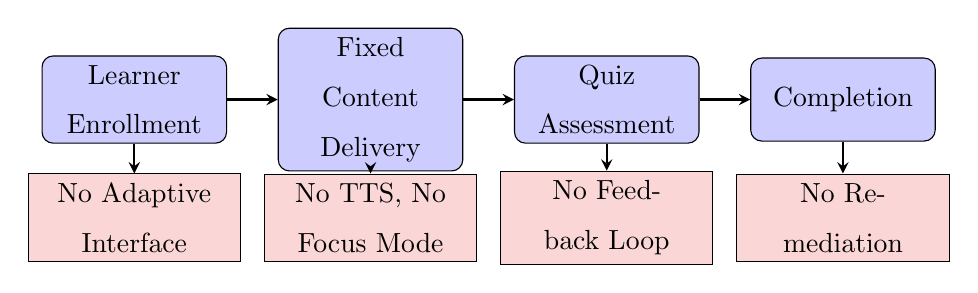
\begin{tikzpicture}[node distance=1.5cm, auto]
    \tikzstyle{block} = [rectangle, draw, fill=blue!20, text width=6em, text centered, rounded corners, minimum height=3em]
    \tikzstyle{problem} = [rectangle, draw, fill=red!20, text width=7em, text centered, minimum height=2.5em]
    \tikzstyle{arrow} = [thick,->,>=stealth]
    
    \node [block] (enroll) {Learner Enrollment};
    \node [block, right of=enroll, node distance=3cm] (content) {Fixed Content Delivery};
    \node [block, right of=content, node distance=3cm] (assess) {Quiz Assessment};
    \node [block, right of=assess, node distance=3cm] (complete) {Completion};
    
    \node [problem, below of=enroll, node distance=1.5cm] (p1) {No Adaptive Interface};
    \node [problem, below of=content, node distance=1.5cm] (p2) {No TTS, No Focus Mode};
    \node [problem, below of=assess, node distance=1.5cm] (p3) {No Feedback Loop};
    \node [problem, below of=complete, node distance=1.5cm] (p4) {No Remediation};
    
    \draw [arrow] (enroll) -- (content);
    \draw [arrow] (content) -- (assess);
    \draw [arrow] (assess) -- (complete);
    \draw [arrow] (enroll) -- (p1);
    \draw [arrow] (content) -- (p2);
    \draw [arrow] (assess) -- (p3);
    \draw [arrow] (complete) -- (p4);
\end{tikzpicture}
\caption{Current System Problem Analysis Diagram}
\label{fig:problem_analysis}
\end{figure}

\subsubsection{Detailed Problem Breakdown}

Figure~\ref{fig:problem_analysis} summarises that linear pipeline and the point at which each barrier arises. The problems identified in Chapter~1 are analysed here in greater technical depth:

\begin{enumerate}
    \item \textbf{Rigid Typography and Layout:} Standard LMS platforms use fixed CSS stylesheets that do not respond to individual user needs. Learners with Dyslexia require specific typographic conditions, including increased letter spacing (tracking) of at least 0.12em, line height of 1.5 to 1.8, and sans-serif fonts such as Atkinson Hyperlegible \cite{atkinson2021atkinson} designed to prevent letter confusion, such as differentiating 'b' from 'd' \cite{batanero2014accessibility}. Without these adjustments, reading velocity decreases and cognitive fatigue accelerates, leading to early lesson abandonment.
    \item \textbf{Cognitive Overload from Navigation:} Platforms like Moodle and Blackboard present deeply nested navigation menus (often three to four levels deep) combined with dense dashboard widgets showing calendars, announcements, grades, and messages simultaneously. For learners with ADHD \cite{barkley1997adhd}, this multi-stimulus environment triggers rapid attention fragmentation, making it difficult to sustain focus on a single learning objective. The absence of a distraction-free mode means learners must manually close or minimize interface elements.
    \item \textbf{Lack of Adaptive Remediation:} Current assessment systems grade quizzes and record scores but do not analyze performance patterns to generate corrective action. When a learner fails a prerequisite concept, the system does not automatically unlock remedial content or recommend revision. This linear progression model assumes uniform learner readiness, which is particularly detrimental for neurodivergent students who may require repeated exposure to foundational topics before advancing.
\end{enumerate}

\subsection{Requirement Analysis}

\subsubsection{Data Requirement}

The ACESS platform requires a robust relational data model to manage the complex relationships between users, courses, lessons, assessments, and accessibility preferences. The system must store and process the following categories of data:

\begin{itemize}
    \item \textbf{User Data:} Authentication credentials (email, password hash), profile information (name, avatar, role), and notification preferences. User data must be isolated by role with strict access controls.
    \item \textbf{Accessibility Data:} Per-user cognitive profile settings, including the active preset, font family and size, line-spacing multiplier, word spacing, background tint, theme, layout and structure mode, animation level, text-to-speech and caption toggles, and the executive-function supports (task checklist, visual schedule, step-by-step guidance, progress timeline, auto-save indicator). These settings must persist across sessions and apply globally. They are stored as a single JSON document on the user's profile row rather than as a wide table of columns, because the setting vocabulary is expected to change more often than the rest of the schema and because every consumer reads the whole object at once. Section~\ref{sec:data-dict} discusses the normalisation trade-off this represents.
    \item \textbf{Curriculum Data:} Hierarchical course structures (courses, chapters, lessons) with rich-text HTML content, video assets, transcripts, and metadata such as difficulty level, estimated duration, and prerequisite relationships that drive the adaptive engine.
    \item \textbf{Assessment Data:} Quiz configurations (time limits, pass thresholds, max attempts), question banks with multiple-choice and scenario formats, answer options with correctness flags, and learner attempt records including scores and answer selections.
    \item \textbf{Telemetry Data:} Granular engagement metrics including lesson view status, time spent per lesson (in seconds), enrollment status (active, completed, dropped), and quiz attempt history with pass/fail outcomes.
    \item \textbf{Content and Achievement Data:} Interactive activity configurations (flashcards, drag-and-drop, memory games, timelines), certificate records with unique reference codes, and badge/achievement definitions and user progress toward them.
    \item \textbf{Notification and Communication Data:} System-generated notifications triggered by enrollment, quiz attempts, lesson additions, and course publications, along with lesson-level threaded comments and contact form submissions.
\end{itemize}

The detailed database schema and data dictionary for these entities are presented in Section~\ref{sec:data-dict}.

\subsubsection{Functional Requirement}

Functional requirements define the explicit behaviors, processes, and services the system must execute. They are derived directly from the system's operational architecture and are categorized by user role.

\paragraph{Use Case Diagram}

\begin{figure}[H]
\centering
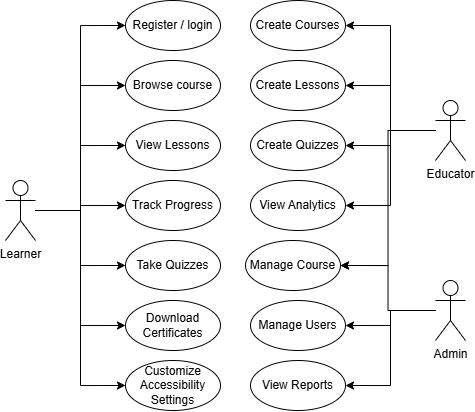
\includegraphics[width=0.8\textwidth,height=0.88\textheight,keepaspectratio]{Diagram/Figure 3.2 Use Case Diagram for ACESS Platform.png}
\caption{Use Case Diagram for ACESS Platform}
\label{fig:usecase_diagram}
\end{figure}

Figure \ref{fig:usecase_diagram} visually maps the interactions between the primary actors (Student, Educator, Admin) and the system's functional boundaries, which are explicitly detailed in the subsequent tables.

\paragraph{Learner Functions}

Table~\ref{tab:fr_student} lists the functional requirements of the learner module.

{
\renewcommand{\arraystretch}{1.2}
\footnotesize
\begin{longtable}{|>{\raggedright\arraybackslash\tabbreak}p{2.09cm}|>{\raggedright\arraybackslash\tabbreak}p{2.92cm}|>{\centering\arraybackslash\tabbreak}p{1.5cm}|>{\raggedright\arraybackslash\tabbreak}p{2.09cm}|>{\raggedright\arraybackslash\tabbreak}p{3.76cm}|}
\caption{Functional Requirements: Learner Module}
\label{tab:fr_student}\\
\hline
\textbf{Req ID} & \textbf{Description} & \textbf{Actor} & \textbf{Inputs} & \textbf{Outputs} \\ \hline \hline
\endfirsthead
\multicolumn{5}{l}{\footnotesize\itshape Table~\ref{tab:fr_student} continued from the previous page}\\
\hline
\textbf{Req ID} & \textbf{Description} & \textbf{Actor} & \textbf{Inputs} & \textbf{Outputs} \\ \hline \hline
\endhead
\hline
\multicolumn{5}{r}{\footnotesize\itshape continued on the next page}\\
\endfoot
\endlastfoot
FR-STU-01 & Registration and secure login. & Learner & Email, password & Supabase Auth session (JWT in an HTTP-only cookie), and a provisioning trigger creates the matching \tcode{users} and \tcode{user_profiles} rows with the role pinned to \tcode{learner}. \\ \hline
FR-STU-02 & Accessibility preset and setting selection. & Learner & Preset choice, or any individual setting & Preview of what will change, then an UPDATE of \tcode{user_profiles.accessibility_prefs}, after which the document root's \tcode{data-*} attributes and CSS custom properties change immediately. \\ \hline
FR-STU-03 & Course discovery and enrolment. & Learner & \tcode{course_id} selection & INSERT into \tcode{enrollments} under RLS, and a notification trigger informs the educator. \\ \hline
FR-STU-04 & Lesson viewing with adaptive presentation. & Learner & Navigation to \tcode{/learner/lesson/[id]} & Renders sanitised HTML at the profile's reading measure, layout mode and typography, optionally hiding navigation chrome. \\ \hline
FR-STU-05 & In-video questions. & Learner & Playback reaching a stored timestamp & Pauses the YouTube player and overlays the question from \tcode{video_questions}. \\ \hline
FR-STU-06 & Quiz attempt. & Learner & Selected option identifiers & Calls a database function that grades server-side and writes \tcode{quiz_attempts} and \tcode{quiz_answers}. The client never receives the answer key before submission. \\ \hline
FR-STU-07 & Automated progress telemetry. & Learner & Dwell time on the lesson route & UPDATEs \tcode{lesson_progress.time_spent_learning}, \tcode{view_count} and the viewed/completed flags. \\ \hline
FR-STU-08 & Achievement earning. & Learner & Course progress reaching a threshold & A database function derives completion and inserts the earned \tcode{user_achievements} rows. The client cannot award a badge directly. \\ \hline
FR-STU-09 & Certificate claim and download. & Learner & Course completion & A database function gates the claim, a reference code and public verification URL are issued, and the PDF is rendered client-side with jsPDF. \\ \hline
FR-STU-10 & Text-to-speech playback. & Learner & Press of the Listen control & Speech synthesis of the lesson text at the learner's chosen rate. Never starts automatically. \\ \hline
FR-STU-11 & Adaptive recommendations. & Learner & Quiz results, viewing history, favourites & Reads \tcode{recommendations} and displays revision, next-lesson, near-completion and cross-course suggestions with the reason for each. \\ \hline
FR-STU-12 & Favourites and lesson discussion. & Learner & Save action, comment text & INSERT into \tcode{course_favorites}, and a threaded INSERT into \tcode{lesson_comments}. \\ \hline
FR-STU-13 & AI lesson assistant. & Learner & Question about the open lesson & A model-generated answer scoped to that lesson's content, plus a cached plain-language summary in \tcode{lesson_ai_summaries}. \\ \hline
FR-STU-14 & Interface language switch. & Learner & English or Bahasa Melayu & Interface strings re-render immediately, and the choice persists to \tcode{user_profiles.preferred_language}. \\ \hline
\end{longtable}
}

\paragraph{Educator Functions}

Table~\ref{tab:fr_educator} lists the functional requirements of the educator module. Requirement FR-EDU-05 is the one with no counterpart in the platforms surveyed in Chapter~2, and its design is set out in Section~\ref{sec:a11y-audit}.

{
\renewcommand{\arraystretch}{1.2}
\footnotesize
\begin{longtable}{|>{\raggedright\arraybackslash\tabbreak}p{2.09cm}|>{\raggedright\arraybackslash\tabbreak}p{2.92cm}|>{\centering\arraybackslash\tabbreak}p{1.5cm}|>{\raggedright\arraybackslash\tabbreak}p{2.09cm}|>{\raggedright\arraybackslash\tabbreak}p{3.76cm}|}
\caption{Functional Requirements: Educator Module}
\label{tab:fr_educator}\\
\hline
\textbf{Req ID} & \textbf{Description} & \textbf{Actor} & \textbf{Inputs} & \textbf{Outputs} \\ \hline \hline
\endfirsthead
\multicolumn{5}{l}{\footnotesize\itshape Table~\ref{tab:fr_educator} continued from the previous page}\\
\hline
\textbf{Req ID} & \textbf{Description} & \textbf{Actor} & \textbf{Inputs} & \textbf{Outputs} \\ \hline \hline
\endhead
\hline
\multicolumn{5}{r}{\footnotesize\itshape continued on the next page}\\
\endfoot
\endlastfoot
FR-EDU-01 & Course creation and editing. & Educator & Title, metadata, difficulty, accessibility focus profile & INSERT/UPDATE on \tcode{courses}, restricted by RLS to rows the educator created. \\ \hline
FR-EDU-02 & Lesson authoring. & Educator & Rich text, headings, images, tables, links & Sanitised HTML written to \tcode{lessons.content_html}, with a snapshot appended to \tcode{lesson_versions}. \\ \hline
FR-EDU-03 & Quiz and activity creation. & Educator & Question text, options, correct-option flag, activity configuration & Populates \tcode{quiz_questions} and \tcode{quiz_options}, and activity payloads are stored as typed JSON in \tcode{lesson_interactive_content}. \\ \hline
FR-EDU-04 & Asset management. & Educator & Image, document and media files & Uploads to the \tcode{course-assets} storage bucket and records the reference in \tcode{media_assets}. Instructional video is embedded from an external host rather than uploaded. \\ \hline
FR-EDU-05 & Accessibility compliance check. & Educator & The lesson draft currently open, plus the course's focus profile & A score out of 100, a pass/fail list of the applicable standards, the source of each rule, the editor tab that fixes it, and a one-click fix where one exists. Re-evaluated on every keystroke against unsaved form state. \\ \hline
FR-EDU-06 & Student monitoring and analytics. & Educator & Course or student selection & Recharts visualisations aggregating \tcode{lesson_progress} and \tcode{quiz_attempts}, with at-risk flagging. \\ \hline
FR-EDU-07 & Achievement and milestone configuration. & Educator & Requirement type and threshold & Rows in \tcode{course_achievements} and \tcode{course_milestones}. \\ \hline
FR-EDU-08 & Certificate issue and revocation. & Educator & Learner selection, revocation reason & INSERT or UPDATE on \tcode{certificates}. A revoked certificate keeps its row and reference code so that verification reports the revocation rather than a missing record. \\ \hline
FR-EDU-09 & Preview as learner. & Educator & Course or lesson selection & Renders the learner-facing view without creating an enrolment or progress record. \\ \hline
FR-EDU-10 & Lesson version history. & Educator & Version selection & Restores a previous \tcode{content_html} snapshot from \tcode{lesson_versions}. \\ \hline
\end{longtable}
}

\paragraph{Administrator Functions}

Table~\ref{tab:fr_admin} lists the functional requirements of the administrator module.

{
\renewcommand{\arraystretch}{1.2}
\footnotesize
\begin{longtable}{|>{\raggedright\arraybackslash\tabbreak}p{2.09cm}|>{\raggedright\arraybackslash\tabbreak}p{2.92cm}|>{\centering\arraybackslash\tabbreak}p{1.5cm}|>{\raggedright\arraybackslash\tabbreak}p{2.09cm}|>{\raggedright\arraybackslash\tabbreak}p{3.76cm}|}
\caption{Functional Requirements: Administrator Module}
\label{tab:fr_admin}\\
\hline
\textbf{Req ID} & \textbf{Description} & \textbf{Actor} & \textbf{Inputs} & \textbf{Outputs} \\ \hline \hline
\endfirsthead
\multicolumn{5}{l}{\footnotesize\itshape Table~\ref{tab:fr_admin} continued from the previous page}\\
\hline
\textbf{Req ID} & \textbf{Description} & \textbf{Actor} & \textbf{Inputs} & \textbf{Outputs} \\ \hline \hline
\endhead
\hline
\multicolumn{5}{r}{\footnotesize\itshape continued on the next page}\\
\endfoot
\endlastfoot
FR-ADM-01 & User role management. & Admin & Target user, new role & A service-role API route UPDATEs \tcode{users.role} \emph{and} the corresponding authentication metadata, so that routing and database policy agree. A guard trigger blocks any attempt to change the same columns from a normal session. \\ \hline
FR-ADM-02 & Course moderation. & Admin & Approve or reject & UPDATEs \tcode{courses.status} from \tcode{pending_review} to \tcode{published} or back to \tcode{draft}, and a notification trigger informs the educator. \\ \hline
FR-ADM-03 & Educator application review. & Admin & Application decision, reviewer notes & UPDATEs \tcode{instructor_applications}. Approval promotes the applicant to \tcode{educator} in both the users table and the authentication metadata. \\ \hline
FR-ADM-04 & System course creation. & Admin & Course metadata & Creates a course flagged \tcode{system_course = true} and \tcode{managed_by_admin = true}, which the learner catalogue presents as an official course. \\ \hline
FR-ADM-05 & Platform analytics. & Admin & Date-range selection & Aggregates registrations, enrolments, completion, learning time, and accessibility adaptation and preset-adoption counts drawn from \tcode{adaptive_interactions}. \\ \hline
FR-ADM-06 & Report generation. & Admin & Report type, date range & A rendered PDF report, generated client-side with jsPDF, covering platform, course, learner and content-coverage views. \\ \hline
FR-ADM-07 & Certificate oversight. & Admin & Search or filter & Read access across all issued certificates, with revocation status. \\ \hline
FR-ADM-08 & Enquiry handling. & Admin & Message status change & UPDATEs \tcode{contact_messages.status} across the unread, read and replied states. \\ \hline
\end{longtable}
}

\subsubsection{Non-Functional Requirement}

Non-functional requirements (NFRs) specify the critical quality attributes and systemic constraints that govern the operation of the ACESS platform.

\paragraph{Performance}
\begin{itemize}
    \item \textbf{Page Response Time:} Client-side route transitions should complete within \textbf{300\,ms} so that navigation does not itself become a source of cognitive disruption.
    \item \textbf{Course Loading:} Initial course data fetches should resolve within \textbf{800\,ms} on a broadband connection.
    \item \textbf{Setting Application Latency:} A change to any accessibility setting must be visible \textbf{without a page reload}. This is the strictest performance requirement in the system, because a learner adjusting spacing or size is engaged in a feedback loop and cannot evaluate the change if it does not appear immediately. It is met by writing CSS custom properties and \tcode{data-*} attributes on the document root rather than by re-rendering the component tree.
    \item \textbf{Video Loading:} Instructional video is embedded from an external host rather than served from platform storage. Playback start therefore depends on that host, and no delivery target is asserted for it here.
    \item \textbf{Concurrency:} The managed PostgreSQL instance uses connection pooling supplied by the platform. No concurrent-user figure is claimed, because no load test has been carried out on this project. Establishing one is identified in Chapter~4 as future work.
\end{itemize}

\paragraph{Security}
\begin{itemize}
    \item \textbf{Authentication:} All user sessions are secured with JSON Web Tokens managed by Supabase Auth \cite{supabase_auth} and carried in HTTP-only cookies, with a 15-minute inactivity timeout that warns 30 seconds before it takes effect.
    \item \textbf{Authorisation (RBAC):} The request interceptor at \tcode{src/proxy.ts} gates every non-public route on the role claim in the session token. This layer is deliberately treated as a \emph{routing} control, not as the security boundary: the authoritative check is made again inside the database by RLS policies that read \tcode{public.users.role}, and inside privileged API routes that re-verify the caller under the service role. A forged token therefore obtains a user-interface shell and nothing behind it. Section~\ref{sec:phys-db} documents this two-layer arrangement and its rationale.
    \item \textbf{Database Protection:} Row-Level Security must be enabled on \textbf{every} table in the application schema (currently 36 of 36, carrying 88 policies), so that isolation holds at the storage layer regardless of which client issues the query. This is verified by an automated probe (\tcode{npm run verify:rls}) rather than asserted.
    \item \textbf{Privilege Guards:} Three database trigger functions prevent a learner from forging an outcome even with a valid session: one blocks self-promotion by rejecting a client attempt to change a privileged account column, another blocks declaring a course complete outside the normal completion process, and a third blocks writing a quiz score directly instead of through the grading function. They exempt only the service role and the platform's own trusted derivation logic.
    \item \textbf{Input Handling:} Rich-text lesson content is sanitised with DOMPurify \cite{dompurify} before rendering, which is the platform's principal cross-site-scripting control. All database access goes through parameterised PostgREST or \tcode{pg} queries, so string-concatenated SQL does not occur. Field-level validation is performed in the form components and enforced a second time by \texttt{CHECK} constraints in the schema. A single shared schema-validation library is \emph{not} currently used, and adopting one is listed as future work in Section~\ref{sec:design-limitations}.
\end{itemize}

\paragraph{Accessibility}
\begin{itemize}
    \item \textbf{WCAG Target:} The platform \emph{targets} \textbf{WCAG 2.2 Level AA} \cite{wcag22} together with four Level AAA criteria (1.4.8, 2.2.6, 2.3.3, 3.2.5). Body-text contrast must meet or exceed 4.5:1. Conformance is a target rather than an audited result, discussed further in Section~\ref{sec:a11y-design}.
    \item \textbf{Dyslexia Support:} The system must provide the Atkinson Hyperlegible \cite{atkinson2021atkinson} and OpenDyslexic \cite{opendyslexic} typefaces, a line-spacing multiplier adjustable from 1.0 to 3.0, and word spacing reaching at least the WCAG 1.4.12 floor of 0.16\,em at a setting the learner can actually reach on the slider.
    \item \textbf{Reading Measure:} Lesson text must be bounded by a measure expressed in character units, so that line length remains within the 50--80 character band as font size changes: 72 characters by default, 62 under the Dyslexia preset, 66 under the ADHD preset. The bound must hold when navigation chrome is hidden, not be released by it.
    \item \textbf{ADHD and Autism Support:} A single animation-level setting must reduce or remove motion across the interface. No media may autoplay, and text-to-speech must never begin without an explicit action.
    \item \textbf{Screen Reader Compatibility:} Custom components must expose the appropriate WAI-ARIA states, navigation must be built from real links rather than click handlers, and every interactive activity must be operable from the keyboard. It must be recorded, however, that no assistive-technology testing has yet been performed against this build. This requirement is therefore currently met by construction and code review only.
\end{itemize}

\paragraph{Usability}
\begin{itemize}
    \item \textbf{Consistent Navigation:} The primary navigational architecture must remain structurally identical across all modules to ensure predictability for Autistic learners.
    \item \textbf{Error Prevention:} Destructive actions (e.g., an Educator deleting a course) must require a confirmed multi-step verification modal to prevent accidental data loss.
\end{itemize}

\paragraph{Reliability}
\begin{itemize}
    \item \textbf{Data Integrity:} The database schema must strictly enforce foreign key constraints with cascade deletes where appropriate to prevent orphaned records, such as a lesson progress record existing without a valid enrollment.
    \item \textbf{Backup and Reproducibility:} The hosted Supabase project relies on the provider's managed backup facility. Independently of that, the entire schema must be reconstructible from version-controlled migrations, and the demonstration dataset from a deterministic seed script, so that a complete working database can be rebuilt from the repository alone. This is exercised routinely (\tcode{npm run db:rebuild}) and is what makes the figures in Chapter~4 reproducible.
\end{itemize}

\paragraph{Maintainability and Scalability}
\begin{itemize}
    \item \textbf{Modular Architecture:} The codebase must adhere to strict separation of concerns, decoupling the data-fetching logic (Server Components) from the interactive accessibility logic (Client Components).
    \item \textbf{Database Normalization:} The schema must adhere to the Third Normal Form (3NF) to eliminate data redundancy, ensuring the database scales efficiently as course and user volume increases.
\end{itemize}

\subsubsection{Others Requirement}

The software and hardware tools selected for the ACESS platform, as listed in Chapter 2, Section 2.4, are justified by the following architectural considerations:

\begin{itemize}
    \item \textbf{Next.js 16 and React \cite{nextjs_ssr}:} Server-side rendering reduces the initial JavaScript payload, which matters for the rapid page loads that prevent cognitive drop-off for ADHD learners. The App Router's request interceptor (\tcode{src/proxy.ts}) performs role-based route gating before a protected page is rendered \cite{nextjs_middleware}.
    \item \textbf{Supabase with PostgreSQL \cite{supabase_docs}:} Row-Level Security provides data isolation \cite{supabase_rls} at the database level rather than relying solely on application-layer guards, ensuring that cognitive telemetry and assessment data remain cryptographically isolated per user.
    \item \textbf{Tailwind CSS v4 \cite{tailwind_docs}:} Just-in-Time compilation enables dynamic CSS variable injection, allowing instantaneous theme and typography switching without JavaScript re-evaluation, which is essential for real-time accessibility adjustments.
    \item \textbf{TypeScript \cite{typescript_docs}:} Static typing across the full stack reduces runtime errors in critical paths such as quiz scoring and accessibility profile application, where a type mismatch could result in incorrect interface rendering.
    \item \textbf{Vercel \cite{vercel_docs}:} Serverless edge deployment provides global low-latency access to the platform, which is particularly important for learners whose cognitive focus may be disrupted by slow page transitions.
\end{itemize}

\subsection{System Architecture}

The ACESS platform employs a modern, decoupled client-server architecture, leveraging edge computing paradigms to maximize performance and security.

\subsubsection{Context Diagram}
The Context Diagram establishes the highest-level view of the system, illustrating the boundaries of the ACESS platform and its interactions with external entities.

\begin{figure}[H]
\centering
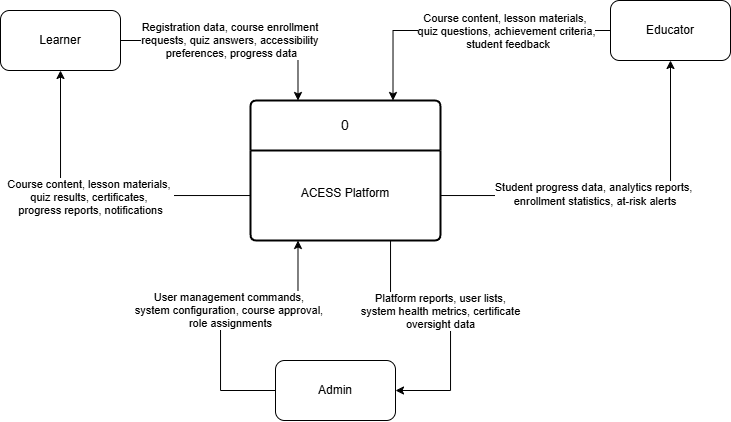
\includegraphics[width=0.8\textwidth,height=0.88\textheight,keepaspectratio]{Diagram/Figure 3.3 Context Diagram.png}
\caption{Context Diagram}
\label{fig:context_diagram}
\end{figure}

As depicted in Figure~\ref{fig:context_diagram}, the ACESS system acts as the central processing hub. The primary external entities are the Learner (who consumes content and generates engagement telemetry), the Educator (who authors content and configures assessments), and the Administrator (who governs system integrity). Four external services sit on the system boundary:

\begin{itemize}
    \item an SMTP mail provider for password-recovery and notification messages
    \item an external video host, from which instructional video is embedded rather than uploaded
    \item the Gemini generative-model service, used only for the optional lesson summary and lesson assistant
    \item the browser's own Web Speech synthesis engine \cite{webspeech_api}, which performs text-to-speech locally on the learner's device rather than through a network service
\end{itemize}

That last choice is deliberate: it keeps read-aloud free of per-request cost and keeps lesson text from leaving the device in order to be spoken.

\subsubsection{System Architecture Diagram}

\begin{figure}[H]
\centering
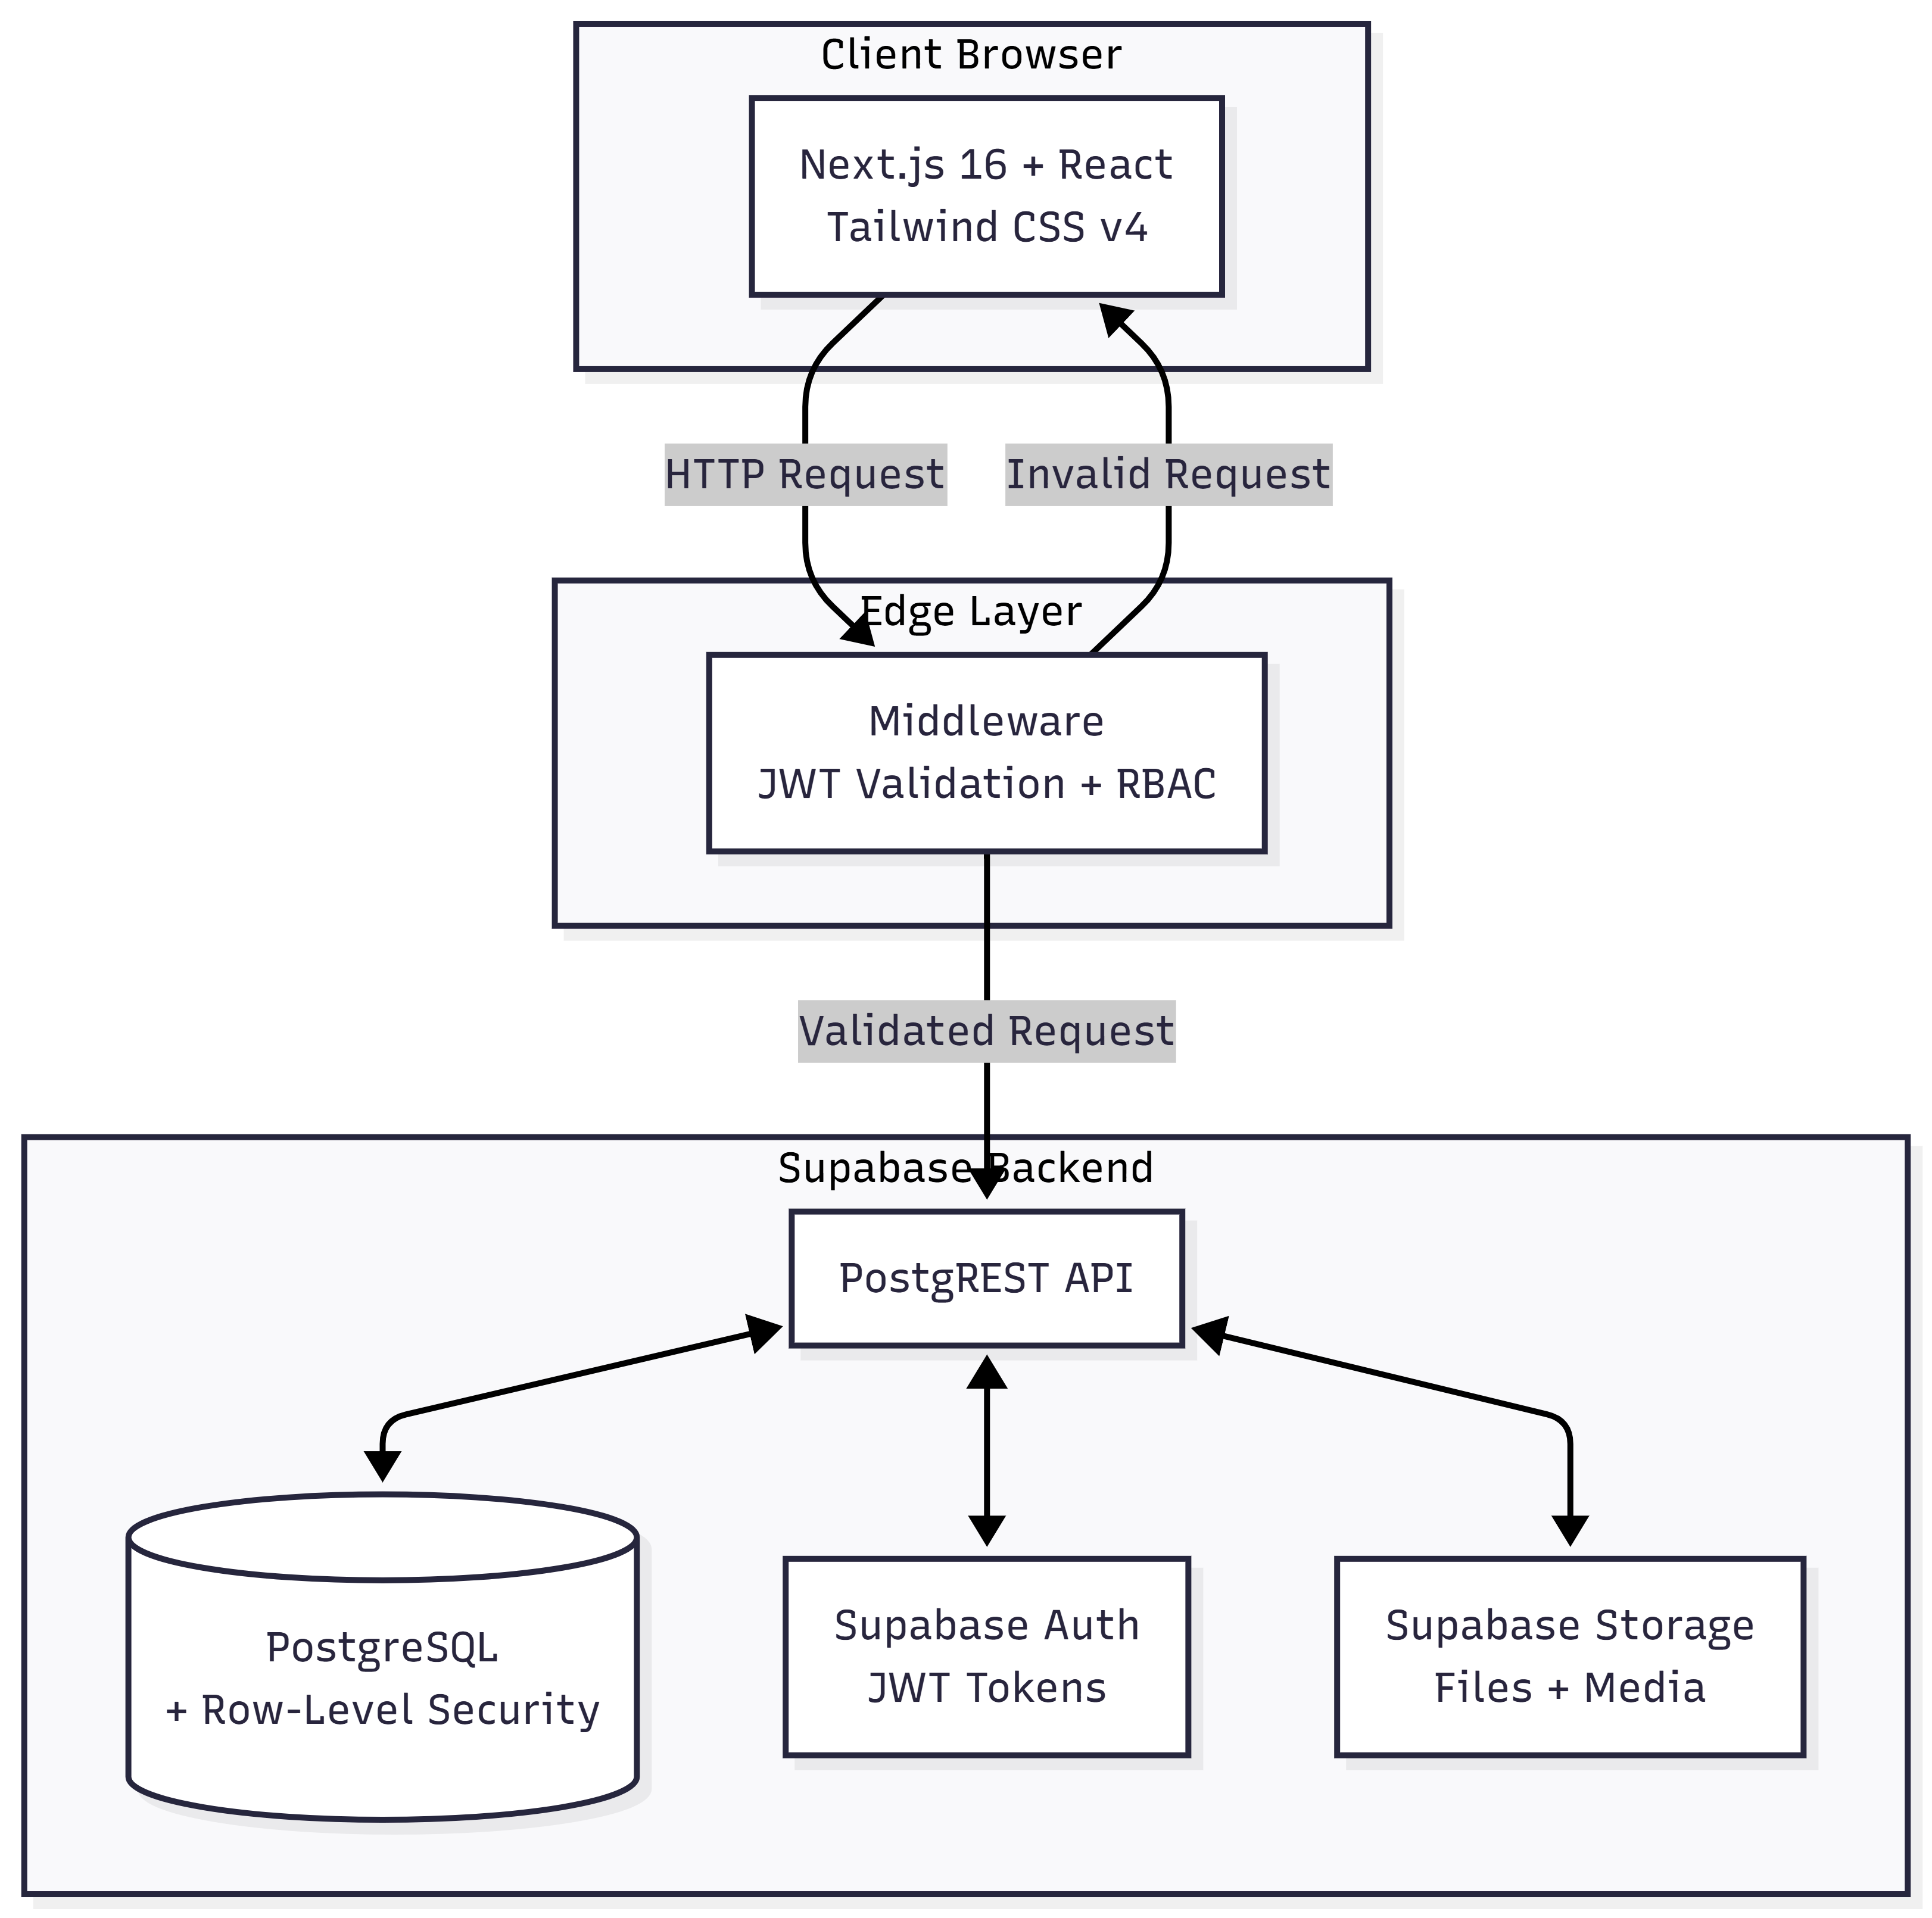
\includegraphics[width=0.8\textwidth,height=0.88\textheight,keepaspectratio]{Diagram/Figure 3.4 System Architecture Diagram.png}
\caption{System Architecture Diagram}
\label{fig:system_architecture}
\end{figure}

Figure \ref{fig:system_architecture} details the three-tier decoupled architecture:
\begin{itemize}
    \item \textbf{Frontend Architecture (Next.js 16 and React):} The presentation layer is built on the Next.js App Router. It utilizes React Server Components to execute data fetching securely on the server, drastically reducing the JavaScript payload delivered to the client. This is crucial for rapid page loads, preventing cognitive drop-off for ADHD learners. Client components are restricted to highly interactive elements, such as the rich-text editor and interactive quiz interfaces. The UI is styled utilizing Tailwind CSS v4, which enables the dynamic injection of CSS variables for accessibility toggling.
    \item \textbf{Request Interception and Authentication Layer:} A Next.js request interceptor (\tcode{src/proxy.ts}) runs before every non-public route. It validates the session cookie with Supabase Auth, rejects suspended or deleted accounts, and gates the \tcode{/learner}, \tcode{/educator} and \tcode{/admin} prefixes on the role claim, redirecting unauthorised attempts before the page is rendered. It reads the role from the session token rather than the database, deliberately, to avoid a database round trip on every request. The authoritative role check is repeated in the database and in privileged API routes, so this layer decides \emph{which shell a user sees}, not \emph{which rows they may touch}.
    \item \textbf{Backend and Database Architecture (Supabase):} Supabase provides a managed PostgreSQL 17 database exposed over HTTP by PostgREST \cite{postgrest_docs}. Security does not rest on the application layer: 88 Row-Level Security policies across all 36 tables are written into the schema itself, three guard triggers prevent privilege and outcome forgery, and the two operations that must not be client-decided (quiz grading and course completion) are implemented as \texttt{SECURITY DEFINER} database functions rather than as client logic.
    \item \textbf{Storage Architecture:} Three Supabase Storage buckets hold unstructured assets: \tcode{course-assets} for lesson media and course thumbnails, \tcode{certificates} for educator-uploaded custom certificates, and \tcode{avatars} for profile pictures. All three are public-read, because the application distributes public URLs that are rendered directly in the page. Write access is restricted by policy, and a learner may only write inside a folder named for their own user identifier. Instructional video is \emph{not} stored in these buckets. It is embedded from an external host, and completion certificates are generated in the browser at download time rather than persisted as files.
\end{itemize}

\subsubsection{Deployment Diagram}

\begin{figure}[H]
\centering
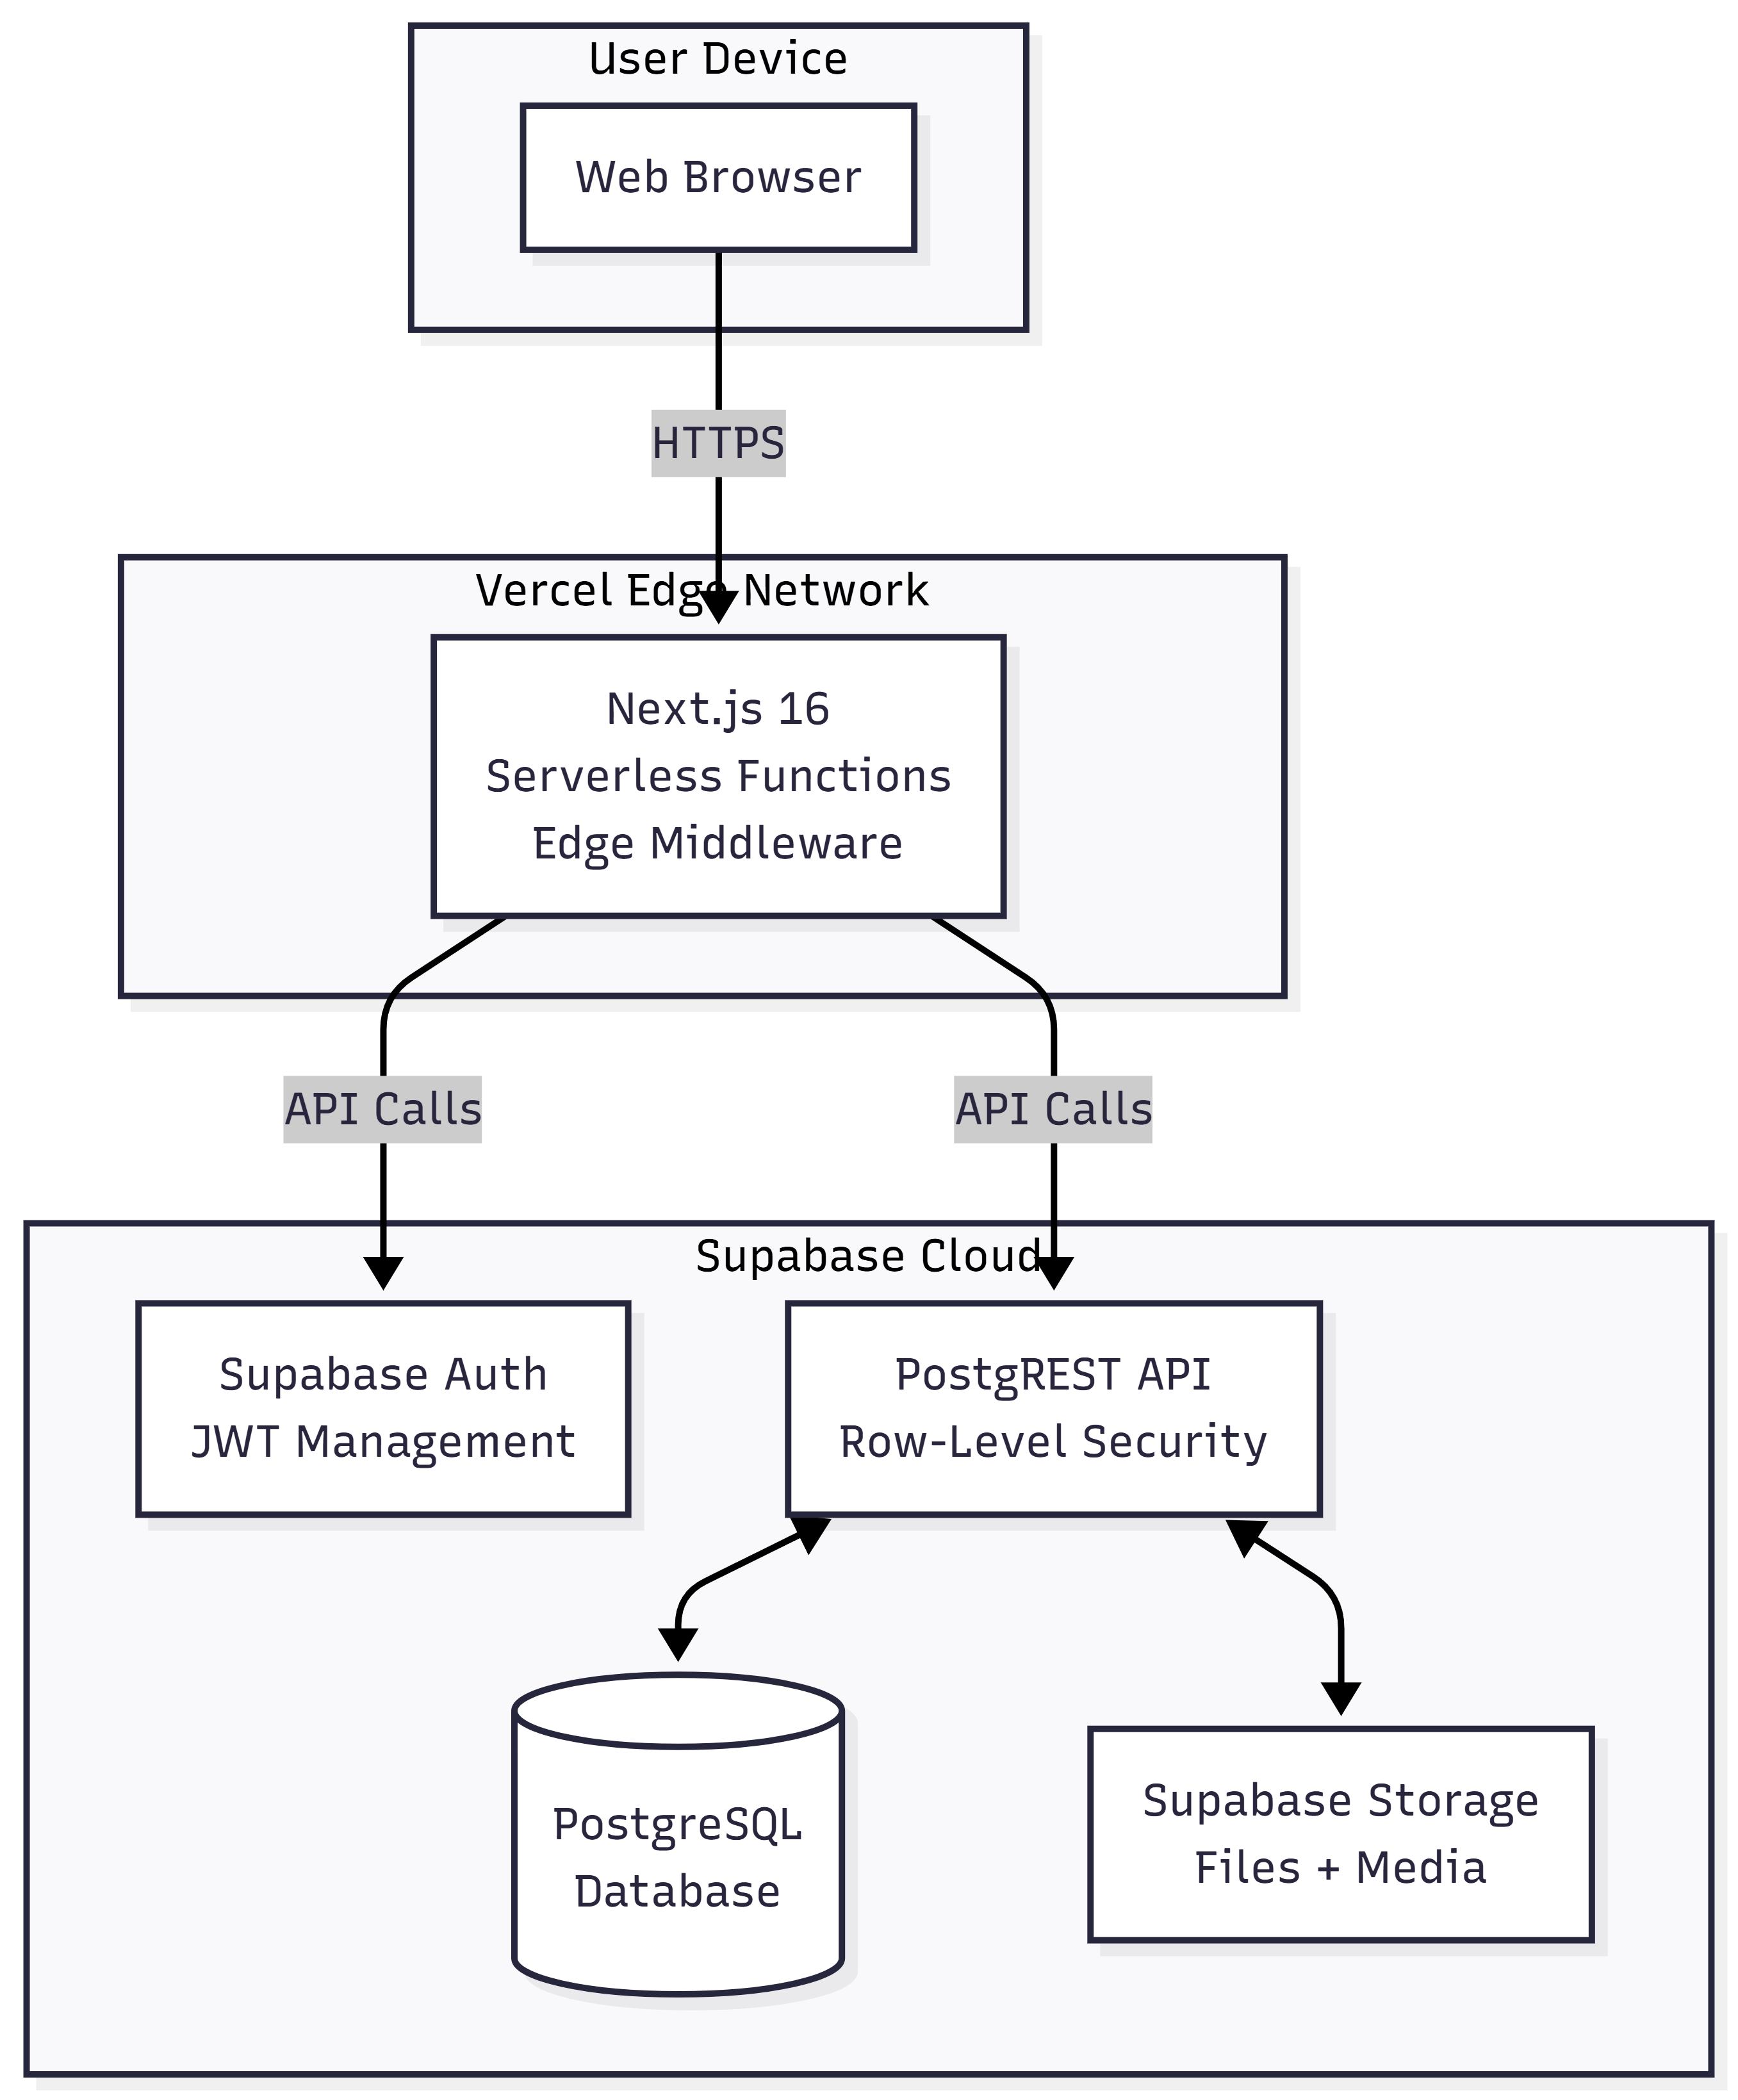
\includegraphics[width=0.8\textwidth,height=0.88\textheight,keepaspectratio]{Diagram/Figure 3.5 Deployment Diagram.png}
\caption{Deployment Diagram}
\label{fig:deployment_diagram}
\end{figure}

The Deployment Diagram (Figure~\ref{fig:deployment_diagram}) illustrates the physical distribution of the system components. The Next.js application is deployed to Vercel's serverless platform \cite{vercel_docs}, which builds from the GitHub repository on each push to the release branch. The Supabase backend operates on managed cloud infrastructure, exposing the schema as a REST interface through PostgREST \cite{postgrest_docs}, which both the browser client (under the anonymous key, and therefore under RLS) and the server-side API routes consume. A small number of routes (account provisioning, role changes, recommendation generation and certificate issue) use the service-role key and therefore bypass RLS by design. These run only on the server and are the reason those operations are implemented as API routes rather than as client calls.

A second, complete deployment of the same system runs locally under Docker for development, comprising the PostgreSQL database, the authentication service, PostgREST, the storage service and the Supabase Studio console. Because the schema is defined entirely by version-controlled migrations, this local stack is rebuilt from empty on demand, which is what makes the database evidence presented in Section~\ref{sec:phys-db} reproducible rather than a description of a single mutable instance.

\subsection{Module Design}

The system is logically partitioned into discrete, highly cohesive modules to facilitate maintainability.

\begin{itemize}
    \item \textbf{Student Module:} Encapsulates all logic related to course discovery, enrollment, lesson consumption, and quiz execution.
    \item \textbf{Educator Module:} Manages the creation pipeline. Handles the rich-text editor state, quiz generation, and the uploading of media assets to storage.
    \item \textbf{Admin Module:} Provides a high-level oversight interface for user management, role reassignment, and global accessibility preset configurations.
    \item \textbf{Accessibility Module:} A globally available React context provider that loads the learner's stored preferences, resolves conflicts between them, and writes the result to the document root as \tcode{data-*} attributes and CSS custom properties, from which the stylesheet derives typography, palette, reading measure and motion behaviour.
    \item \textbf{Accessibility Compliance Module:} A pure, synchronous auditing engine shared by two surfaces: the lesson editor, which re-runs it against unsaved form state on every edit, and the course-level report, which runs the same rules against rows read from the database. Because it is deterministic and side-effect free, both surfaces necessarily agree.
    \item \textbf{Interactive Activity Module:} Governs five activity types together with in-video questions and embedded H5P content. Multiple-choice assessment is handled separately, and is graded inside the database rather than in this module.
    \item \textbf{Analytics Module:} Aggregates lesson progress, quiz attempts and accessibility adaptation events into visualisations, giving educators cohort-level insight and administrators platform-level insight, including which accessibility features are actually being used.
\end{itemize}

\subsection{Summary}

This chapter analyzed the engineering specifications required to build the ACESS platform. It began with a detailed problem analysis of existing educational systems, followed by a comprehensive requirements analysis covering data, functional, non-functional, and other requirements. The system architecture was presented through Context, Architecture, and Deployment diagrams, and the modular decomposition of the system was described. The subsequent chapter will translate these requirements into concrete database schemas and interface designs.

%==========================================================%

\newpage
\vfill \null
\thispagestyle{empty}
\begin{center}
\section{SYSTEM DESIGN}
\end{center}
\vspace{2cm}

\subsection{Introduction}

This chapter translates the requirements established in the previous chapter into concrete engineering design. It is organised in the order the writing guide prescribes. High-Level Design comes first, covering behavioural and interaction diagrams, user interface design, and the conceptual and logical database model. The accessibility design that is this project's substantive contribution follows, then the data dictionary, and finally Detailed Design, which covers software components and the physical database implementation.

Two things about this chapter differ from a conventional design chapter, and both are deliberate. First, the figures are evidence rather than illustration. The interface figures are screenshots of the running system taken against a database that can be rebuilt from the repository, and the Entity Relationship Diagrams are generated from that database's own catalogue by a script in the repository. A design chapter that documents an intended system rather than the built one is of no use in verifying either. The previous revision of this report had drifted in exactly that way, documenting six database tables that no longer exist and one accessibility settings table that was never read by any code path.

Second, Section~\ref{sec:a11y-design} states what the accessibility implementation does \emph{and} what it does not do. A design chapter for an accessibility project that lists only successes would be the same failure as an inert setting that looks like it works.

\subsection{High-Level Design}

\subsubsection{Behavioral Design (Activity Diagrams)}

Activity diagrams model the workflow of the system, illustrating the procedural logic executed by the different actors.

\paragraph{Student Activity Diagram}

\begin{figure}[H]
\centering
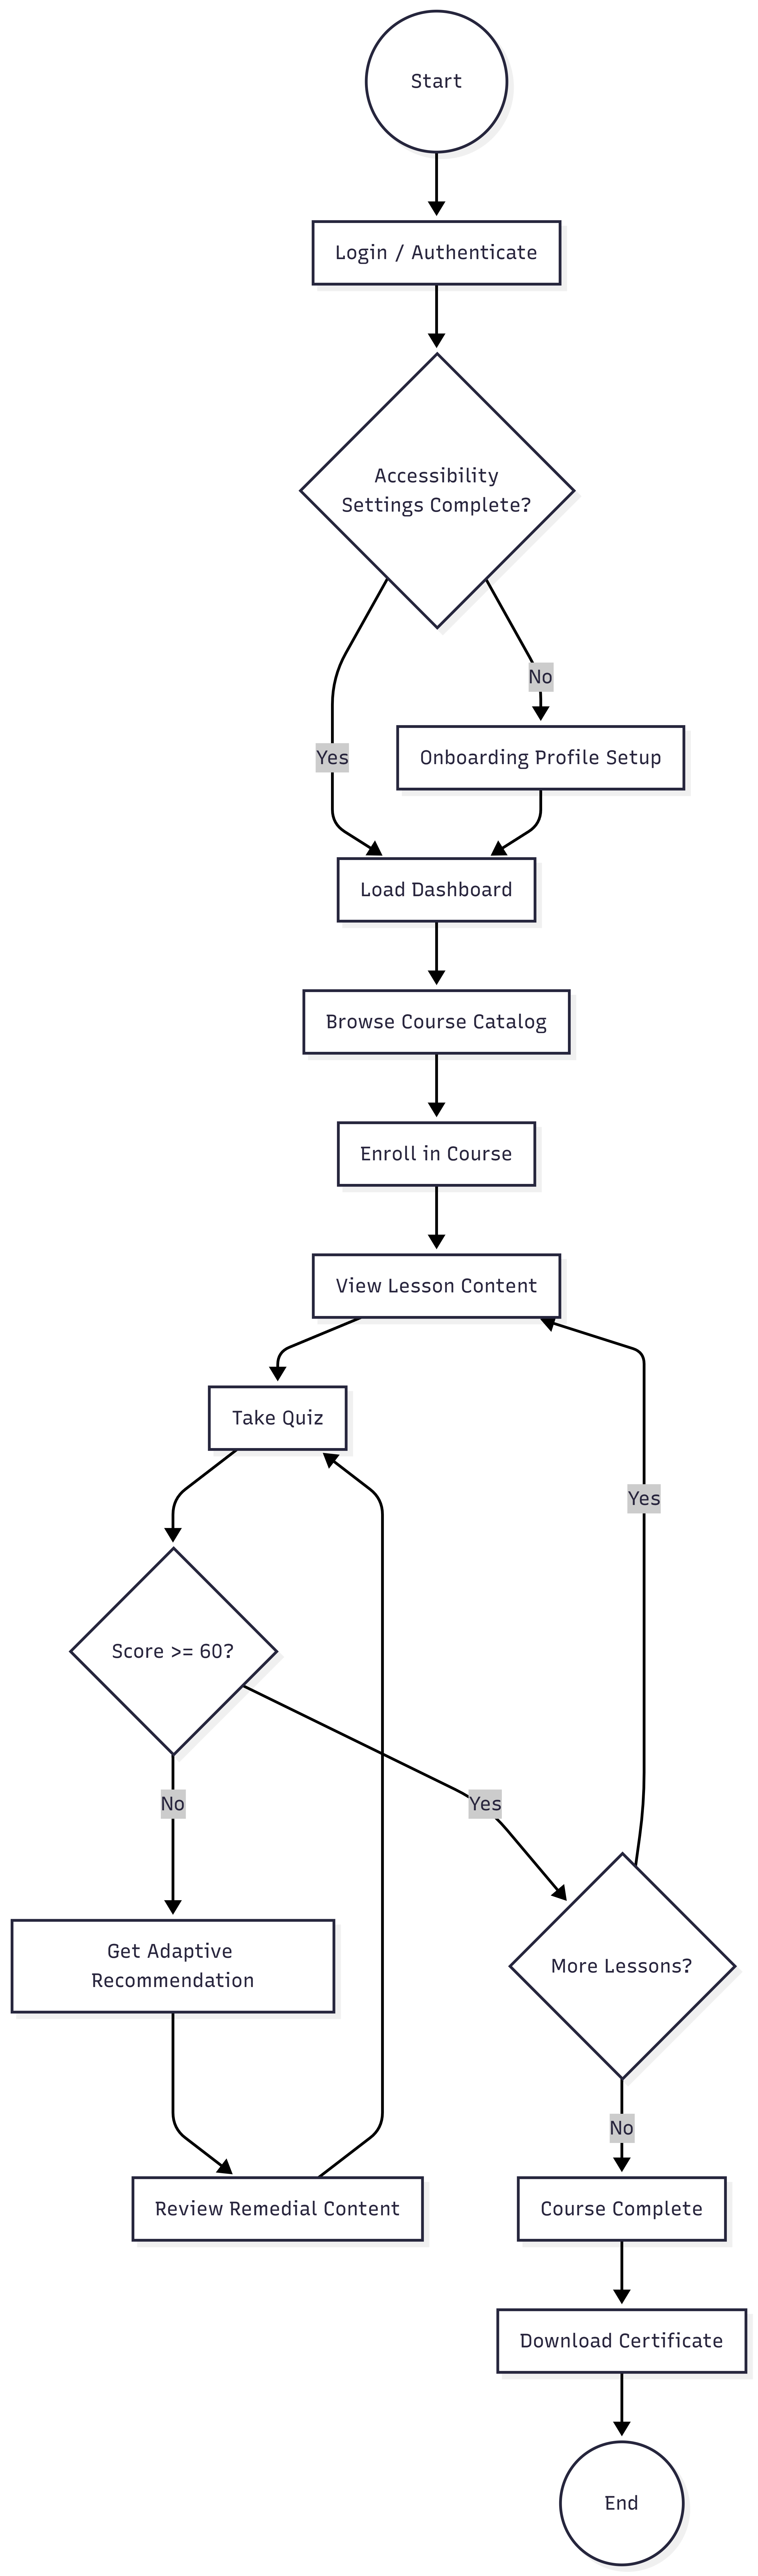
\includegraphics[width=0.55\textwidth,height=0.88\textheight,keepaspectratio]{Diagram/Figure 4.1 Student Activity Diagram.png}
\caption{Student Activity Diagram}
\label{fig:act_student}
\end{figure}

As shown in Figure~\ref{fig:act_student}, the learner workflow has one structural feature that distinguishes it from a conventional course flow. On authentication the route interceptor resolves the role and admits the learner shell. The accessibility provider then loads the learner's stored accessibility preferences and writes the resolved settings onto the document root before the first lesson is rendered, so a learner never sees an unstyled pass followed by a correction. A learner with no stored preferences is offered onboarding, but is not blocked by it. An accessibility profile is an aid, not a gate.

The core loop is browsing the catalogue, enrolling in a course, and working through its lessons in order, with progress updated as each lesson is opened and completed. The branch of interest occurs after assessment. The attempt is graded by the database, not the client. If the resulting score falls below the quiz's pass threshold, the recommendation engine records a revision-tier recommendation naming the lesson and the score that triggered it. That recommendation is surfaced prominently, but it does not lock the learner out of the next lesson. Forcing remediation would convert a support into a punishment, which for a learner already struggling is the wrong intervention.

\paragraph{Educator Activity Diagram}

\begin{figure}[H]
\centering
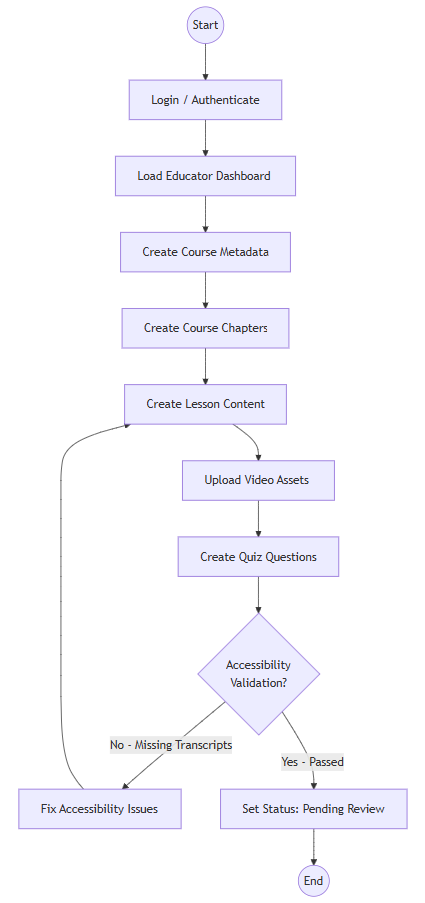
\includegraphics[width=0.75\textwidth,height=0.88\textheight,keepaspectratio]{Diagram/Figure 4.2 Educator Activity Diagram.png}
\caption{Educator Activity Diagram}
\label{fig:act_educator}
\end{figure}

Figure~\ref{fig:act_educator} maps the educator's authoring workflow. The process begins with course metadata and, optionally, chapter structure, and includes one decision with consequences throughout the rest of the flow: the course's \emph{primary accessibility focus}. That choice selects which rule set the compliance auditor will apply to every lesson in the course, so an educator writing for dyslexic readers is checked on sentence length and readability while one writing for autistic learners is checked on figurative language and stated objectives.

The educator then enters a content loop: drafting lesson text, embedding media, building activities and writing quiz questions. The auditor re-evaluates the draft continuously against unsaved editor state, so the accessibility score in the editor header moves as the lesson is written rather than appearing at the end. When the educator submits the course, its status moves to pending review for administrator moderation. The accessibility check is \emph{not} a gate in the publication path: a lesson with unmet standards can still be saved and published, and the panel says so explicitly. The reasoning is given in Section~\ref{sec:a11y-audit}.

\paragraph{Administrator Activity Diagram}

\begin{figure}[H]
\centering
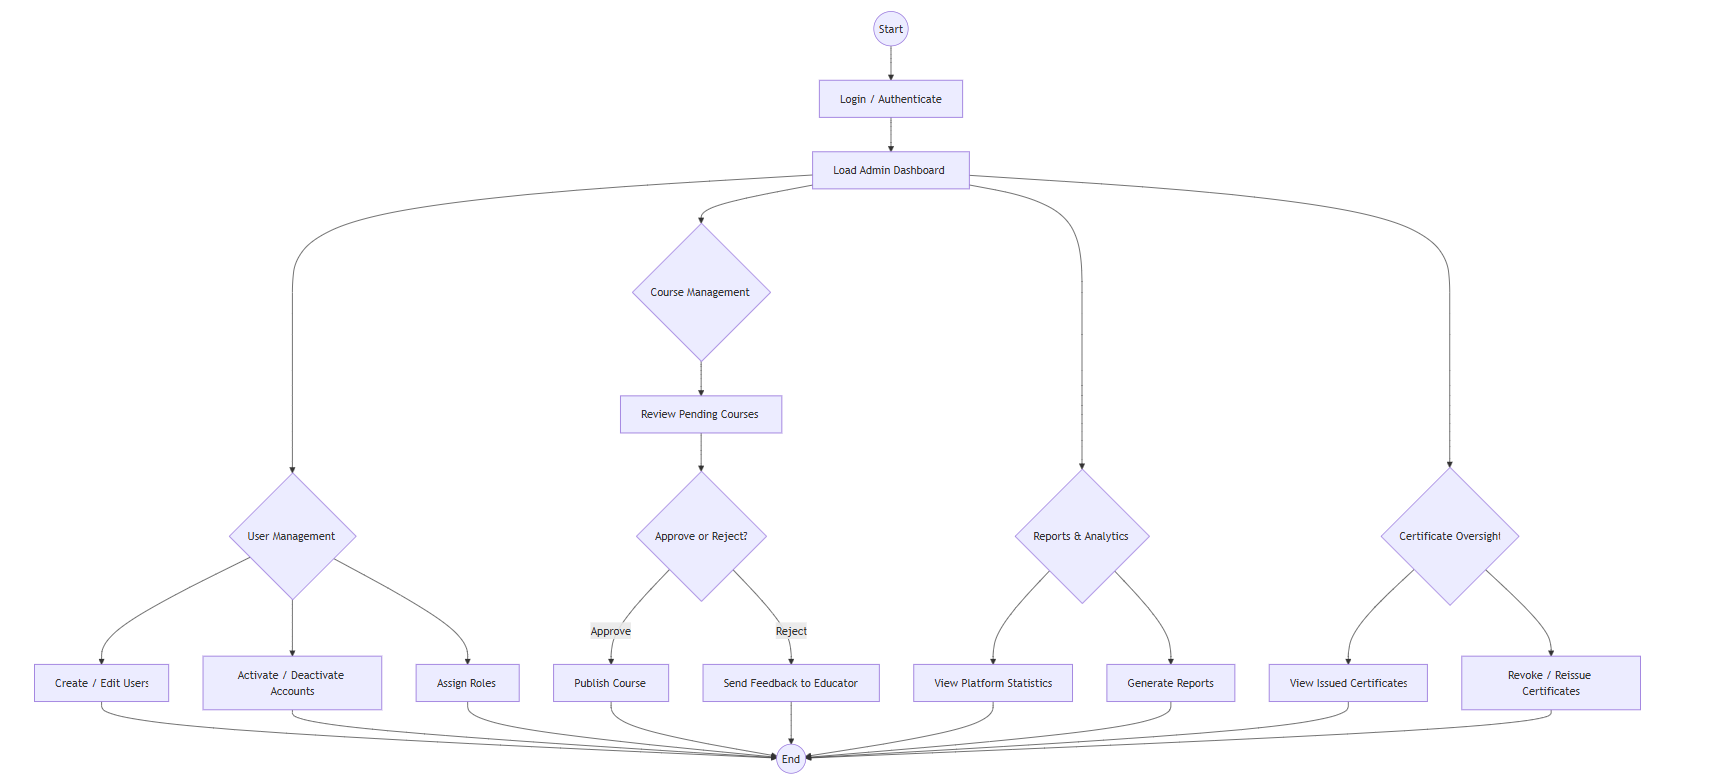
\includegraphics[width=0.75\textwidth,height=0.88\textheight,keepaspectratio]{Diagram/Figure 4.3 Administrator Activity Diagram.png}
\caption{Administrator Activity Diagram}
\label{fig:act_admin}
\end{figure}

The administrator workflow (Figure~\ref{fig:act_admin}) is primarily reactive. The administrator monitors two queues: courses awaiting review and applications from users wishing to become educators. When a course enters pending review, the administrator evaluates it, including against the course-level accessibility report. Approval sets its status to published, which fires the trigger that notifies the educator. Approving an educator application promotes the applicant, updating both the users table and the account's authentication metadata. Updating only one of the two previously left newly promoted educators unable to reach their own dashboard.

The remaining administrator activities are oversight rather than moderation: reviewing platform analytics, generating reports, managing user status, and handling enquiries submitted through the contact form.

\subsubsection{Interaction Design (Sequence Diagrams)}

Sequence diagrams detail how objects interact over time to execute specific use cases, mapping the calls between the client, the Next.js request interceptor, and the Supabase backend. One convention runs through all four: an operation drawn as reaching the database directly is one the client issues under its own session and Row-Level Security, while an operation drawn as passing through a server route is one that requires privileges the learner does not have. Which of the two a step uses is a security decision, not an implementation detail, so the diagrams distinguish them.

\paragraph{Sequence: Course Enrollment}

\begin{figure}[H]
\centering
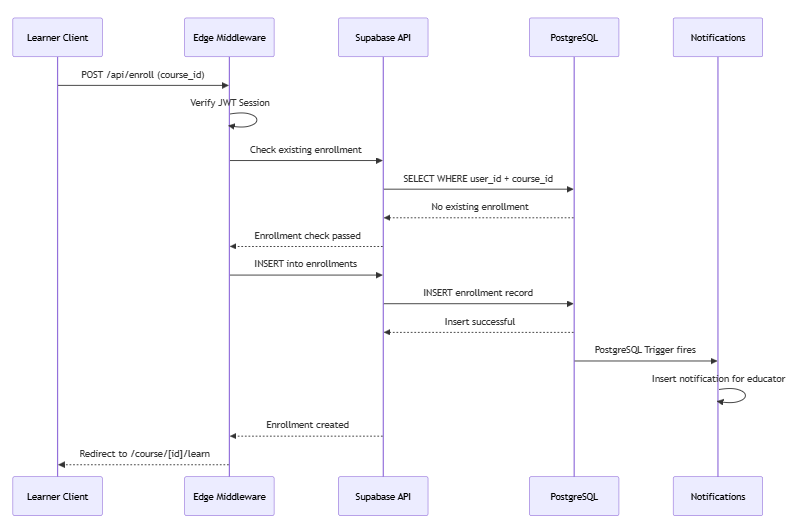
\includegraphics[width=0.75\textwidth,height=0.88\textheight,keepaspectratio]{Diagram/Figure 4.4 Course Enrollment Sequence Diagram.png}
\caption{Course Enrollment Sequence Diagram}
\label{fig:seq_enrollment}
\end{figure}

Figure~\ref{fig:seq_enrollment} illustrates the enrolment transaction. It is a good illustration of how little application code sits between the learner and the database in this architecture, and how much of the correctness is carried by the schema instead.

\begin{enumerate}
    \item The learner activates Enrol on a course page. The client calls Supabase directly under the anonymous key, since there is no bespoke enrolment endpoint, so the request carries the learner's own session and is evaluated under Row-Level Security.
    \item The database's insert policy on the enrolments table admits the new record only if the learner id on it matches the caller's own identity, so a learner cannot enrol anybody else. No application check is required for this, and none can be bypassed.
    \item A uniqueness constraint on the learner and course together prevents a duplicate enrolment. A repeat enrolment reactivates the existing record instead, preserving the learner's earlier progress.
    \item A database trigger fires and creates a notification addressed to the course's educator.
    \item The client navigates to the course page, which now renders the lesson roadmap rather than the enrolment call to action.
\end{enumerate}

\paragraph{Sequence: Lesson Learning \& Telemetry}

\begin{figure}[H]
\centering
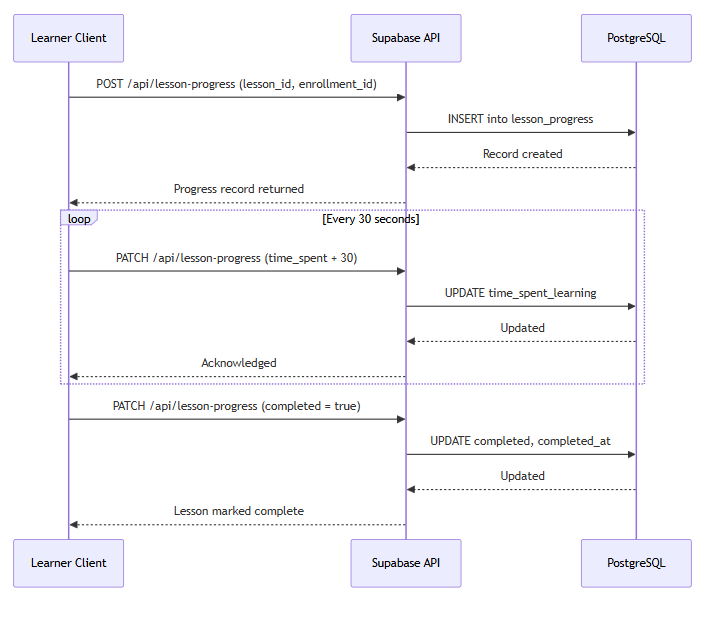
\includegraphics[width=0.75\textwidth,height=0.88\textheight,keepaspectratio]{Diagram/Figure 4.5 Lesson Learning Sequence Diagram.png}
\caption{Lesson Learning Sequence Diagram}
\label{fig:seq_lesson}
\end{figure}

Figure~\ref{fig:seq_lesson} maps lesson telemetry. Opening a lesson creates or updates the learner's progress record for it, marking the lesson viewed, incrementing the view count and stamping the time it was first opened. While the lesson remains open, elapsed time is accumulated periodically into that record rather than being written only when the page unloads, so that a browser closed abruptly still leaves an accurate record up to the last interval rather than losing the whole session.

Completion is recorded separately from viewing, and the two are constrained to remain consistent. A database check rejects any progress record marked complete but not viewed. This distinction matters to the recommendation engine, which keys what a learner should do next on completion rather than on viewing. Keying it on viewing instead would skip every lesson the learner had merely glanced at.

\paragraph{Sequence: Quiz Attempt \& Adaptive Recommendation}

\begin{figure}[H]
\centering
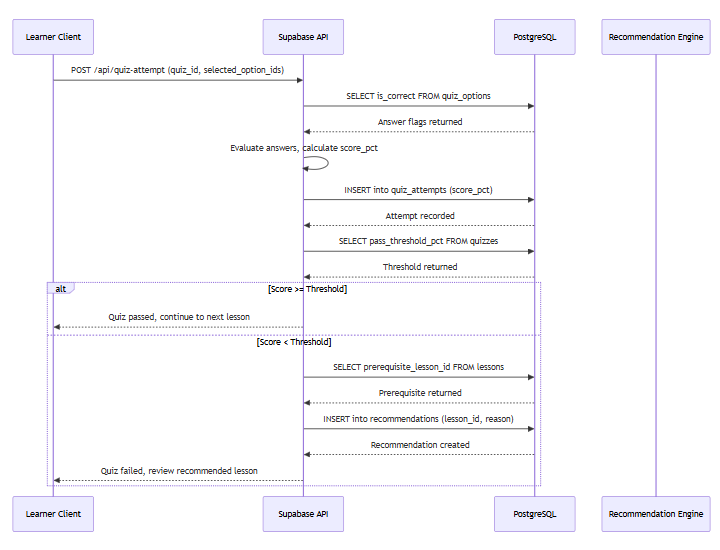
\includegraphics[width=0.75\textwidth,height=0.88\textheight,keepaspectratio]{Diagram/Figure 4.6 Quiz Attempt Sequence Diagram.png}
\caption{Quiz Attempt Sequence Diagram}
\label{fig:seq_quiz}
\end{figure}

Figure~\ref{fig:seq_quiz} details the most security-sensitive interaction in the system, and the one where the design most deliberately refuses to trust the client.

\begin{enumerate}
    \item While answering, the client reads options from a restricted database view rather than the underlying options table. That view withholds which option is correct for any quiz the learner has not yet submitted, so the answer key is not present in the client at all. It is not merely hidden. It is absent.
    \item On submission the client calls a database grading function with the quiz identifier and the selected options. It does not compute a score and does not write an attempt record itself. A guard trigger would reject the write if it tried.
    \item The function verifies authentication, verifies an active enrolment in the owning course, and refuses the attempt if the quiz's attempt limit is exhausted.
    \item It grades each answer against the stored correctness flag, writes the attempt and its answers to the database, and computes the pass decision against the quiz's pass threshold. It returns the score, the pass decision and the threshold used, so the interface can explain the result rather than merely report it.
    \item A database trigger raises a notification for the educator.
    \item The answer key becomes readable to that learner for that quiz only now, which is what allows the review screen to show which answers were wrong.
    \item Separately, the recommendation engine records a revision-tier recommendation for the lesson, carrying the score that triggered it as its stated reason.
\end{enumerate}

\paragraph{Sequence: Course Creation \& Media Upload}

\begin{figure}[H]
\centering
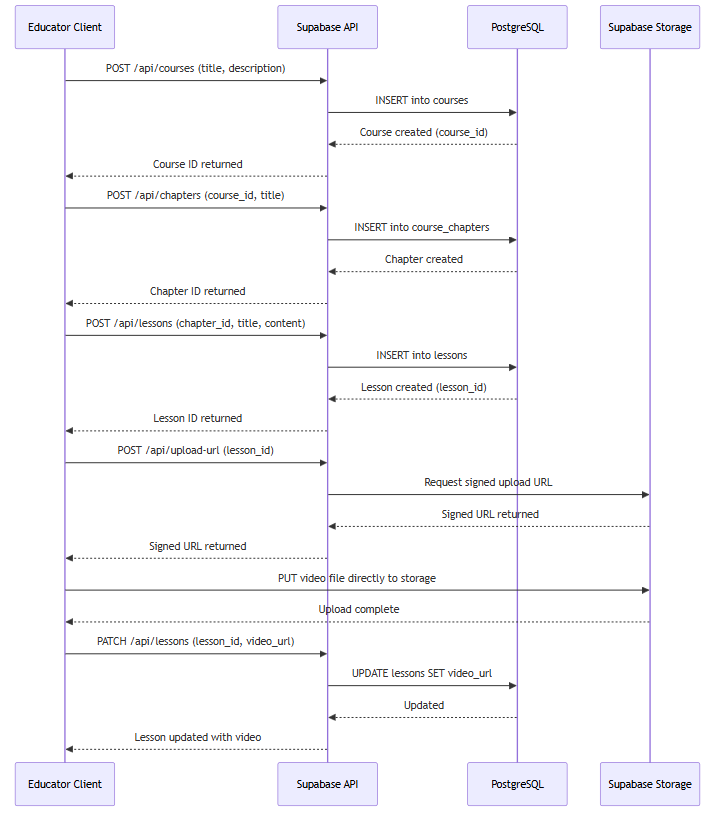
\includegraphics[width=0.75\textwidth,height=0.88\textheight,keepaspectratio]{Diagram/Figure 4.7 Course Creation Sequence Diagram.png}
\caption{Course Creation Sequence Diagram}
\label{fig:seq_course_creation}
\end{figure}

Figure~\ref{fig:seq_course_creation} shows the authoring pipeline. Lesson text is composed in the rich-text editor, sanitised, and written to the lesson's content field, with a snapshot appended to the version history so that an edit is recoverable. Images and documents are uploaded from the client straight into cloud storage, bypassing the application server so that a large file never has to be buffered by it, and the returned public URL is recorded against the course's media assets.

Instructional video is handled differently, and the distinction matters for the storage and cost model. Video is \emph{embedded from an external host} by URL rather than uploaded, so the lesson holds only a reference to a resource the platform does not store or serve. Throughout this pipeline the auditor re-runs on every change, so the accessibility consequence of an edit, such as adding a video without a transcript, is visible at the moment it is made rather than at publication.

\subsubsection{User Interface Design}
\label{sec:ui-design}
\setcounter{uidsub}{0}

The interface architecture of ACESS is organised into three role-specific shells, each with its own navigation structure, input mechanisms and output presentation. Every figure in this section is a screenshot of the running system taken against the reproducible demonstration database described in Section~\ref{sec:phys-db}, not a mockup.

\uidesignsub{Navigation Design}

Navigation follows a role-based shell pattern. The route prefix determines the shell, and a server-side check refuses a shell the signed-in role is not entitled to before the page renders.

\begin{itemize}
    \item \textbf{Public navigation.} Unauthenticated visitors reach the landing page, the course catalogue preview, login, signup, password recovery, the contact form, the educator-application form, and the published accessibility statement. Certificate verification (\tcode{/verify/[code]}) is also public, so that a third party can check a certificate without an account.
    \item \textbf{Learner shell.} A persistent sidebar carries Dashboard, My Courses, Progress, Achievements \& Certificates, and Accessibility. A top bar holds the notification bell with an unread count and the profile menu. Two things about this sidebar are design decisions rather than defaults. First, every item is a real hyperlink rather than a click handler, so that a screen reader announces navigation as navigation and the browser's own affordances (middle-click, open in a new tab, copy link) work. Second, the sidebar's contents are \emph{preset-dependent}: the Dyslexia preset widens it and enlarges its type, and the distraction-free presets remove it entirely inside a lesson.
    \item \textbf{Educator shell.} A sidebar carries Dashboard, Courses (All Courses, My Courses, Add Course), Educator Ranking, Analytics, Students Progress and Certificates. Inside a course, a workspace tab bar provides Overview, Lessons, Assets, Students, Certificates, Achievements and Settings.
    \item \textbf{Administrator shell.} A sidebar carries Dashboard, User Management, Course Management, Educators (educator applications), Feedback (contact messages), Certificates, Analytics and Reports.
\end{itemize}

\begin{figure}[H]
\centering
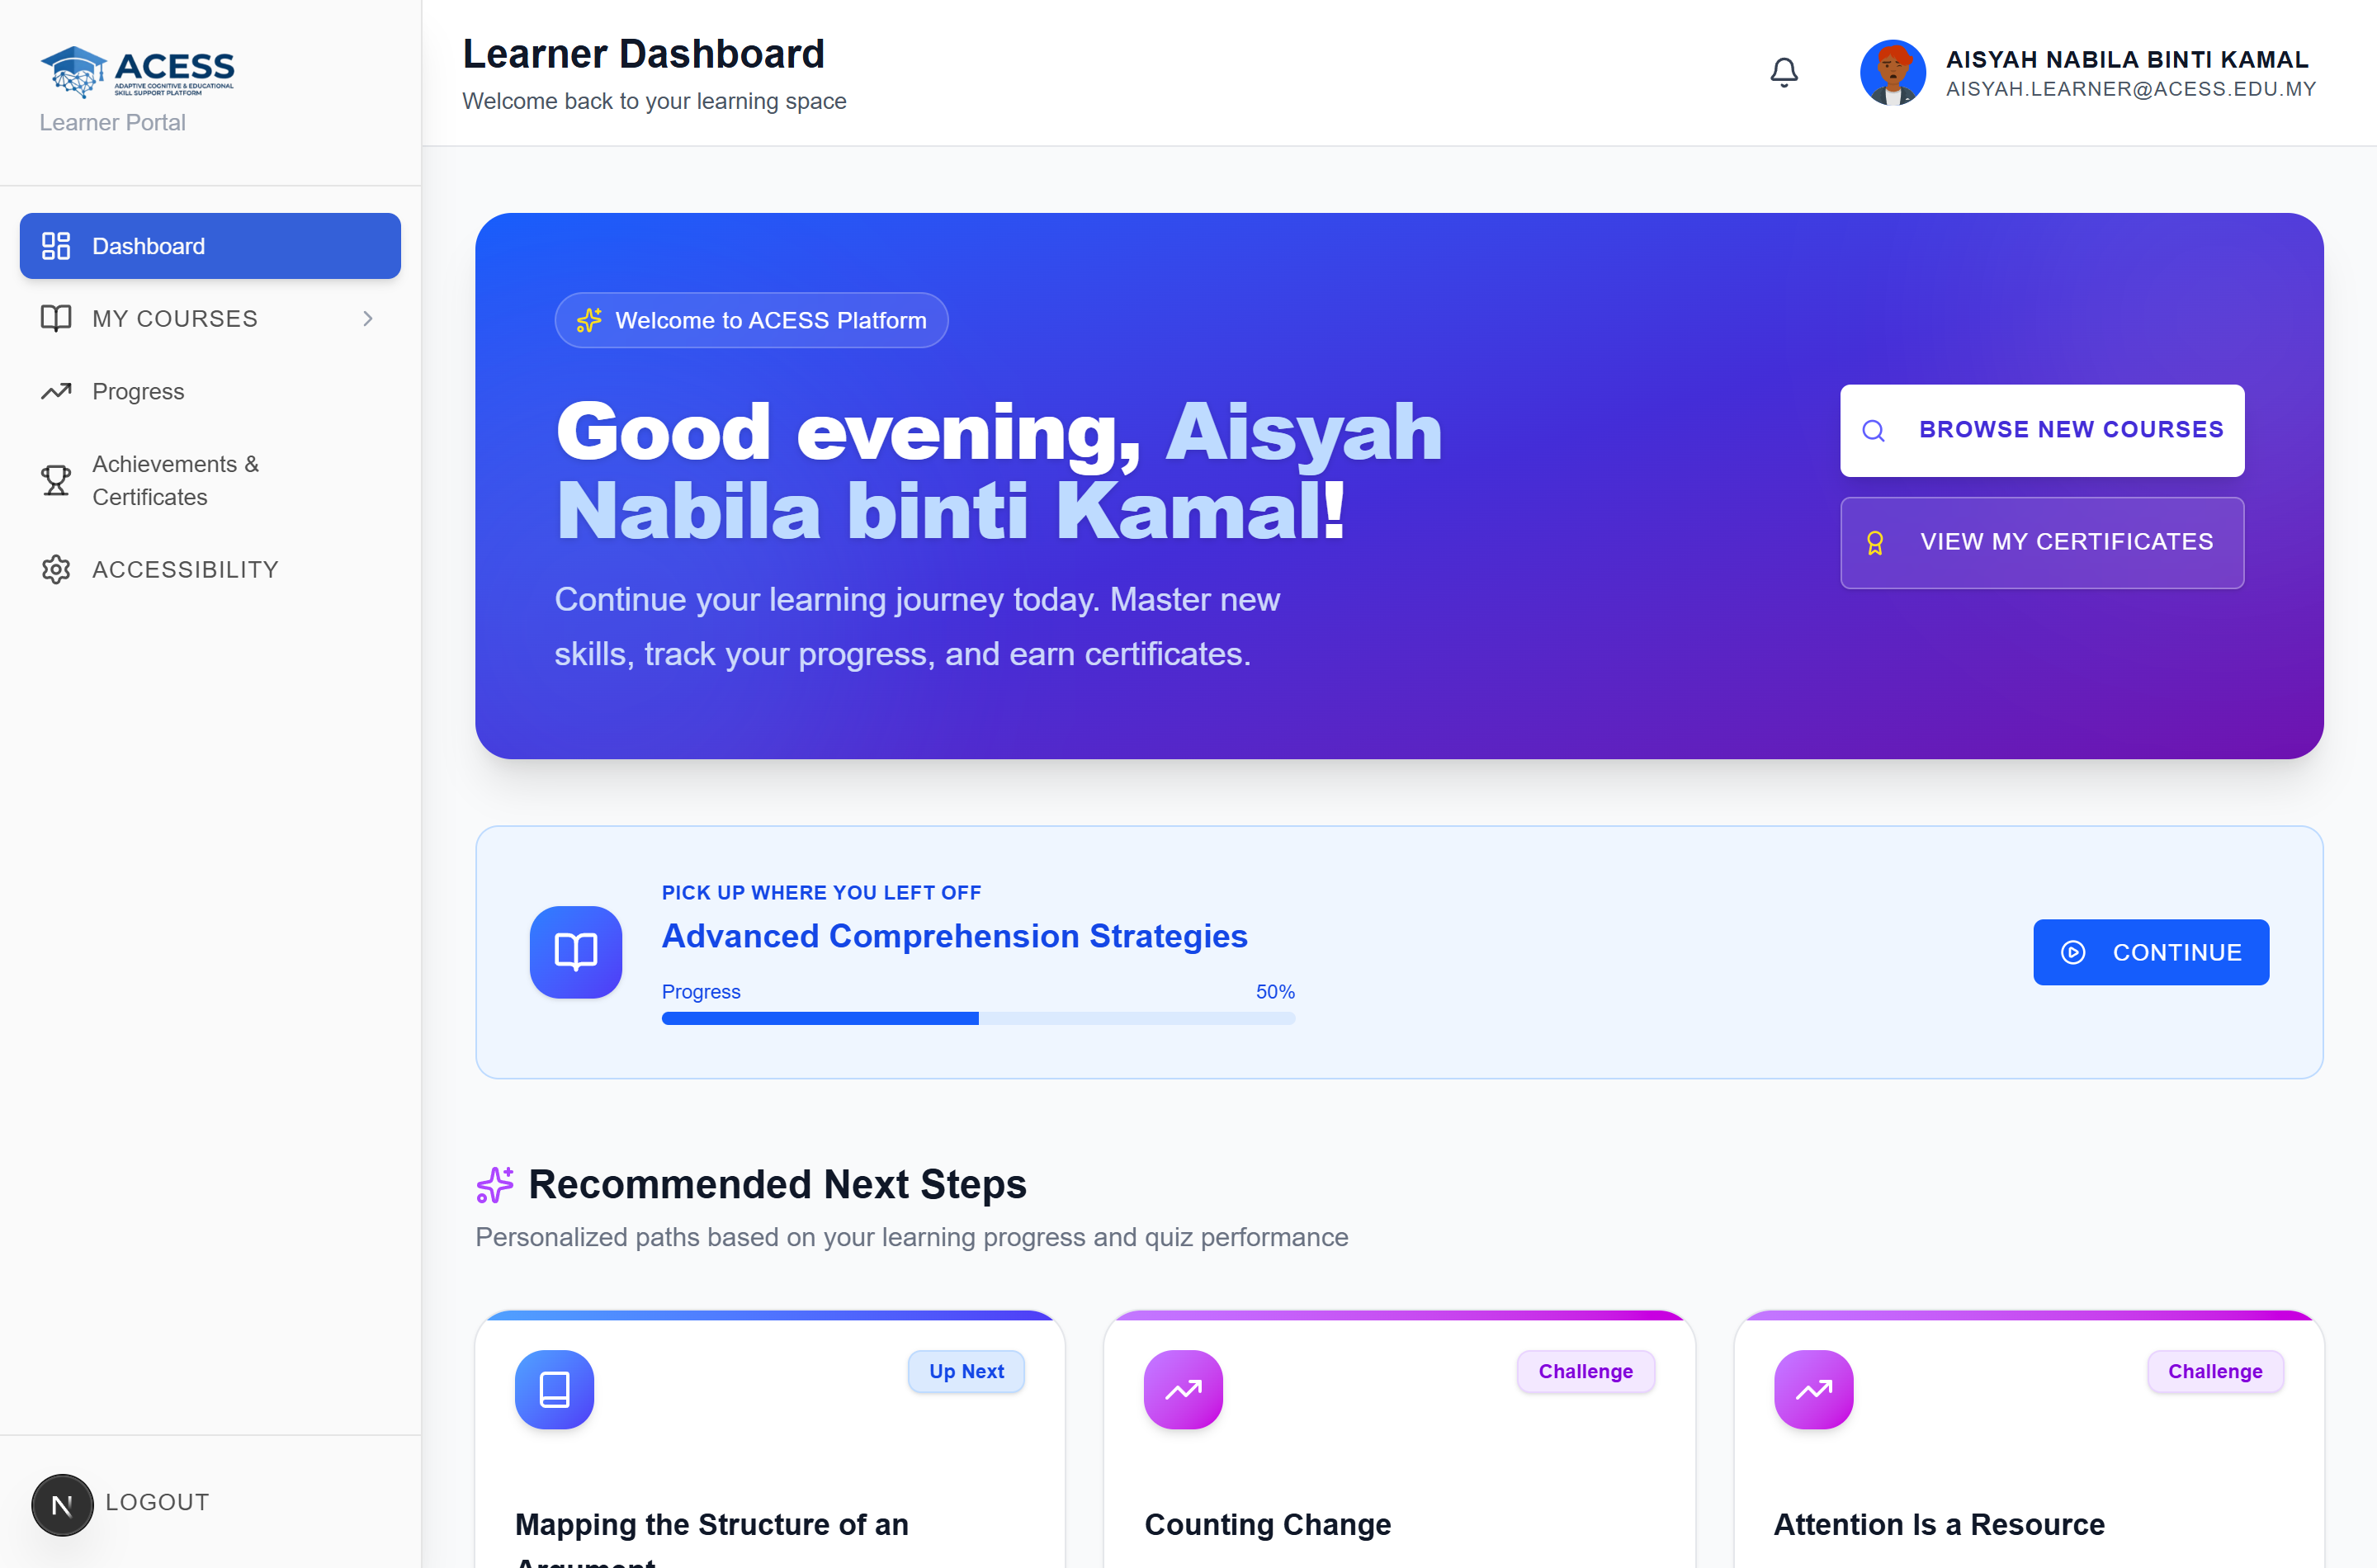
\includegraphics[width=0.92\textwidth]{Screenshots/dashboard-none.png}
\caption{Learner Dashboard (Default State)}
\label{fig:ui_learner_dashboard}
\end{figure}

Figure~\ref{fig:ui_learner_dashboard} shows the learner dashboard as a learner with no accessibility preset applied encounters it, with its persistent sidebar, continue-learning card and recommendation region visible together. The corresponding educator workspace is shown in Figure~\ref{fig:ui_edu_workspace}, where the workspace tab bar and the ordered lesson curriculum are visible together with the per-lesson authoring controls.

\begin{figure}[H]
\centering
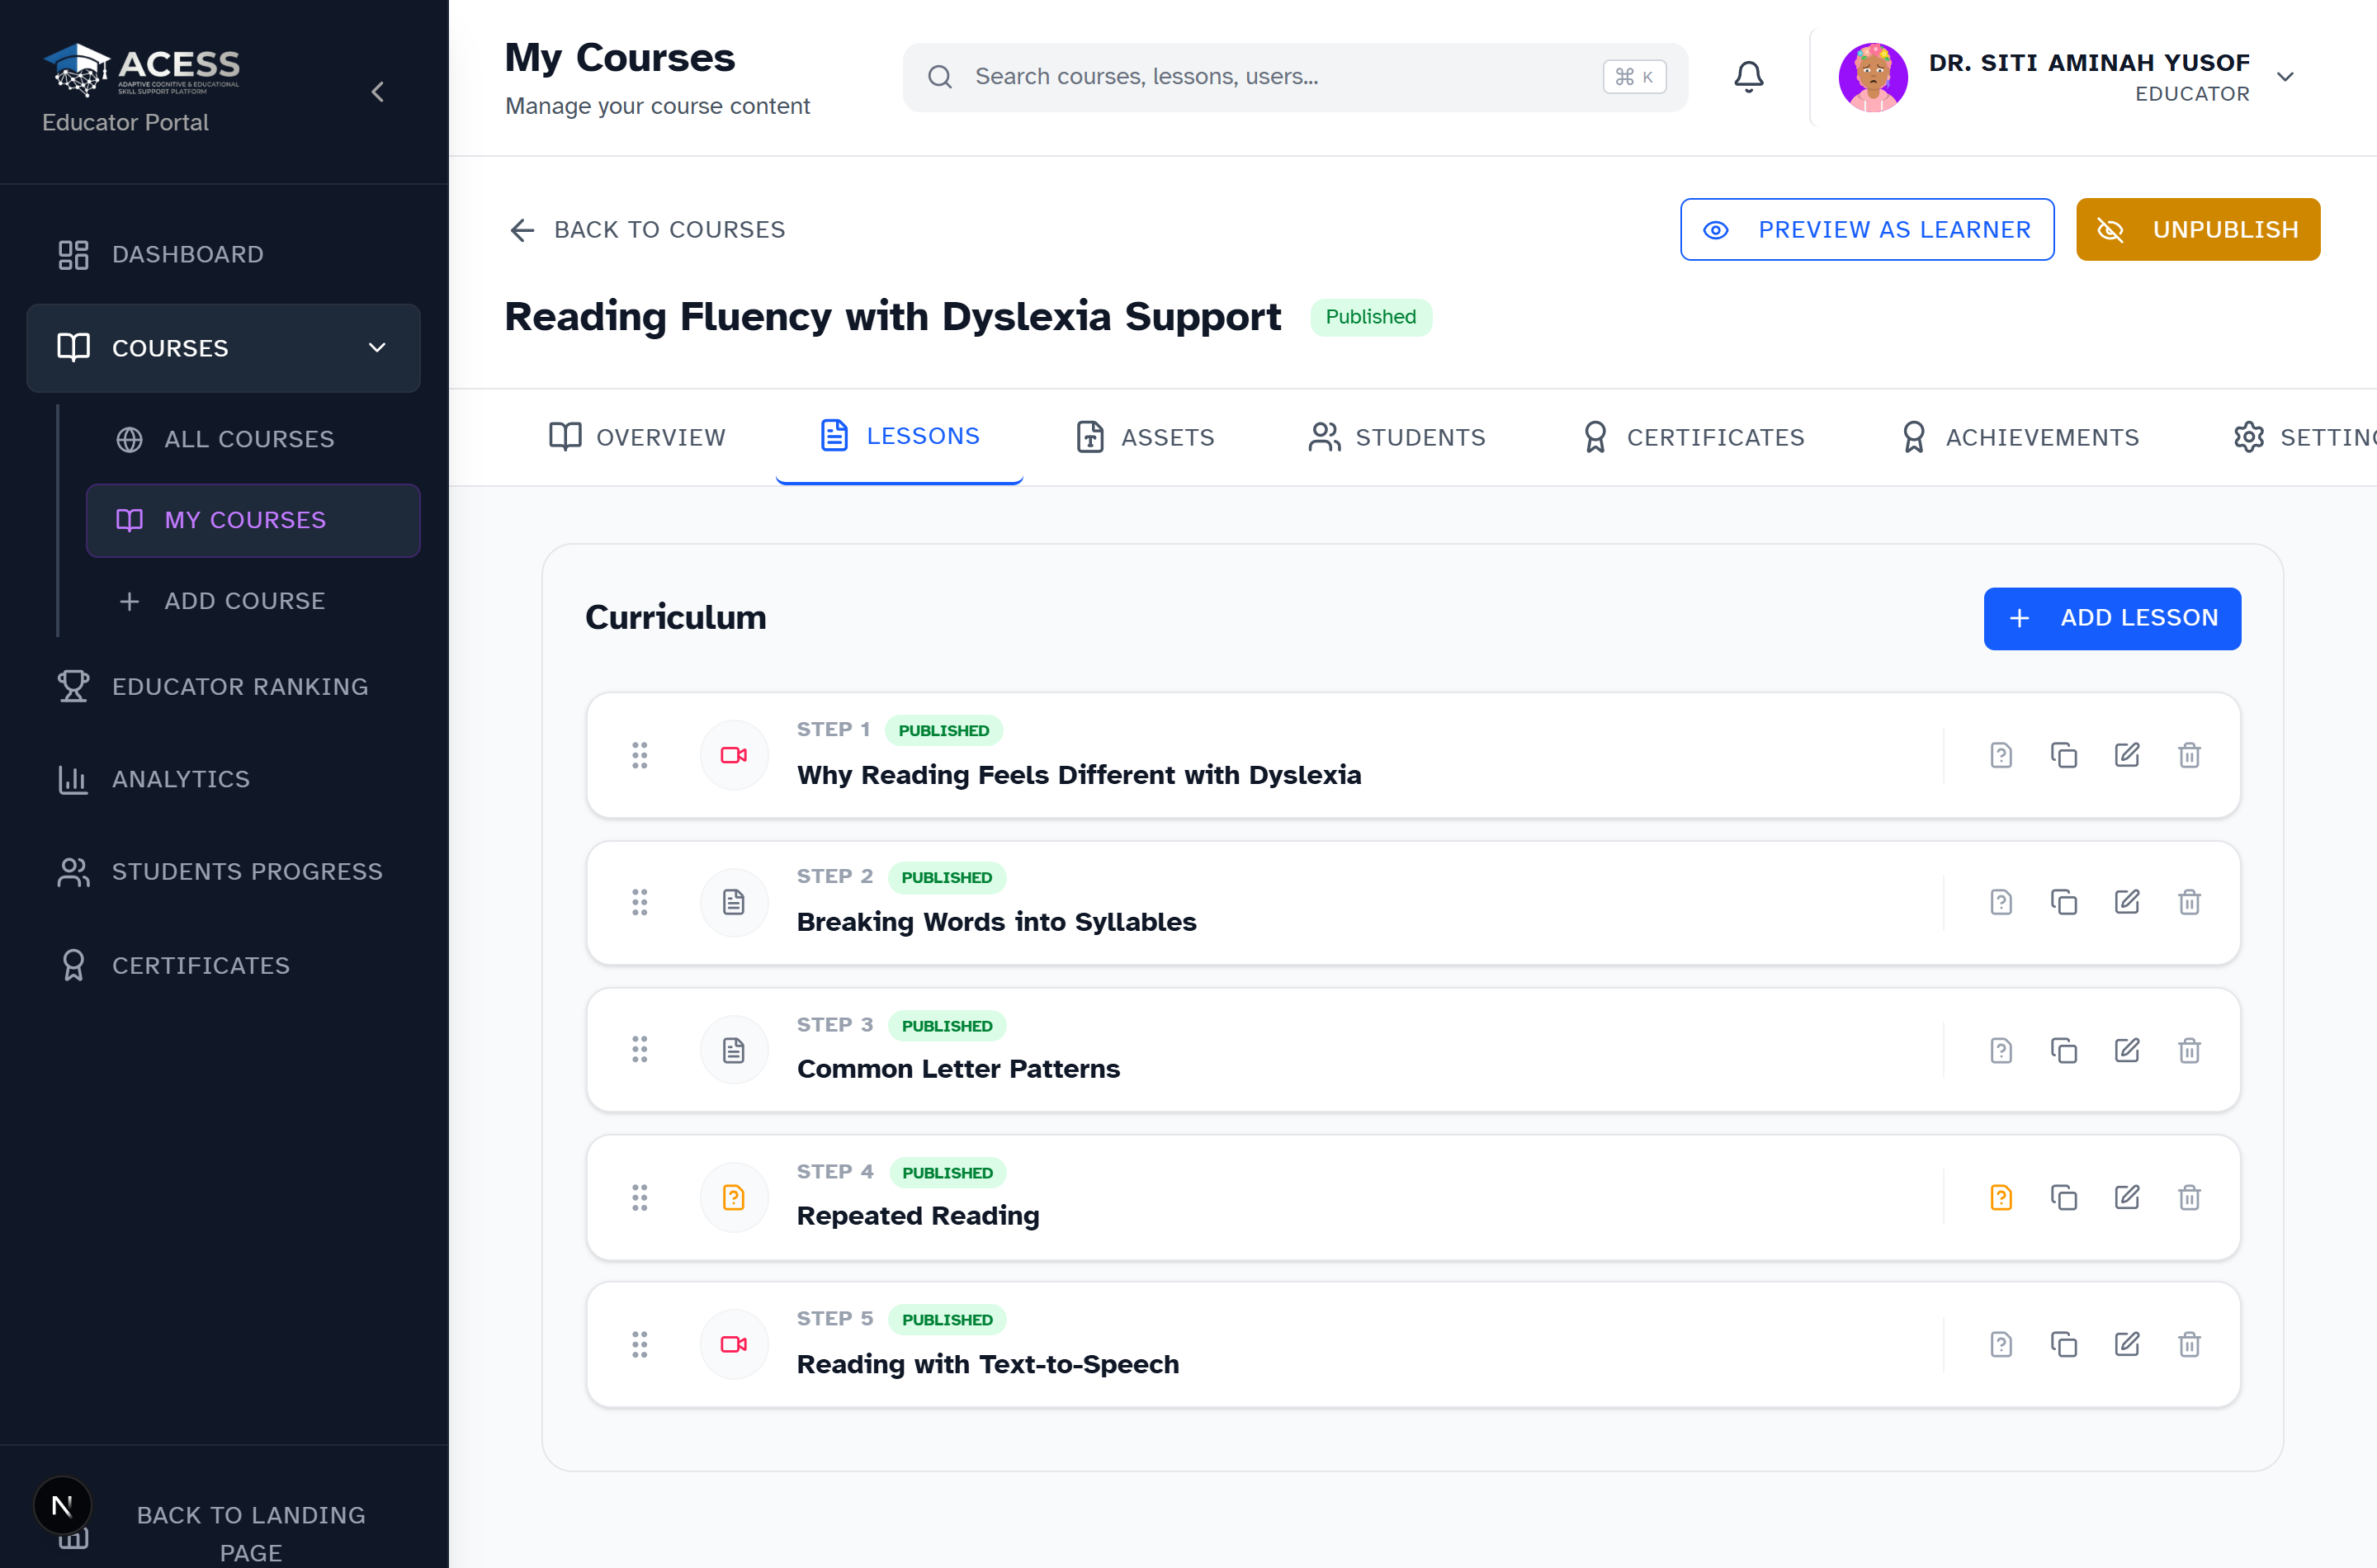
\includegraphics[width=0.92\textwidth]{Screenshots/educator-course-workspace.png}
\caption{Educator Course Workspace (Lessons Tab)}
\label{fig:ui_edu_workspace}
\end{figure}

\uidesignsub{Input Design}

Input surfaces are grouped below by the role that uses them, matching the structure of Navigation Design above.

\begin{itemize}
    \item \textbf{Public input.} An unauthenticated visitor supplies an email and password at sign-up, and a category, subject and message on the contact form. A visitor's requested role is never accepted from the sign-up request itself: self-registration is always pinned to the learner role by a database trigger.
    \item \textbf{Learner input.} A learner selects a course to enrol in, adjusts accessibility settings such as font size and line spacing from the accessibility panel (Figure~\ref{fig:ui_a11y_modal}), answers quiz questions (Figure~\ref{fig:ui_quiz}), and uploads a profile avatar.
    \item \textbf{Educator input.} An educator supplies course metadata such as title, slug, difficulty and status, writes lesson content in the rich-text editor, sets the sequence order and layout of each lesson, and builds quiz questions and their options.
    \item \textbf{Administrator input.} An administrator sets a target user's role, decides whether a submitted course is approved or rejected, and selects the date range for a platform report.
\end{itemize}

Table~\ref{tab:input_validation} then states the exact validation rule applied to each significant field above and the layer at which it is enforced. The distinction matters: a rule enforced only in the browser is a convenience, whereas a rule enforced by a database constraint or an RLS policy cannot be bypassed by a crafted request.

{
\renewcommand{\arraystretch}{1.2}
\footnotesize
\begin{longtable}{|>{\raggedright\arraybackslash\tabbreak}p{2.43cm}|>{\raggedright\arraybackslash\tabbreak}p{2.89cm}|>{\raggedright\arraybackslash\tabbreak}p{4.29cm}|>{\raggedright\arraybackslash\tabbreak}p{3.17cm}|}
\caption{Input Validation Rules}
\label{tab:input_validation}\\
\hline
\textbf{Screen} & \textbf{Field} & \textbf{Validation rule} & \textbf{Enforced at} \\
\hline \hline
\endfirsthead
\multicolumn{4}{l}{\footnotesize\itshape Table~\ref{tab:input_validation} continued from the previous page}\\
\hline
\textbf{Screen} & \textbf{Field} & \textbf{Validation rule} & \textbf{Enforced at} \\
\hline \hline
\endhead
\hline
\multicolumn{4}{r}{\footnotesize\itshape continued on the next page}\\
\endfoot
\endlastfoot
Sign up & Email & Well-formed address, must be unique & Client, then Supabase Auth \\ \hline
Sign up & Password & Minimum length and complexity & Client, then Supabase Auth \\ \hline
Sign up & Role & Always \tcode{learner}, not accepted from the request & Database trigger \\ \hline
Course form & Title & Required, non-blank & Client + \texttt{NOT NULL} \\ \hline
Course form & Slug & Unique across courses & \texttt{UNIQUE} constraint \\ \hline
Course form & Difficulty & One of beginner / intermediate / advanced & \texttt{CHECK} constraint \\ \hline
Course form & Status & One of draft / pending\_review / published / archived & \texttt{CHECK} constraint \\ \hline
Lesson editor & Rich text & Sanitised before render, disallowed markup stripped & Client sanitiser \\ \hline
Lesson editor & Sequence order & Integer greater than zero & \texttt{CHECK} constraint \\ \hline
Lesson editor & Lesson layout & One of standard / focus / two\_column / wide / slideshow & \texttt{CHECK} constraint \\ \hline
Quiz builder & Pass threshold & Integer between 0 and 100 & \texttt{CHECK} constraint \\ \hline
Quiz builder & Options & At least two options, exactly one correct & Client \\ \hline
Quiz attempt & Selected options & Graded server-side, answer key never sent early & Database function + view \\ \hline
Accessibility panel & Font size & Slider bounded 12--24\,px & Client \\ \hline
Accessibility panel & Line spacing & Slider bounded 1.0--3.0 & Client \\ \hline
Enrolment & Course reference & Learner may only enrol themselves & RLS policy \\ \hline
Enrolment & Status & One of active / completed / dropped, completion not client-settable & \texttt{CHECK} + guard trigger \\ \hline
Contact form & Category & One of five permitted categories & \texttt{CHECK} constraint \\ \hline
Avatar upload & File path & Must sit inside the uploader's own folder & Storage policy \\ \hline
\end{longtable}
}

The single most important input surface in the system is the accessibility panel, shown in Figure~\ref{fig:ui_a11y_modal}. It presents four preset buttons above five tabbed groups (Reading, Focus, Sensory, Supports and Profile), and every control writes through to the learner's stored preferences and takes effect without a page reload.

\begin{figure}[H]
\centering
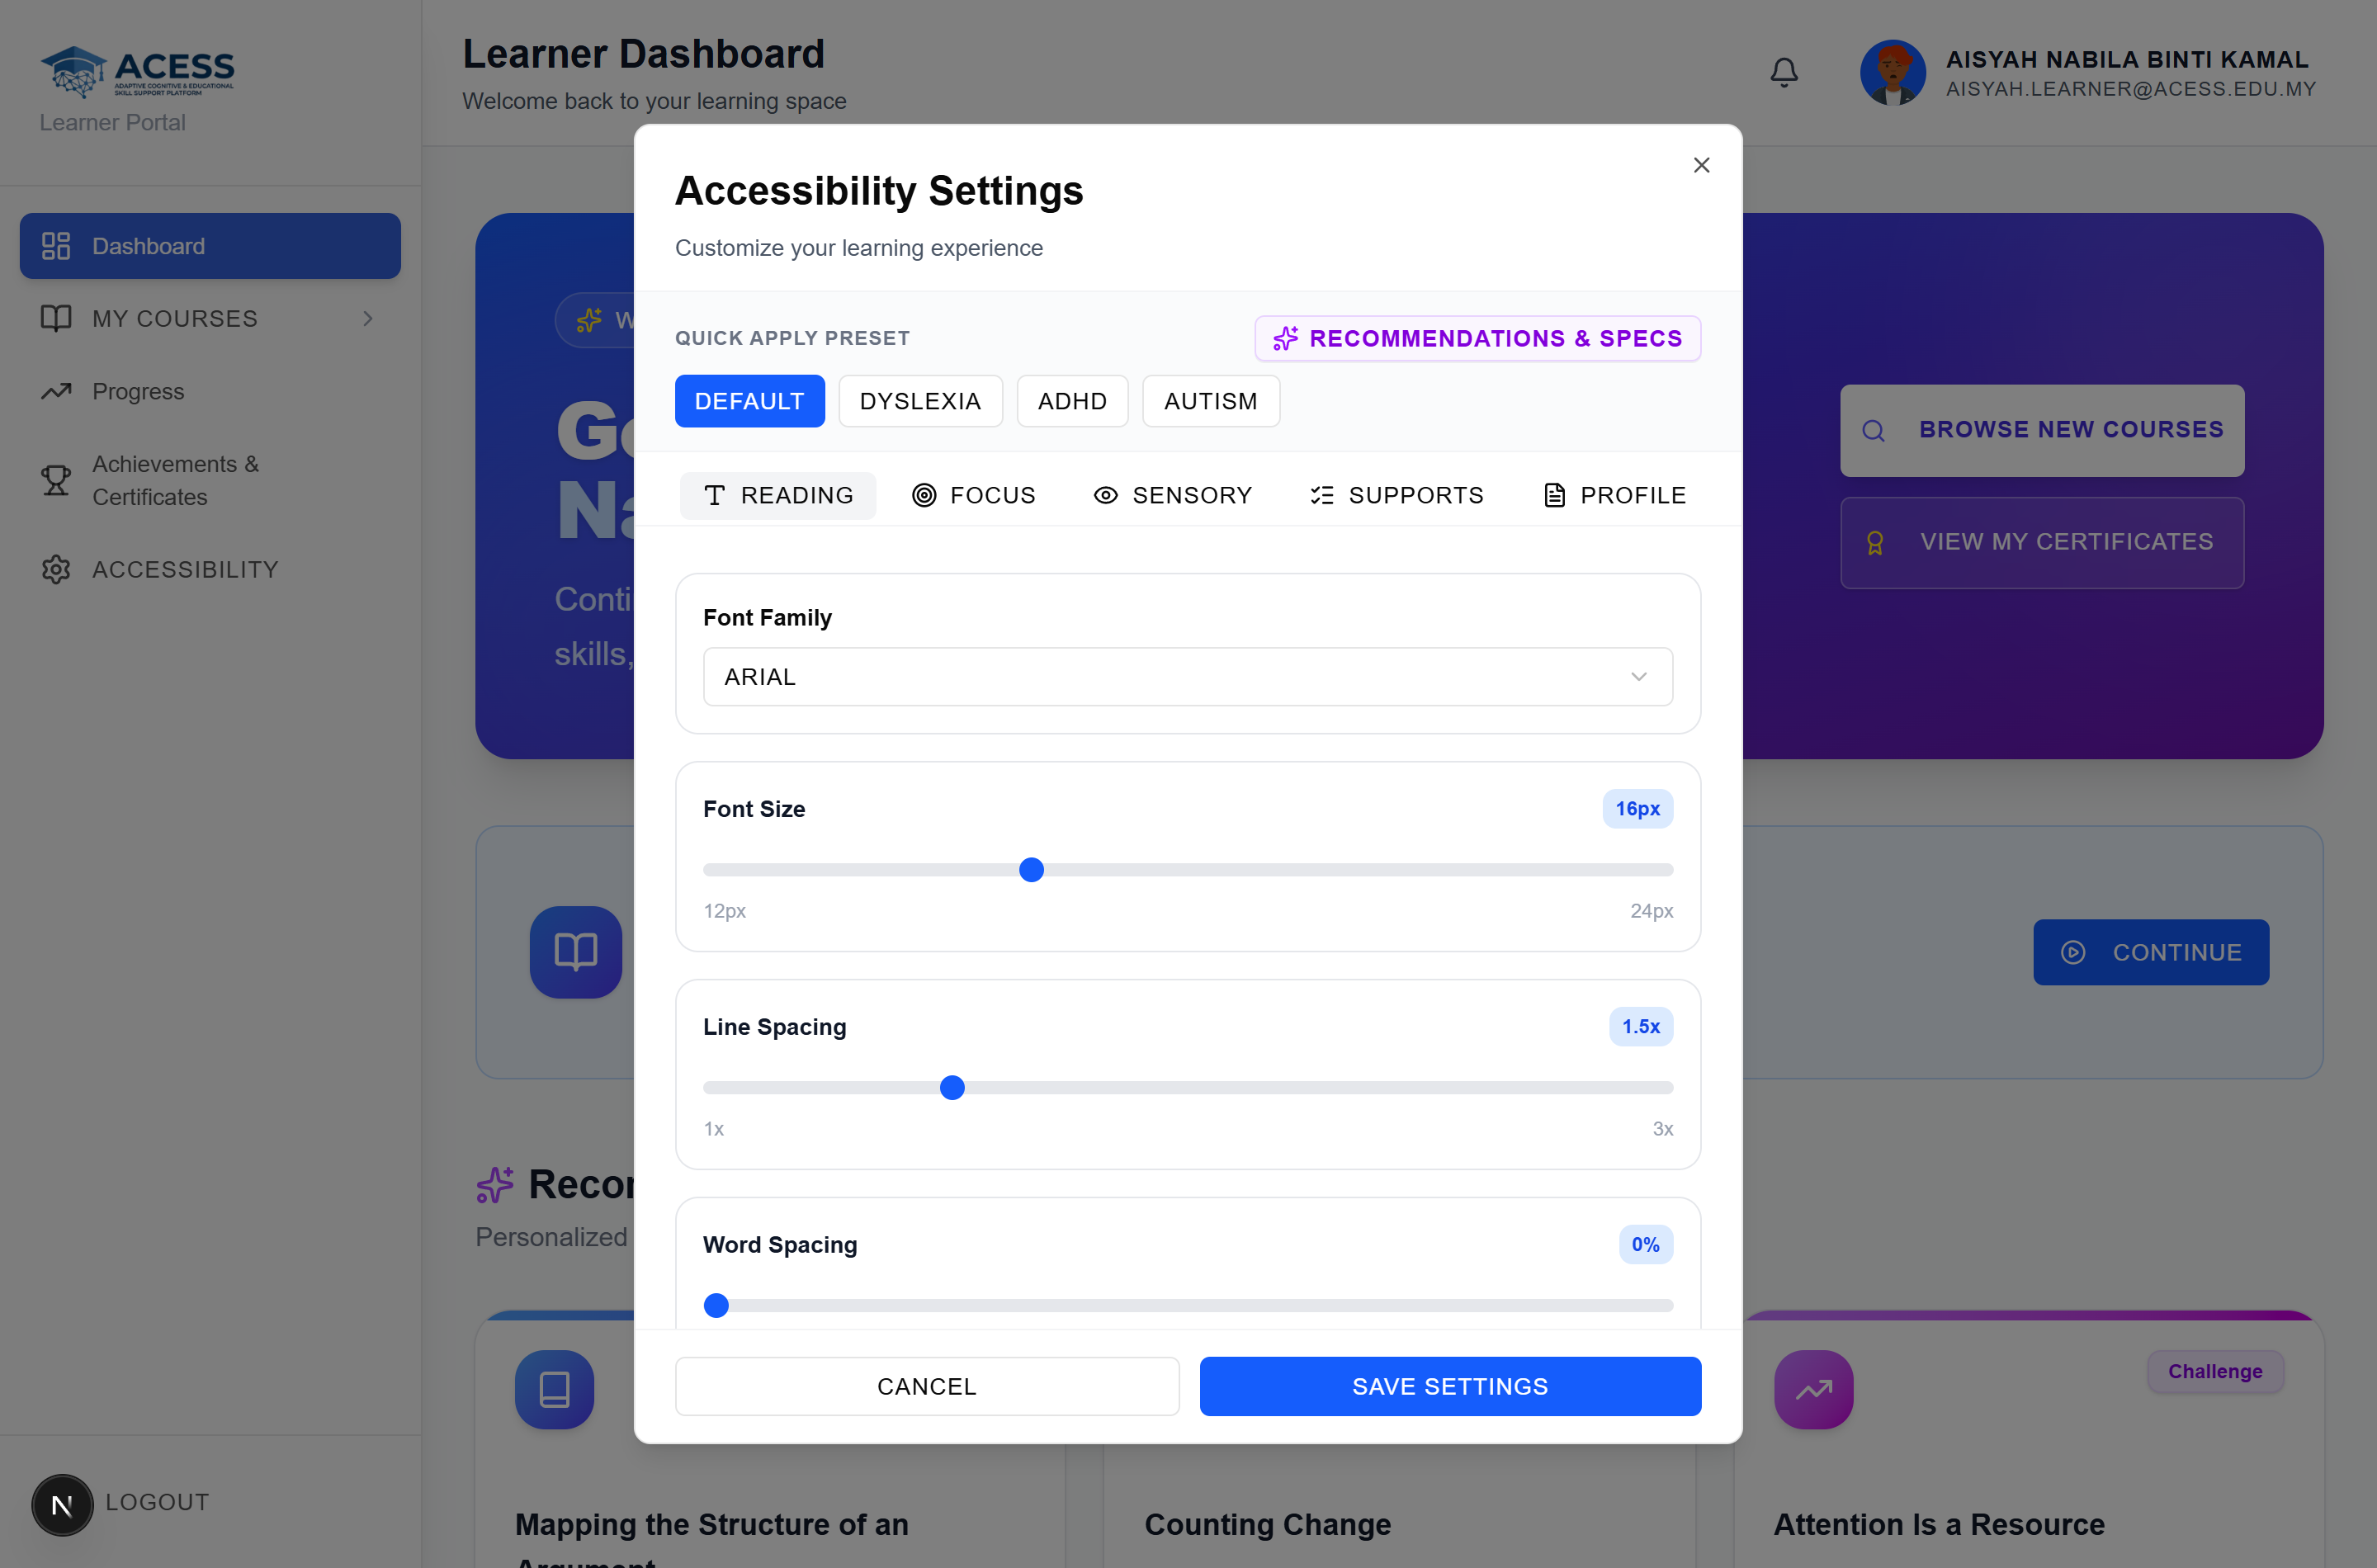
\includegraphics[width=0.92\textwidth]{Screenshots/a11y-settings-modal.png}
\caption{Accessibility Settings Panel (Reading Group)}
\label{fig:ui_a11y_modal}
\end{figure}

The second significant input surface is the quiz, shown in Figure~\ref{fig:ui_quiz}. Its design carries three deliberate accessibility decisions: questions are presented one per screen regardless of the lesson's own layout setting, an educator-configured time limit is displayed but never triggers an automatic submission, and the expectations for the attempt are stated before it begins rather than discovered during it.

\begin{figure}[H]
\centering
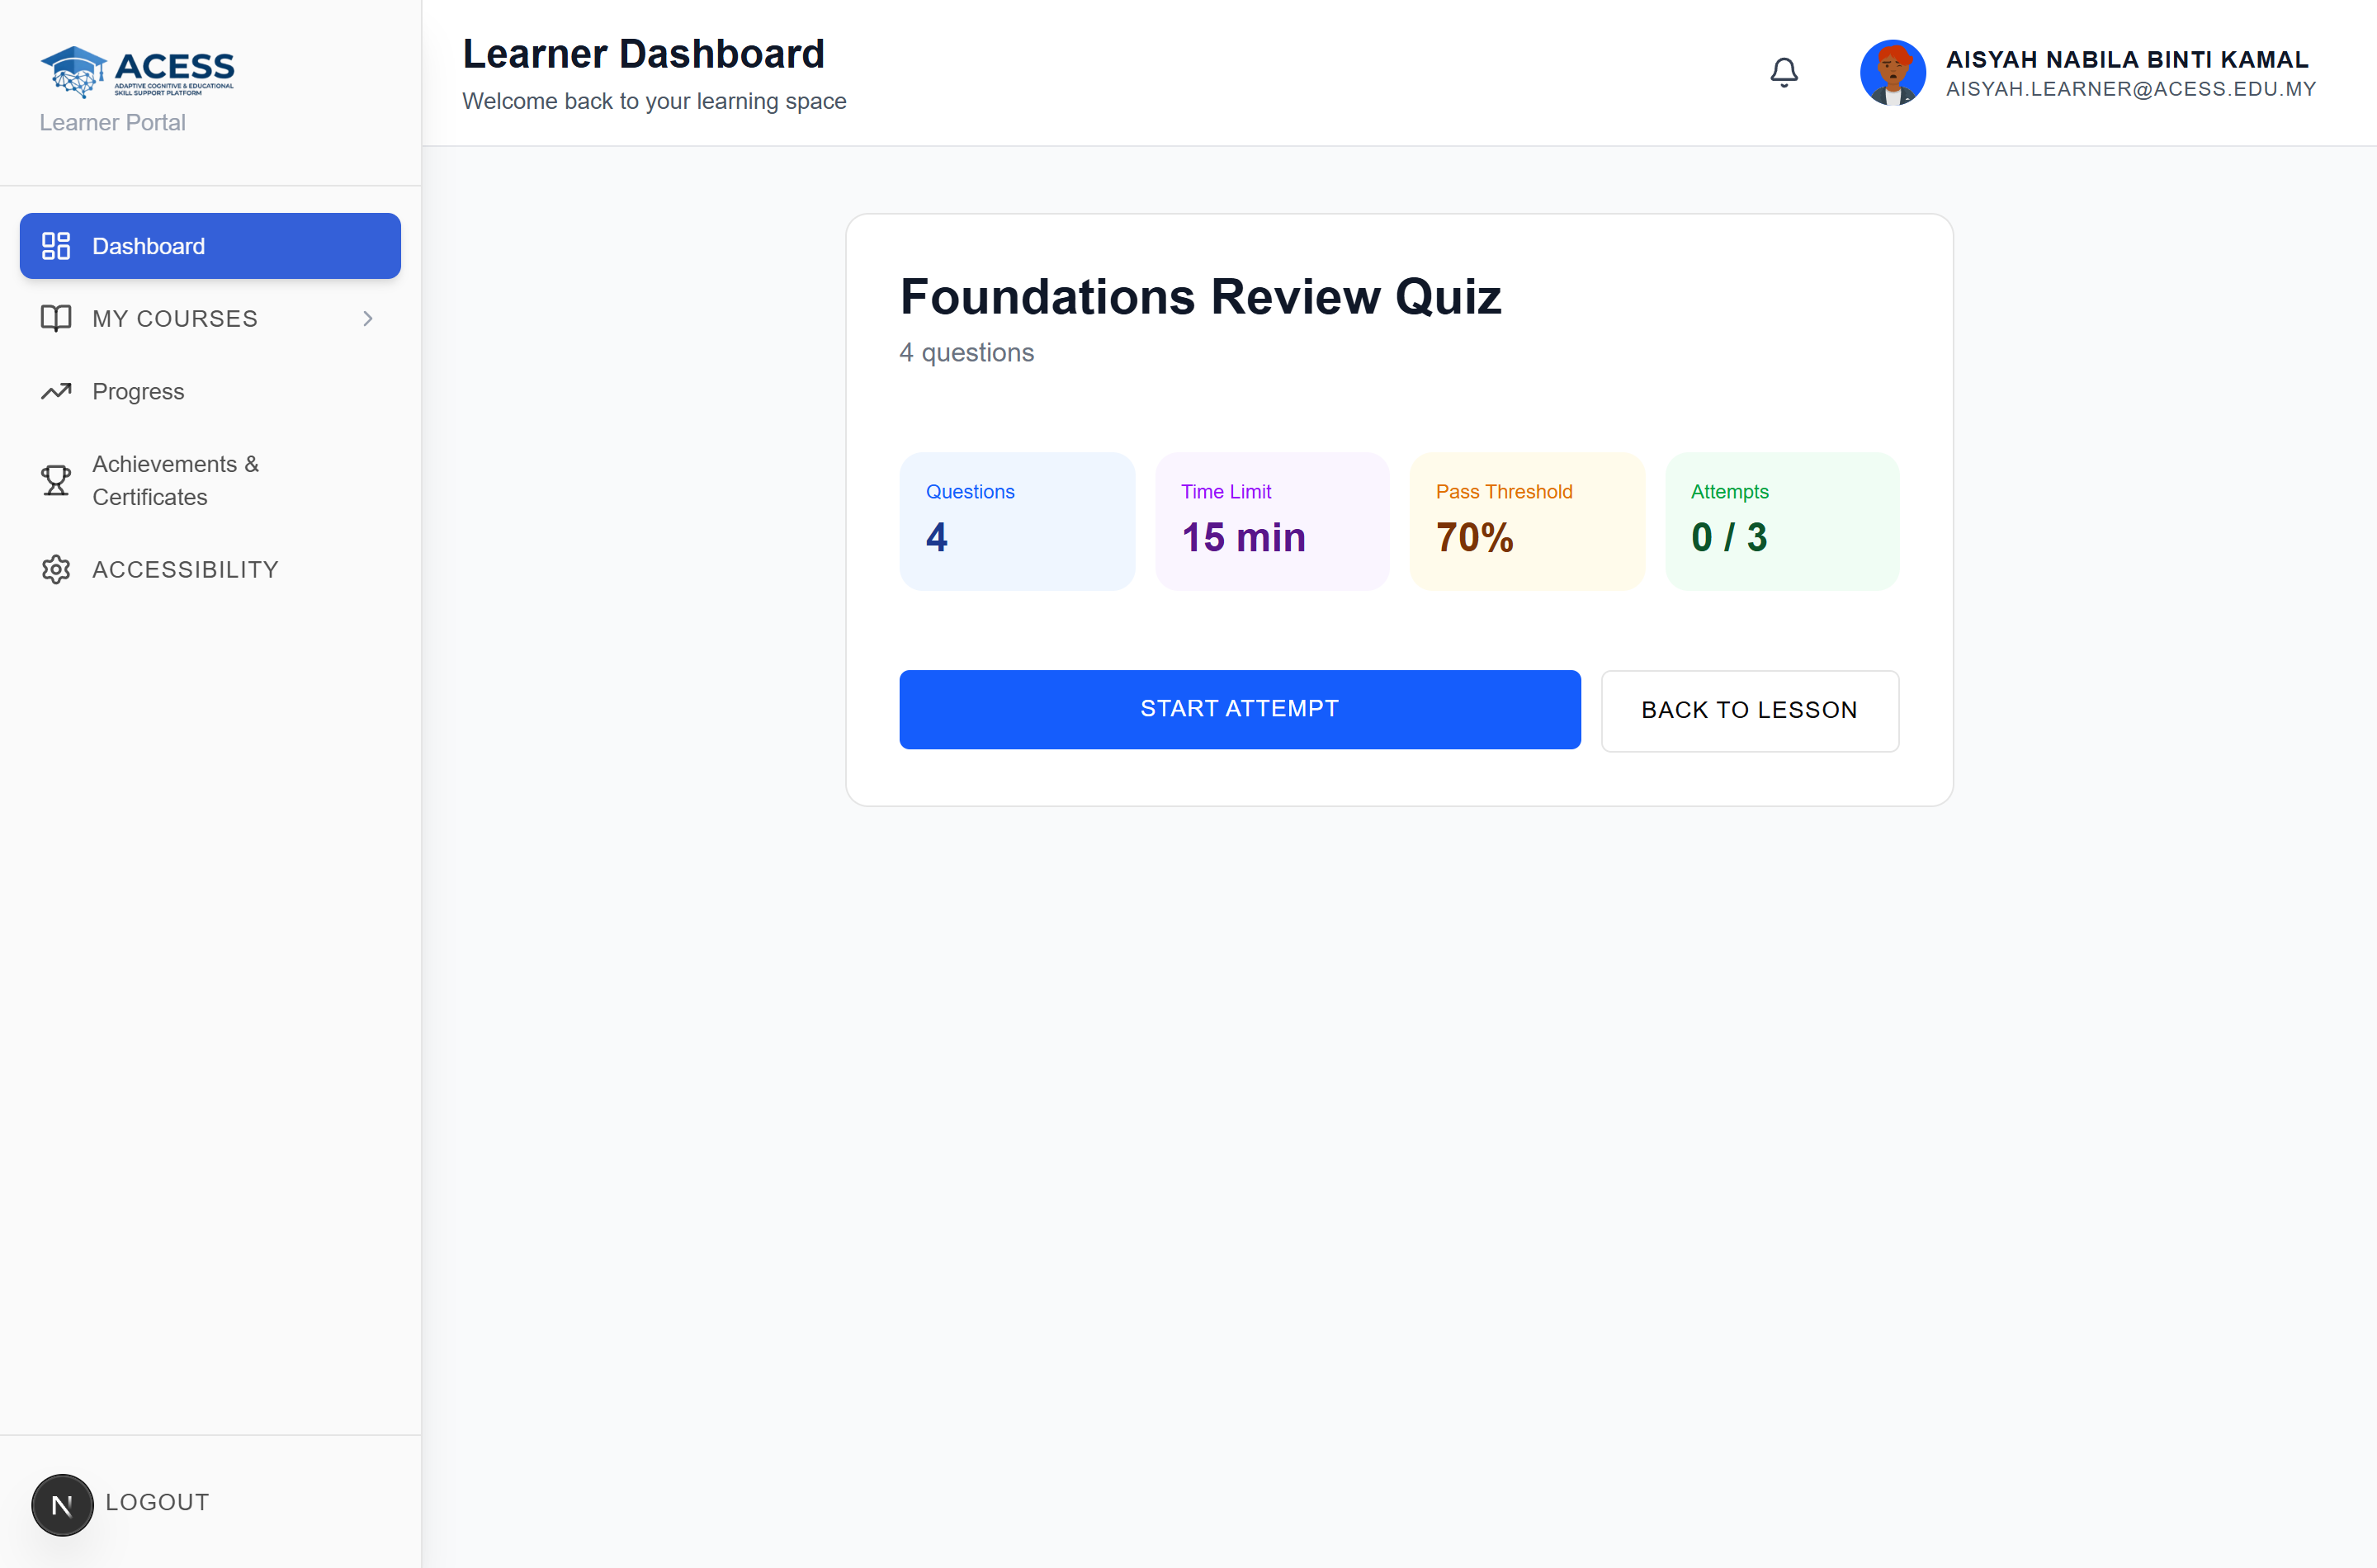
\includegraphics[width=0.92\textwidth]{Screenshots/learner-quiz.png}
\caption{Quiz Interface}
\label{fig:ui_quiz}
\end{figure}

\uidesignsub{Output Design}

Outputs fall into three classes: on-demand screen output, on-demand document output, and event-driven output. They are summarised below by the role each output serves.

\begin{itemize}
    \item \textbf{Public output.} The certificate verification page reports a certificate's validity, issue date and revocation status to anyone holding its reference code, without requiring an account.
    \item \textbf{Learner output.} A learner sees their own progress page (Figure~\ref{fig:ui_learner_progress}), receives event-driven notifications, and downloads a completion certificate once a course is finished.
    \item \textbf{Educator output.} An educator sees course analytics, the continuous accessibility compliance report described in Section~\ref{sec:a11y-audit}, and notifications on enrolment, quiz attempts and course publication.
    \item \textbf{Administrator output.} An administrator sees platform-wide analytics (Figure~\ref{fig:ui_admin_analytics}), including the accessibility-adaptation view unique to this platform (Figure~\ref{fig:ui_admin_a11y}), and generates a report as a PDF over a chosen date range.
\end{itemize}

Table~\ref{tab:output_design} then classifies every output above by its trigger basis, its audience and its content in full.

\begin{table}[H]
\caption{System Outputs}
\label{tab:output_design}
\vspace{-4mm}
\begin{center}
\renewcommand{\arraystretch}{1.2}
\footnotesize
\begin{tabular}{|>{\raggedright\arraybackslash\tabbreak}p{3.32cm}|>{\raggedright\arraybackslash\tabbreak}p{1.99cm}|>{\raggedright\arraybackslash\tabbreak}p{2.0cm}|>{\raggedright\arraybackslash\tabbreak}p{5.59cm}|}
\hline
\textbf{Output} & \textbf{Basis} & \textbf{Audience} & \textbf{Content} \\
\hline \hline
Learner progress page & Ad hoc & Learner & Course completion, lessons completed, study time, quiz history, visit history \\ \hline
Course analytics & Ad hoc & Educator & Enrolment and completion trends, per-lesson completion, quiz score distribution, at-risk flags \\ \hline
Platform analytics & Ad hoc & Admin & Registrations, enrolments, learning time, accessibility adaptation usage and preset adoption \\ \hline
Accessibility compliance report & Continuous & Educator & Per-lesson and per-course standards score, unmet rules, source of each rule \\ \hline
Administrator report (PDF) & Ad hoc & Admin & Platform, course, learner or content-coverage report over a chosen date range \\ \hline
Completion certificate (PDF) & Event & Learner & Learner name, course, completion date, reference code, verification QR code \\ \hline
Certificate verification page & Ad hoc & Public & Validity, issue date and revocation status for a reference code \\ \hline
Notifications & Event & All roles & Enrolment, lesson progress, quiz attempt, lesson added, course published \\ \hline
Achievement award & Event & Learner & Badge unlocked on meeting a course achievement's requirement \\ \hline
\end{tabular}
\end{center}
\end{table}

Figure~\ref{fig:ui_learner_progress} shows the learner-facing analytics output, with completion, study time and quiz telemetry for the signed-in learner, and Figure~\ref{fig:ui_admin_analytics} the administrator equivalent, with platform-level summary tiles and the registration trend series. Both are rendered with the same charting library, so that a figure carries the same visual grammar wherever it appears.

\begin{figure}[H]
\centering
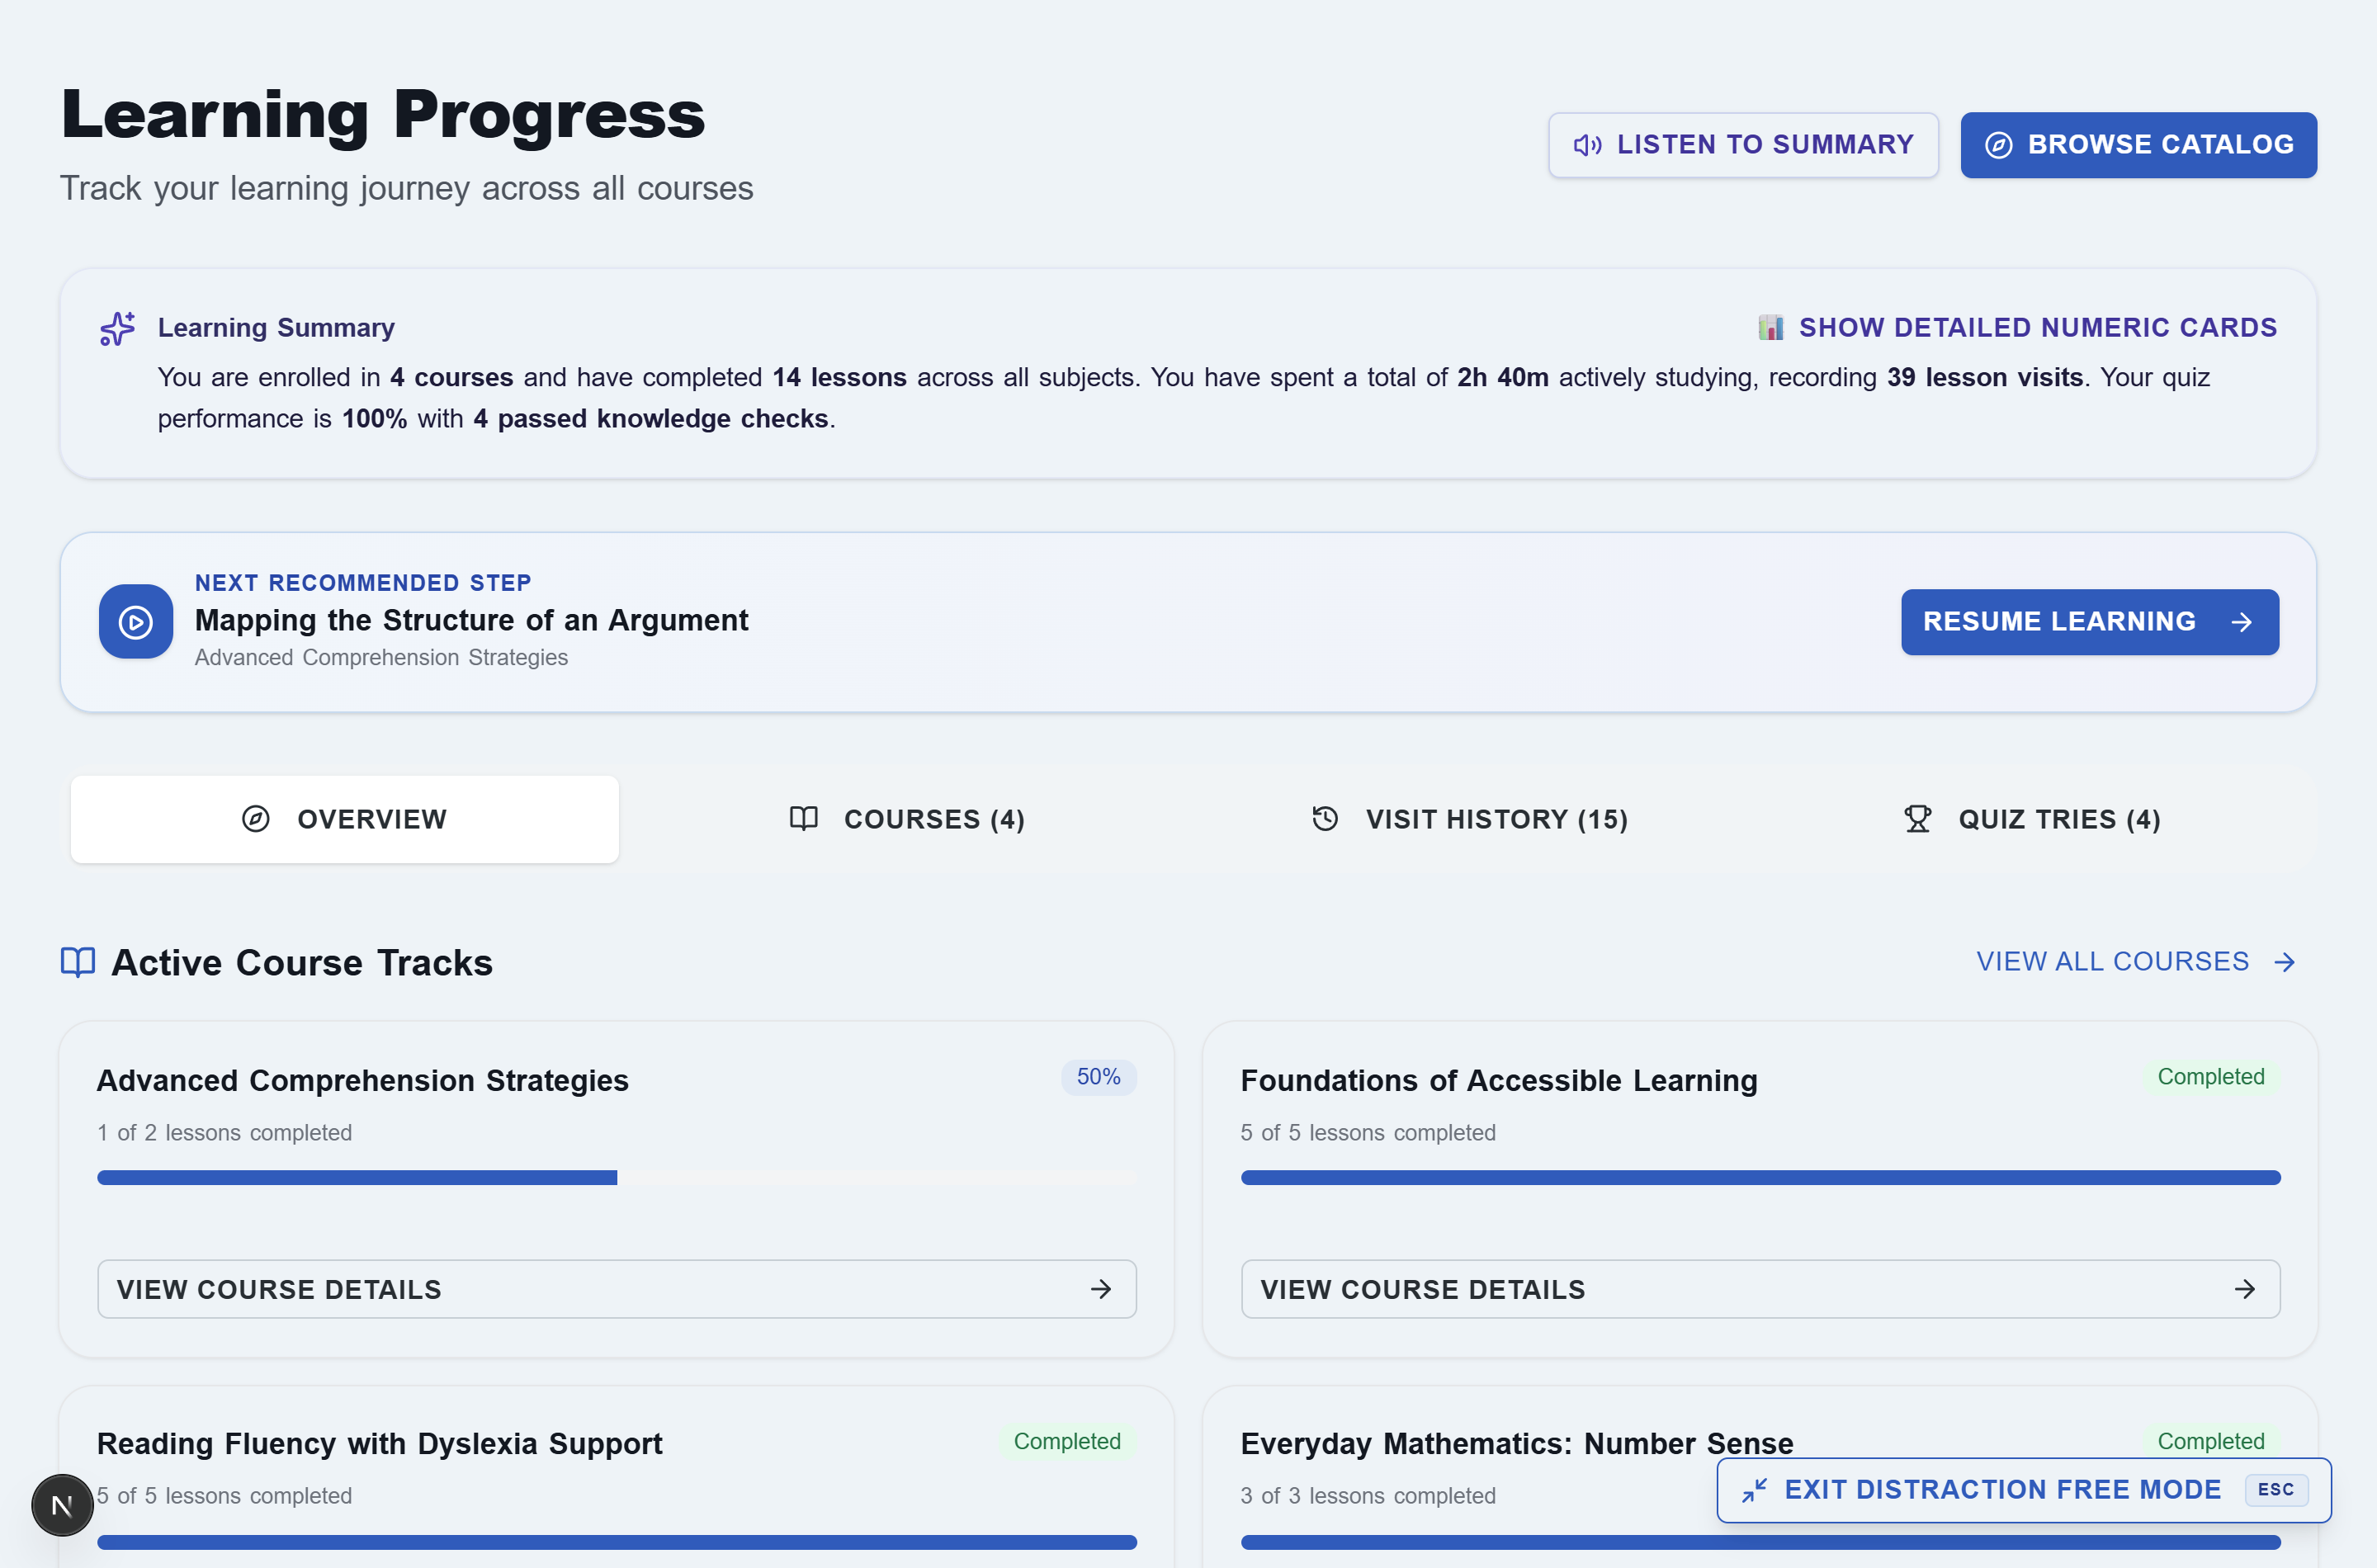
\includegraphics[width=0.92\textwidth]{Screenshots/learner-progress.png}
\caption{Learner Progress Page}
\label{fig:ui_learner_progress}
\end{figure}

\begin{figure}[H]
\centering
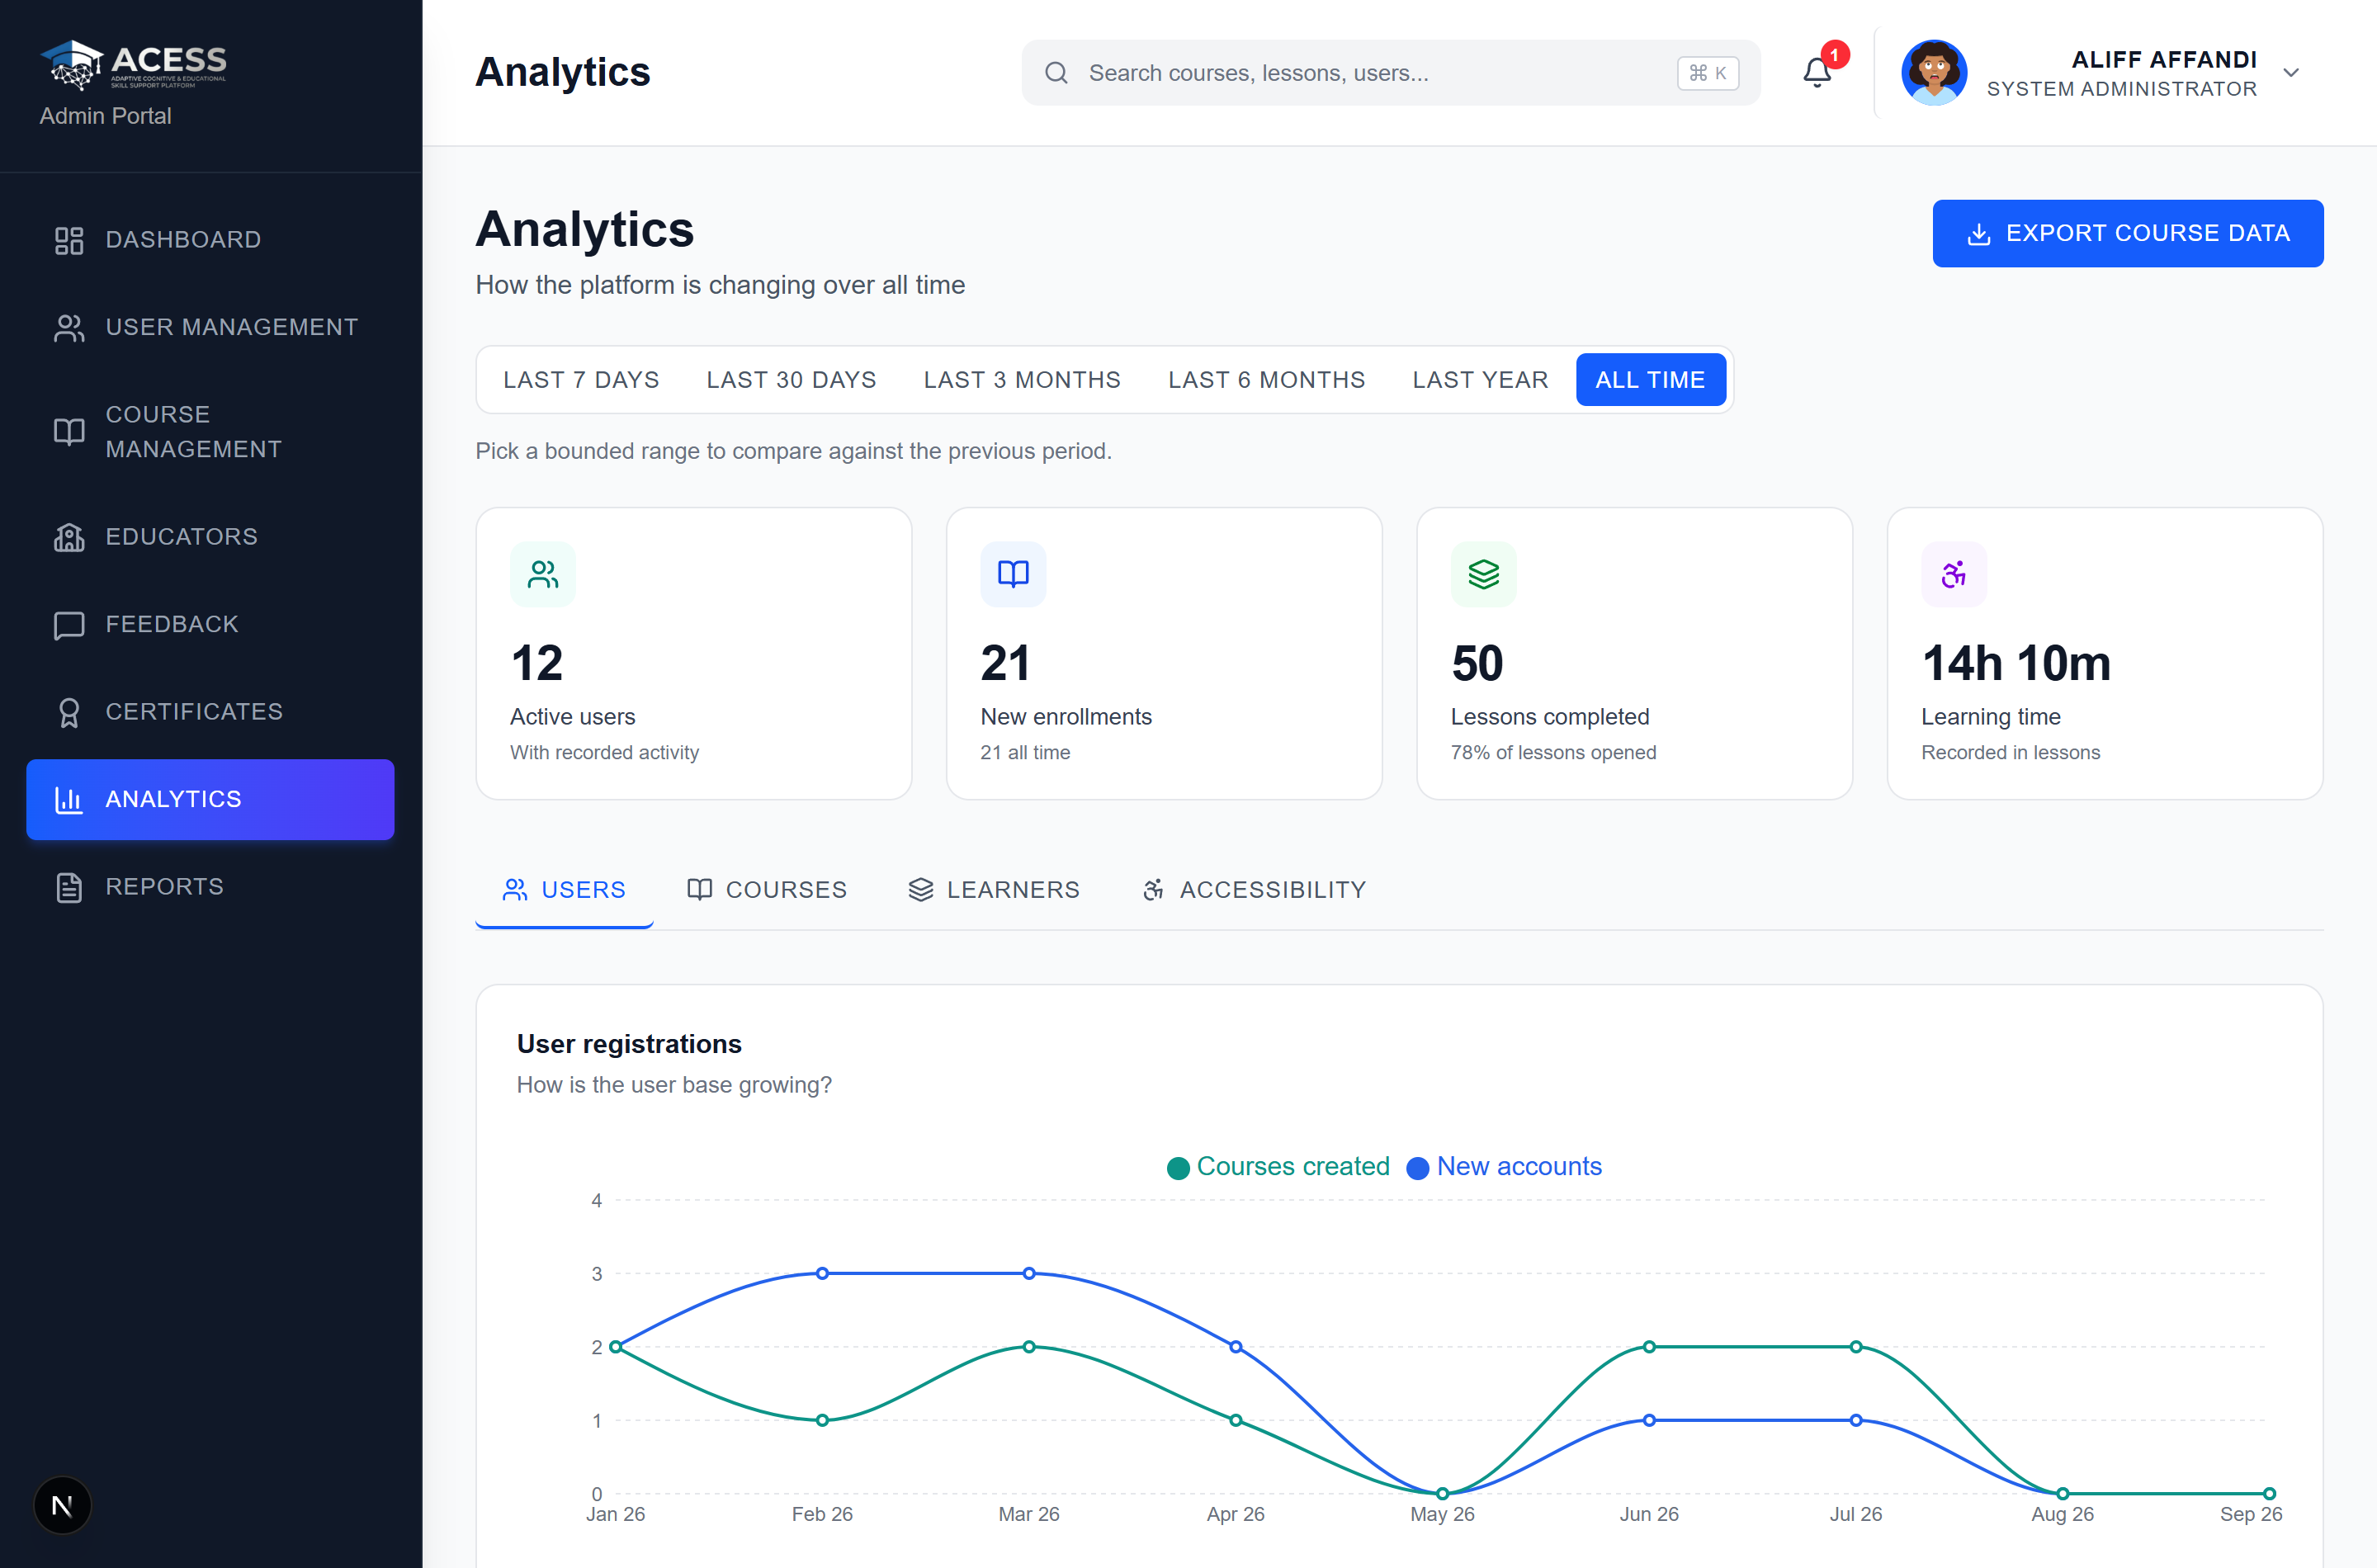
\includegraphics[width=0.92\textwidth]{Screenshots/admin-analytics.png}
\caption{Administrator Analytics Dashboard}
\label{fig:ui_admin_analytics}
\end{figure}

One output deserves separate mention because it is unusual in a learning platform. The administrator analytics view carries an Accessibility tab, shown in Figure~\ref{fig:ui_admin_a11y}, which reports which accessibility adaptations are actually being exercised and which presets learners actually choose, drawn from the platform's own adaptation-telemetry records. Accessibility features are frequently built and then never measured. This view exists so that the question ``is any of this being used?'' has an answer.

\begin{figure}[H]
\centering
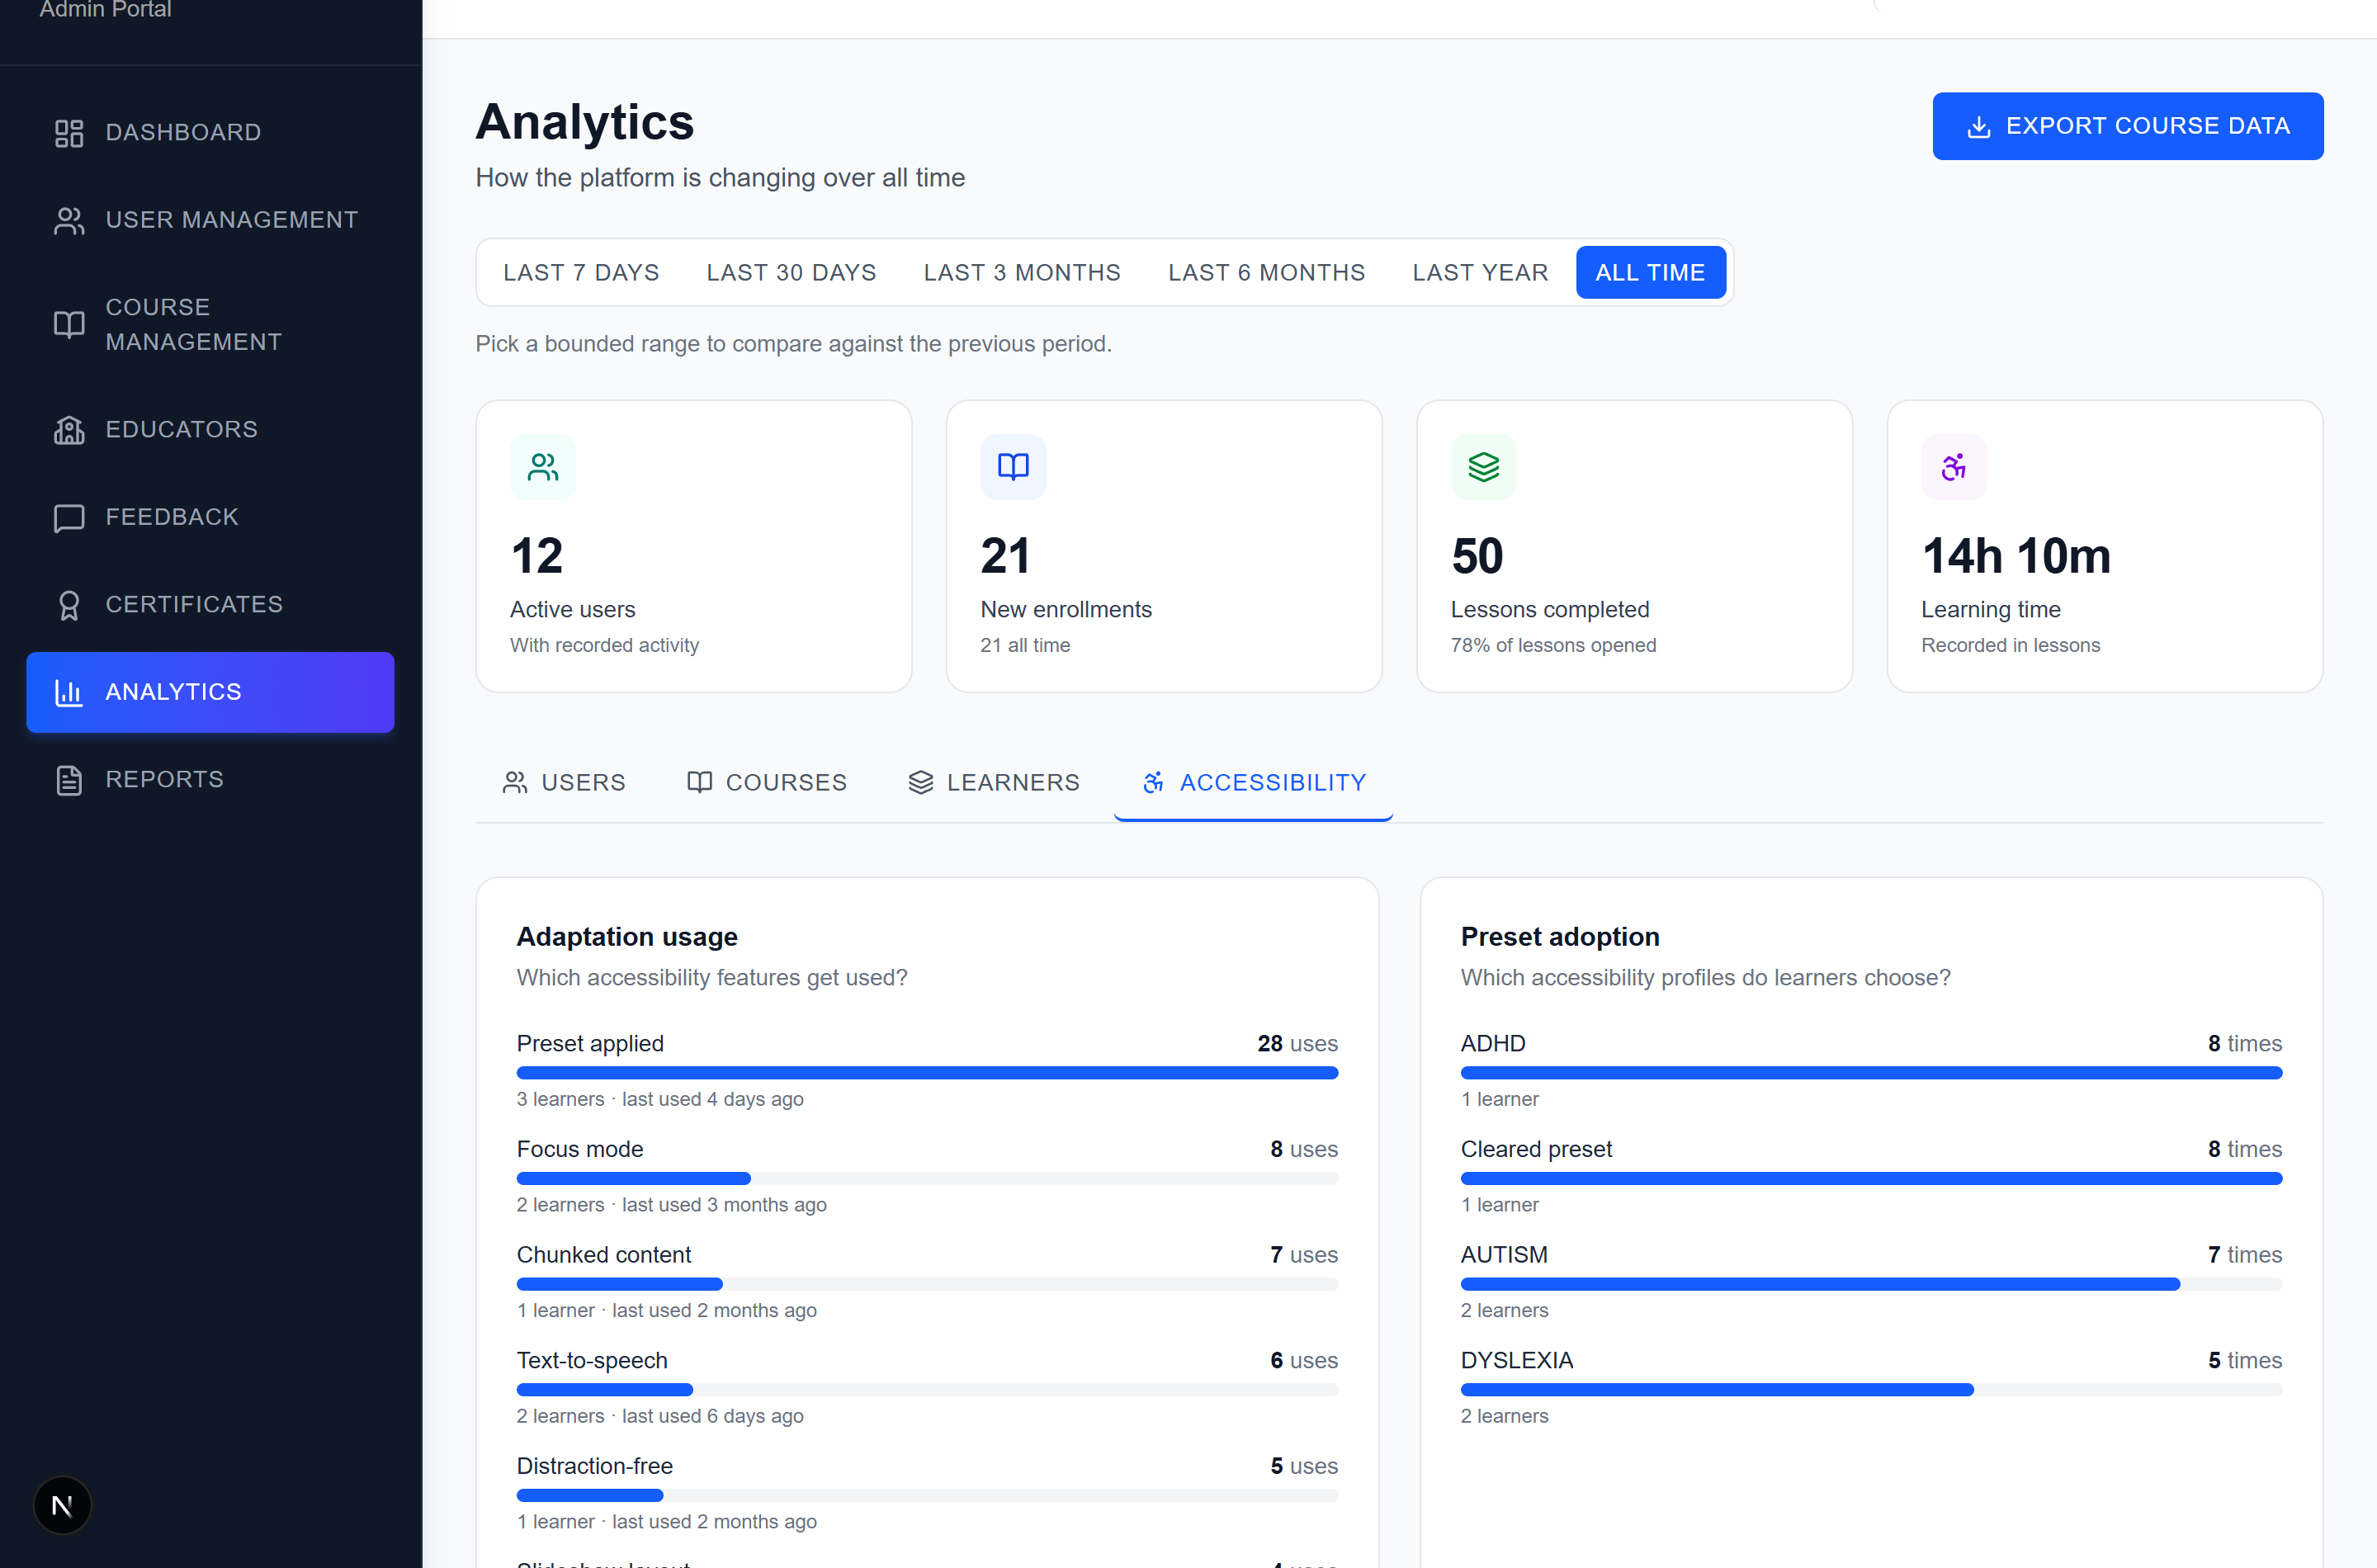
\includegraphics[width=0.92\textwidth]{Screenshots/admin-analytics-accessibility.png}
\caption{Accessibility Analytics}
\label{fig:ui_admin_a11y}
\end{figure}

\subsubsection{Conceptual and Logical Database Design}
\label{sec:erd}

The ACESS data model is a normalised relational schema implemented on PostgreSQL~17. In its current form it comprises \textbf{36 base tables, one view, 370 columns, 57 foreign keys, 33 check constraints, 20 unique constraints, 115 indexes, 20 functions, 15 triggers and 88 Row-Level Security policies}. These figures are not estimates: they were obtained by querying the system catalogues of a database rebuilt from the project's migrations, and the same query can be re-run to confirm them.

The Entity Relationship Diagrams in this section were likewise \emph{generated} from that live schema by a script in the repository (\tcode{scripts/erd-gen.mjs}) rather than drawn by hand, so that a diagram in this report cannot silently fall out of step with the database it claims to describe. Because thirty-six entities cannot be rendered legibly on a single portrait page, the model is presented as three domain diagrams, with the complete schema shown afterwards in landscape.

\paragraph{Business rules governing the relationships}

The following rules were derived from the platform's operational requirements and are what the foreign keys, unique constraints and delete rules in the schema encode.

\begin{enumerate}
    \item \textbf{One account, one identity record.} Every account has exactly one extended profile, and that profile is deleted automatically when the account is, because it holds nothing of value on its own.
    \item \textbf{A course must have an owner, and that owner cannot vanish.} Deleting the educator who owns a course is blocked outright. This is the only such restriction in the schema, and it is deliberate: removing an educator's account must not silently destroy the courses other people are enrolled in.
    \item \textbf{A learner enrols in a course at most once.} A uniqueness rule over the learner and course pair enforces this. Re-enrolment reactivates the existing enrolment rather than creating a second one, which is what keeps progress history continuous.
    \item \textbf{All learning activity hangs off the enrolment, not the learner.} Progress, quiz attempts, checkpoints, recommendations and certificates all reference the enrolment rather than the learner directly. This makes the enrolment the single unit of participation, so that withdrawing a learner from a course removes exactly that course's record and nothing else.
    \item \textbf{A lesson belongs to exactly one course, and optionally to one chapter.} The course link is mandatory. The chapter link is optional, because chapter organisation is a per-course feature an educator may switch on or leave off.
    \item \textbf{A lesson may declare one prerequisite lesson.} If that prerequisite is later deleted, the requirement is simply cleared rather than the dependent lesson breaking.
    \item \textbf{Assessment is strictly hierarchical.} A lesson has at most one quiz. A quiz has many questions. A question has many options, and exactly one option per question is flagged correct. An attempt records one answer per question, and an option that a submitted attempt still refers to cannot be deleted.
    \item \textbf{One certificate per enrolment.} A revoked certificate keeps its row and its reference code rather than being deleted, with its status changed to revoked. A check constraint enforces that a revoked record carries a revocation timestamp and an issued one does not, which is why public verification can report ``revoked'' rather than ``not found''.
    \item \textbf{An achievement is earned once per learner per course.} The record links the learner, the achievement definition and the course, and rows are inserted only by the platform's own derivation logic, never directly by a client.
    \item \textbf{Comments form a thread.} A comment may reference another comment as its parent, giving one level of reply nesting.
    \item \textbf{Accessibility state is per learner, not per enrolment.} A learner's presentation preferences follow them across every course, so they are stored on the learner's profile rather than on any individual enrolment.
\end{enumerate}

\paragraph{Domain 1: Identity, Access and Platform}

Figure~\ref{fig:erd_identity} shows the identity domain. It holds the account record, the extended profile that carries accessibility and notification preferences as JSON documents, the educator-application workflow, referral codes, platform notifications, the reusable accessibility content templates, and the adaptation telemetry that records which accessibility features are actually exercised. Every entity in this domain reaches \tcode{users} directly, which is why its policies are the simplest in the schema.

\begin{figure}[H]
\centering
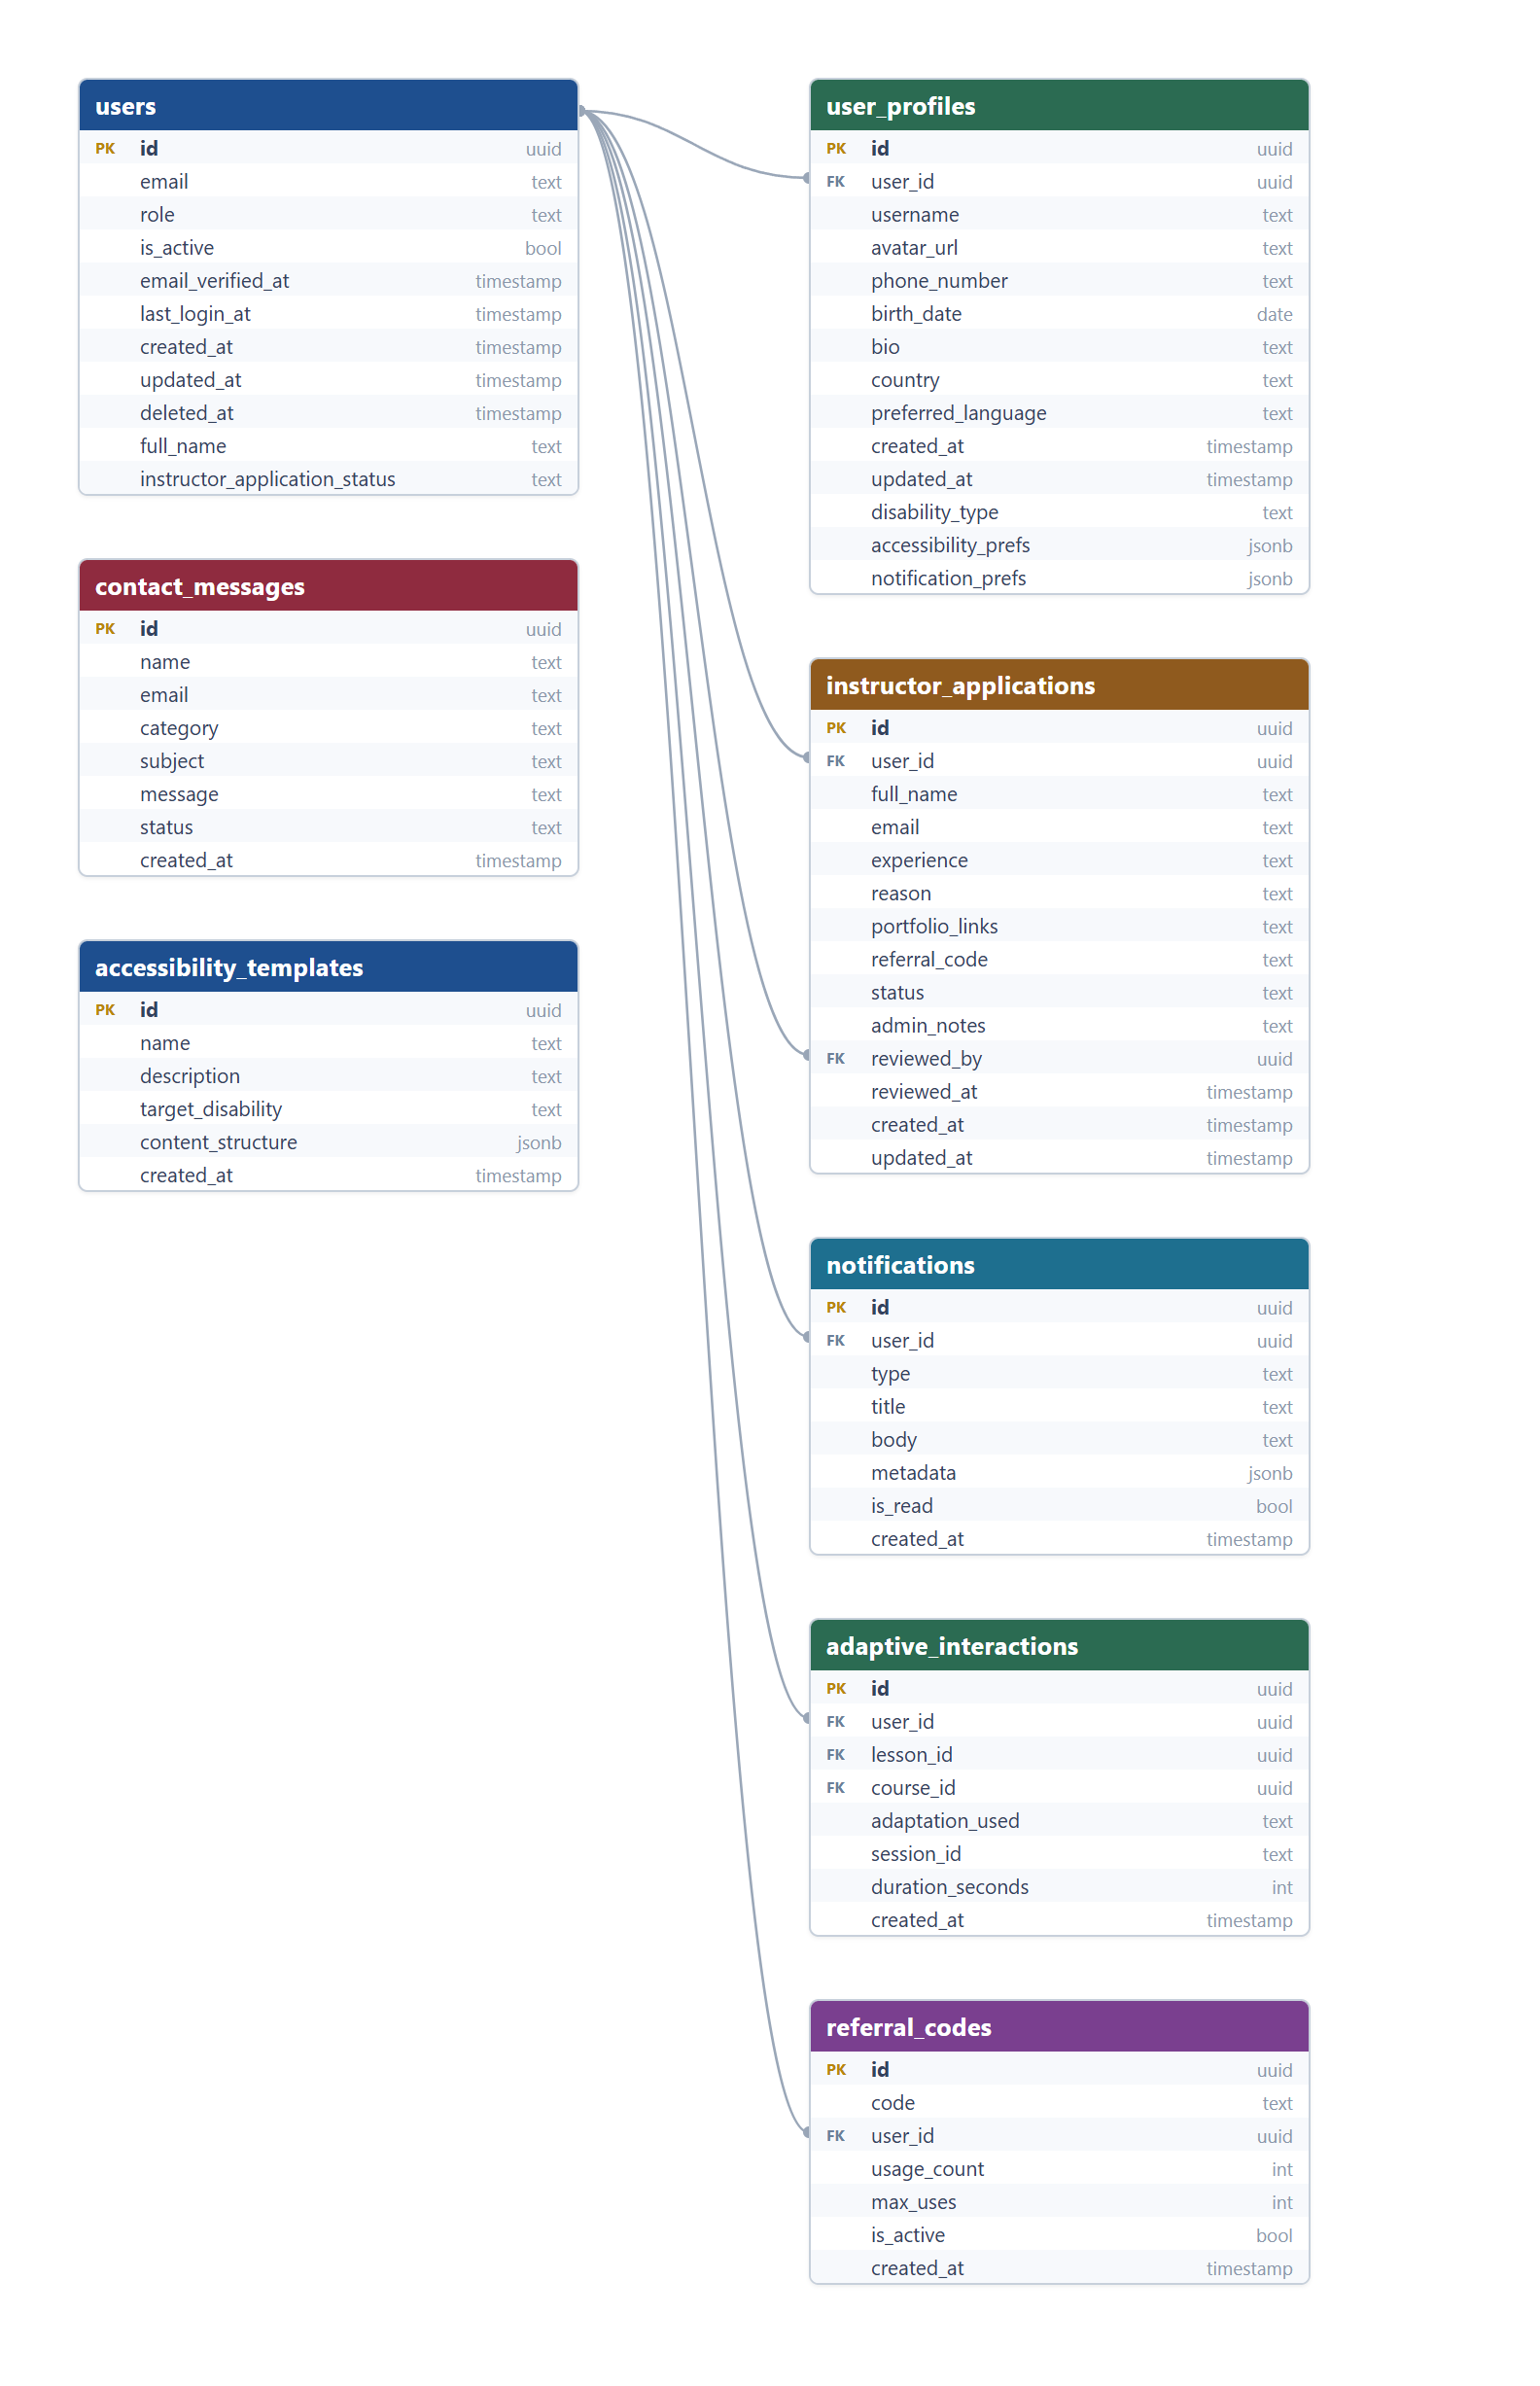
\includegraphics[width=\textwidth,height=0.84\textheight,keepaspectratio]{Diagram/ERD-1-identity.png}
\caption{Identity, Access and Platform ERD}
\label{fig:erd_identity}
\end{figure}

\paragraph{Domain 2: Curriculum and Content}

Figure~\ref{fig:erd_curriculum} shows the curriculum domain. It holds the course hierarchy (course, chapter, lesson), the authored artefacts attached to a lesson (interactive activities, in-video questions, H5P embeds, checkpoints, cached AI summaries and discussion threads), and the supporting content infrastructure of templates, version snapshots and uploaded media. Everything in this domain is authored by an educator, and nothing in it is generated by a learner.

\begin{figure}[H]
\centering
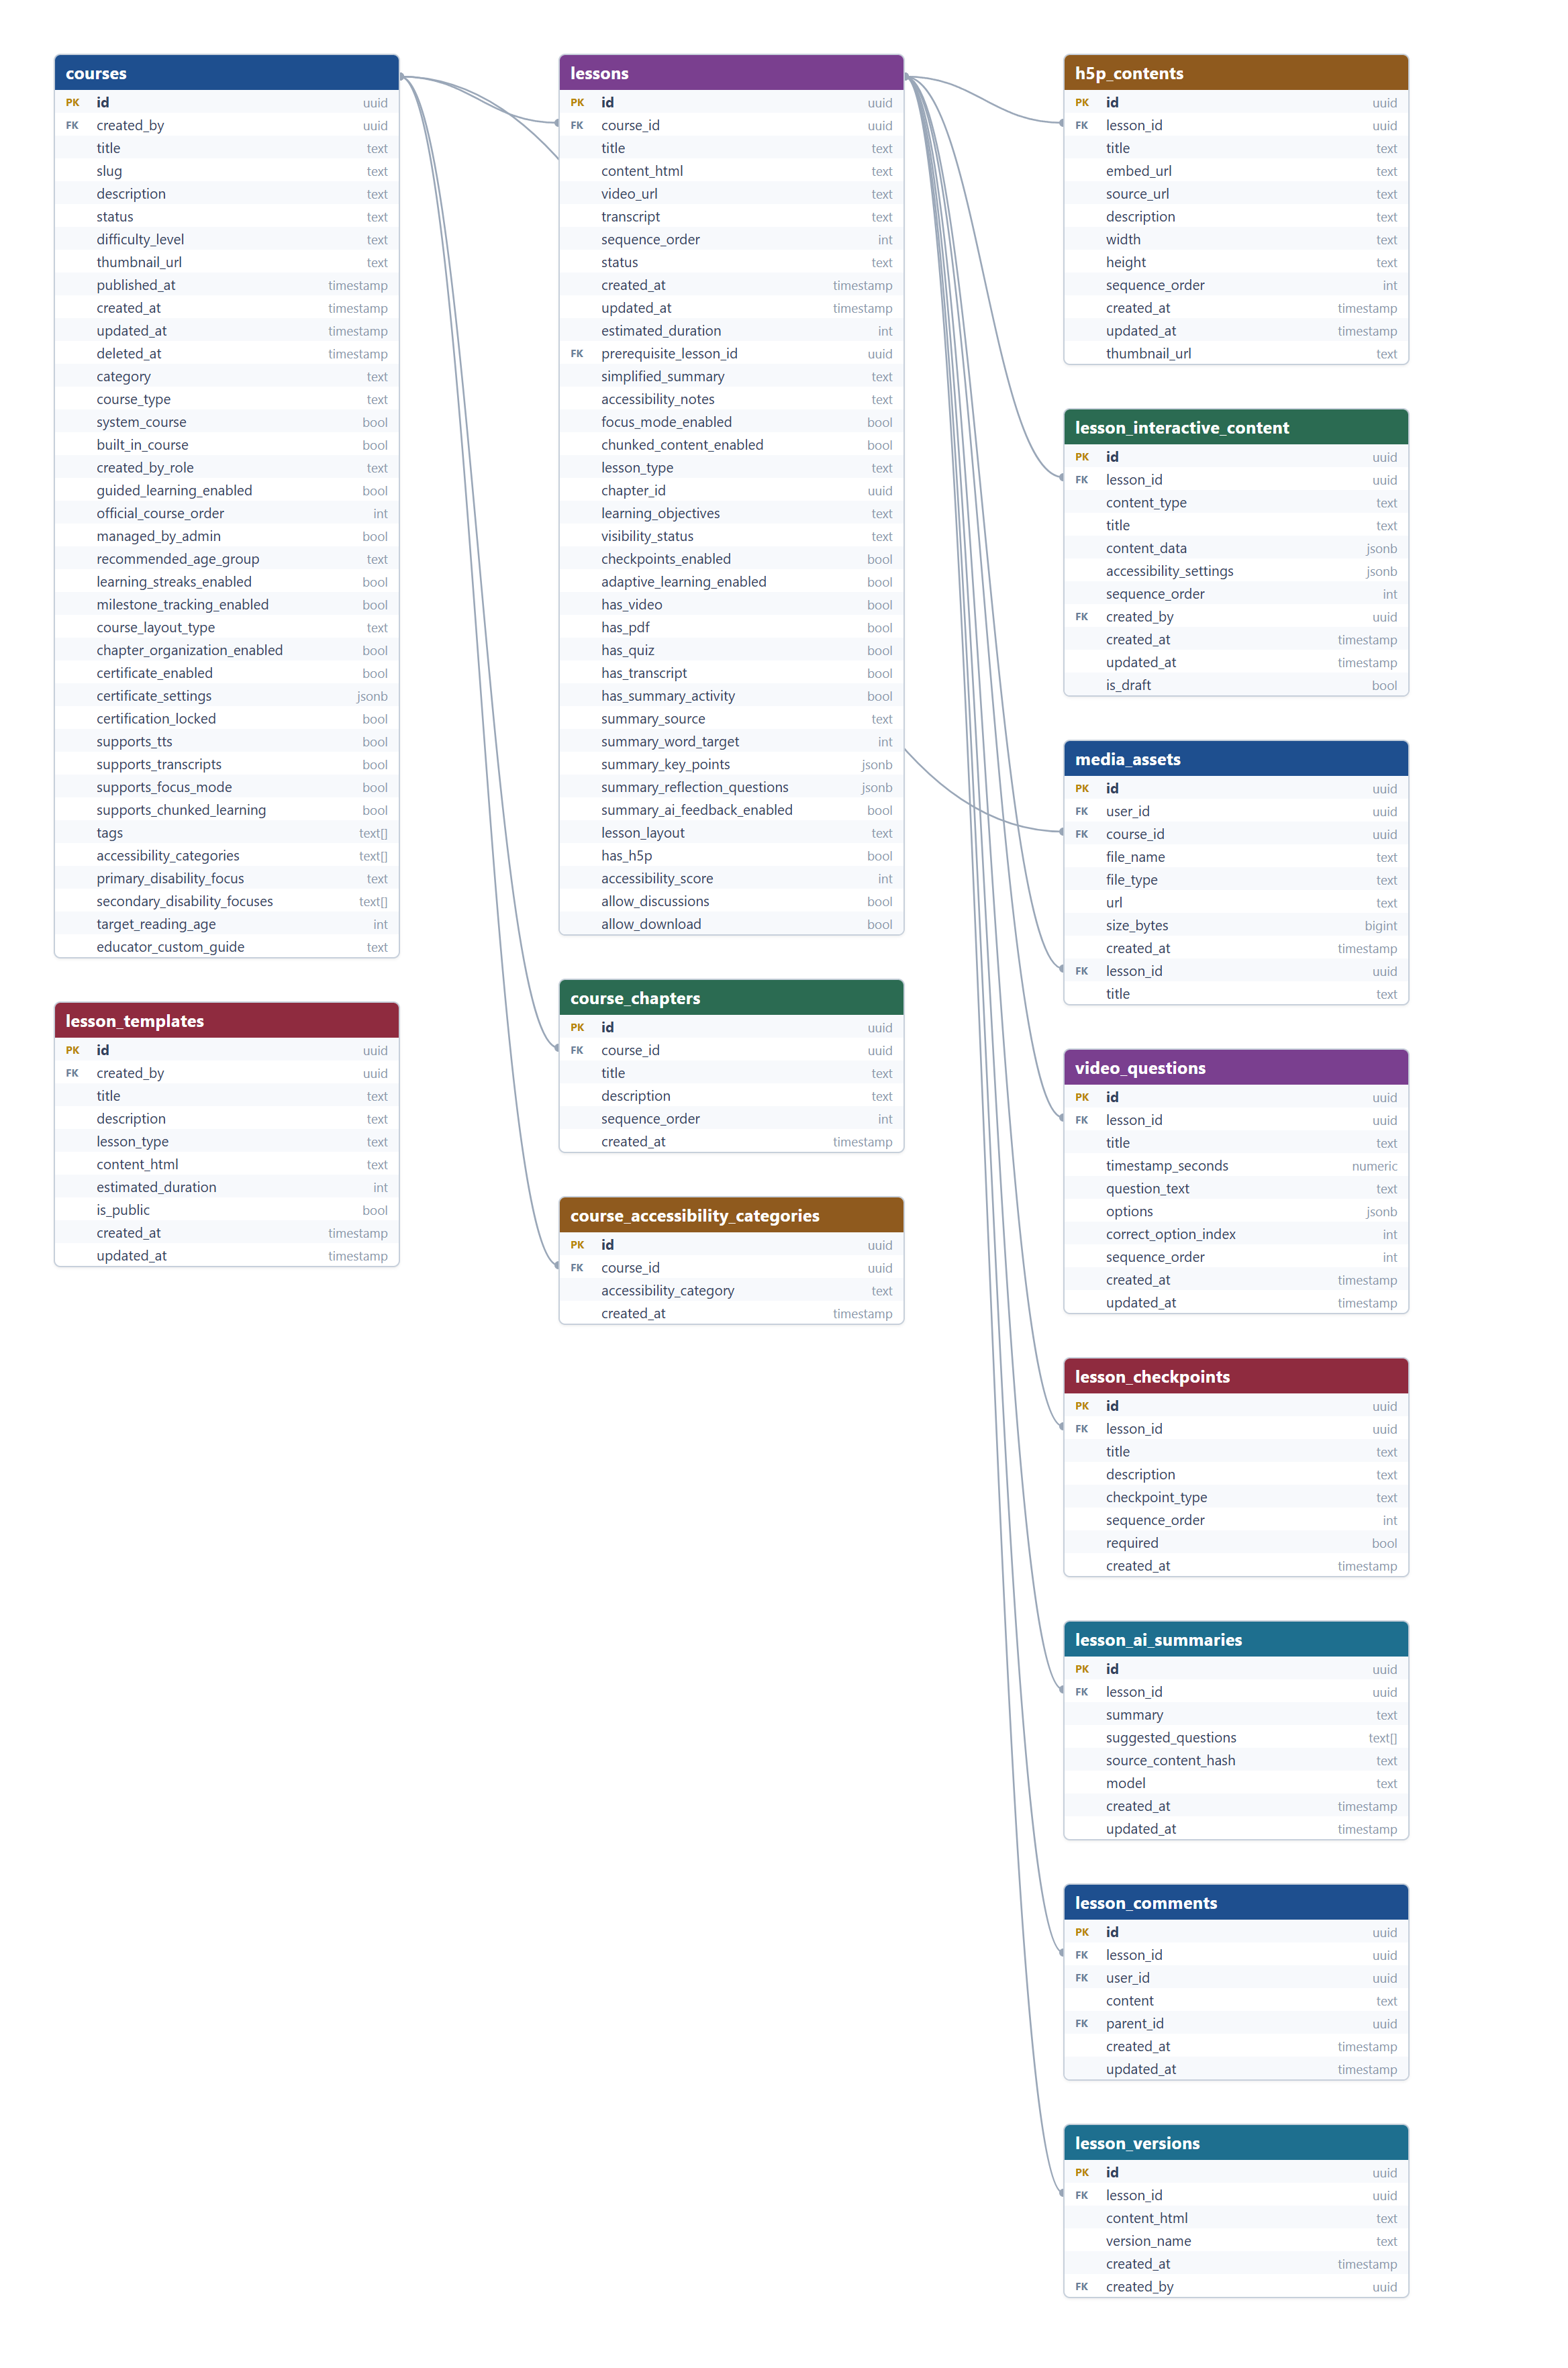
\includegraphics[width=\textwidth,height=0.84\textheight,keepaspectratio]{Diagram/ERD-2-curriculum.png}
\caption{Curriculum and Content ERD}
\label{fig:erd_curriculum}
\end{figure}

\paragraph{Domain 3: Assessment, Learning Record and Recognition}

Figure~\ref{fig:erd_assessment} shows the assessment and learning-record domain, which holds everything generated by a learner rather than authored by an educator: the enrolment itself, per-lesson progress, quiz attempts and answers, checkpoint responses, H5P responses, generated recommendations, favourites, and the recognition artefacts of achievements, milestones and certificates. The convergence of so many entities on \tcode{enrollments} is what business rule~4 above describes.

\begin{figure}[H]
\centering
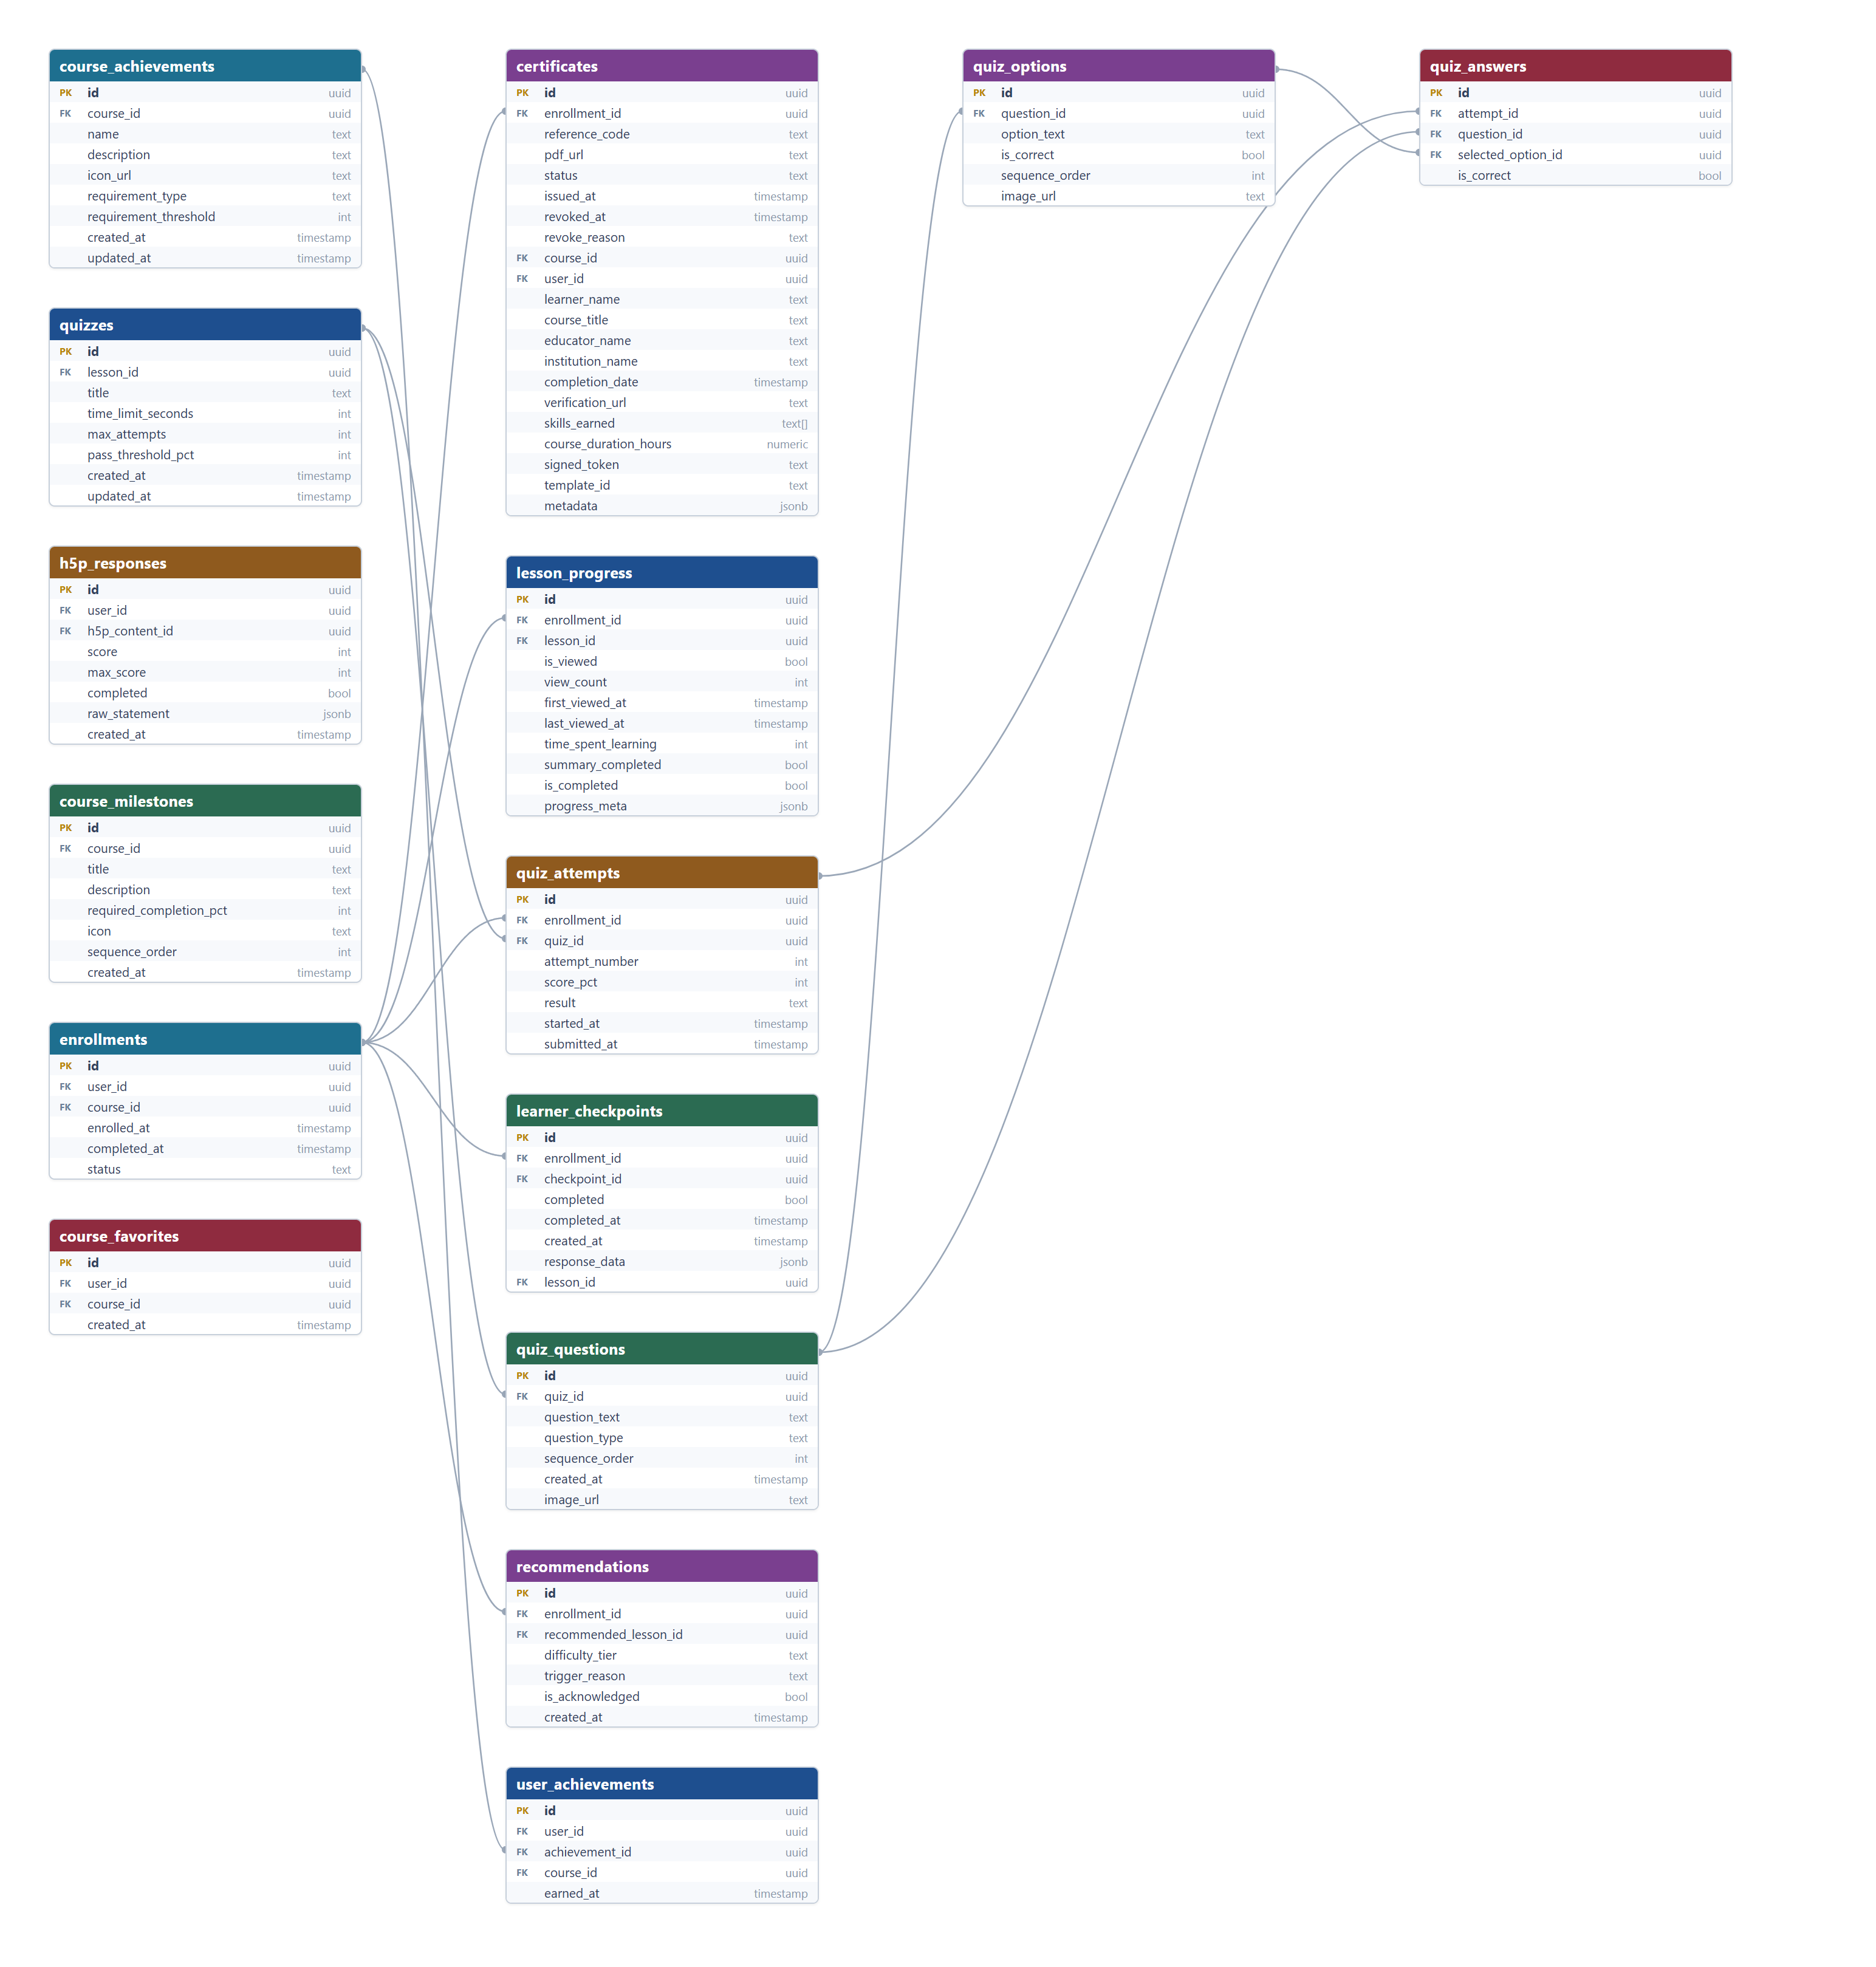
\includegraphics[width=\textwidth,height=0.84\textheight,keepaspectratio]{Diagram/ERD-3-assessment.png}
\caption{Assessment, Learning Record and Recognition ERD}
\label{fig:erd_assessment}
\end{figure}

\begin{landscape}
\begin{figure}[H]
\centering
% Explicit dimensions rather than \textwidth/\textheight: inside the rotated
% frame those two no longer correspond to the physical page edges, and using
% them shrank this diagram to roughly half the space actually available.
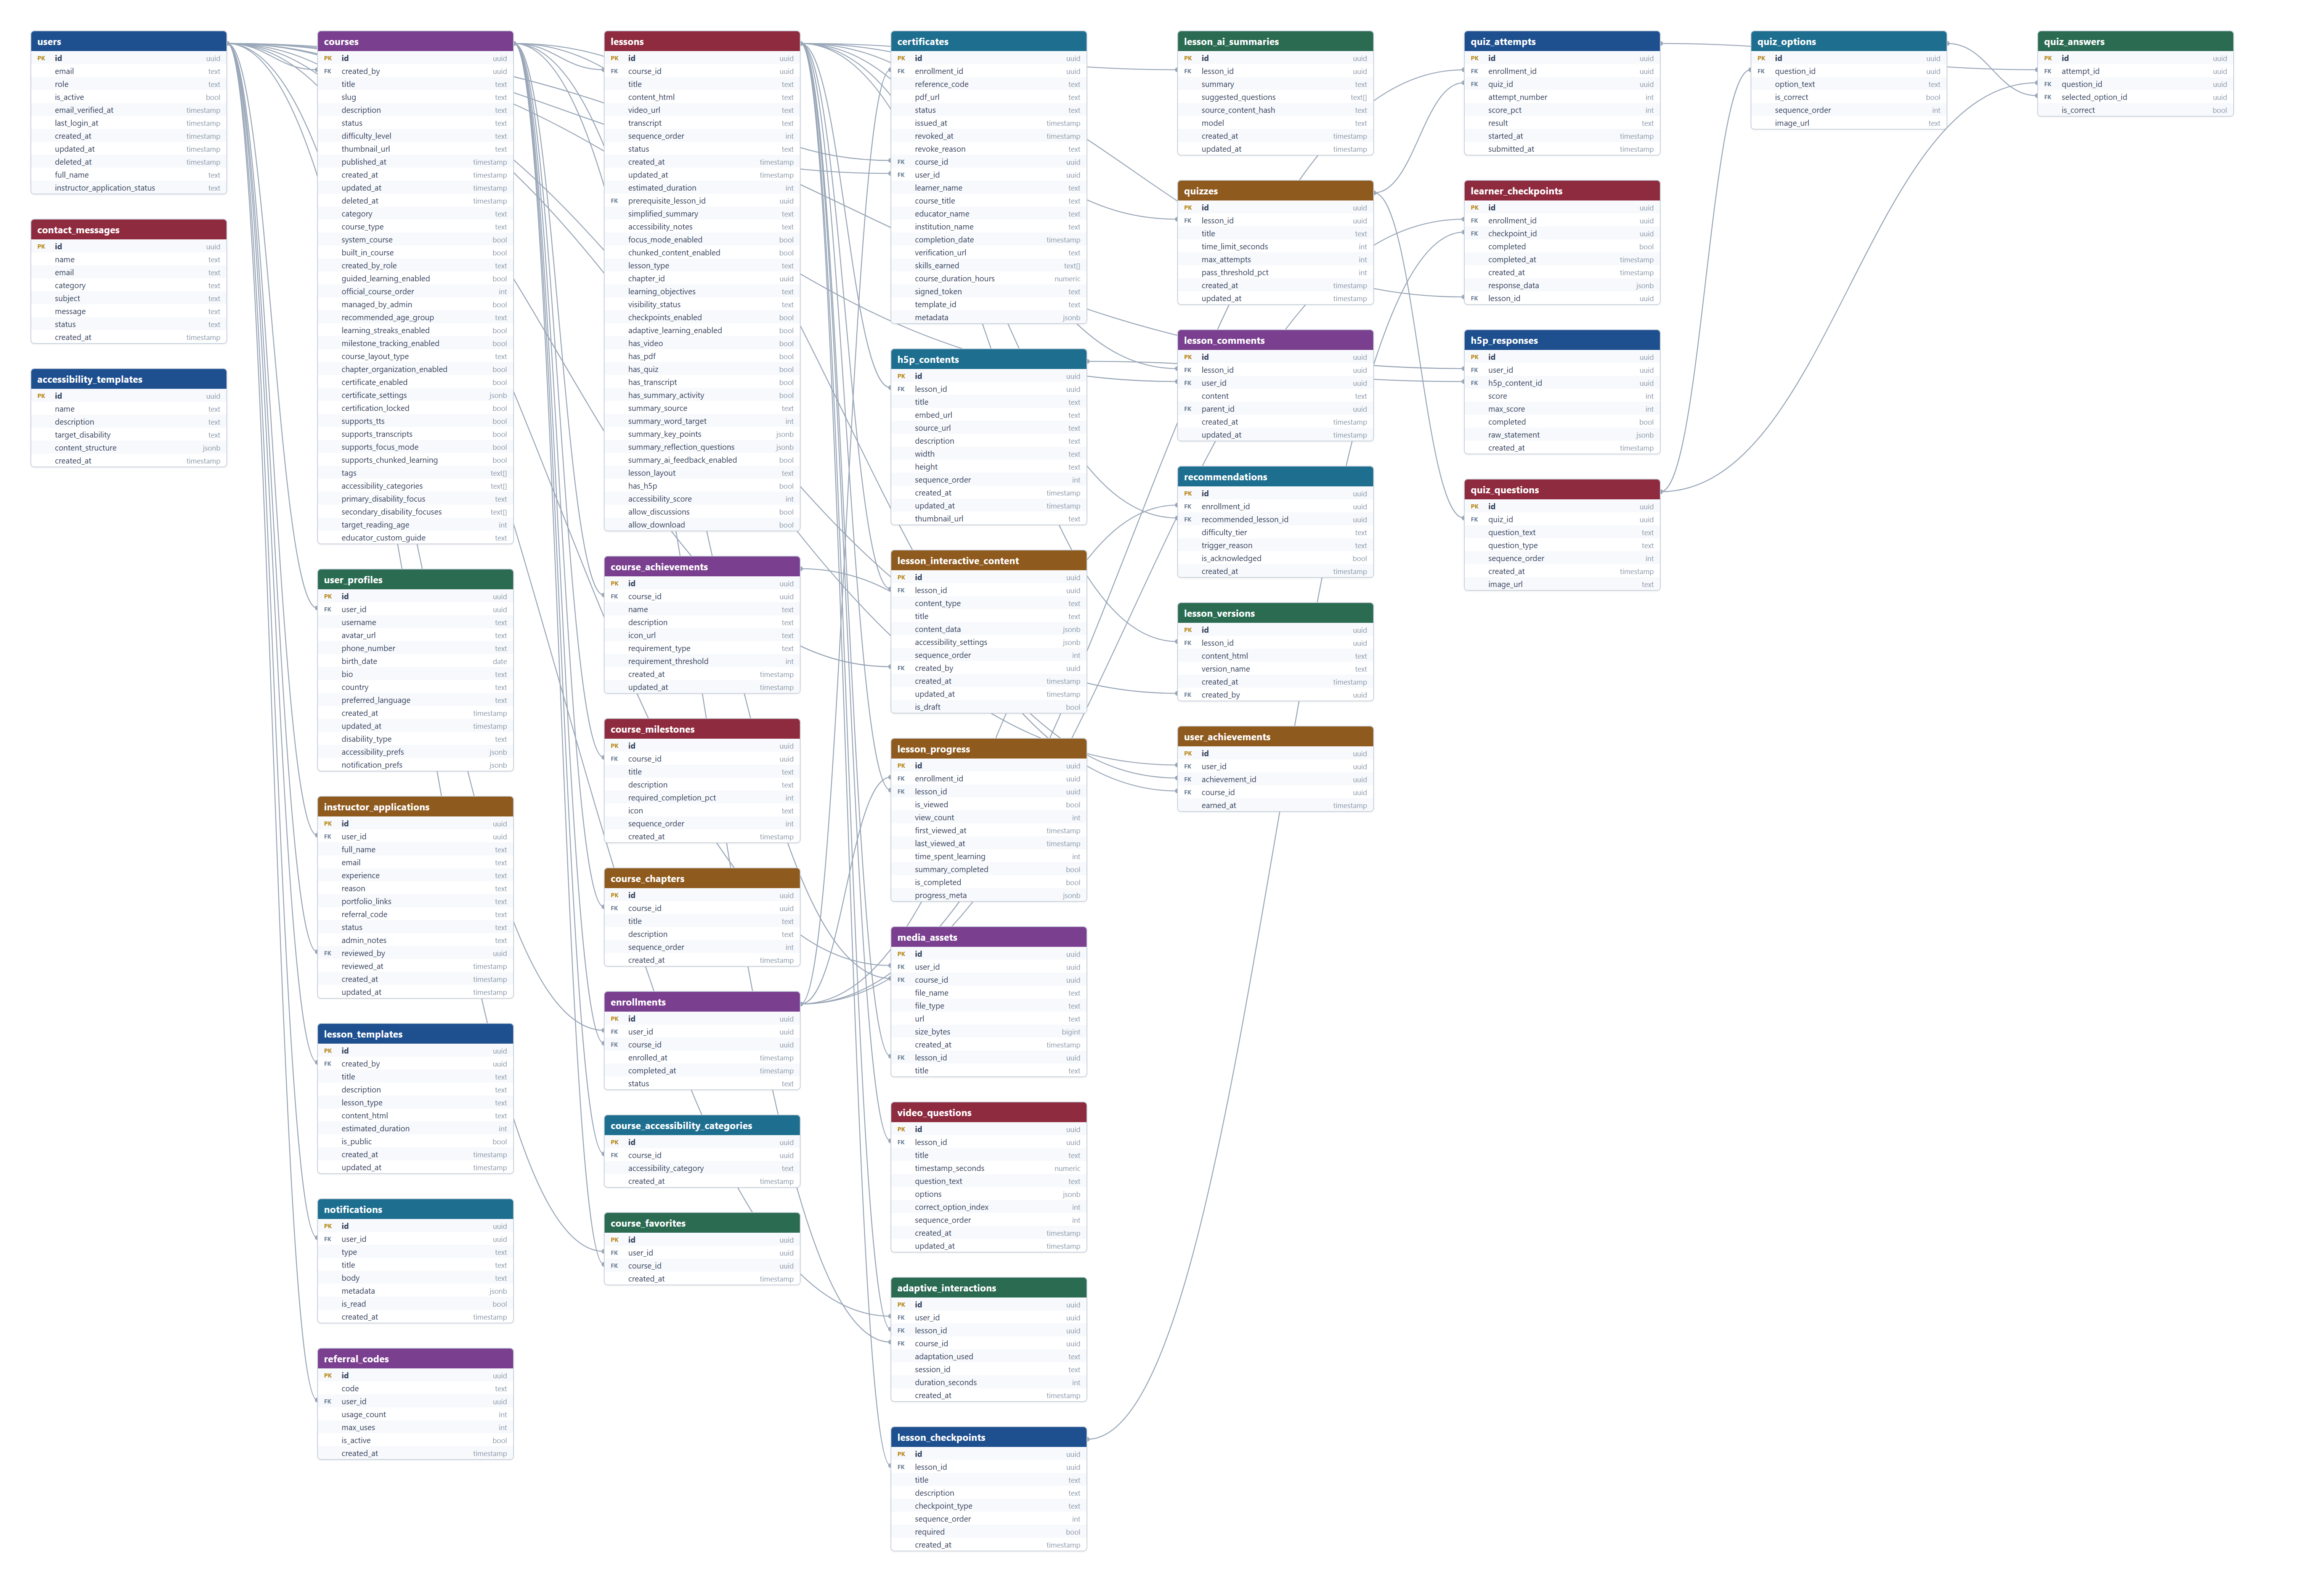
\includegraphics[width=20cm,height=13.3cm,keepaspectratio]{Diagram/ERD-0-overview.png}
\caption{Complete ACESS Entity Relationship Diagram}
\label{fig:erd}
\end{figure}
\end{landscape}

Figure~\ref{fig:erd} presents the full model, generated from all 36 tables and 57 foreign keys in the live schema. The \tcode{users} table acts as the identity hub and \tcode{enrollments} as the participation hub: nearly every learner-generated row reaches \tcode{users} through an enrolment rather than directly, which is what makes the row-level security policies expressible as a single join in most cases.

\subsection{Accessibility Design}
\label{sec:a11y-design}

\subsubsection{Design approach and standards baseline}

Accessibility in ACESS is not a settings panel bolted onto a finished product. It is the design constraint the rest of the system is arranged around. Three commitments follow from that, and they explain most of the design decisions in this section.

The first is that \textbf{a control must do what its label says}. During development a number of settings were found to be inert: a word-spacing slider that a stylesheet rule silently overrode, a line-spacing control that changed the settings preview but not the lesson, and an ``Easy Read'' mode that could not be reached from anywhere in the interface. Each of these was a control that appeared to work and did not. They were repaired, and the platform now maintains an explicit catalogue of every learner-facing setting, checked automatically, under an invariant stated in the project's own design documentation: if a setting is not in the catalogue, it does not exist. Two settings that still do not fully honour their labels are recorded as known gaps in Section~\ref{sec:a11y-gaps} rather than presented as working.

The second is that \textbf{the standards baseline has to be wider than WCAG}. WCAG 2.2 is necessary but was not written primarily for cognitive difference: it can tell an author that contrast is insufficient, but not that a paragraph is too long to re-enter after looking away. ACESS therefore works from three sources together: WCAG 2.2 \cite{wcag22} for testable technical criteria, the W3C's \emph{Making Content Usable for People with Cognitive and Learning Disabilities} \cite{wcag_cognitive} for cognitive design objectives, and the British Dyslexia Association Style Guide \cite{bda_style_guide} for typographic and prose thresholds.

The third is that \textbf{the claim must not exceed the evidence}. ACESS \emph{targets} WCAG 2.2 Level AA plus four Level AAA criteria. It has not been audited, has not been tested with a screen reader or other assistive technology, and has not been tested with disabled learners. That statement is published on the platform itself at \tcode{/accessibility-statement}, where a prospective learner can read it before investing time in the product, and it is repeated in Section~\ref{sec:a11y-gaps} of this report.

\subsubsection{Mapping of standards to implementation}

Table~\ref{tab:wcag_map} maps each addressed criterion to the ACESS feature that addresses it, the learner profile it primarily serves, and the module in which it is implemented. The final column names the figure in this report that shows it, where one exists.

{
\renewcommand{\arraystretch}{1.15}
\scriptsize
\begin{longtable}{|>{\raggedright\arraybackslash\tabbreak}p{2.0cm}|>{\raggedright\arraybackslash\tabbreak}p{3.6cm}|>{\raggedright\arraybackslash\tabbreak}p{1.3cm}|>{\raggedright\arraybackslash\tabbreak}p{3.6cm}|>{\raggedright\arraybackslash\tabbreak}p{1.75cm}|}
\caption{Accessibility Criteria Mapping}
\label{tab:wcag_map}\\
\hline
\textbf{Criterion} & \textbf{ACESS feature addressing it} & \textbf{Profile served} & \textbf{Implemented in} & \textbf{Evidence} \\
\hline \hline
\endfirsthead
\multicolumn{5}{l}{\footnotesize\itshape Table~\ref{tab:wcag_map} continued from the previous page}\\
\hline
\textbf{Criterion} & \textbf{ACESS feature addressing it} & \textbf{Profile served} & \textbf{Implemented in} & \textbf{Evidence} \\
\hline \hline
\endhead
\hline
\multicolumn{5}{r}{\footnotesize\itshape continued on the next page}\\
\endfoot
\endlastfoot
1.1.1 Non-text Content (A) & Lesson auditor requires alternative text on every image, and offers an inline field to supply it & All & \tcode{accessibility-audit.ts} & Fig.~\ref{fig:ui_edu_a11y} \\ \hline
1.2.1 Video-only (A) & Auditor treats a lesson with video and no transcript as a required failure & All & \tcode{accessibility-audit.ts}, \tcode{lessons.transcript} & Fig.~\ref{fig:ui_edu_a11y} \\ \hline
1.2.2 Captions (A) & Captions shown on video by default when the learner enables the setting & Hearing, slower processing & \tcode{AccessibilityProvider} & Fig.~\ref{fig:ui_a11y_modal} \\ \hline
1.3.1 Info and Relationships (A) & Auditor rejects empty paragraphs used as visual spacing and requires real headings & All & \tcode{accessibility-audit.ts} & Fig.~\ref{fig:ui_edu_a11y} \\ \hline
1.4.4 Resize Text (AA) & Font size adjustable 12--24\,px, applied as a CSS custom property with no reload & Dyslexia & \tcode{AccessibilityProvider} & Fig.~\ref{fig:ui_a11y_modal} \\ \hline
1.4.5 Images of Text (AA) & Auditor requires body content to be real text so that read-aloud can reach it & Dyslexia & \tcode{accessibility-audit.ts} & Fig.~\ref{fig:ui_edu_a11y} \\ \hline
1.4.8 Visual Presentation (AAA) & Reading measure bounded in character units (72 default, 62 Dyslexia, 66 ADHD) and retained when navigation chrome is hidden & Dyslexia, ADHD & \tcode{globals.css} (\tcode{--content-measure}) & Fig.~\ref{fig:preset_dyslexia} \\ \hline
1.4.12 Text Spacing (AA) & Line spacing 1.0--3.0 and word spacing reaching 0.2\,em, both learner-set, with the Dyslexia preset at the 0.16\,em floor & Dyslexia & \tcode{AccessibilityProvider} & Fig.~\ref{fig:preset_dyslexia} \\ \hline
2.2.1 Timing Adjustable (A) & An educator's quiz time limit is displayed but never triggers automatic submission & ADHD, Autism & \tcode{QuizPage.tsx} & Fig.~\ref{fig:ui_quiz} \\ \hline
2.2.4 Interruptions (AAA) & Distraction-free mode removes navigation and notification chrome during a lesson & ADHD & \tcode{globals.css}, \tcode{LessonViewPage.tsx} & Fig.~\ref{fig:preset_adhd} \\ \hline
2.2.6 Timeouts (AAA) & 15-minute inactivity timeout announced by a warning 30 seconds before it acts & All & \tcode{SessionTimeout.tsx} & N/A \\ \hline
2.3.3 Animation (AAA) & One animation-level control (normal / low / none) reduces or removes motion site-wide & Autism, ADHD & \tcode{AccessibilityProvider} & Fig.~\ref{fig:ui_a11y_modal} \\ \hline
2.4.4 Link Purpose (A) & Auditor flags non-descriptive link text such as ``click here'' & All & \tcode{accessibility-audit.ts} & Fig.~\ref{fig:ui_edu_a11y} \\ \hline
2.4.6 Headings and Labels (AA) & Auditor requires headings once a lesson passes 200 words & All & \tcode{accessibility-audit.ts} & Fig.~\ref{fig:ui_edu_a11y} \\ \hline
3.1.5 Reading Level (AAA) & Auditor computes a Flesch--Kincaid grade level and compares it with the course's declared target reading age \cite{kincaid1975derivation} & Dyslexia & \tcode{accessibility-audit.ts} & Fig.~\ref{fig:ui_edu_a11y} \\ \hline
3.2.3 Consistent Navigation (AA) & Identical shell and navigation order on every page of a role, and the auditor checks structural consistency between lessons of one course & Autism & \tcode{Sidebar.tsx}, \tcode{accessibility-audit.ts} & Fig.~\ref{fig:ui_learner_dashboard} \\ \hline
3.2.5 Change on Request (AAA) & A preset shows exactly what it will change before it changes it, read-aloud never starts by itself, and no media autoplays & All & \tcode{PresetDetailsDialog.tsx} & Fig.~\ref{fig:preset_diff} \\ \hline
4.1.2 Name, Role, Value (A) & Navigation built from real links carrying current-page state, and icon-only controls given accessible names and states & All & \tcode{Sidebar.tsx} and lesson header & Fig.~\ref{fig:ui_learner_dashboard} \\ \hline
COGA Obj. 3--5 & Chunked layout, per-section time estimates, visual schedule and step-by-step guidance & ADHD, Autism & \tcode{VisualSchedule.tsx}, \tcode{StepByStepGuidance.tsx} & Fig.~\ref{fig:preset_autism} \\ \hline
\end{longtable}
}

Table~\ref{tab:wcag_map} makes one structural point about the design worth drawing out. The criteria divide cleanly into two groups by \emph{who} can satisfy them. Presentation criteria (1.4.4, 1.4.8, 1.4.12, 2.3.3, 2.2.6, 3.2.5) are satisfied by the platform, once, for everyone. Content criteria (1.1.1, 1.2.1, 1.3.1, 2.4.4, 2.4.6, 3.1.5) cannot be satisfied by the platform at all, because they are properties of what an educator writes. A platform can only make the requirement visible at the moment of writing, which is precisely what the compliance auditor described in Section~\ref{sec:a11y-audit} exists to do.

\subsubsection{The three learner profiles}

Table~\ref{tab:profiles} states, for each of the three profiles the platform is designed around, the accessibility needs it addresses and the concrete support ACESS provides. Every entry in the third column corresponds to code that runs. Nothing in it is aspirational.

{
\renewcommand{\arraystretch}{1.15}
\scriptsize
\begin{longtable}{|>{\raggedright\arraybackslash\tabbreak}p{1.51cm}|>{\raggedright\arraybackslash\tabbreak}p{5.0cm}|>{\raggedright\arraybackslash\tabbreak}p{6.99cm}|}
\caption{Learner Profiles and ACESS Support}
\label{tab:profiles}\\
\hline
\textbf{Profile} & \textbf{Main accessibility needs} & \textbf{ACESS support} \\
\hline \hline
\endfirsthead
\multicolumn{3}{l}{\footnotesize\itshape Table~\ref{tab:profiles} continued from the previous page}\\
\hline
\textbf{Profile} & \textbf{Main accessibility needs} & \textbf{ACESS support} \\
\hline \hline
\endhead
\hline
\multicolumn{3}{r}{\footnotesize\itshape continued on the next page}\\
\endfoot
\endlastfoot
Dyslexia &
\begin{tabular}[t]{@{}p{4.7cm}@{}}
\textbullet\ Reduced decoding effort \\
\textbullet\ Reduced visual crowding between letters, words and lines \\
\textbullet\ A reliable way not to lose one's place in a long passage \\
\textbullet\ An alternative to reading \\
\textbullet\ Reduced glare over long sessions
\end{tabular} &
\begin{tabular}[t]{@{}p{6.7cm}@{}}
\textbullet\ Atkinson Hyperlegible or OpenDyslexic typeface, 19\,px base size, 1.7 line spacing \\
\textbullet\ Word spacing at the 0.16\,em WCAG floor \\
\textbullet\ Reading measure narrowed to 62 characters (the BDA recommends 50--70) \\
\textbullet\ Cream background, and a reading spotlight that dims all but the current paragraph \\
\textbullet\ Text-to-speech with adjustable rate and a click-to-read-from-here control \\
\textbullet\ A dedicated reading toolbar carrying size, spacing, tint and spotlight controls without leaving the lesson \\
\textbullet\ Italic rendered as bold rather than slanted, text never justified \\
\textbullet\ Content presented one section at a time, on a single-column dashboard rather than a card grid
\end{tabular} \\ \hline
ADHD &
\begin{tabular}[t]{@{}p{4.7cm}@{}}
\textbullet\ Sustained attention is costly \\
\textbullet\ Task initiation is hard \\
\textbullet\ An interruption destroys one's place \\
\textbullet\ Passive reading does not retain \\
\textbullet\ Competing on-screen elements all pull equally
\end{tabular} &
\begin{tabular}[t]{@{}p{6.7cm}@{}}
\textbullet\ Distraction-free mode hiding sidebar and notification chrome \\
\textbullet\ Reading measure held at 66 characters, \emph{including} while chrome is hidden \\
\textbullet\ A persistent ``Now'' bar carrying the single current task and its progress \\
\textbullet\ A task checklist and a progress timeline \\
\textbullet\ An auto-save indicator so that leaving the page carries no risk \\
\textbullet\ Reading spotlight \\
\textbullet\ Content chunked into sections with a per-section reading-time estimate
\end{tabular} \\ \hline
& &
On the authoring side, the auditor caps a lesson at 20 minutes, an unbroken block at 150 words, expects a section break roughly every 400 words, expects video under six minutes or in-video questions, and requires at least one thing to \emph{do} in every lesson. \\ \hline
Autism &
\begin{tabular}[t]{@{}p{4.7cm}@{}}
\textbullet\ Uncertainty about what is coming is itself a barrier \\
\textbullet\ Sensory input can overload \\
\textbullet\ Figurative language must be decoded before content can be \\
\textbullet\ Inconsistent structure has to be re-learned every time
\end{tabular} &
\begin{tabular}[t]{@{}p{6.7cm}@{}}
\textbullet\ A visual schedule listing every phase of the lesson, with progress, \emph{before} the learner starts \\
\textbullet\ Step-by-step guidance that always states why a ``Next'' control is unavailable rather than merely disabling it \\
\textbullet\ Checklist structure mode, which states expectations before each task \\
\textbullet\ Motion removed entirely, colour saturation reduced, pale blue background \\
\textbullet\ The reading measure fixed at the same value for every course, so the page does not change shape between lessons \\
\textbullet\ No autoplay anywhere
\end{tabular} \\ \hline
& &
On the authoring side, the auditor checks for figurative language, requires at least two stated learning objectives and a plain-language summary of at least 15 words, and checks structural consistency against the other lessons of the same course. \\ \hline
\end{longtable}
}

\subsubsection{Preset composition}
\label{sec:preset-values}

A preset is not a theme. It is a single decision by the learner that sets nineteen individual values at once, spanning typography, colour, layout, pacing and executive-function scaffolding. Table~\ref{tab:preset_effects} gives the exact values, taken from the platform's own preset definitions in \tcode{src/lib/adaptive-engine.ts}. Every one of these settings remains individually adjustable afterwards. Choosing a preset is a starting point, not a mode the learner is locked into.

{
\renewcommand{\arraystretch}{1.18}
\scriptsize
\begin{longtable}{|>{\raggedright\arraybackslash\tabbreak}p{3.08cm}|>{\raggedright\arraybackslash\tabbreak}p{2.24cm}|>{\raggedright\arraybackslash\tabbreak}p{2.24cm}|>{\raggedright\arraybackslash\tabbreak}p{2.24cm}|>{\raggedright\arraybackslash\tabbreak}p{2.24cm}|}
\caption{Accessibility Preset Values}
\label{tab:preset_effects}\\
\hline
\textbf{Setting} & \textbf{Default} & \textbf{Dyslexia} & \textbf{ADHD} & \textbf{Autism} \\
\hline \hline
\endfirsthead
\multicolumn{5}{l}{\footnotesize\itshape Table~\ref{tab:preset_effects} continued from the previous page}\\
\hline
\textbf{Setting} & \textbf{Default} & \textbf{Dyslexia} & \textbf{ADHD} & \textbf{Autism} \\
\hline \hline
\endhead
\hline
\multicolumn{5}{r}{\footnotesize\itshape continued on the next page}\\
\endfoot
\endlastfoot
Typeface & Arial & Atkinson Hyperlegible & Arial & Arial \\ \hline
Base font size & 16\,px & \textbf{19\,px} & \textbf{18\,px} & \textbf{18\,px} \\ \hline
Line-spacing multiplier & 1.5 & \textbf{1.7} & \textbf{1.6} & \textbf{1.6} \\ \hline
Word spacing & 0\,\% (0\,em) & \textbf{40\,\% (0.16\,em)} & \textbf{20\,\% (0.08\,em)} & \textbf{20\,\% (0.08\,em)} \\ \hline
Reading measure & 72 ch & \textbf{62 ch} & \textbf{66 ch} & 72 ch \\ \hline
Background tint & White & \textbf{Cream} & \textbf{Grey} & \textbf{Pale blue} \\ \hline
Reading spotlight & Off & \textbf{On} & \textbf{On} & Off \\ \hline
Distraction-free mode & Off & Off & \textbf{On} & \textbf{On} \\ \hline
Layout mode & Slide & \textbf{One section at a time} & \textbf{One section at a time} & \textbf{Scroll} \\ \hline
Structure mode & Full schedule & Full schedule & \textbf{Minimal} & \textbf{Checklist} \\ \hline
Animation level & Normal & \textbf{Low} & \textbf{Low} & \textbf{None} \\ \hline
Muted colours & Off & Off & Off & \textbf{On} \\ \hline
Text-to-speech & Off & \textbf{On} & Off & Off \\ \hline
Task checklist & Off & Off & \textbf{On} & Off \\ \hline
Visual schedule & Off & Off & Off & \textbf{On} \\ \hline
Step-by-step guidance & Off & Off & Off & \textbf{On} \\ \hline
Progress timeline & Off & Off & \textbf{On} & \textbf{On} \\ \hline
Auto-save indicator & Off & \textbf{On} & \textbf{On} & \textbf{On} \\ \hline
Lesson chunking & Off & \textbf{On} & \textbf{On} & \textbf{On} \\ \hline
\end{longtable}
}

Applying a preset is itself an accessibility decision, and it is handled as one. Figure~\ref{fig:preset_diff} shows the dialog that appears \emph{before} a preset takes effect: it lists every value that will change, from what to what, with an explanation available for each, and it states that any of it can be changed afterwards one setting at a time. This is the platform's implementation of WCAG 3.2.5, and it exists because an interface that silently rearranges itself is precisely the kind of unpredictability the Autism profile is built to remove.

\begin{figure}[H]
\centering
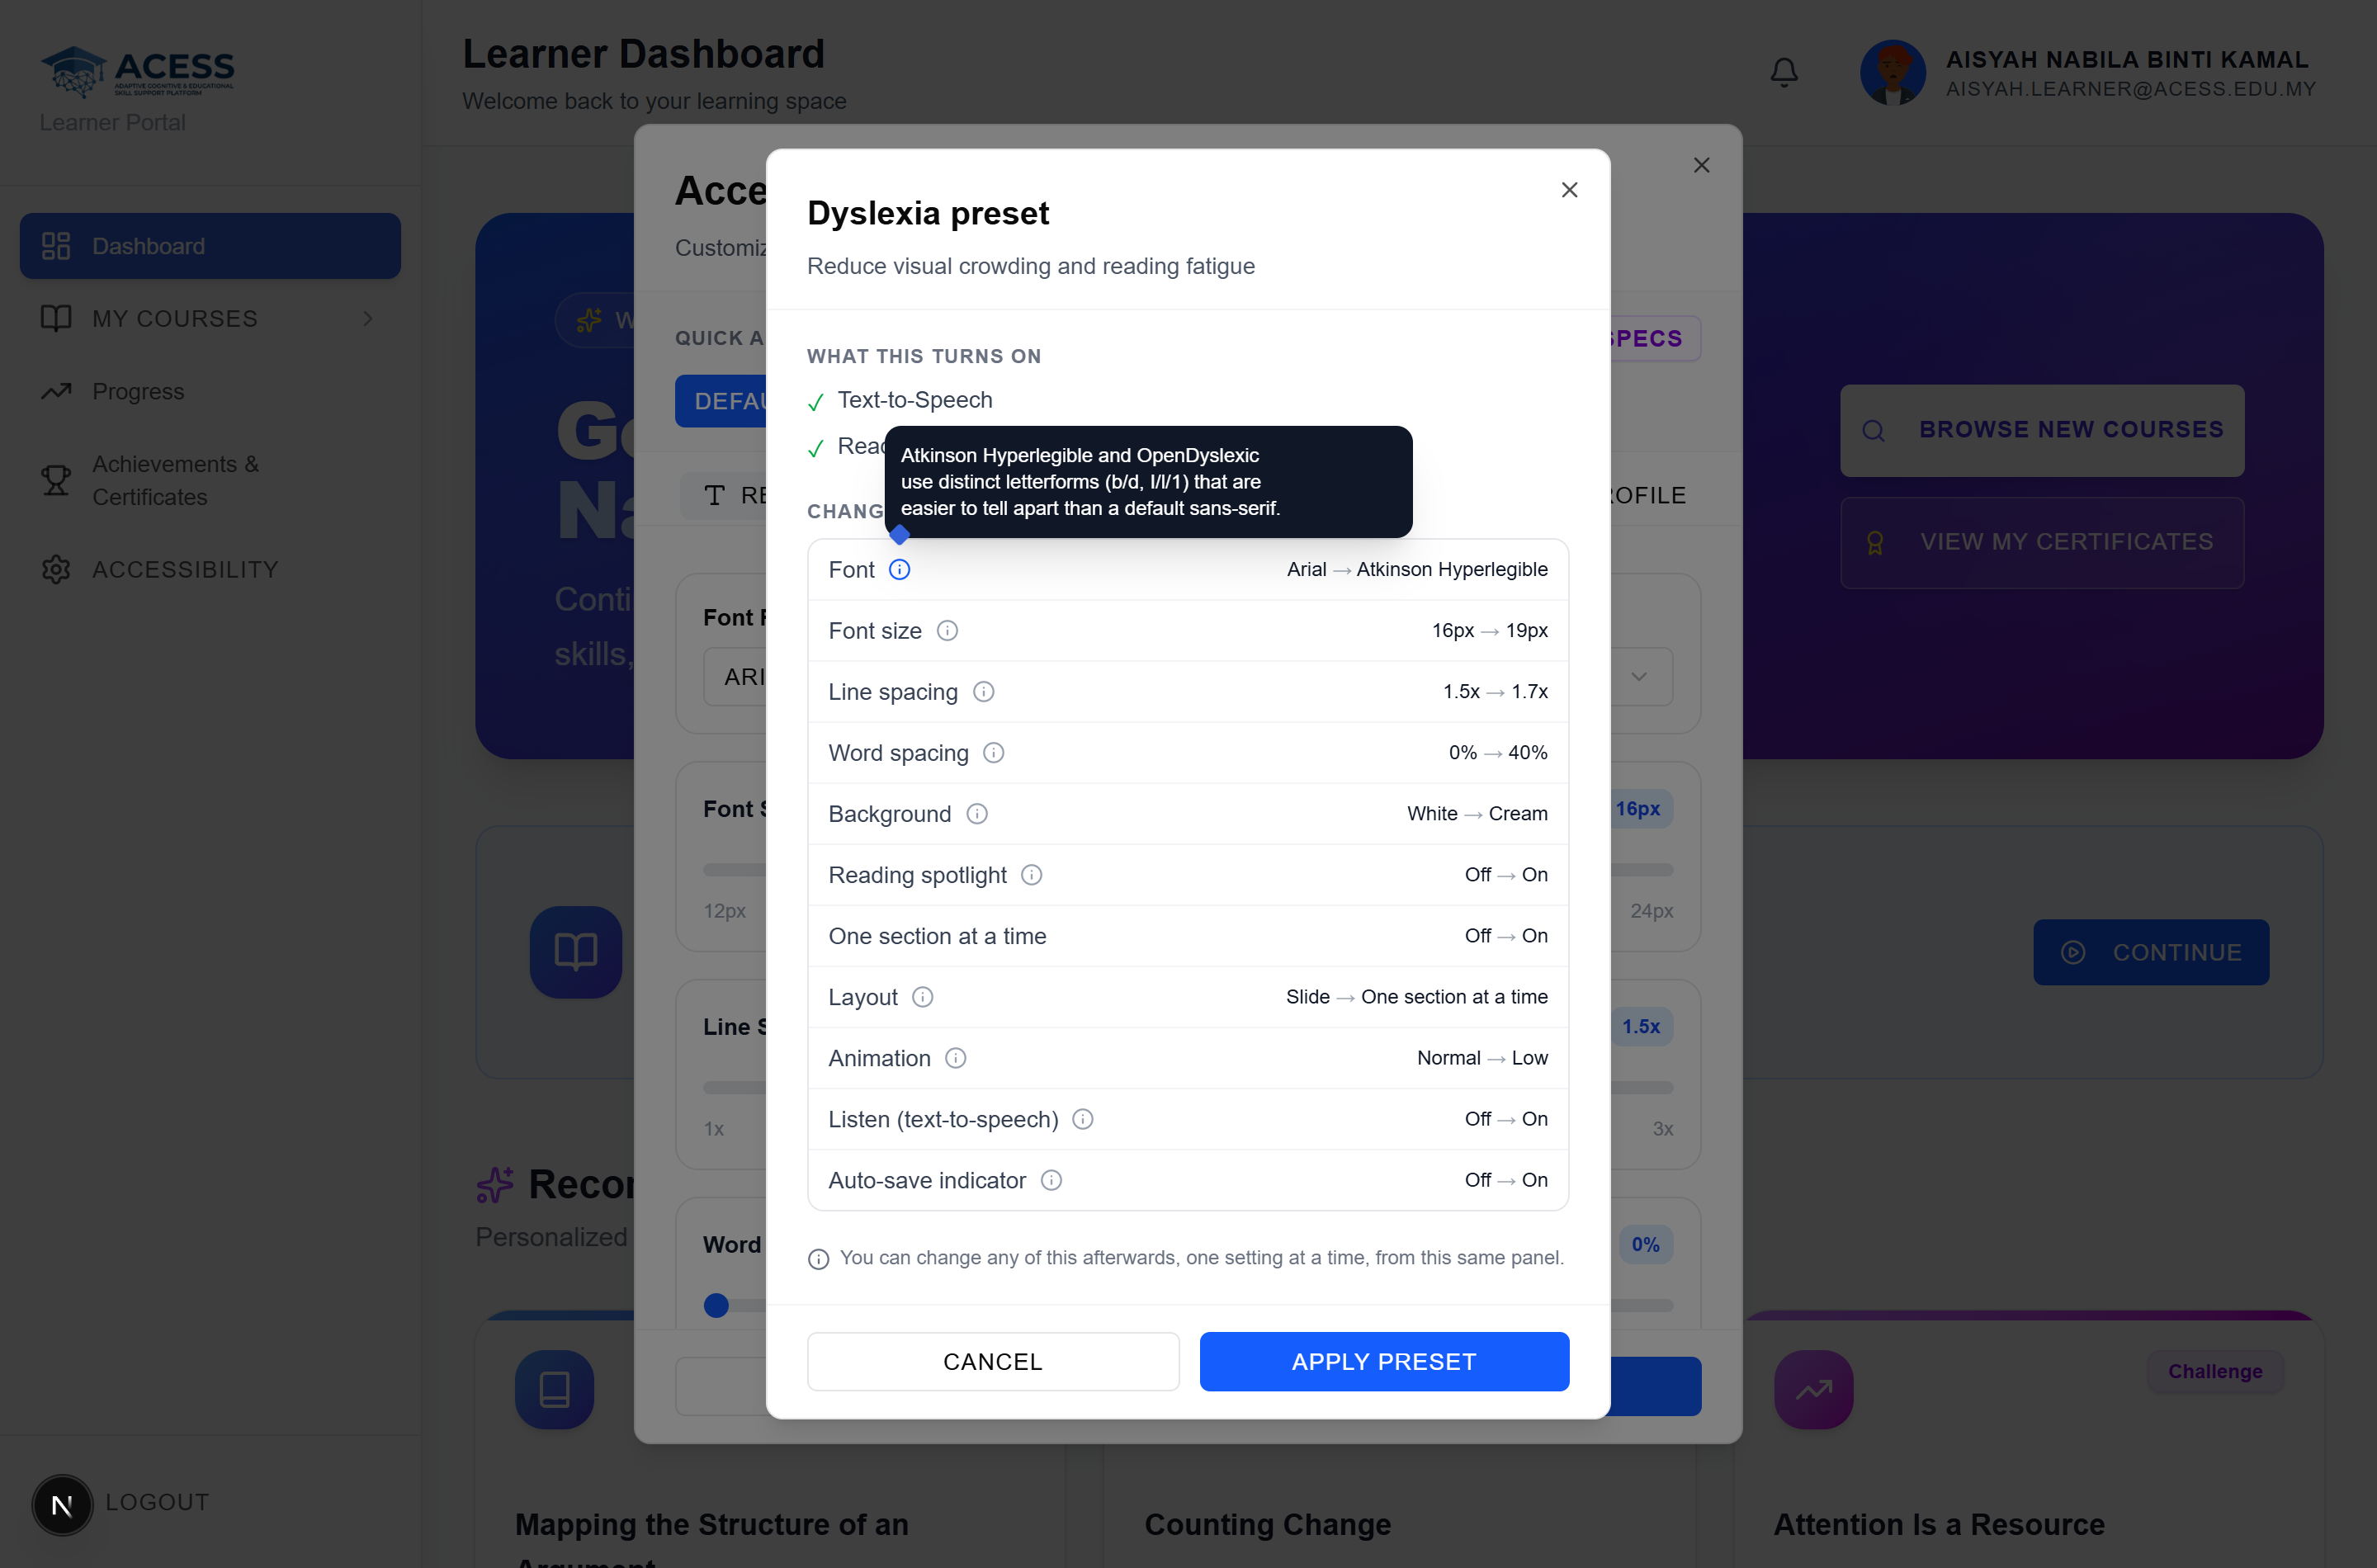
\includegraphics[width=0.86\textwidth]{Screenshots/a11y-preset-details.png}
\caption{Preset Preview Dialog}
\label{fig:preset_diff}
\end{figure}

\subsubsection{Effect of the presets on the lesson interface}

Describing an adaptive interface is less convincing than showing it. Figures~\ref{fig:preset_dyslexia} to \ref{fig:preset_autism} show the \emph{same lesson}, viewed by the \emph{same learner account}, at the same viewport size, with only the accessibility preset changed between captures. The preset values applied in each case were written by the platform's own preset function rather than set by hand, matching Table~\ref{tab:preset_effects} exactly, so the comparison shows what a learner selecting that preset actually receives.

\begin{figure}[H]
\centering
\begin{subfigure}{0.9\textwidth}
\centering
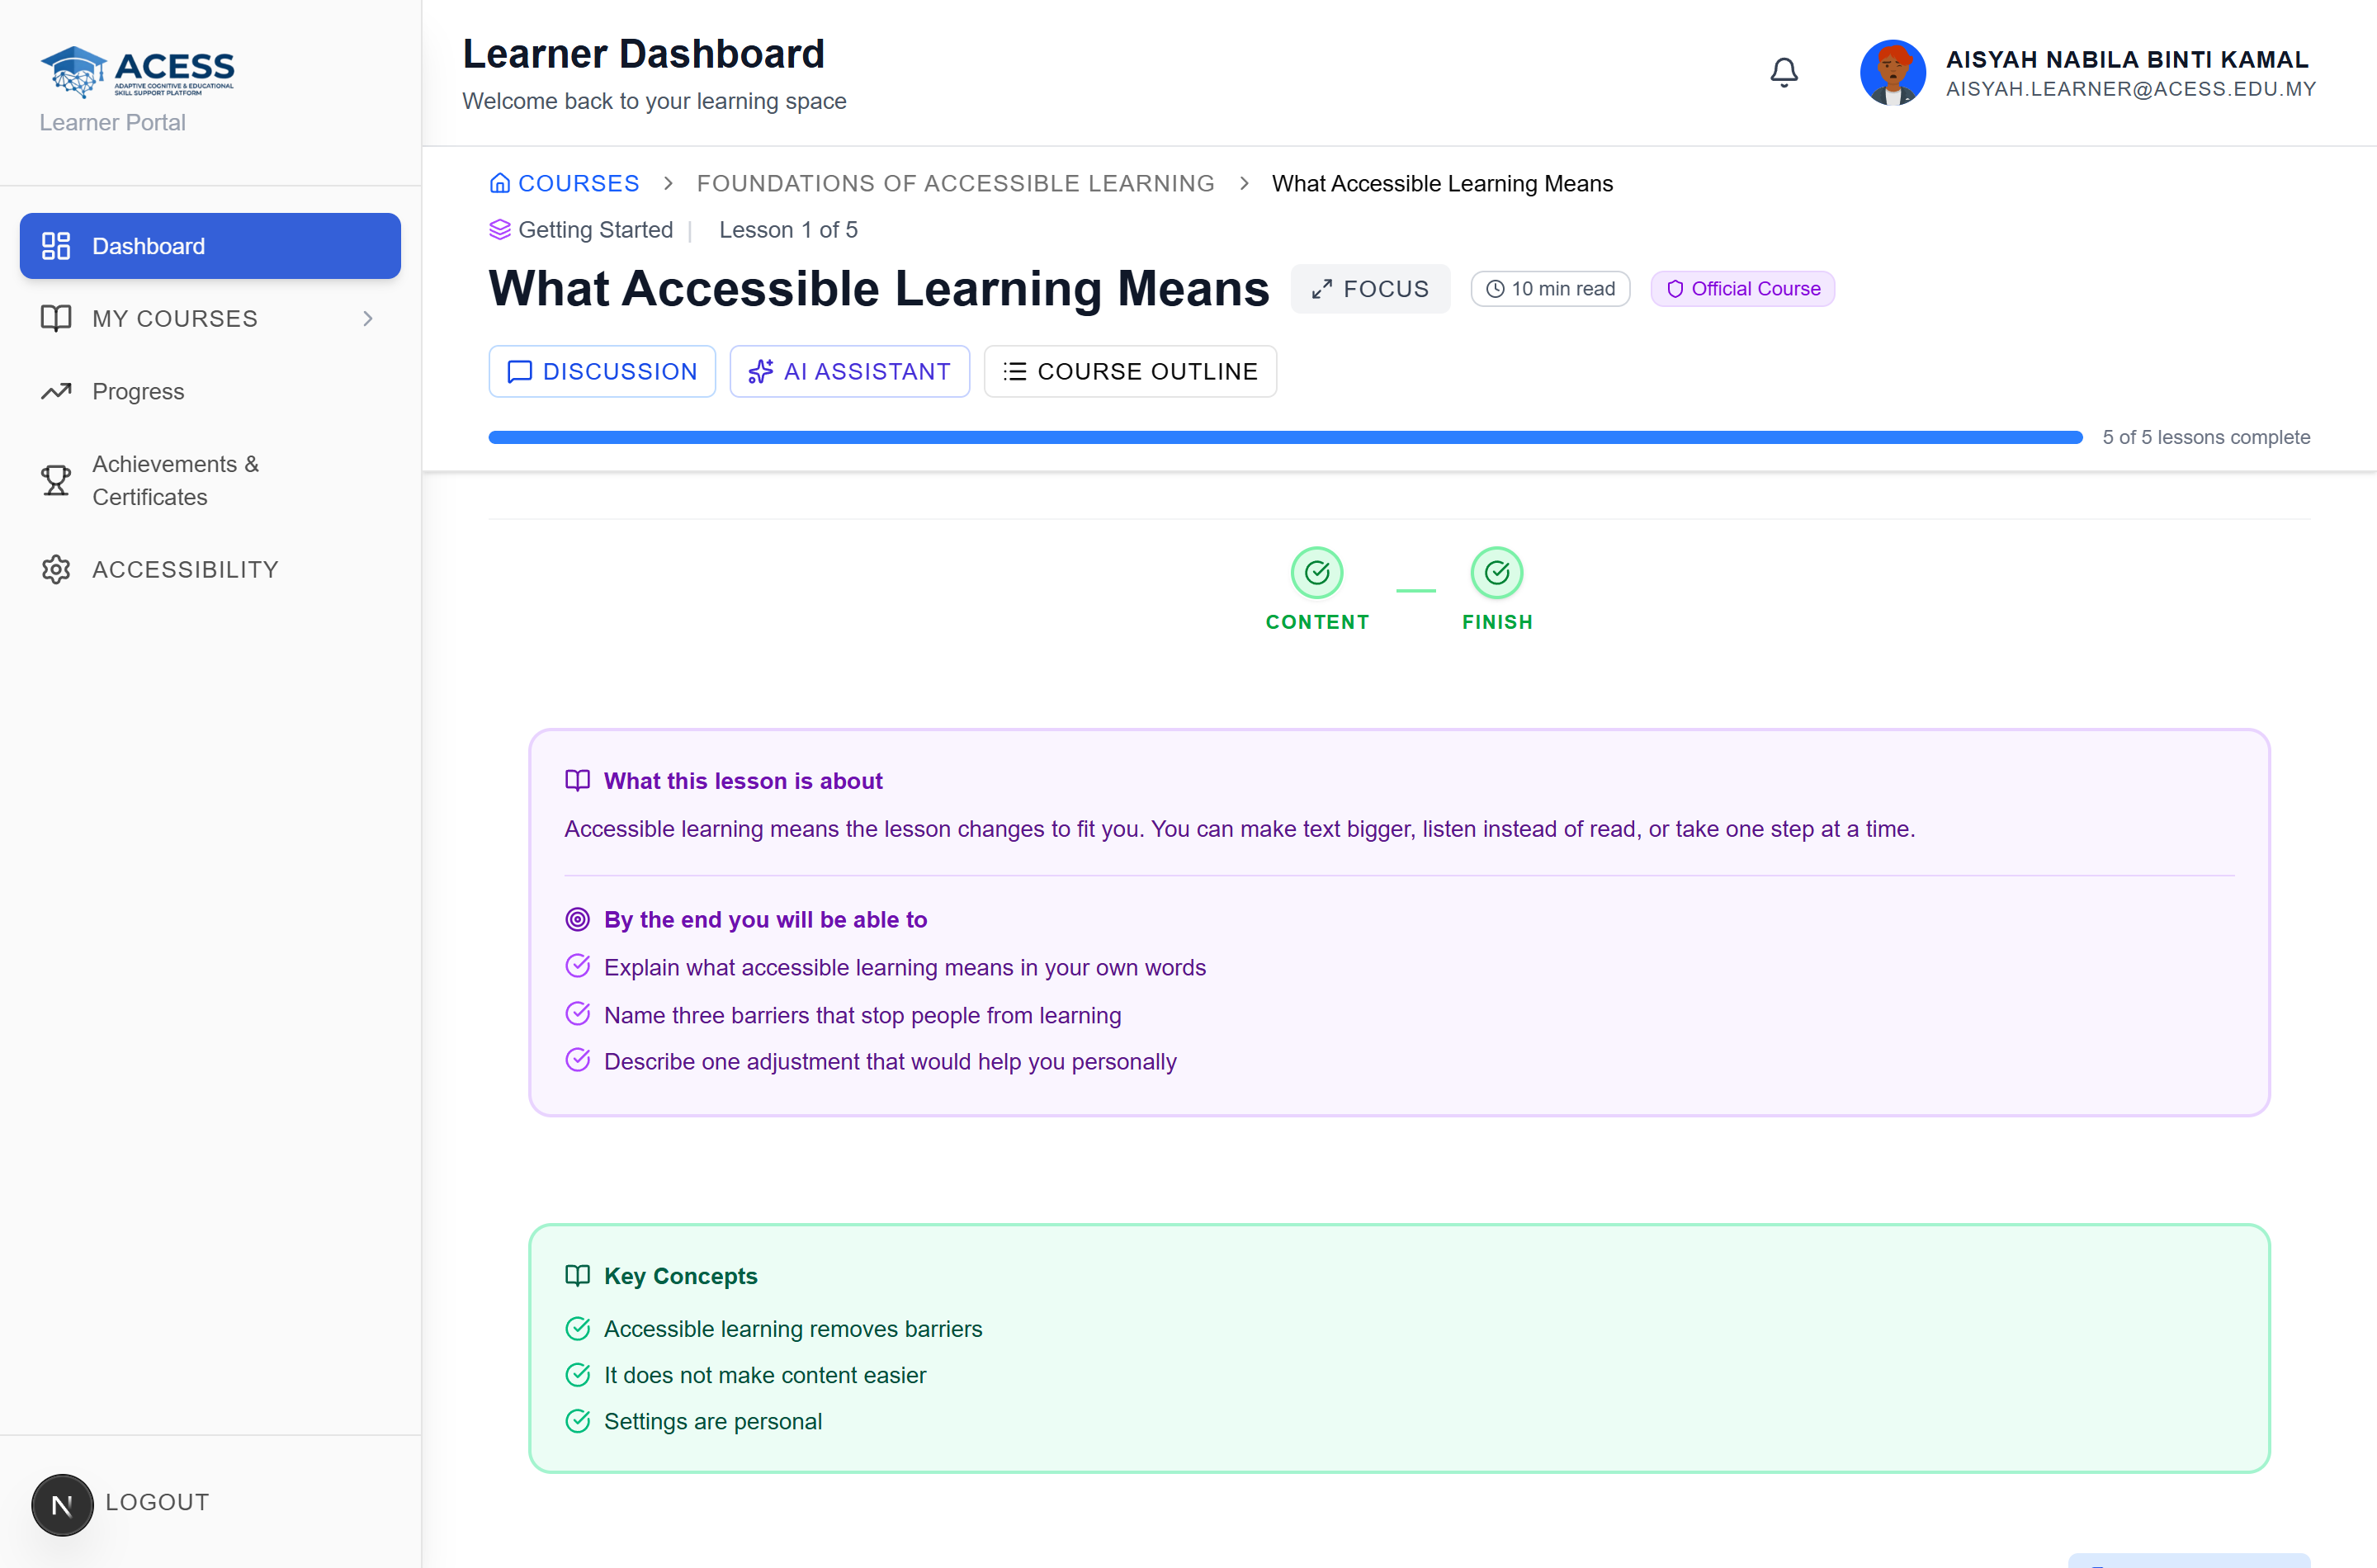
\includegraphics[width=\textwidth]{Screenshots/lesson-none.png}
\caption{Default}
\end{subfigure}

\vspace{4mm}
\begin{subfigure}{0.9\textwidth}
\centering
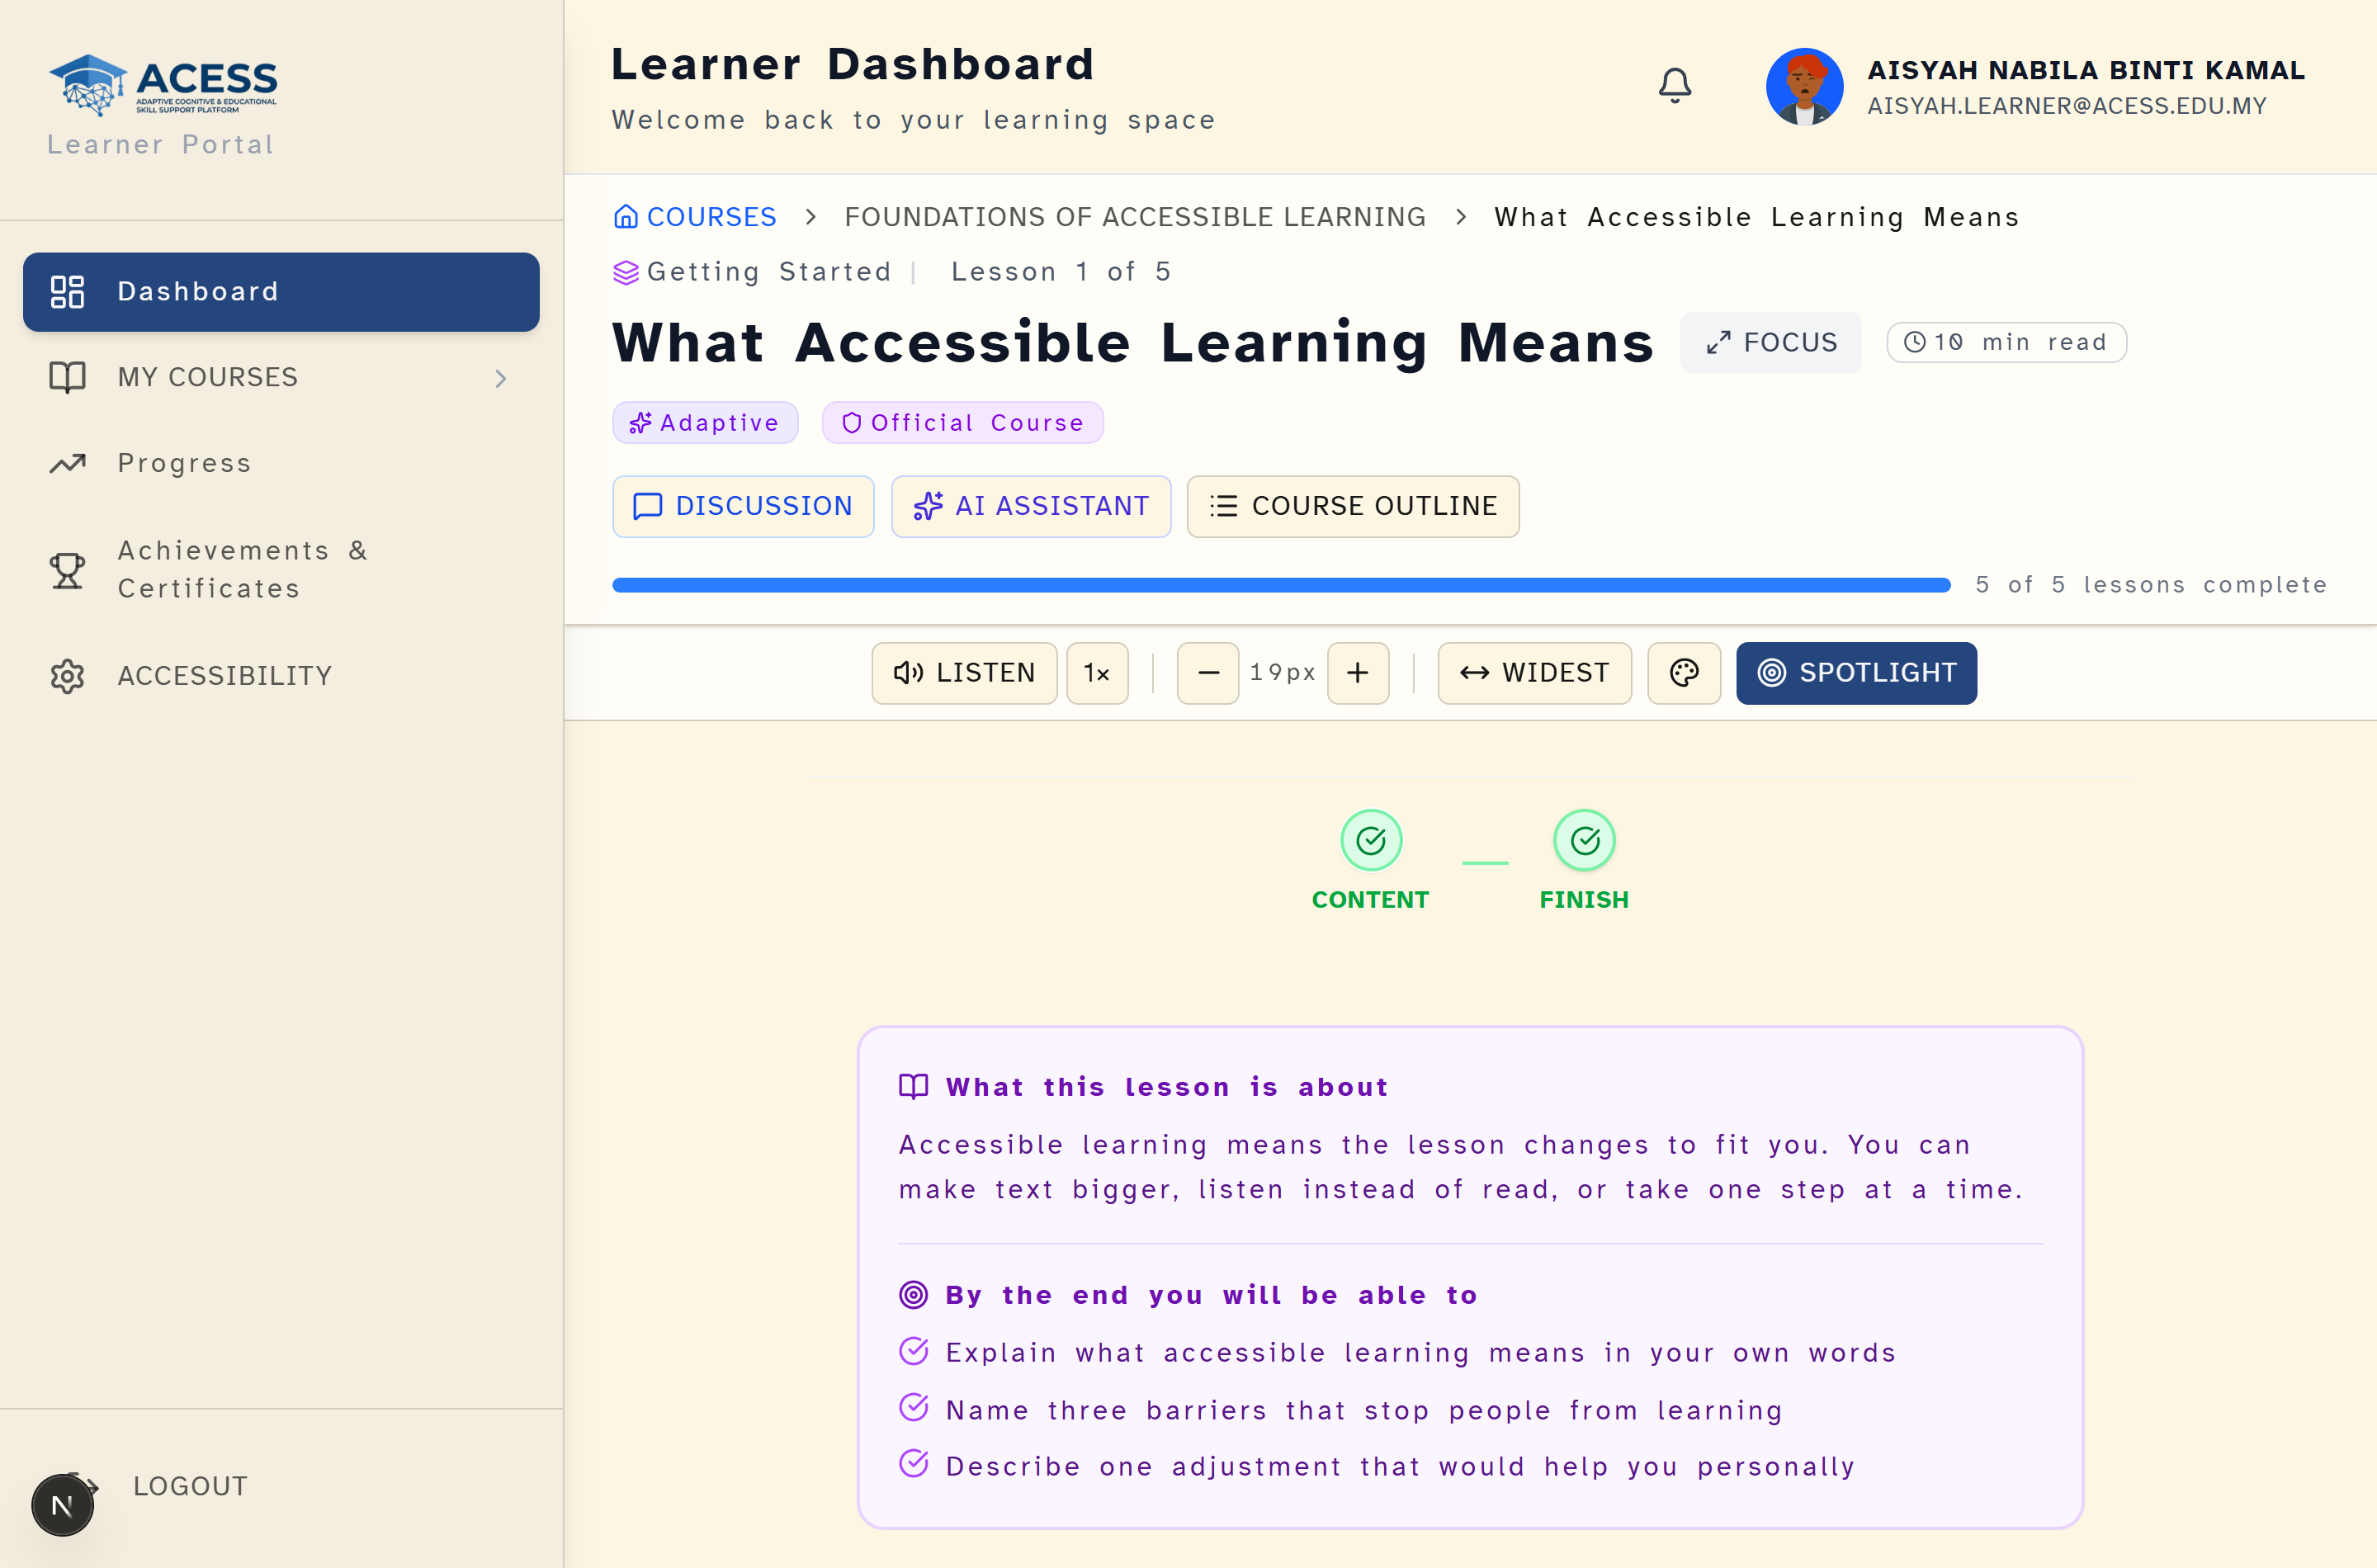
\includegraphics[width=\textwidth]{Screenshots/lesson-dyslexia.png}
\caption{Dyslexia Preset}
\end{subfigure}
\caption{Default vs.\ Dyslexia Preset}
\label{fig:preset_dyslexia}
\end{figure}

Figure~\ref{fig:preset_dyslexia} shows the change most people expect from an accessibility feature, typography and colour, but also two that are easy to miss. The reading column has narrowed rather than widened, because the constraint is expressed in characters and the characters got bigger. A persistent toolbar has also appeared below the lesson header, carrying Listen, size, spacing, tint and spotlight controls, so that the learner can adjust size, spacing, tint and read-aloud \emph{without leaving the lesson to find a settings panel}. Requiring a learner to navigate away in order to make reading easier is itself a barrier.

\begin{figure}[H]
\centering
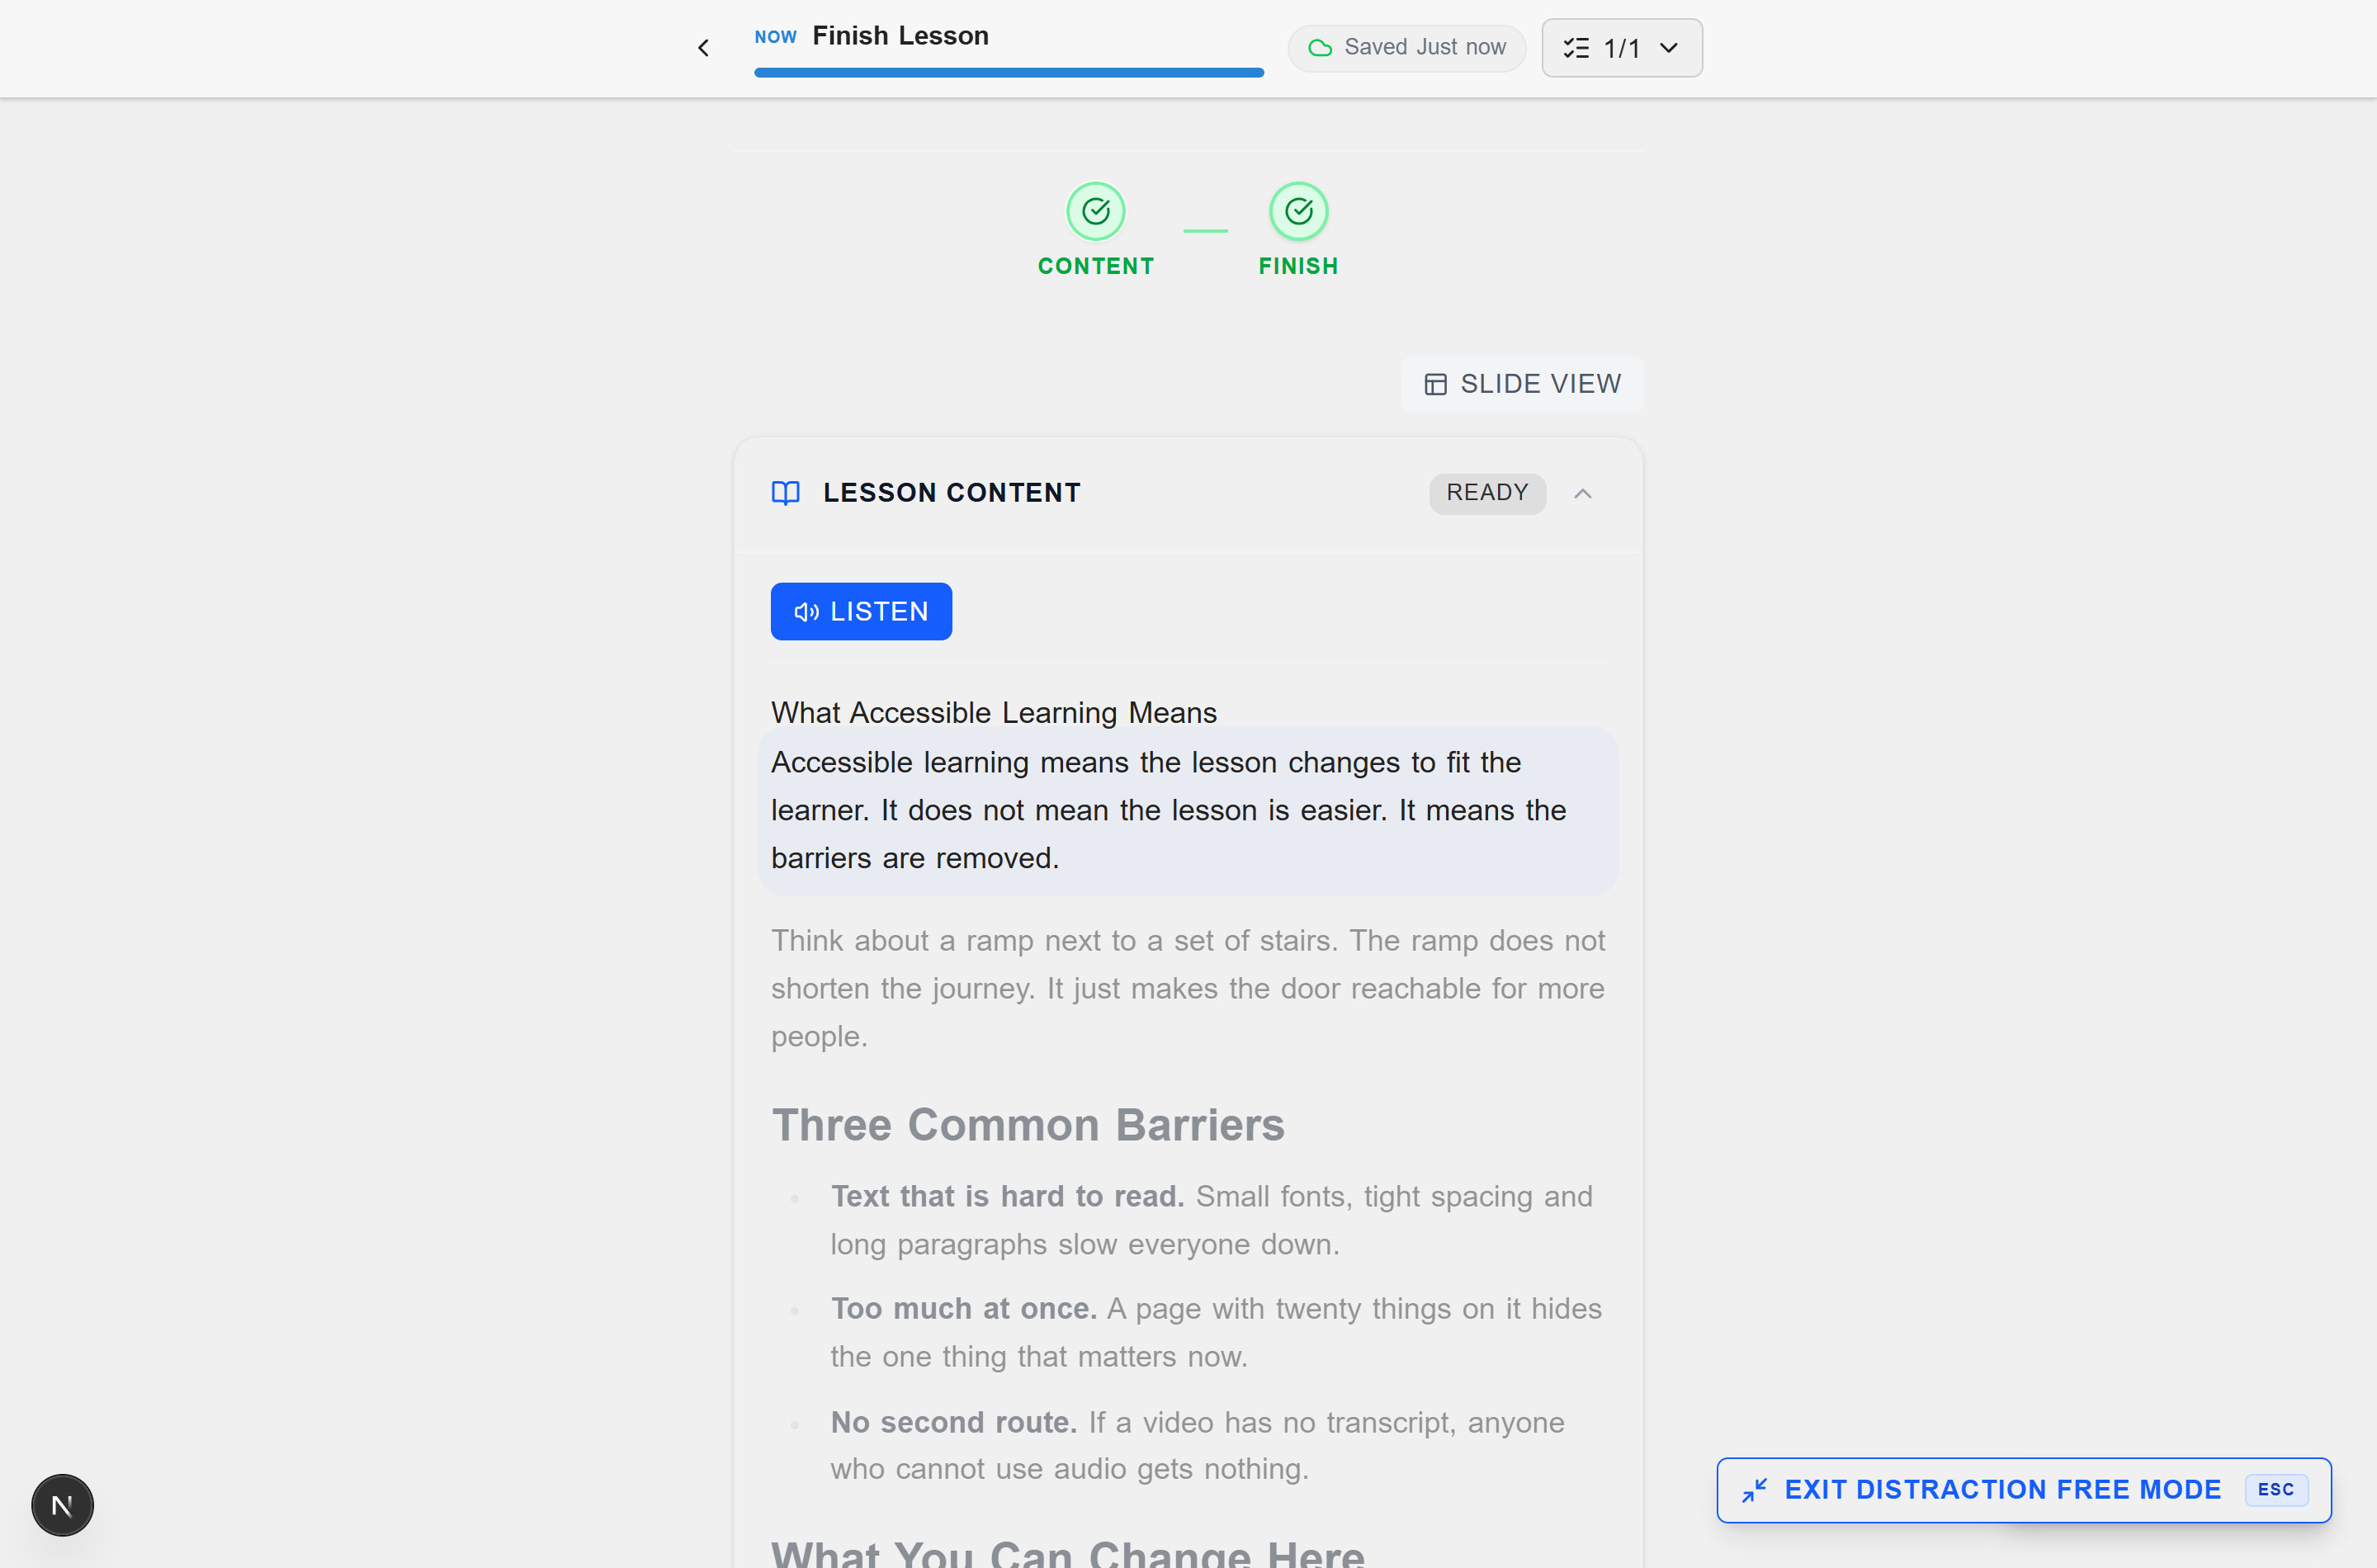
\includegraphics[width=0.92\textwidth]{Screenshots/lesson-adhd.png}
\caption{Lesson Under the ADHD Preset}
\label{fig:preset_adhd}
\end{figure}

Figure~\ref{fig:preset_adhd} is the clearest illustration of the difference between hiding things and supporting attention. The sidebar and notification chrome are removed, a persistent ``Now'' bar carries the current task together with an auto-save indicator, and the reading spotlight dims every paragraph except the one in focus. Everything that competes for attention has gone, but the reading column has \emph{not} expanded to fill the space, and it is still bounded at 66 characters. This was a defect at one point in development: distraction-free mode released the measure and produced the widest possible line length, which is the opposite of what a learner with attention difficulties needs. The exit control in the lower right, and the Escape key it advertises, exist so that the mode is never a trap.

\begin{figure}[H]
\centering
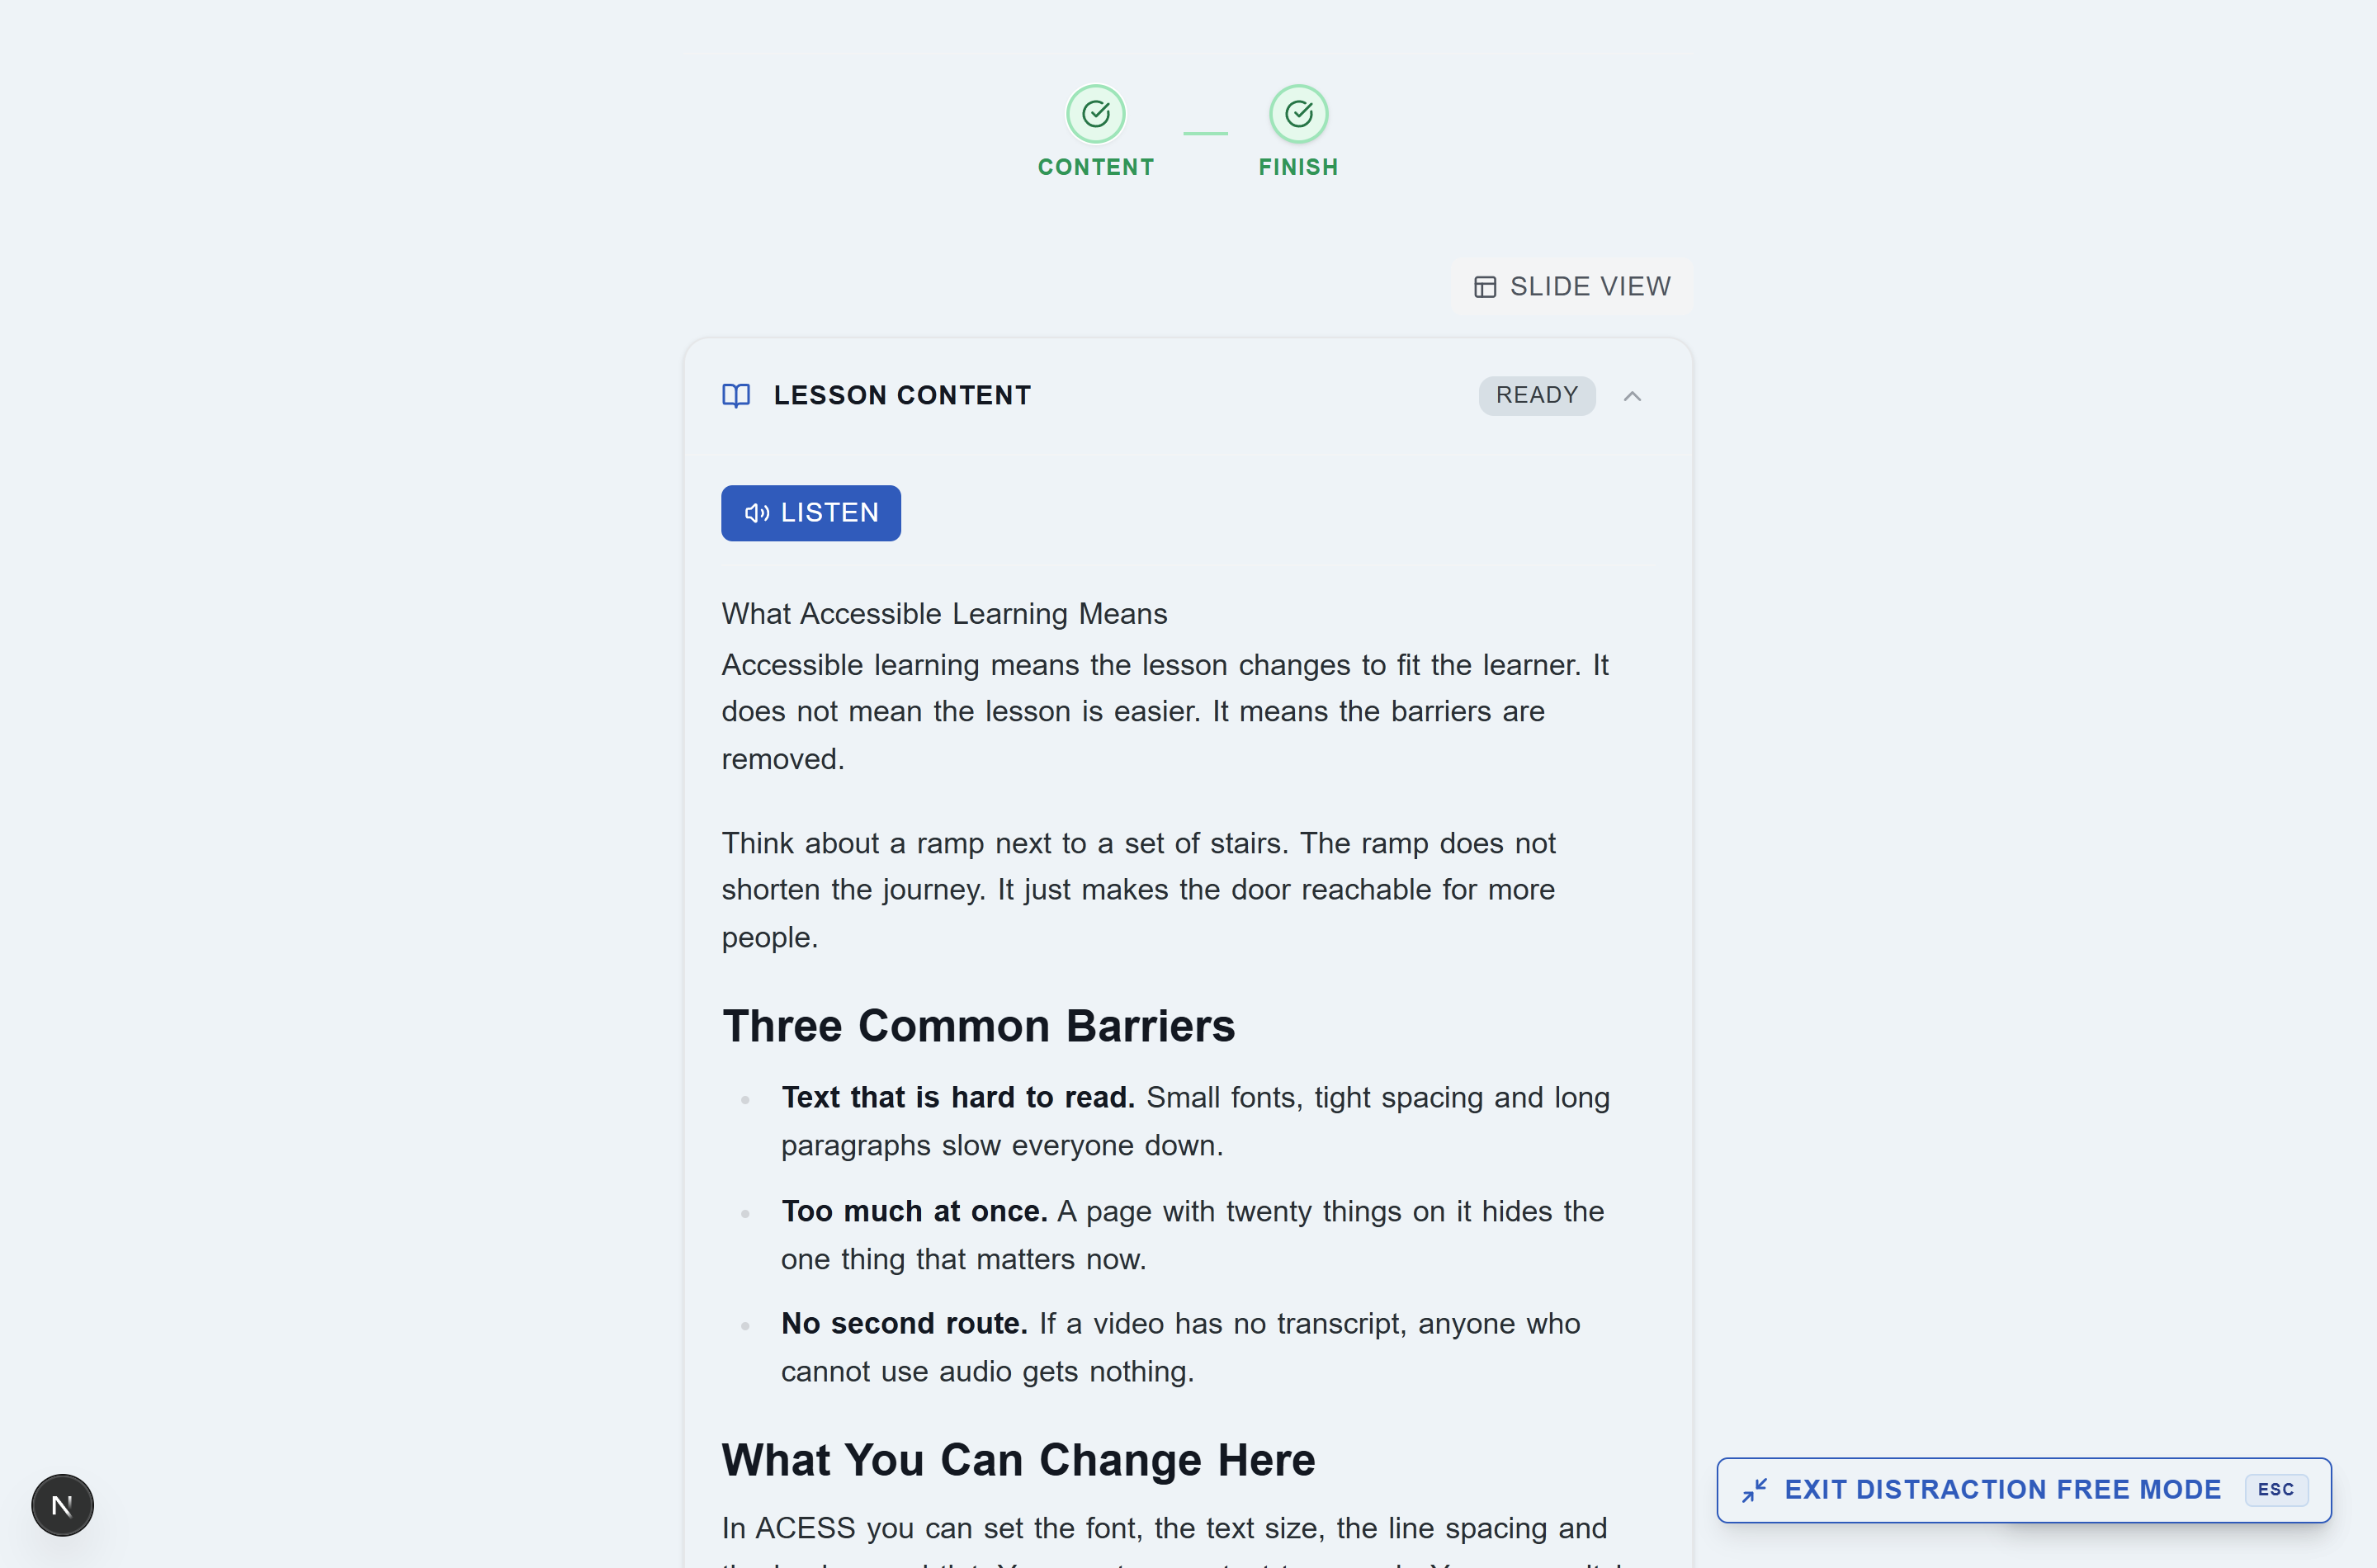
\includegraphics[width=0.92\textwidth]{Screenshots/lesson-autism.png}
\caption{Lesson Under the Autism Preset}
\label{fig:preset_autism}
\end{figure}

Figure~\ref{fig:preset_autism} shows the least visually dramatic and most structurally significant of the three, with its pale blue background, reduced colour saturation and motion removed. The palette softens, but the substantive change is the lesson's phases shown as an explicit sequence above the content, which tells the learner what this lesson consists of and how far through it they are before they begin. The reading measure is deliberately \emph{not} narrowed here: unlike dyslexia, where a narrow measure serves decoding, the Autism profile's need is predictability, and holding the same width as the default means the page does not change shape when the learner moves between a course that uses this preset and one that does not.

Figure~\ref{fig:ui_lesson_dyslexia} shows the effect at the dashboard rather than the lesson level, where the Dyslexia preset replaces the multi-column card grid with a single-column list and widens and enlarges the navigation, in place of the default card grid of Figure~\ref{fig:ui_learner_dashboard}.

\begin{figure}[H]
\centering
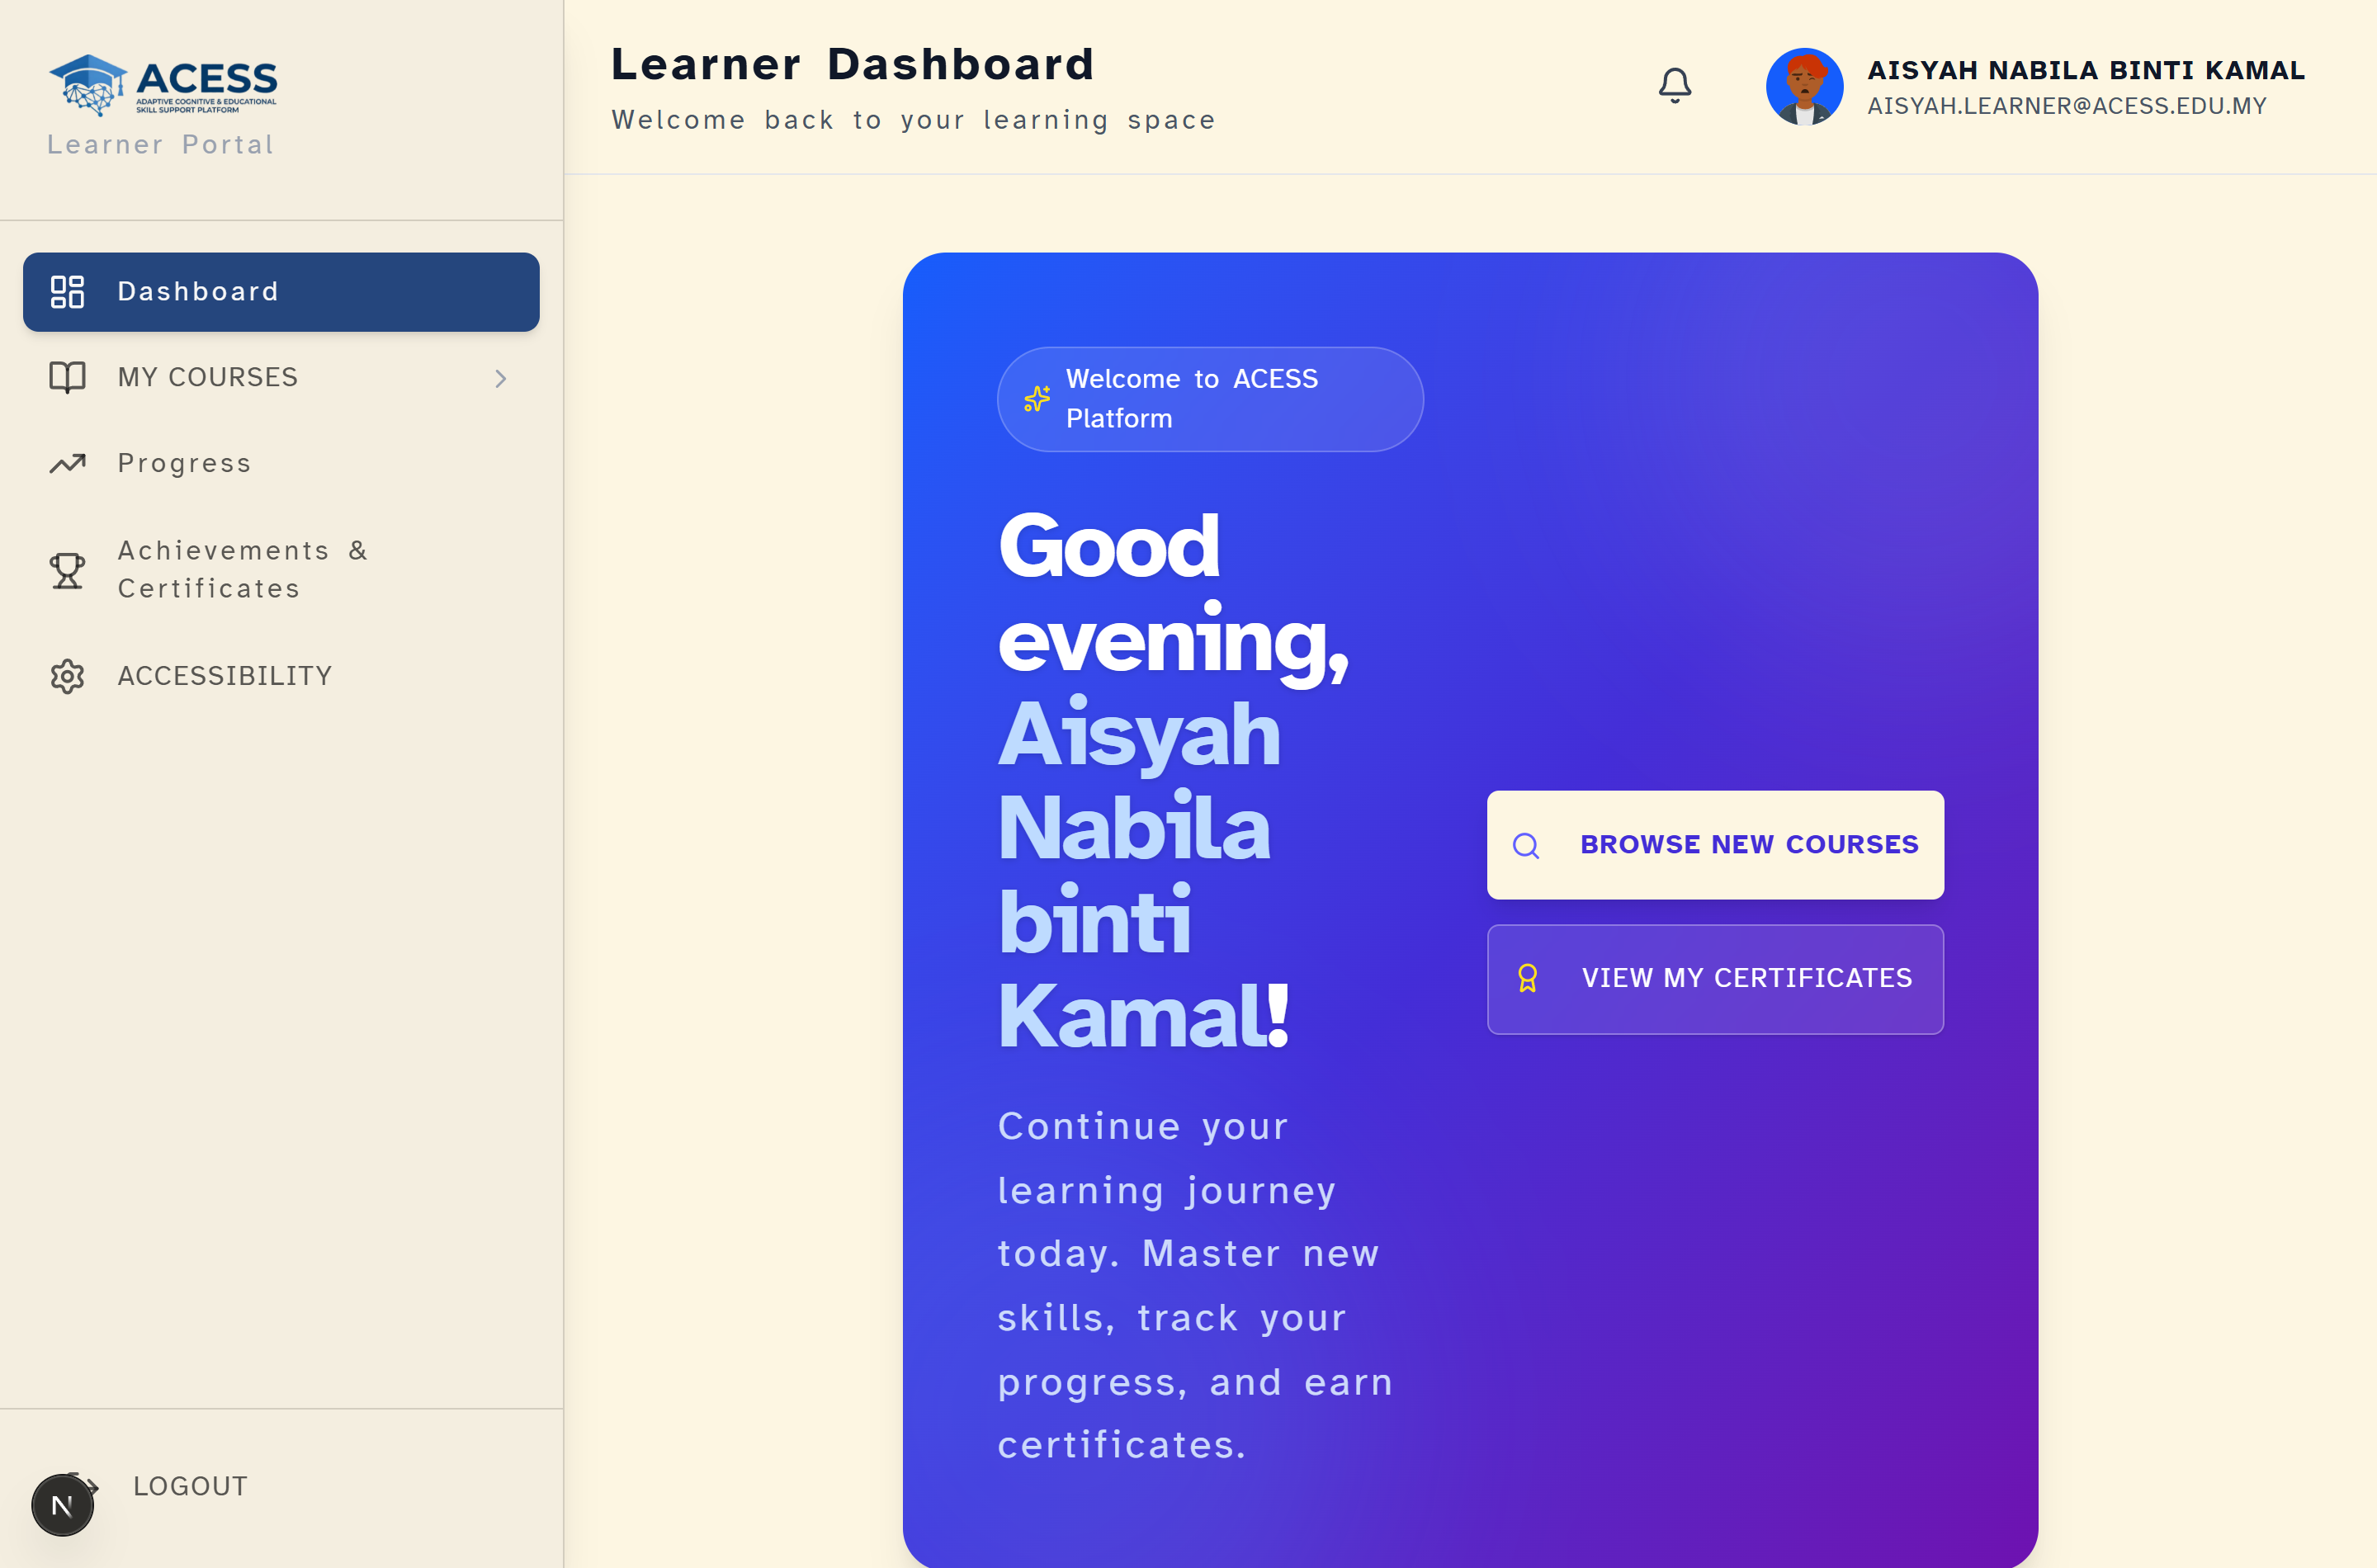
\includegraphics[width=0.92\textwidth]{Screenshots/dashboard-dyslexia.png}
\caption{Learner Dashboard Under the Dyslexia Preset}
\label{fig:ui_lesson_dyslexia}
\end{figure}

\subsubsection{Authoring-side compliance auditing}
\label{sec:a11y-audit}

The content criteria identified in Section~\ref{sec:a11y-design} cannot be met by the platform on the educator's behalf. ACESS therefore implements a deterministic auditor that evaluates a lesson while it is being written.

The engine has three properties that make its output defensible. It is \textbf{deterministic}: every rule is a fixed threshold with a published source, so the same lesson always produces the same score, since there is no model and no randomness. It is \textbf{pure and synchronous}, which is why the same engine can run against unsaved editor state on every keystroke and against rows read from the database for the course-level report, and the two necessarily agree. And it is \textbf{profile-aware}: a baseline of seven rules applies to every lesson, and a further set is added according to the course's declared focus profile (six for ADHD, five for Autism, seven for Dyslexia), so an educator writing for dyslexic readers is checked on sentence length and readability, while one writing for autistic learners is checked on figurative language and stated objectives.

Rules that cannot apply are marked \emph{not applicable} rather than failed, and are excluded from the score: a lesson with no video is not penalised for lacking a transcript. The score is the weighted proportion of applicable rules passed, banded as critical below 50, warning below 80, and good at 80 or above.

\begin{figure}[H]
\centering
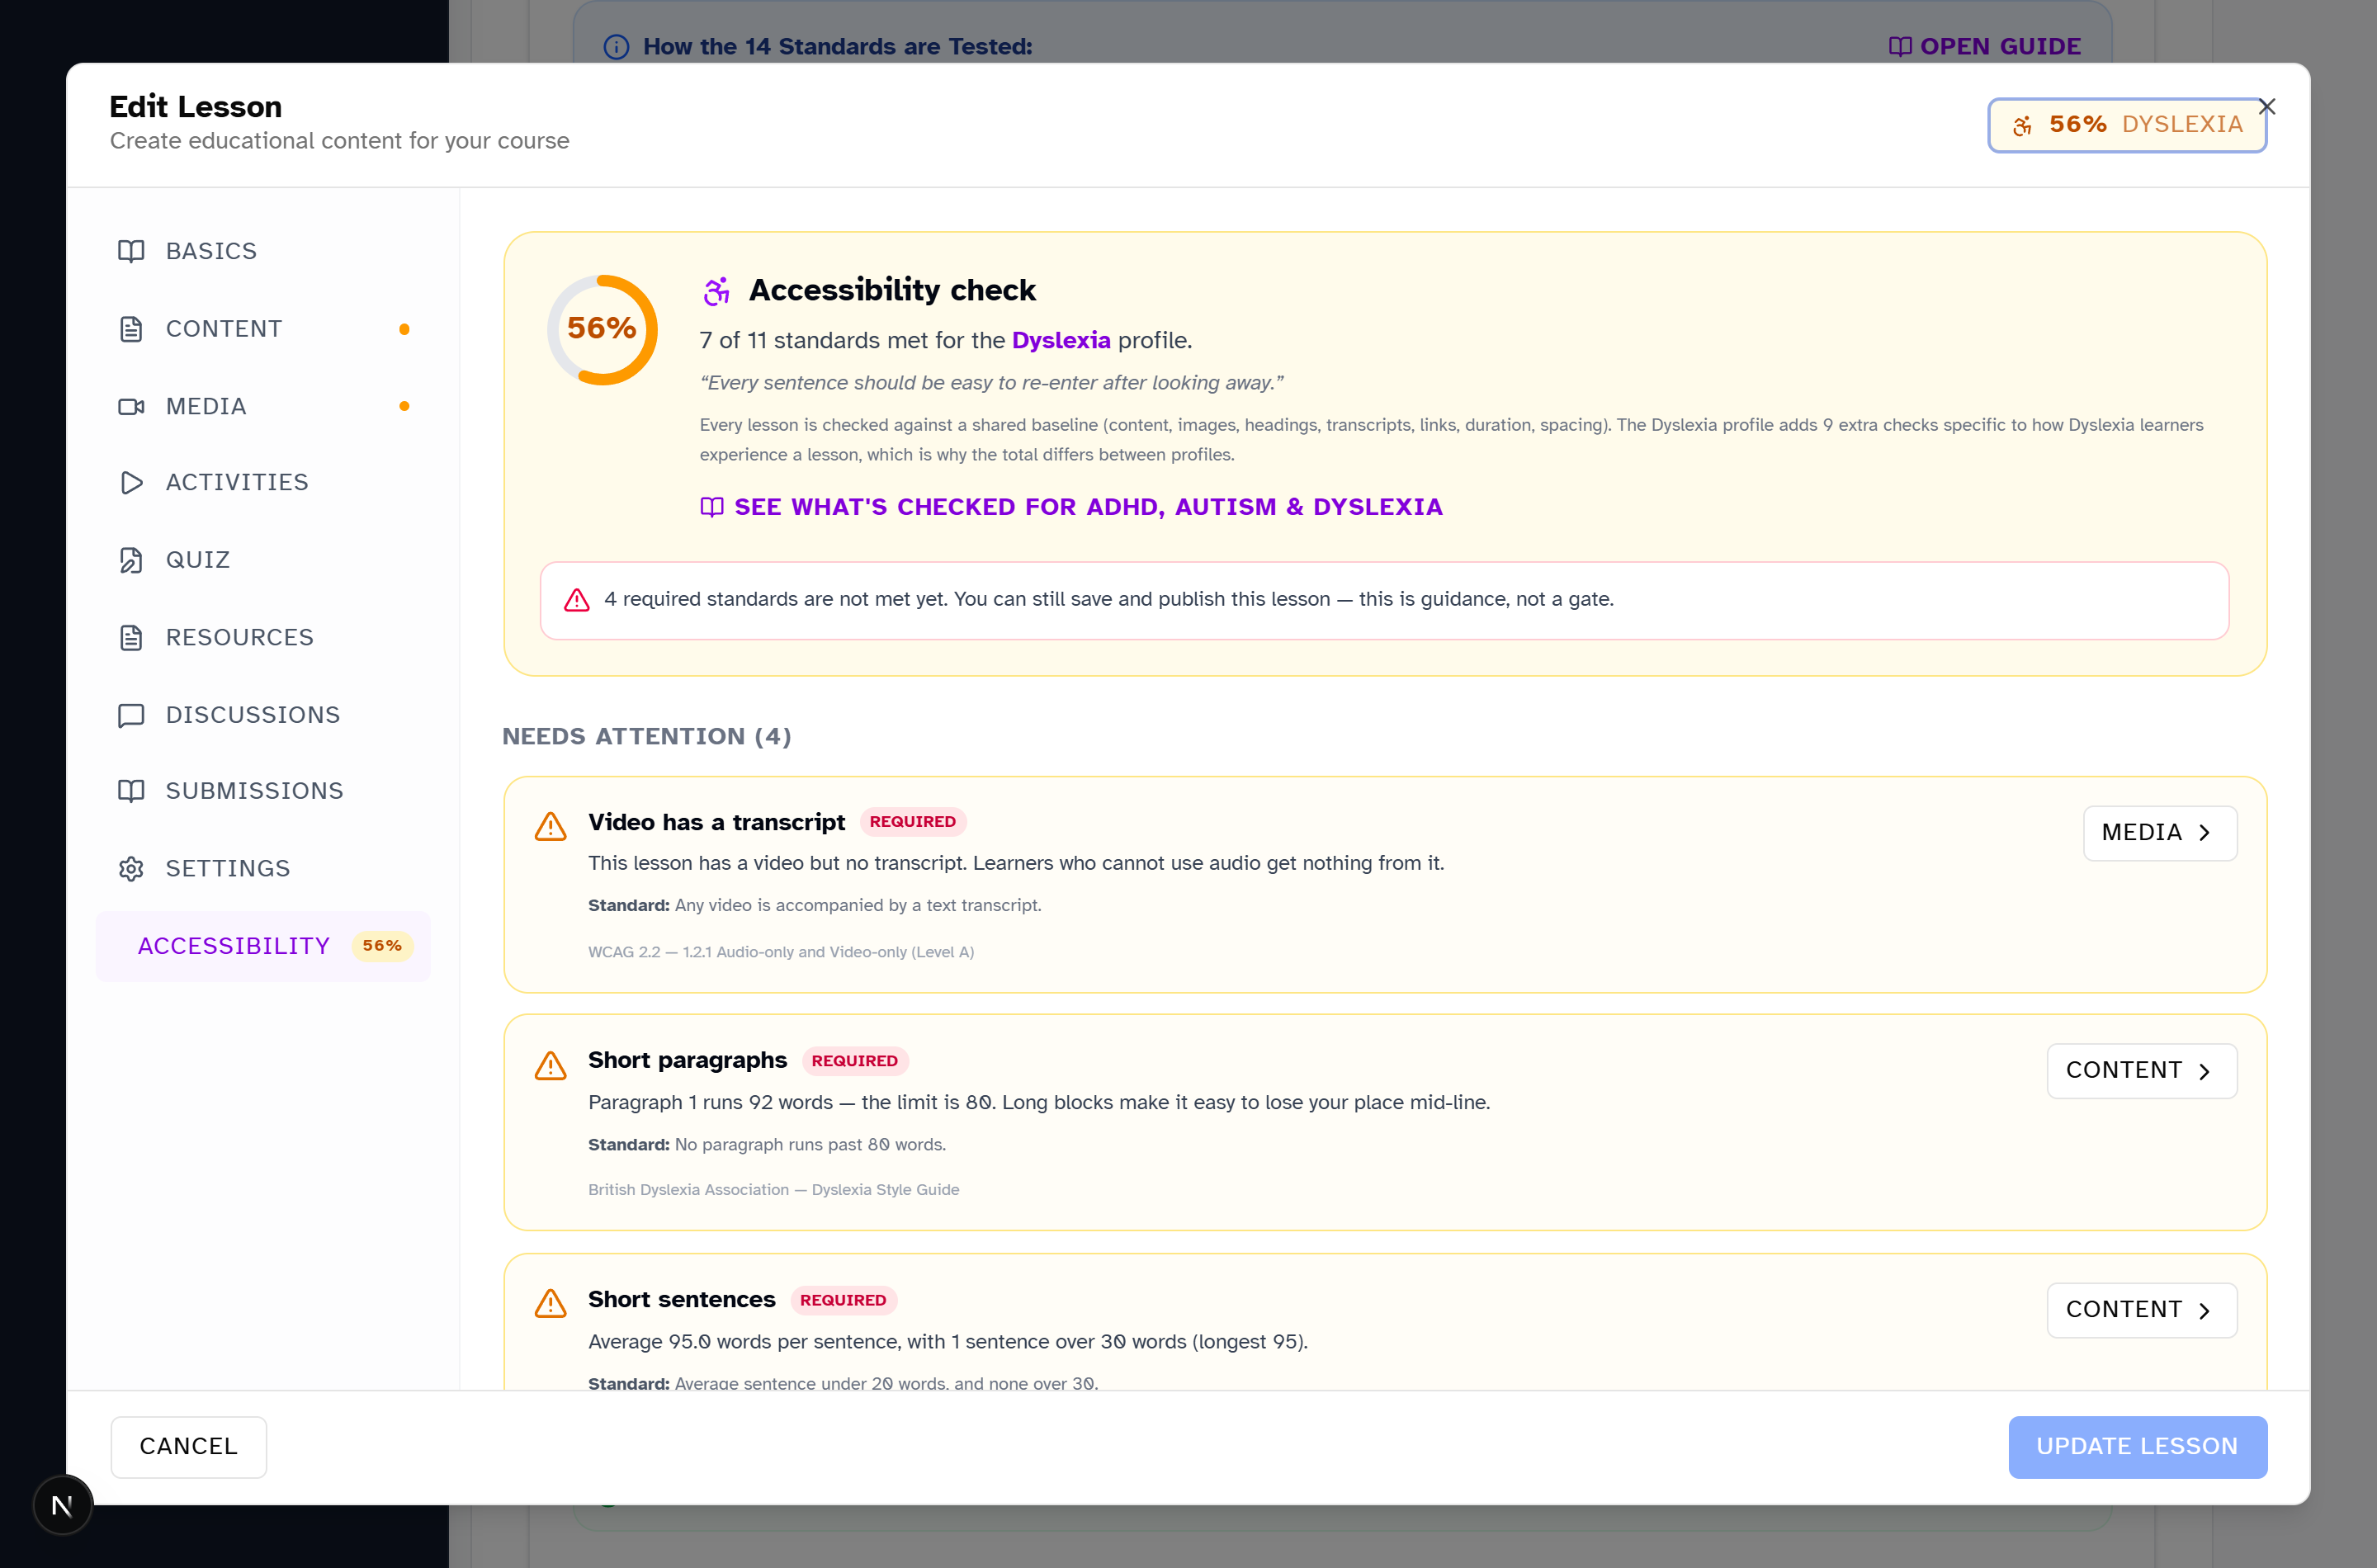
\includegraphics[width=0.94\textwidth]{Screenshots/educator-a11y-compliance.png}
\caption{Lesson Accessibility Check in the Educator Editor}
\label{fig:ui_edu_a11y}
\end{figure}

Figure~\ref{fig:ui_edu_a11y} shows the auditor reporting on a real seeded lesson, with the score for the course's declared profile shown alongside the finding list. Three further properties of that output are worth noting, because they are what distinguish it from a generic accessibility linter. Each finding states \emph{the measured value}, not merely that a rule failed: rather than ``paragraph too long'', a finding reads ``Paragraph 1 runs 92 words, and the limit is 80''. Each finding names \emph{its source}, so an educator who disagrees can consult the standard rather than the tool. And each finding carries \emph{a route to the fix}, jumping to the editor tab that owns the problem.

The panel also states, in the same view, that four required standards are unmet and that the lesson can still be saved and published. That is a deliberate policy choice. A publication gate would have produced compliance theatre (educators padding summaries to clear a word count) and would have positioned accessibility as an obstacle to teaching. The auditor advises. The educator decides. What the platform guarantees is that the decision is an informed one.

The same engine runs at course level, aggregating the fourteen standards that apply across a whole course and identifying which lessons are responsible for each unmet one, so that an educator can see whether a problem is a single weak lesson or a course-wide setting.

\subsubsection{Known accessibility gaps}
\label{sec:a11y-gaps}

This section exists because an accessibility statement with no gaps is not credible. Each of the following is a real limitation of the current build, and each is disclosed on the platform's own public accessibility statement as well as here.

\begin{enumerate}
    \item \textbf{No assistive technology has been tested against this build.} No screen reader (NVDA, VoiceOver or TalkBack) and no other assistive technology has been used against ACESS. Every claim in Table~\ref{tab:wcag_map} is verified by reading and tracing the code that implements it and by exercising it in a browser, not by using it as a screen-reader user would. This is the most significant limitation in this chapter.
    \item \textbf{No disabled learner has tested the platform.} No learner with lived experience of dyslexia, ADHD or autism took part in building or evaluating it. The design draws on published guidance rather than on the people it is for, which is a real methodological weakness and is discussed further in Section~\ref{sec:design-limitations}.
    \item \textbf{The ``Muted Colors'' setting is over-broad.} It is implemented as a global saturation filter, so it desaturates error, warning and success colours along with everything else, making status information harder to distinguish, which is the opposite of the intent. A correct fix requires reworking colour tokens throughout the stylesheet and was judged too large to attempt without visual verification. The setting's own description in the platform catalogue states this current behaviour rather than the intended one.
    \item \textbf{The ``Keyboard navigation'' setting does not do what its label promises.} It sets a document attribute that nothing currently reads. Keyboard operability should not be optional in any case. The entry is retained in the catalogue so that the gap is visible rather than silently absent, pending either implementation or redefinition.
    \item \textbf{Only one preset can be active at a time.} A learner who would benefit from Dyslexia typography together with ADHD pacing supports must currently choose one and adjust the rest manually. Composable profiles are the most frequently identified extension to this design.
    \item \textbf{One drag-and-drop mode has no non-drag alternative.} The ``categories'' mode and every other activity type have a keyboard path and, where relevant, a non-drag alternative. The ``diagram'' mode, which places labels at arbitrary coordinates on an image, does not.
    \item \textbf{Read-from-here is pointer-only.} Clicking a paragraph during read-aloud restarts speech from that paragraph, but this is not reachable from the keyboard. The Listen control remains the keyboard baseline.
    \item \textbf{No quantitative accessibility baseline was captured.} No before-and-after measurement of learner outcomes exists, because no baseline was taken before the accessibility work began. The comparisons in this chapter are therefore demonstrations that the interface adapts as designed, not evidence that the adaptation improves learning outcomes. Establishing that would require the study described in Section~\ref{sec:design-limitations}.
\end{enumerate}

\subsection{Data Dictionary and Normalisation}
\label{sec:data-dict}

\subsubsection{Normalisation}

The schema is normalised to Third Normal Form, with two documented and deliberate departures. The reasoning is set out here rather than left implicit, because both departures would otherwise read as oversights.

Every table has a single-column surrogate primary key, so first normal form holds trivially and no partial dependency on part of a composite key is possible, which gives second normal form. Third normal form (no transitive dependency of a non-key attribute on another non-key attribute) holds throughout the operational tables: a lesson stores its \tcode{course_id} but not its course's title, a quiz attempt stores its \tcode{enrollment_id} but not the learner's name, and progress rows carry no copy of the lesson's duration.

The two departures are:

\begin{enumerate}
    \item \textbf{The certificate record is deliberately denormalised.} \tcode{certificates} stores \tcode{learner_name}, \tcode{course_title}, \tcode{educator_name}, \tcode{institution_name} and \tcode{course_duration_hours} as literal values, even though every one of them could be joined for. This is intentional and is the correct design for this entity: a certificate is a statement about a moment in time. If the course were later renamed, or the learner changed their display name, a joined certificate would silently rewrite history and no longer match the PDF the learner already holds. Freezing the values at issue is what makes the document verifiable years later.
    \item \textbf{Accessibility and notification preferences are stored as JSON documents} on \tcode{user_profiles} rather than decomposed into columns. Strictly, this is a repeating group and is not first normal form. It was chosen because the setting vocabulary changes considerably faster than the rest of the schema (the platform's own catalogue currently defines twenty-four learner-facing settings, and that list has been revised repeatedly during development), and because every consumer reads the entire object at once rather than querying individual settings. The cost is that the database cannot constrain an individual setting's value. The platform compensates by defining the permitted vocabulary in a single application-level catalogue against which an automated check runs, so that a setting cannot exist in the data without also existing in that catalogue.
\end{enumerate}

Two further points are worth recording. First, the schema contains no many-to-many relationship implemented without a junction table: \tcode{user_achievements} and \tcode{course_favorites} both exist precisely to resolve one. Second, one denormalised column pair was removed during the schema consolidation described in Section~\ref{sec:phys-db}: \tcode{lessons.chapter_title} duplicated \tcode{course_chapters.title} and could disagree with it, so the current schema is closer to 3NF than the design documented in the previous revision of this report.

\subsubsection*{Reading the tables}

The following tables constitute the physical schema of the ACESS PostgreSQL database as it currently stands: 36 base tables and 364 columns (370 including the six columns of the \tcode{quiz_options_scoped} view, which is described in Section~\ref{sec:phys-db}). They were generated directly from the live database catalogue rather than transcribed, so the attribute names, types, defaults and constraints in them are the ones the database actually holds. The \textbf{Constraint} column reports the key role, referential target, uniqueness and nullability of each attribute. \texttt{CHECK} constraints, which apply to a value rather than to a column's structure, are discussed with the physical design in Section~\ref{sec:phys-db}.

\subsubsection{Core Identity and Configuration}

Tables~\ref{tab:dd_users} to~\ref{tab:dd_adaptive_interactions} define the 8 entities of the core identity and configuration domain.

\textbf{1. Table: users}

\begin{table}[H]
\caption{Users Data Dictionary}
\label{tab:dd_users}
\vspace{-4mm}
\begin{center}
\renewcommand{\arraystretch}{1.15}
\scriptsize
\begin{tabular}{|>{\raggedright\arraybackslash\tabbreak}p{2.67cm}|>{\raggedright\arraybackslash\tabbreak}p{2.93cm}|>{\raggedright\arraybackslash\tabbreak}p{2.67cm}|>{\raggedright\arraybackslash\tabbreak}p{4.51cm}|}
\hline
\textbf{Attribute} & \textbf{Type} & \textbf{Constraint} & \textbf{Description} \\ \hline
id & uuid & PRIMARY KEY & Unique identifier (UUID v4). \\ \hline
email & character varying & UNIQUE, NOT NULL & User email address, used for login and notifications. \\ \hline
role & character varying & NOT NULL & User role: learner, educator, or admin. \\ \hline
is\_active & boolean DEFAULT true & NOT NULL & Soft-ban flag, inactive users cannot log in. \\ \hline
email\_verified\_at & timestamp & - & Timestamp when user confirmed email via verification link, NULL if unverified. \\ \hline
last\_login\_at & timestamp & - & Timestamp of last successful login. \\ \hline
created\_at & timestamp DEFAULT now() & NOT NULL & Timestamp when the record was created. \\ \hline
updated\_at & timestamp DEFAULT now() & NOT NULL & Timestamp of the last modification. \\ \hline
deleted\_at & timestamp & - & Soft-delete timestamp, null if not deleted. \\ \hline
full\_name & text & - & User's display name shown across the platform. \\ \hline
instructor\_application\_status & text & - & Status of educator application. \\ \hline
\end{tabular}
\end{center}
\end{table}

\textbf{2. Table: user\_profiles}

\begin{table}[H]
\caption{User Profiles Data Dictionary}
\label{tab:dd_user_profiles}
\vspace{-4mm}
\begin{center}
\renewcommand{\arraystretch}{1.15}
\scriptsize
\begin{tabular}{|>{\raggedright\arraybackslash\tabbreak}p{2.67cm}|>{\raggedright\arraybackslash\tabbreak}p{2.93cm}|>{\raggedright\arraybackslash\tabbreak}p{2.67cm}|>{\raggedright\arraybackslash\tabbreak}p{4.51cm}|}
\hline
\textbf{Attribute} & \textbf{Type} & \textbf{Constraint} & \textbf{Description} \\ \hline
id & uuid DEFAULT gen\_random\_uuid() & PRIMARY KEY & Unique identifier (UUID v4). \\ \hline
user\_id & uuid & FK $\rightarrow$ users, UNIQUE, NOT NULL & Foreign key referencing users.id. \\ \hline
username & text & UNIQUE & Public-facing username handle. \\ \hline
avatar\_url & text & - & URL to the user's profile image. \\ \hline
phone\_number & text & - & Contact phone number for account recovery and notifications. \\ \hline
birth\_date & date & - & User's date of birth for age verification and age-group analytics. \\ \hline
bio & text & - & Short biographical text for educator profiles. \\ \hline
country & text & - & ISO 3166-1 country code for regional content localisation. \\ \hline
preferred\_language & text DEFAULT 'en' & - & UI language code (en, ms). \\ \hline
created\_at & timestamptz DEFAULT now() & - & Timestamp when the record was created. \\ \hline
updated\_at & timestamptz DEFAULT now() & - & Timestamp of the last modification. \\ \hline
disability\_type & character varying & - & Disability classification for adaptive engine. \\ \hline
accessibility\_prefs & jsonb DEFAULT '{}' & - & JSON object storing active accessibility settings (font size, colour scheme, TTS rate, dyslexia font toggle). \\ \hline
notification\_prefs & jsonb DEFAULT '{}' & - & JSON object storing notification delivery preferences (email, in-app, frequency). \\ \hline
\end{tabular}
\end{center}
\end{table}

\textbf{3. Table: referral\_codes}

\begin{table}[H]
\caption{Referral Codes Data Dictionary}
\label{tab:dd_referral_codes}
\vspace{-4mm}
\begin{center}
\renewcommand{\arraystretch}{1.15}
\scriptsize
\begin{tabular}{|>{\raggedright\arraybackslash\tabbreak}p{2.67cm}|>{\raggedright\arraybackslash\tabbreak}p{2.93cm}|>{\raggedright\arraybackslash\tabbreak}p{2.67cm}|>{\raggedright\arraybackslash\tabbreak}p{4.51cm}|}
\hline
\textbf{Attribute} & \textbf{Type} & \textbf{Constraint} & \textbf{Description} \\ \hline
id & uuid DEFAULT gen\_random\_uuid() & PRIMARY KEY & Unique identifier (UUID v4). \\ \hline
code & text & UNIQUE, NOT NULL & Unique alphanumeric code assigned to a user for referral tracking. \\ \hline
user\_id & uuid & FK $\rightarrow$ users & Foreign key referencing users.id. \\ \hline
usage\_count & integer DEFAULT 0 & - & Number of times used. \\ \hline
max\_uses & integer DEFAULT 50 & - & Maximum number of times this referral code can be redeemed. \\ \hline
is\_active & boolean DEFAULT true & - & Soft-ban flag, inactive users cannot log in. \\ \hline
created\_at & timestamptz DEFAULT now() & - & Timestamp when the record was created. \\ \hline
\end{tabular}
\end{center}
\end{table}

\textbf{4. Table: instructor\_applications}

\begin{table}[H]
\caption{Instructor Applications Data Dictionary}
\label{tab:dd_instructor_applications}
\vspace{-4mm}
\begin{center}
\renewcommand{\arraystretch}{1.15}
\scriptsize
\begin{tabular}{|>{\raggedright\arraybackslash\tabbreak}p{2.67cm}|>{\raggedright\arraybackslash\tabbreak}p{2.93cm}|>{\raggedright\arraybackslash\tabbreak}p{2.67cm}|>{\raggedright\arraybackslash\tabbreak}p{4.51cm}|}
\hline
\textbf{Attribute} & \textbf{Type} & \textbf{Constraint} & \textbf{Description} \\ \hline
id & uuid DEFAULT gen\_random\_uuid() & PRIMARY KEY & Unique identifier (UUID v4). \\ \hline
user\_id & uuid & FK $\rightarrow$ users & Foreign key referencing users.id. \\ \hline
full\_name & text & NOT NULL & User's display name shown across the platform. \\ \hline
email & text & NOT NULL & User email address, used for login and notifications. \\ \hline
experience & text & - & Free-text description of applicant's teaching or subject-matter experience. \\ \hline
reason & text & - & Applicant's motivation statement for wanting to become an educator on the platform. \\ \hline
portfolio\_links & text & - & Comma-separated URLs to the applicant's teaching portfolio or work samples. \\ \hline
referral\_code & text & - & Unique referral token string. \\ \hline
status & text DEFAULT 'pending' & NOT NULL & Record status (e.g., active, completed, dropped). \\ \hline
admin\_notes & text & - & Internal reviewer notes regarding the application decision. \\ \hline
reviewed\_by & uuid & FK $\rightarrow$ users & UUID of the administrator who reviewed the application. \\ \hline
reviewed\_at & timestamptz & - & Timestamp of the review decision. \\ \hline
created\_at & timestamptz DEFAULT now() & - & Timestamp when the record was created. \\ \hline
updated\_at & timestamptz DEFAULT now() & - & Timestamp of the last modification. \\ \hline
\end{tabular}
\end{center}
\end{table}

\textbf{5. Table: contact\_messages}

\begin{table}[H]
\caption{Contact Messages Data Dictionary}
\label{tab:dd_contact_messages}
\vspace{-4mm}
\begin{center}
\renewcommand{\arraystretch}{1.15}
\scriptsize
\begin{tabular}{|>{\raggedright\arraybackslash\tabbreak}p{2.67cm}|>{\raggedright\arraybackslash\tabbreak}p{2.93cm}|>{\raggedright\arraybackslash\tabbreak}p{2.67cm}|>{\raggedright\arraybackslash\tabbreak}p{4.51cm}|}
\hline
\textbf{Attribute} & \textbf{Type} & \textbf{Constraint} & \textbf{Description} \\ \hline
id & uuid DEFAULT gen\_random\_uuid() & PRIMARY KEY & Unique identifier (UUID v4). \\ \hline
name & text & NOT NULL & Display name of the record. \\ \hline
email & text & NOT NULL & User email address, used for login and notifications. \\ \hline
category & text & NOT NULL & Content category classification. \\ \hline
subject & text & NOT NULL & Message subject line. \\ \hline
message & text & NOT NULL & Full body text of the contact form submission. \\ \hline
status & text DEFAULT 'unread' & NOT NULL & Record status (e.g., active, completed, dropped). \\ \hline
created\_at & timestamptz DEFAULT now() & - & Timestamp when the record was created. \\ \hline
\end{tabular}
\end{center}
\end{table}

\textbf{6. Table: notifications}

\begin{table}[H]
\caption{Notifications Data Dictionary}
\label{tab:dd_notifications}
\vspace{-4mm}
\begin{center}
\renewcommand{\arraystretch}{1.15}
\scriptsize
\begin{tabular}{|>{\raggedright\arraybackslash\tabbreak}p{2.67cm}|>{\raggedright\arraybackslash\tabbreak}p{2.93cm}|>{\raggedright\arraybackslash\tabbreak}p{2.67cm}|>{\raggedright\arraybackslash\tabbreak}p{4.51cm}|}
\hline
\textbf{Attribute} & \textbf{Type} & \textbf{Constraint} & \textbf{Description} \\ \hline
id & uuid DEFAULT gen\_random\_uuid() & PRIMARY KEY & Unique identifier (UUID v4). \\ \hline
user\_id & uuid & FK $\rightarrow$ users, NOT NULL & Foreign key referencing users.id. \\ \hline
type & text & NOT NULL & Classification type of the record. \\ \hline
title & text & NOT NULL & Display title of the record. \\ \hline
body & text & - & Message body text content. \\ \hline
metadata & jsonb DEFAULT '{}' & - & JSONB field for extensible metadata. \\ \hline
is\_read & boolean DEFAULT false & - & Whether the message has been read. \\ \hline
created\_at & timestamptz DEFAULT now() & - & Timestamp when the record was created. \\ \hline
\end{tabular}
\end{center}
\end{table}

\textbf{7. Table: accessibility\_templates}

\begin{table}[H]
\caption{Accessibility Templates Data Dictionary}
\label{tab:dd_accessibility_templates}
\vspace{-4mm}
\begin{center}
\renewcommand{\arraystretch}{1.15}
\scriptsize
\begin{tabular}{|>{\raggedright\arraybackslash\tabbreak}p{2.67cm}|>{\raggedright\arraybackslash\tabbreak}p{2.93cm}|>{\raggedright\arraybackslash\tabbreak}p{2.67cm}|>{\raggedright\arraybackslash\tabbreak}p{4.51cm}|}
\hline
\textbf{Attribute} & \textbf{Type} & \textbf{Constraint} & \textbf{Description} \\ \hline
id & uuid DEFAULT gen\_random\_uuid() & PRIMARY KEY & Unique identifier (UUID v4). \\ \hline
name & text & NOT NULL & Display name of the record. \\ \hline
description & text & - & Free-text description or summary. \\ \hline
target\_disability & text & NOT NULL & Disability category the template targets (e.g. 'dyslexia', 'adhd', 'asd'). \\ \hline
content\_structure & jsonb & NOT NULL & JSON definition of template layout rules and component arrangement. \\ \hline
created\_at & timestamptz DEFAULT now() & NOT NULL & Timestamp when the record was created. \\ \hline
\end{tabular}
\end{center}
\end{table}

\textbf{8. Table: adaptive\_interactions}

\begin{table}[H]
\caption{Adaptive Interactions Data Dictionary}
\label{tab:dd_adaptive_interactions}
\vspace{-4mm}
\begin{center}
\renewcommand{\arraystretch}{1.15}
\scriptsize
\begin{tabular}{|>{\raggedright\arraybackslash\tabbreak}p{2.67cm}|>{\raggedright\arraybackslash\tabbreak}p{2.93cm}|>{\raggedright\arraybackslash\tabbreak}p{2.67cm}|>{\raggedright\arraybackslash\tabbreak}p{4.51cm}|}
\hline
\textbf{Attribute} & \textbf{Type} & \textbf{Constraint} & \textbf{Description} \\ \hline
id & uuid DEFAULT gen\_random\_uuid() & PRIMARY KEY & Unique identifier (UUID v4). \\ \hline
user\_id & uuid & FK $\rightarrow$ users, NOT NULL & Foreign key referencing users.id. \\ \hline
lesson\_id & uuid & FK $\rightarrow$ lessons & Foreign key referencing lessons.id. \\ \hline
course\_id & uuid & FK $\rightarrow$ courses & Foreign key referencing courses.id. \\ \hline
adaptation\_used & text & NOT NULL & Identifier of the adaptive preset applied (e.g. 'dyslexia\_standard', 'adhd\_focus'). \\ \hline
session\_id & text & - & Unique identifier linking interactions within a single browsing session. \\ \hline
duration\_seconds & integer & - & Duration in seconds. \\ \hline
created\_at & timestamptz DEFAULT now() & NOT NULL & Timestamp when the record was created. \\ \hline
\end{tabular}
\end{center}
\end{table}

\subsubsection{Curriculum Structure}

Tables~\ref{tab:dd_courses} to~\ref{tab:dd_media_assets} define the 9 entities of the curriculum structure domain.

\textbf{9. Table: courses}

{
\renewcommand{\arraystretch}{1.15}
\scriptsize
\begin{longtable}{|>{\raggedright\arraybackslash\tabbreak}p{2.67cm}|>{\raggedright\arraybackslash\tabbreak}p{2.93cm}|>{\raggedright\arraybackslash\tabbreak}p{2.67cm}|>{\raggedright\arraybackslash\tabbreak}p{4.51cm}|}
\caption{Courses Data Dictionary}
\label{tab:dd_courses}\\
\hline
\textbf{Attribute} & \textbf{Type} & \textbf{Constraint} & \textbf{Description} \\ \hline
\endfirsthead
\multicolumn{4}{l}{\footnotesize\itshape Table~\ref{tab:dd_courses} continued from the previous page}\\
\hline
\textbf{Attribute} & \textbf{Type} & \textbf{Constraint} & \textbf{Description} \\ \hline
\endhead
\hline
\multicolumn{4}{r}{\footnotesize\itshape continued on the next page}\\
\endfoot
\endlastfoot
id & uuid DEFAULT gen\_random\_uuid() & PRIMARY KEY & Unique identifier (UUID v4). \\ \hline
created\_by & uuid & FK $\rightarrow$ users, NOT NULL & Foreign key referencing the creating user. \\ \hline
title & character varying & NOT NULL & Display title of the record. \\ \hline
slug & character varying & UNIQUE, NOT NULL & URL-safe identifier string. \\ \hline
description & text & - & Free-text description or summary. \\ \hline
status & character varying DEFAULT 'draft' & NOT NULL & Record status (e.g., active, completed, dropped). \\ \hline
difficulty\_level & character varying & - & Course difficulty classification ('beginner', 'intermediate', 'advanced') for learner filtering. \\ \hline
thumbnail\_url & character varying & - & URL to the thumbnail image. \\ \hline
published\_at & timestamp & - & Timestamp when published. \\ \hline
created\_at & timestamp DEFAULT now() & NOT NULL & Timestamp when the record was created. \\ \hline
updated\_at & timestamp DEFAULT now() & NOT NULL & Timestamp of the last modification. \\ \hline
deleted\_at & timestamp & - & Soft-delete timestamp, null if not deleted. \\ \hline
category & text & - & Content category classification. \\ \hline
course\_type & text DEFAULT 'educator' & NOT NULL & Origin of course creation ('educator' or 'system') determining edit permissions. \\ \hline
system\_course & boolean DEFAULT false & NOT NULL & Boolean flag indicating the course was created by administrators, not educators. \\ \hline
built\_in\_course & boolean DEFAULT false & NOT NULL & Boolean flag marking pre-seeded platform courses that cannot be deleted. \\ \hline
created\_by\_role & text DEFAULT 'educator' & NOT NULL & Role of the user who created the course ('educator' or 'admin') for permission checks. \\ \hline
guided\_learning\_enabled & boolean DEFAULT false & NOT NULL & Boolean toggle enabling step-by-step guided lesson progression. \\ \hline
official\_course\_order & integer & - & Integer display priority for system-created courses in the catalog. \\ \hline
managed\_by\_admin & boolean DEFAULT false & NOT NULL & Boolean flag indicating administrative oversight of educator-created course. \\ \hline
recommended\_age\_group & text & - & Suggested learner age range for age-appropriate content filtering. \\ \hline
learning\_streaks\_enabled & boolean DEFAULT false & NOT NULL & Boolean toggle activating daily learning streak tracking and rewards. \\ \hline
milestone\_tracking\_enabled & boolean DEFAULT false & NOT NULL & Boolean toggle enabling course milestone progress indicators. \\ \hline
course\_layout\_type & text DEFAULT 'standard' & NOT NULL & Visual layout template ('standard', 'simplified') for course pages. \\ \hline
chapter\_organization\_enabled & boolean DEFAULT false & NOT NULL & Boolean toggle enabling hierarchical chapter-based lesson grouping. \\ \hline
certificate\_enabled & boolean DEFAULT false & - & Boolean toggle allowing certificate generation upon course completion. \\ \hline
certificate\_settings & jsonb DEFAULT '{}' & - & JSON object storing certificate configuration (template, signature, expiry). \\ \hline
certification\_locked & boolean DEFAULT false & - & Boolean flag preventing certificate issuance until all criteria are met. \\ \hline
supports\_tts & boolean DEFAULT false & - & Boolean flag indicating whether course lessons support text-to-speech playback. \\ \hline
supports\_transcripts & boolean DEFAULT false & - & Boolean flag indicating whether video lessons include text transcripts. \\ \hline
supports\_focus\_mode & boolean DEFAULT false & - & Boolean flag indicating whether Focus Mode is available for this course. \\ \hline
supports\_chunked\_learning & boolean DEFAULT false & - & Boolean flag enabling content to be broken into smaller learning chunks. \\ \hline
tags & text[] DEFAULT '{}' & - & JSONB array of tag strings. \\ \hline
accessibility\_categories & text[] DEFAULT '{}' & - & Array of disability categories this course is designed to support. \\ \hline
primary\_disability\_focus & text & - & Main disability category the course content is optimised for. \\ \hline
secondary\_disability\_focuses & text[] DEFAULT '{}' & - & Array of additional disability categories the course partially supports. \\ \hline
target\_reading\_age & integer DEFAULT 13 & - & Minimum reading level the course content is written at for age-appropriate filtering. \\ \hline
educator\_custom\_guide & text & - & Free-text educator instructions for how to use or navigate this course. \\ \hline
\end{longtable}
}

\textbf{10. Table: course\_chapters}

\begin{table}[H]
\caption{Course Chapters Data Dictionary}
\label{tab:dd_course_chapters}
\vspace{-4mm}
\begin{center}
\renewcommand{\arraystretch}{1.15}
\scriptsize
\begin{tabular}{|>{\raggedright\arraybackslash\tabbreak}p{2.67cm}|>{\raggedright\arraybackslash\tabbreak}p{2.93cm}|>{\raggedright\arraybackslash\tabbreak}p{2.67cm}|>{\raggedright\arraybackslash\tabbreak}p{4.51cm}|}
\hline
\textbf{Attribute} & \textbf{Type} & \textbf{Constraint} & \textbf{Description} \\ \hline
id & uuid DEFAULT gen\_random\_uuid() & PRIMARY KEY & Unique identifier (UUID v4). \\ \hline
course\_id & uuid & FK $\rightarrow$ courses, UNIQUE, NOT NULL & Foreign key referencing courses.id. \\ \hline
title & text & NOT NULL & Display title of the record. \\ \hline
description & text & - & Free-text description or summary. \\ \hline
sequence\_order & integer DEFAULT 0 & UNIQUE, NOT NULL & Integer determining the display order of this chapter within the course. \\ \hline
created\_at & timestamptz DEFAULT now() & NOT NULL & Timestamp when the record was created. \\ \hline
\end{tabular}
\end{center}
\end{table}

\textbf{11. Table: lessons}

{
\renewcommand{\arraystretch}{1.15}
\scriptsize
\begin{longtable}{|>{\raggedright\arraybackslash\tabbreak}p{2.67cm}|>{\raggedright\arraybackslash\tabbreak}p{2.93cm}|>{\raggedright\arraybackslash\tabbreak}p{2.67cm}|>{\raggedright\arraybackslash\tabbreak}p{4.51cm}|}
\caption{Lessons Data Dictionary}
\label{tab:dd_lessons}\\
\hline
\textbf{Attribute} & \textbf{Type} & \textbf{Constraint} & \textbf{Description} \\ \hline
\endfirsthead
\multicolumn{4}{l}{\footnotesize\itshape Table~\ref{tab:dd_lessons} continued from the previous page}\\
\hline
\textbf{Attribute} & \textbf{Type} & \textbf{Constraint} & \textbf{Description} \\ \hline
\endhead
\hline
\multicolumn{4}{r}{\footnotesize\itshape continued on the next page}\\
\endfoot
\endlastfoot
id & uuid DEFAULT gen\_random\_uuid() & PRIMARY KEY & Unique identifier (UUID v4). \\ \hline
course\_id & uuid & FK $\rightarrow$ courses, UNIQUE, NOT NULL & Foreign key referencing courses.id. \\ \hline
title & character varying & NOT NULL & Display title of the record. \\ \hline
content\_html & text & - & Rich-text HTML body of the lesson rendered via Tiptap editor. \\ \hline
video\_url & character varying & - & URL of the embedded video asset for this lesson. \\ \hline
transcript & text & - & Full text transcript of the lesson content for accessibility compliance. \\ \hline
sequence\_order & integer & UNIQUE, NOT NULL & Integer determining the display order of this lesson within its course. \\ \hline
status & character varying DEFAULT 'draft' & NOT NULL & Record status (e.g., active, completed, dropped). \\ \hline
created\_at & timestamp DEFAULT now() & NOT NULL & Timestamp when the record was created. \\ \hline
updated\_at & timestamp DEFAULT now() & NOT NULL & Timestamp of the last modification. \\ \hline
estimated\_duration & integer & - & Approximate lesson completion time in minutes for progress estimation. \\ \hline
prerequisite\_lesson\_id & uuid & FK $\rightarrow$ lessons & UUID of the lesson that must be completed before this one unlocks. \\ \hline
simplified\_summary & text & - & Plain-text summary of lesson content for simplified reading mode. \\ \hline
accessibility\_notes & text & - & Accessibility improvement notes. \\ \hline
focus\_mode\_enabled & boolean DEFAULT false & NOT NULL & Boolean flag allowing Focus Mode override for this specific lesson. \\ \hline
chunked\_content\_enabled & boolean DEFAULT false & NOT NULL & Boolean toggle enabling lesson content to be split into digestible segments. \\ \hline
lesson\_type & text DEFAULT 'standard' & NOT NULL & Lesson classification ('standard', 'video', 'interactive') determining content rendering. \\ \hline
chapter\_id & uuid & - & Foreign key referencing course\_chapters.id. \\ \hline
learning\_objectives & text & - & Semicolon-separated list of learning outcomes displayed before lesson content. \\ \hline
visibility\_status & text DEFAULT 'visible' & NOT NULL & Content visibility state ('visible', 'hidden', 'draft') controlling catalog display. \\ \hline
checkpoints\_enabled & boolean DEFAULT false & NOT NULL & Boolean toggle requiring milestone checkmarks before lesson progression. \\ \hline
adaptive\_learning\_enabled & boolean DEFAULT false & NOT NULL & Boolean flag activating adaptive content delivery for this lesson. \\ \hline
has\_video & boolean DEFAULT true & - & Boolean flag indicating whether this lesson contains an embedded video. \\ \hline
has\_pdf & boolean DEFAULT true & - & Boolean flag indicating whether this lesson has a downloadable PDF resource. \\ \hline
has\_quiz & boolean DEFAULT true & - & Boolean flag indicating whether this lesson has an associated quiz. \\ \hline
has\_transcript & boolean DEFAULT true & - & Boolean flag indicating whether this lesson includes a text transcript. \\ \hline
has\_summary\_activity & boolean DEFAULT false & - & Boolean flag enabling the learner summary submission activity. \\ \hline
summary\_source & text DEFAULT 'entire\_lesson' & - & Content scope for summary generation ('entire\_lesson', 'current\_section'). \\ \hline
summary\_word\_target & integer DEFAULT 100 & - & Target word count for learner summary submissions. \\ \hline
summary\_key\_points & jsonb DEFAULT '[]' & - & JSON array of expected key points for summary evaluation. \\ \hline
summary\_reflection\_questions & jsonb DEFAULT '[]' & - & JSON array of reflection prompts shown after summary submission. \\ \hline
summary\_ai\_feedback\_enabled & boolean DEFAULT false & - & Boolean toggle enabling AI-generated feedback on summaries. \\ \hline
lesson\_layout & text DEFAULT 'standard' & - & Visual template ('standard', 'focus', 'minimal') for lesson page rendering. \\ \hline
has\_h5p & boolean DEFAULT false & - & Flag indicating that the lesson carries at least one embedded H5P interactive object. \\ \hline
accessibility\_score & integer DEFAULT 100 & - & Accessibility compliance score. \\ \hline
allow\_discussions & boolean DEFAULT false & - & Boolean toggle enabling threaded comments on this lesson. \\ \hline
allow\_download & boolean DEFAULT false & - & Boolean toggle enabling resource file downloads for this lesson. \\ \hline
\end{longtable}
}

\textbf{12. Table: course\_accessibility\_categories}

\begin{table}[H]
\caption{Course Accessibility Categories Data Dictionary}
\label{tab:dd_course_accessibility_categories}
\vspace{-4mm}
\begin{center}
\renewcommand{\arraystretch}{1.15}
\scriptsize
\begin{tabular}{|>{\raggedright\arraybackslash\tabbreak}p{2.67cm}|>{\raggedright\arraybackslash\tabbreak}p{2.93cm}|>{\raggedright\arraybackslash\tabbreak}p{2.67cm}|>{\raggedright\arraybackslash\tabbreak}p{4.51cm}|}
\hline
\textbf{Attribute} & \textbf{Type} & \textbf{Constraint} & \textbf{Description} \\ \hline
id & uuid DEFAULT gen\_random\_uuid() & PRIMARY KEY & Unique identifier (UUID v4). \\ \hline
course\_id & uuid & FK $\rightarrow$ courses, NOT NULL & Foreign key referencing courses.id. \\ \hline
accessibility\_category & text & NOT NULL & Disability category label (e.g. 'dyslexia', 'adhd', 'asd') linked to this course. \\ \hline
created\_at & timestamptz DEFAULT now() & NOT NULL & Timestamp when the record was created. \\ \hline
\end{tabular}
\end{center}
\end{table}

\textbf{13. Table: course\_milestones}

\begin{table}[H]
\caption{Course Milestones Data Dictionary}
\label{tab:dd_course_milestones}
\vspace{-4mm}
\begin{center}
\renewcommand{\arraystretch}{1.15}
\scriptsize
\begin{tabular}{|>{\raggedright\arraybackslash\tabbreak}p{2.67cm}|>{\raggedright\arraybackslash\tabbreak}p{2.93cm}|>{\raggedright\arraybackslash\tabbreak}p{2.67cm}|>{\raggedright\arraybackslash\tabbreak}p{4.51cm}|}
\hline
\textbf{Attribute} & \textbf{Type} & \textbf{Constraint} & \textbf{Description} \\ \hline
id & uuid DEFAULT gen\_random\_uuid() & PRIMARY KEY & Unique identifier (UUID v4). \\ \hline
course\_id & uuid & FK $\rightarrow$ courses, NOT NULL & Foreign key referencing courses.id. \\ \hline
title & text & NOT NULL & Display title of the record. \\ \hline
description & text & - & Free-text description or summary. \\ \hline
required\_completion\_pct & integer DEFAULT 100 & NOT NULL & Minimum percentage of lessons that must be completed to achieve this milestone. \\ \hline
icon & text & - & Emoji or icon identifier displayed alongside the milestone label. \\ \hline
sequence\_order & integer DEFAULT 0 & NOT NULL & Integer determining the display order of this milestone in the progress tracker. \\ \hline
created\_at & timestamptz DEFAULT now() & NOT NULL & Timestamp when the record was created. \\ \hline
\end{tabular}
\end{center}
\end{table}

\textbf{14. Table: course\_achievements}

\begin{table}[H]
\caption{Course Achievements Data Dictionary}
\label{tab:dd_course_achievements}
\vspace{-4mm}
\begin{center}
\renewcommand{\arraystretch}{1.15}
\scriptsize
\begin{tabular}{|>{\raggedright\arraybackslash\tabbreak}p{2.67cm}|>{\raggedright\arraybackslash\tabbreak}p{2.93cm}|>{\raggedright\arraybackslash\tabbreak}p{2.67cm}|>{\raggedright\arraybackslash\tabbreak}p{4.51cm}|}
\hline
\textbf{Attribute} & \textbf{Type} & \textbf{Constraint} & \textbf{Description} \\ \hline
id & uuid DEFAULT gen\_random\_uuid() & PRIMARY KEY & Unique identifier (UUID v4). \\ \hline
course\_id & uuid & FK $\rightarrow$ courses, NOT NULL & Foreign key referencing courses.id. \\ \hline
name & character varying & NOT NULL & Display name of the record. \\ \hline
description & text & NOT NULL & Free-text description or summary. \\ \hline
icon\_url & character varying & - & URL of the achievement badge image displayed in the learner's profile. \\ \hline
requirement\_type & character varying & NOT NULL & Achievement criterion type (e.g. 'quiz\_score', 'course\_complete', 'streak'). \\ \hline
requirement\_threshold & integer DEFAULT 1 & NOT NULL & Numeric threshold value that must be met to unlock this achievement. \\ \hline
created\_at & timestamptz DEFAULT now() & NOT NULL & Timestamp when the record was created. \\ \hline
updated\_at & timestamptz DEFAULT now() & NOT NULL & Timestamp of the last modification. \\ \hline
\end{tabular}
\end{center}
\end{table}

\textbf{15. Table: lesson\_templates}

\begin{table}[H]
\caption{Lesson Templates Data Dictionary}
\label{tab:dd_lesson_templates}
\vspace{-4mm}
\begin{center}
\renewcommand{\arraystretch}{1.15}
\scriptsize
\begin{tabular}{|>{\raggedright\arraybackslash\tabbreak}p{2.67cm}|>{\raggedright\arraybackslash\tabbreak}p{2.93cm}|>{\raggedright\arraybackslash\tabbreak}p{2.67cm}|>{\raggedright\arraybackslash\tabbreak}p{4.51cm}|}
\hline
\textbf{Attribute} & \textbf{Type} & \textbf{Constraint} & \textbf{Description} \\ \hline
id & uuid DEFAULT gen\_random\_uuid() & PRIMARY KEY & Unique identifier (UUID v4). \\ \hline
created\_by & uuid & FK $\rightarrow$ users, NOT NULL & Foreign key referencing the creating user. \\ \hline
title & text & NOT NULL & Display title of the record. \\ \hline
description & text & - & Free-text description or summary. \\ \hline
lesson\_type & text DEFAULT 'standard' & NOT NULL & Template classification ('standard', 'video', 'interactive') for the template. \\ \hline
content\_html & text & - & Default HTML content body pre-filled in the template for educator customisation. \\ \hline
estimated\_duration & integer & - & Default approximate completion time in minutes suggested by the template. \\ \hline
is\_public & boolean DEFAULT false & NOT NULL & Boolean flag indicating whether this template is available to all educators. \\ \hline
created\_at & timestamptz DEFAULT now() & NOT NULL & Timestamp when the record was created. \\ \hline
updated\_at & timestamptz DEFAULT now() & NOT NULL & Timestamp of the last modification. \\ \hline
\end{tabular}
\end{center}
\end{table}

\textbf{16. Table: lesson\_versions}

\begin{table}[H]
\caption{Lesson Versions Data Dictionary}
\label{tab:dd_lesson_versions}
\vspace{-4mm}
\begin{center}
\renewcommand{\arraystretch}{1.15}
\scriptsize
\begin{tabular}{|>{\raggedright\arraybackslash\tabbreak}p{2.67cm}|>{\raggedright\arraybackslash\tabbreak}p{2.93cm}|>{\raggedright\arraybackslash\tabbreak}p{2.67cm}|>{\raggedright\arraybackslash\tabbreak}p{4.51cm}|}
\hline
\textbf{Attribute} & \textbf{Type} & \textbf{Constraint} & \textbf{Description} \\ \hline
id & uuid DEFAULT gen\_random\_uuid() & PRIMARY KEY & Unique identifier (UUID v4). \\ \hline
lesson\_id & uuid & FK $\rightarrow$ lessons, NOT NULL & Foreign key referencing lessons.id. \\ \hline
content\_html & text & NOT NULL & Snapshot of the lesson HTML content at the time this version was saved. \\ \hline
version\_name & text & NOT NULL & Human-readable label identifying this version (e.g. 'v1', 'draft-2024-03'). \\ \hline
created\_at & timestamptz DEFAULT now() & NOT NULL & Timestamp when the record was created. \\ \hline
created\_by & uuid & FK $\rightarrow$ users, NOT NULL & Foreign key referencing the creating user. \\ \hline
\end{tabular}
\end{center}
\end{table}

\textbf{17. Table: media\_assets}

\begin{table}[H]
\caption{Media Assets Data Dictionary}
\label{tab:dd_media_assets}
\vspace{-4mm}
\begin{center}
\renewcommand{\arraystretch}{1.15}
\scriptsize
\begin{tabular}{|>{\raggedright\arraybackslash\tabbreak}p{2.67cm}|>{\raggedright\arraybackslash\tabbreak}p{2.93cm}|>{\raggedright\arraybackslash\tabbreak}p{2.67cm}|>{\raggedright\arraybackslash\tabbreak}p{4.51cm}|}
\hline
\textbf{Attribute} & \textbf{Type} & \textbf{Constraint} & \textbf{Description} \\ \hline
id & uuid DEFAULT gen\_random\_uuid() & PRIMARY KEY & Unique identifier (UUID v4). \\ \hline
user\_id & uuid & FK $\rightarrow$ users, NOT NULL & Foreign key referencing users.id. \\ \hline
course\_id & uuid & FK $\rightarrow$ courses & Foreign key referencing courses.id. \\ \hline
file\_name & character varying & NOT NULL & Original uploaded file name including extension (e.g. 'lecture\_slides.pdf'). \\ \hline
file\_type & character varying & NOT NULL & MIME type of the file. \\ \hline
url & character varying & NOT NULL & External resource URL. \\ \hline
size\_bytes & bigint & - & File size in bytes for storage quota enforcement. \\ \hline
created\_at & timestamptz DEFAULT now() & NOT NULL & Timestamp when the record was created. \\ \hline
lesson\_id & uuid & FK $\rightarrow$ lessons & Foreign key referencing lessons.id. \\ \hline
title & character varying & - & Display title of the record. \\ \hline
\end{tabular}
\end{center}
\end{table}

\subsubsection{Lesson Content and Interaction}

Tables~\ref{tab:dd_lesson_interactive_content} to~\ref{tab:dd_lesson_comments} define the 6 entities of the lesson content and interaction domain.

\textbf{18. Table: lesson\_interactive\_content}

\begin{table}[H]
\caption{Lesson Interactive Content Data Dictionary}
\label{tab:dd_lesson_interactive_content}
\vspace{-4mm}
\begin{center}
\renewcommand{\arraystretch}{1.15}
\scriptsize
\begin{tabular}{|>{\raggedright\arraybackslash\tabbreak}p{2.67cm}|>{\raggedright\arraybackslash\tabbreak}p{2.93cm}|>{\raggedright\arraybackslash\tabbreak}p{2.67cm}|>{\raggedright\arraybackslash\tabbreak}p{4.51cm}|}
\hline
\textbf{Attribute} & \textbf{Type} & \textbf{Constraint} & \textbf{Description} \\ \hline
id & uuid DEFAULT gen\_random\_uuid() & PRIMARY KEY & Unique identifier (UUID v4). \\ \hline
lesson\_id & uuid & FK $\rightarrow$ lessons, NOT NULL & Foreign key referencing lessons.id. \\ \hline
content\_type & text & NOT NULL & MIME type of the content. \\ \hline
title & text & NOT NULL & Display title of the record. \\ \hline
content\_data & jsonb DEFAULT '{}' & NOT NULL & JSONB payload containing the H5P interactive activity configuration and state. \\ \hline
accessibility\_settings & jsonb DEFAULT '{}' & - & JSON object storing accessibility overrides specific to this interactive activity. \\ \hline
sequence\_order & integer DEFAULT 0 & NOT NULL & Integer determining the display order of this activity within the lesson. \\ \hline
created\_by & uuid & FK $\rightarrow$ users & Foreign key referencing the creating user. \\ \hline
created\_at & timestamptz DEFAULT now() & NOT NULL & Timestamp when the record was created. \\ \hline
updated\_at & timestamptz DEFAULT now() & NOT NULL & Timestamp of the last modification. \\ \hline
is\_draft & boolean DEFAULT false & NOT NULL & Boolean flag indicating whether this interactive content is unpublished. \\ \hline
\end{tabular}
\end{center}
\end{table}

\textbf{19. Table: video\_questions}

\begin{table}[H]
\caption{Video Questions Data Dictionary}
\label{tab:dd_video_questions}
\vspace{-4mm}
\begin{center}
\renewcommand{\arraystretch}{1.15}
\scriptsize
\begin{tabular}{|>{\raggedright\arraybackslash\tabbreak}p{2.67cm}|>{\raggedright\arraybackslash\tabbreak}p{2.93cm}|>{\raggedright\arraybackslash\tabbreak}p{2.67cm}|>{\raggedright\arraybackslash\tabbreak}p{4.51cm}|}
\hline
\textbf{Attribute} & \textbf{Type} & \textbf{Constraint} & \textbf{Description} \\ \hline
id & uuid DEFAULT gen\_random\_uuid() & PRIMARY KEY & Unique identifier (UUID v4). \\ \hline
lesson\_id & uuid & FK $\rightarrow$ lessons, NOT NULL & Foreign key referencing lessons.id. \\ \hline
title & text & NOT NULL & Display title of the record. \\ \hline
timestamp\_seconds & numeric & NOT NULL & Video playback position in seconds where the question is displayed. \\ \hline
question\_text & text & NOT NULL & Display text of the question. \\ \hline
options & jsonb DEFAULT '[]' & NOT NULL & JSONB array of answer options. \\ \hline
correct\_option\_index & integer DEFAULT 0 & NOT NULL & Zero-based index of the correct answer in the options array. \\ \hline
sequence\_order & integer DEFAULT 0 & NOT NULL & Integer determining the display order of this question within the video. \\ \hline
created\_at & timestamptz DEFAULT now() & NOT NULL & Timestamp when the record was created. \\ \hline
updated\_at & timestamptz DEFAULT now() & NOT NULL & Timestamp of the last modification. \\ \hline
\end{tabular}
\end{center}
\end{table}

\textbf{20. Table: h5p\_contents}

\begin{table}[H]
\caption{H5P Contents Data Dictionary}
\label{tab:dd_h5p_contents}
\vspace{-4mm}
\begin{center}
\renewcommand{\arraystretch}{1.15}
\scriptsize
\begin{tabular}{|>{\raggedright\arraybackslash\tabbreak}p{2.67cm}|>{\raggedright\arraybackslash\tabbreak}p{2.93cm}|>{\raggedright\arraybackslash\tabbreak}p{2.67cm}|>{\raggedright\arraybackslash\tabbreak}p{4.51cm}|}
\hline
\textbf{Attribute} & \textbf{Type} & \textbf{Constraint} & \textbf{Description} \\ \hline
id & uuid DEFAULT gen\_random\_uuid() & PRIMARY KEY & Unique identifier (UUID v4). \\ \hline
lesson\_id & uuid & FK $\rightarrow$ lessons, NOT NULL & Foreign key referencing the lesson the interactive object is embedded in. \\ \hline
title & text & NOT NULL & Display title shown above the embedded object. \\ \hline
embed\_url & text & NOT NULL & URL of the externally hosted H5P object, rendered inside a sandboxed frame. \\ \hline
source\_url & text & - & Canonical page for the object on its host, retained for attribution and re-editing. \\ \hline
description & text & - & Optional explanatory text shown to the learner before the object loads. \\ \hline
width & text DEFAULT '100\%' & - & CSS width applied to the embed frame, defaults to full container width. \\ \hline
height & text DEFAULT '500px' & - & CSS height applied to the embed frame. \\ \hline
sequence\_order & integer DEFAULT 0 & NOT NULL & Position of this object among the lesson's embedded objects. \\ \hline
created\_at & timestamptz DEFAULT now() & NOT NULL & Timestamp when the record was created. \\ \hline
updated\_at & timestamptz DEFAULT now() & NOT NULL & Timestamp of the last modification. \\ \hline
thumbnail\_url & text & - & Optional preview image shown before the object is loaded. \\ \hline
\end{tabular}
\end{center}
\end{table}

\textbf{21. Table: lesson\_checkpoints}

\begin{table}[H]
\caption{Lesson Checkpoints Data Dictionary}
\label{tab:dd_lesson_checkpoints}
\vspace{-4mm}
\begin{center}
\renewcommand{\arraystretch}{1.15}
\scriptsize
\begin{tabular}{|>{\raggedright\arraybackslash\tabbreak}p{2.67cm}|>{\raggedright\arraybackslash\tabbreak}p{2.93cm}|>{\raggedright\arraybackslash\tabbreak}p{2.67cm}|>{\raggedright\arraybackslash\tabbreak}p{4.51cm}|}
\hline
\textbf{Attribute} & \textbf{Type} & \textbf{Constraint} & \textbf{Description} \\ \hline
id & uuid DEFAULT gen\_random\_uuid() & PRIMARY KEY & Unique identifier (UUID v4). \\ \hline
lesson\_id & uuid & FK $\rightarrow$ lessons, NOT NULL & Foreign key referencing lessons.id. \\ \hline
title & text & NOT NULL & Display title of the record. \\ \hline
description & text & - & Free-text description or summary. \\ \hline
checkpoint\_type & text DEFAULT 'reflection' & NOT NULL & Checkpoint category ('reflection', 'quiz', 'activity') determining interaction format. \\ \hline
sequence\_order & integer DEFAULT 0 & NOT NULL & Integer determining the display order of this checkpoint within the lesson. \\ \hline
required & boolean DEFAULT false & NOT NULL & Boolean flag indicating whether this checkpoint must be passed to proceed. \\ \hline
created\_at & timestamptz DEFAULT now() & NOT NULL & Timestamp when the record was created. \\ \hline
\end{tabular}
\end{center}
\end{table}

\textbf{22. Table: lesson\_ai\_summaries}

\begin{table}[H]
\caption{Lesson AI Summaries Data Dictionary}
\label{tab:dd_lesson_ai_summaries}
\vspace{-4mm}
\begin{center}
\renewcommand{\arraystretch}{1.15}
\scriptsize
\begin{tabular}{|>{\raggedright\arraybackslash\tabbreak}p{2.67cm}|>{\raggedright\arraybackslash\tabbreak}p{2.93cm}|>{\raggedright\arraybackslash\tabbreak}p{2.67cm}|>{\raggedright\arraybackslash\tabbreak}p{4.51cm}|}
\hline
\textbf{Attribute} & \textbf{Type} & \textbf{Constraint} & \textbf{Description} \\ \hline
id & uuid DEFAULT gen\_random\_uuid() & PRIMARY KEY & Unique identifier (UUID v4). \\ \hline
lesson\_id & uuid & FK $\rightarrow$ lessons, UNIQUE, NOT NULL & Foreign key referencing the lesson the summary describes. \\ \hline
summary & text & NOT NULL & Cached plain-language summary of the lesson, generated on first request and reused thereafter. \\ \hline
suggested\_questions & text[] DEFAULT '{}' & - & Generated prompts offered to the learner as starting points for the lesson assistant. \\ \hline
source\_content\_hash & text & NOT NULL & Digest of the lesson content the summary was generated from, so a change to the lesson invalidates the cache rather than serving a stale summary. \\ \hline
model & text & NOT NULL & Identifier of the generative model that produced the summary, recorded so that output can be attributed and regenerated deliberately. \\ \hline
created\_at & timestamptz DEFAULT now() & NOT NULL & Timestamp when the summary was first generated. \\ \hline
updated\_at & timestamptz DEFAULT now() & NOT NULL & Timestamp of the last regeneration. \\ \hline
\end{tabular}
\end{center}
\end{table}

\textbf{23. Table: lesson\_comments}

\begin{table}[H]
\caption{Lesson Comments Data Dictionary}
\label{tab:dd_lesson_comments}
\vspace{-4mm}
\begin{center}
\renewcommand{\arraystretch}{1.15}
\scriptsize
\begin{tabular}{|>{\raggedright\arraybackslash\tabbreak}p{2.67cm}|>{\raggedright\arraybackslash\tabbreak}p{2.93cm}|>{\raggedright\arraybackslash\tabbreak}p{2.67cm}|>{\raggedright\arraybackslash\tabbreak}p{4.51cm}|}
\hline
\textbf{Attribute} & \textbf{Type} & \textbf{Constraint} & \textbf{Description} \\ \hline
id & uuid DEFAULT gen\_random\_uuid() & PRIMARY KEY & Unique identifier (UUID v4). \\ \hline
lesson\_id & uuid & FK $\rightarrow$ lessons, NOT NULL & Foreign key referencing lessons.id. \\ \hline
user\_id & uuid & FK $\rightarrow$ users, NOT NULL & Foreign key referencing users.id. \\ \hline
content & text & NOT NULL & Rich-text HTML or JSON content body. \\ \hline
parent\_id & uuid & FK $\rightarrow$ lesson\_comments & UUID of the parent comment for threaded reply nesting, NULL for top-level comments. \\ \hline
created\_at & timestamptz DEFAULT now() & NOT NULL & Timestamp when the record was created. \\ \hline
updated\_at & timestamptz DEFAULT now() & NOT NULL & Timestamp of the last modification. \\ \hline
\end{tabular}
\end{center}
\end{table}

\subsubsection{Assessment}

Tables~\ref{tab:dd_quizzes} to~\ref{tab:dd_quiz_answers} define the 5 entities of the assessment domain.

\textbf{24. Table: quizzes}

\begin{table}[H]
\caption{Quizzes Data Dictionary}
\label{tab:dd_quizzes}
\vspace{-4mm}
\begin{center}
\renewcommand{\arraystretch}{1.15}
\scriptsize
\begin{tabular}{|>{\raggedright\arraybackslash\tabbreak}p{2.67cm}|>{\raggedright\arraybackslash\tabbreak}p{2.93cm}|>{\raggedright\arraybackslash\tabbreak}p{2.67cm}|>{\raggedright\arraybackslash\tabbreak}p{4.51cm}|}
\hline
\textbf{Attribute} & \textbf{Type} & \textbf{Constraint} & \textbf{Description} \\ \hline
id & uuid DEFAULT gen\_random\_uuid() & PRIMARY KEY & Unique identifier (UUID v4). \\ \hline
lesson\_id & uuid & FK $\rightarrow$ lessons, UNIQUE, NOT NULL & Foreign key referencing lessons.id. \\ \hline
title & character varying & NOT NULL & Display title of the record. \\ \hline
time\_limit\_seconds & integer DEFAULT 0 & NOT NULL & Maximum allowed quiz completion time in seconds, 0 meaning unlimited. \\ \hline
max\_attempts & integer DEFAULT 0 & NOT NULL & Maximum number of allowed attempts. \\ \hline
pass\_threshold\_pct & integer DEFAULT 60 & NOT NULL & Minimum percentage required to pass. \\ \hline
created\_at & timestamp DEFAULT now() & NOT NULL & Timestamp when the record was created. \\ \hline
updated\_at & timestamp DEFAULT now() & NOT NULL & Timestamp of the last modification. \\ \hline
\end{tabular}
\end{center}
\end{table}

\textbf{25. Table: quiz\_questions}

\begin{table}[H]
\caption{Quiz Questions Data Dictionary}
\label{tab:dd_quiz_questions}
\vspace{-4mm}
\begin{center}
\renewcommand{\arraystretch}{1.15}
\scriptsize
\begin{tabular}{|>{\raggedright\arraybackslash\tabbreak}p{2.67cm}|>{\raggedright\arraybackslash\tabbreak}p{2.93cm}|>{\raggedright\arraybackslash\tabbreak}p{2.67cm}|>{\raggedright\arraybackslash\tabbreak}p{4.51cm}|}
\hline
\textbf{Attribute} & \textbf{Type} & \textbf{Constraint} & \textbf{Description} \\ \hline
id & uuid DEFAULT gen\_random\_uuid() & PRIMARY KEY & Unique identifier (UUID v4). \\ \hline
quiz\_id & uuid & FK $\rightarrow$ quizzes, UNIQUE, NOT NULL & Foreign key referencing quizzes.id. \\ \hline
question\_text & text & NOT NULL & Display text of the question. \\ \hline
question\_type & character varying & NOT NULL & Question format (multiple-choice, etc.). \\ \hline
sequence\_order & integer & UNIQUE, NOT NULL & Integer determining the display order of this question within the quiz. \\ \hline
created\_at & timestamp DEFAULT now() & NOT NULL & Timestamp when the record was created. \\ \hline
image\_url & text & - & URL of an optional image asset displayed alongside the question text. \\ \hline
\end{tabular}
\end{center}
\end{table}

\textbf{26. Table: quiz\_options}

\begin{table}[H]
\caption{Quiz Options Data Dictionary}
\label{tab:dd_quiz_options}
\vspace{-4mm}
\begin{center}
\renewcommand{\arraystretch}{1.15}
\scriptsize
\begin{tabular}{|>{\raggedright\arraybackslash\tabbreak}p{2.67cm}|>{\raggedright\arraybackslash\tabbreak}p{2.93cm}|>{\raggedright\arraybackslash\tabbreak}p{2.67cm}|>{\raggedright\arraybackslash\tabbreak}p{4.51cm}|}
\hline
\textbf{Attribute} & \textbf{Type} & \textbf{Constraint} & \textbf{Description} \\ \hline
id & uuid DEFAULT gen\_random\_uuid() & PRIMARY KEY & Unique identifier (UUID v4). \\ \hline
question\_id & uuid & FK $\rightarrow$ quiz\_questions, UNIQUE, NOT NULL & Foreign key referencing quiz\_questions.id. \\ \hline
option\_text & text & NOT NULL & Display text of the quiz option. \\ \hline
is\_correct & boolean DEFAULT false & NOT NULL & Whether this is the correct answer. \\ \hline
sequence\_order & integer & UNIQUE, NOT NULL & Integer determining the display order of this answer option. \\ \hline
image\_url & text & - & URL of an optional image asset displayed as this answer option. \\ \hline
\end{tabular}
\end{center}
\end{table}

\textbf{27. Table: quiz\_attempts}

\begin{table}[H]
\caption{Quiz Attempts Data Dictionary}
\label{tab:dd_quiz_attempts}
\vspace{-4mm}
\begin{center}
\renewcommand{\arraystretch}{1.15}
\scriptsize
\begin{tabular}{|>{\raggedright\arraybackslash\tabbreak}p{2.67cm}|>{\raggedright\arraybackslash\tabbreak}p{2.93cm}|>{\raggedright\arraybackslash\tabbreak}p{2.67cm}|>{\raggedright\arraybackslash\tabbreak}p{4.51cm}|}
\hline
\textbf{Attribute} & \textbf{Type} & \textbf{Constraint} & \textbf{Description} \\ \hline
id & uuid DEFAULT gen\_random\_uuid() & PRIMARY KEY & Unique identifier (UUID v4). \\ \hline
enrollment\_id & uuid & FK $\rightarrow$ enrollments, UNIQUE, NOT NULL & Foreign key referencing enrollments.id. \\ \hline
quiz\_id & uuid & FK $\rightarrow$ quizzes, UNIQUE, NOT NULL & Foreign key referencing quizzes.id. \\ \hline
attempt\_number & integer & UNIQUE, NOT NULL & Sequential counter for quiz attempts. \\ \hline
score\_pct & integer & - & Quiz score as a percentage (0-100). \\ \hline
result & character varying DEFAULT 'in\_progress' & NOT NULL & Outcome of the quiz attempt ('in\_progress', 'passed', 'failed'). \\ \hline
started\_at & timestamp DEFAULT now() & NOT NULL & Timestamp when the quiz attempt was initiated. \\ \hline
submitted\_at & timestamp & - & Timestamp of response submission. \\ \hline
\end{tabular}
\end{center}
\end{table}

\textbf{28. Table: quiz\_answers}

\begin{table}[H]
\caption{Quiz Answers Data Dictionary}
\label{tab:dd_quiz_answers}
\vspace{-4mm}
\begin{center}
\renewcommand{\arraystretch}{1.15}
\scriptsize
\begin{tabular}{|>{\raggedright\arraybackslash\tabbreak}p{2.67cm}|>{\raggedright\arraybackslash\tabbreak}p{2.93cm}|>{\raggedright\arraybackslash\tabbreak}p{2.67cm}|>{\raggedright\arraybackslash\tabbreak}p{4.51cm}|}
\hline
\textbf{Attribute} & \textbf{Type} & \textbf{Constraint} & \textbf{Description} \\ \hline
id & uuid DEFAULT gen\_random\_uuid() & PRIMARY KEY & Unique identifier (UUID v4). \\ \hline
attempt\_id & uuid & FK $\rightarrow$ quiz\_attempts, UNIQUE, NOT NULL & Foreign key referencing quiz\_attempts.id. \\ \hline
question\_id & uuid & FK $\rightarrow$ quiz\_questions, UNIQUE, NOT NULL & Foreign key referencing quiz\_questions.id. \\ \hline
selected\_option\_id & uuid & FK $\rightarrow$ quiz\_options & Foreign key referencing the chosen quiz option. \\ \hline
is\_correct & boolean & - & Whether this is the correct answer. \\ \hline
\end{tabular}
\end{center}
\end{table}

\subsubsection{Learner Progress, Recognition and Recommendation}

Tables~\ref{tab:dd_enrollments} to~\ref{tab:dd_certificates} define the 8 entities of the learner progress, recognition and recommendation domain.

\textbf{29. Table: enrollments}

\begin{table}[H]
\caption{Enrollments Data Dictionary}
\label{tab:dd_enrollments}
\vspace{-4mm}
\begin{center}
\renewcommand{\arraystretch}{1.15}
\scriptsize
\begin{tabular}{|>{\raggedright\arraybackslash\tabbreak}p{2.67cm}|>{\raggedright\arraybackslash\tabbreak}p{2.93cm}|>{\raggedright\arraybackslash\tabbreak}p{2.67cm}|>{\raggedright\arraybackslash\tabbreak}p{4.51cm}|}
\hline
\textbf{Attribute} & \textbf{Type} & \textbf{Constraint} & \textbf{Description} \\ \hline
id & uuid DEFAULT gen\_random\_uuid() & PRIMARY KEY & Unique identifier (UUID v4). \\ \hline
user\_id & uuid & FK $\rightarrow$ users, UNIQUE, NOT NULL & Foreign key referencing users.id. \\ \hline
course\_id & uuid & FK $\rightarrow$ courses, UNIQUE, NOT NULL & Foreign key referencing courses.id. \\ \hline
enrolled\_at & timestamp DEFAULT now() & NOT NULL & Timestamp when the enrollment was created. \\ \hline
completed\_at & timestamp & - & Timestamp when the record was completed. \\ \hline
status & character varying DEFAULT 'active' & NOT NULL & Record status (e.g., active, completed, dropped). \\ \hline
\end{tabular}
\end{center}
\end{table}

\textbf{30. Table: lesson\_progress}

\begin{table}[H]
\caption{Lesson Progress Data Dictionary}
\label{tab:dd_lesson_progress}
\vspace{-4mm}
\begin{center}
\renewcommand{\arraystretch}{1.15}
\scriptsize
\begin{tabular}{|>{\raggedright\arraybackslash\tabbreak}p{2.67cm}|>{\raggedright\arraybackslash\tabbreak}p{2.93cm}|>{\raggedright\arraybackslash\tabbreak}p{2.67cm}|>{\raggedright\arraybackslash\tabbreak}p{4.51cm}|}
\hline
\textbf{Attribute} & \textbf{Type} & \textbf{Constraint} & \textbf{Description} \\ \hline
id & uuid DEFAULT gen\_random\_uuid() & PRIMARY KEY & Unique identifier (UUID v4). \\ \hline
enrollment\_id & uuid & FK $\rightarrow$ enrollments, UNIQUE, NOT NULL & Foreign key referencing enrollments.id. \\ \hline
lesson\_id & uuid & FK $\rightarrow$ lessons, UNIQUE, NOT NULL & Foreign key referencing lessons.id. \\ \hline
is\_viewed & boolean DEFAULT false & NOT NULL & Boolean flag indicating whether the learner has opened this lesson. \\ \hline
view\_count & integer DEFAULT 0 & NOT NULL & Total number of times the learner has viewed this lesson. \\ \hline
first\_viewed\_at & timestamp & - & Timestamp of the learner's first access to this lesson. \\ \hline
last\_viewed\_at & timestamp & - & Timestamp of the learner's most recent access to this lesson. \\ \hline
time\_spent\_learning & integer DEFAULT 0 & NOT NULL & Cumulative time in seconds the learner has spent on this lesson. \\ \hline
summary\_completed & boolean DEFAULT false & - & Boolean flag indicating whether the learner submitted a lesson summary. \\ \hline
is\_completed & boolean DEFAULT false & - & Boolean flag indicating whether the learner has fully completed this lesson. \\ \hline
progress\_meta & jsonb DEFAULT '{}' & NOT NULL & JSONB object storing supplementary progress metrics and adaptive engine data. \\ \hline
\end{tabular}
\end{center}
\end{table}

\textbf{31. Table: learner\_checkpoints}

\begin{table}[H]
\caption{Learner Checkpoints Data Dictionary}
\label{tab:dd_learner_checkpoints}
\vspace{-4mm}
\begin{center}
\renewcommand{\arraystretch}{1.15}
\scriptsize
\begin{tabular}{|>{\raggedright\arraybackslash\tabbreak}p{2.67cm}|>{\raggedright\arraybackslash\tabbreak}p{2.93cm}|>{\raggedright\arraybackslash\tabbreak}p{2.67cm}|>{\raggedright\arraybackslash\tabbreak}p{4.51cm}|}
\hline
\textbf{Attribute} & \textbf{Type} & \textbf{Constraint} & \textbf{Description} \\ \hline
id & uuid DEFAULT gen\_random\_uuid() & PRIMARY KEY & Unique identifier (UUID v4). \\ \hline
enrollment\_id & uuid & FK $\rightarrow$ enrollments, UNIQUE, NOT NULL & Foreign key referencing enrollments.id. \\ \hline
checkpoint\_id & uuid & FK $\rightarrow$ lesson\_checkpoints, UNIQUE & Foreign key referencing lesson\_checkpoints.id. \\ \hline
completed & boolean DEFAULT false & NOT NULL & Boolean flag indicating whether the learner has completed this checkpoint. \\ \hline
completed\_at & timestamptz & - & Timestamp when the record was completed. \\ \hline
created\_at & timestamptz DEFAULT now() & NOT NULL & Timestamp when the record was created. \\ \hline
response\_data & jsonb & - & JSONB payload of the learner's response. \\ \hline
lesson\_id & uuid & FK $\rightarrow$ lessons & Foreign key referencing lessons.id. \\ \hline
\end{tabular}
\end{center}
\end{table}

\textbf{32. Table: h5p\_responses}

\begin{table}[H]
\caption{H5P Responses Data Dictionary}
\label{tab:dd_h5p_responses}
\vspace{-4mm}
\begin{center}
\renewcommand{\arraystretch}{1.15}
\scriptsize
\begin{tabular}{|>{\raggedright\arraybackslash\tabbreak}p{2.67cm}|>{\raggedright\arraybackslash\tabbreak}p{2.93cm}|>{\raggedright\arraybackslash\tabbreak}p{2.67cm}|>{\raggedright\arraybackslash\tabbreak}p{4.51cm}|}
\hline
\textbf{Attribute} & \textbf{Type} & \textbf{Constraint} & \textbf{Description} \\ \hline
id & uuid DEFAULT gen\_random\_uuid() & PRIMARY KEY & Unique identifier (UUID v4). \\ \hline
user\_id & uuid & FK $\rightarrow$ users, NOT NULL & Foreign key referencing the learner who produced the response. \\ \hline
h5p\_content\_id & uuid & FK $\rightarrow$ h5p\_contents, NOT NULL & Foreign key referencing the embedded object the response belongs to. \\ \hline
score & integer & - & Score reported by the object, where the object reports one. \\ \hline
max\_score & integer & - & Maximum attainable score reported by the object. \\ \hline
completed & boolean DEFAULT false & NOT NULL & Whether the object reported the interaction as completed. \\ \hline
raw\_statement & jsonb & - & The unmodified statement emitted by the object, retained so that the record can be re-interpreted without replaying the interaction. \\ \hline
created\_at & timestamptz DEFAULT now() & NOT NULL & Timestamp when the response was recorded. \\ \hline
\end{tabular}
\end{center}
\end{table}

\textbf{33. Table: recommendations}

\begin{table}[H]
\caption{Recommendations Data Dictionary}
\label{tab:dd_recommendations}
\vspace{-4mm}
\begin{center}
\renewcommand{\arraystretch}{1.15}
\scriptsize
\begin{tabular}{|>{\raggedright\arraybackslash\tabbreak}p{2.67cm}|>{\raggedright\arraybackslash\tabbreak}p{2.93cm}|>{\raggedright\arraybackslash\tabbreak}p{2.67cm}|>{\raggedright\arraybackslash\tabbreak}p{4.51cm}|}
\hline
\textbf{Attribute} & \textbf{Type} & \textbf{Constraint} & \textbf{Description} \\ \hline
id & uuid DEFAULT gen\_random\_uuid() & PRIMARY KEY & Unique identifier (UUID v4). \\ \hline
enrollment\_id & uuid & FK $\rightarrow$ enrollments, NOT NULL & Foreign key referencing enrollments.id. \\ \hline
recommended\_lesson\_id & uuid & FK $\rightarrow$ lessons, NOT NULL & UUID of the lesson recommended to the learner by the adaptive engine. \\ \hline
difficulty\_tier & character varying & NOT NULL & Difficulty classification of the recommended lesson relative to learner performance. \\ \hline
trigger\_reason & text & - & Explanation of why the adaptive engine generated this recommendation. \\ \hline
is\_acknowledged & boolean DEFAULT false & NOT NULL & Boolean flag indicating whether the learner has viewed this recommendation. \\ \hline
created\_at & timestamp DEFAULT now() & NOT NULL & Timestamp when the record was created. \\ \hline
\end{tabular}
\end{center}
\end{table}

\textbf{34. Table: course\_favorites}

\begin{table}[H]
\caption{Course Favorites Data Dictionary}
\label{tab:dd_course_favorites}
\vspace{-4mm}
\begin{center}
\renewcommand{\arraystretch}{1.15}
\scriptsize
\begin{tabular}{|>{\raggedright\arraybackslash\tabbreak}p{2.67cm}|>{\raggedright\arraybackslash\tabbreak}p{2.93cm}|>{\raggedright\arraybackslash\tabbreak}p{2.67cm}|>{\raggedright\arraybackslash\tabbreak}p{4.51cm}|}
\hline
\textbf{Attribute} & \textbf{Type} & \textbf{Constraint} & \textbf{Description} \\ \hline
id & uuid DEFAULT gen\_random\_uuid() & PRIMARY KEY & Unique identifier (UUID v4). \\ \hline
user\_id & uuid & FK $\rightarrow$ users, UNIQUE, NOT NULL & Foreign key referencing users.id. \\ \hline
course\_id & uuid & FK $\rightarrow$ courses, UNIQUE, NOT NULL & Foreign key referencing courses.id. \\ \hline
created\_at & timestamptz DEFAULT now() & - & Timestamp when the record was created. \\ \hline
\end{tabular}
\end{center}
\end{table}

\textbf{35. Table: user\_achievements}

\begin{table}[H]
\caption{User Achievements Data Dictionary}
\label{tab:dd_user_achievements}
\vspace{-4mm}
\begin{center}
\renewcommand{\arraystretch}{1.15}
\scriptsize
\begin{tabular}{|>{\raggedright\arraybackslash\tabbreak}p{2.67cm}|>{\raggedright\arraybackslash\tabbreak}p{2.93cm}|>{\raggedright\arraybackslash\tabbreak}p{2.67cm}|>{\raggedright\arraybackslash\tabbreak}p{4.51cm}|}
\hline
\textbf{Attribute} & \textbf{Type} & \textbf{Constraint} & \textbf{Description} \\ \hline
id & uuid DEFAULT gen\_random\_uuid() & PRIMARY KEY & Unique identifier (UUID v4). \\ \hline
user\_id & uuid & FK $\rightarrow$ users, UNIQUE, NOT NULL & Foreign key referencing users.id. \\ \hline
achievement\_id & uuid & FK $\rightarrow$ course\_achievements, UNIQUE, NOT NULL & Foreign key referencing course\_achievements.id. \\ \hline
course\_id & uuid & FK $\rightarrow$ courses, NOT NULL & Foreign key referencing courses.id. \\ \hline
earned\_at & timestamptz DEFAULT now() & NOT NULL & Timestamp when the achievement was earned. \\ \hline
\end{tabular}
\end{center}
\end{table}

\textbf{36. Table: certificates}

{
\renewcommand{\arraystretch}{1.15}
\scriptsize
\begin{longtable}{|>{\raggedright\arraybackslash\tabbreak}p{2.67cm}|>{\raggedright\arraybackslash\tabbreak}p{2.93cm}|>{\raggedright\arraybackslash\tabbreak}p{2.67cm}|>{\raggedright\arraybackslash\tabbreak}p{4.51cm}|}
\caption{Certificates Data Dictionary}
\label{tab:dd_certificates}\\
\hline
\textbf{Attribute} & \textbf{Type} & \textbf{Constraint} & \textbf{Description} \\ \hline
\endfirsthead
\multicolumn{4}{l}{\footnotesize\itshape Table~\ref{tab:dd_certificates} continued from the previous page}\\
\hline
\textbf{Attribute} & \textbf{Type} & \textbf{Constraint} & \textbf{Description} \\ \hline
\endhead
\hline
\multicolumn{4}{r}{\footnotesize\itshape continued on the next page}\\
\endfoot
\endlastfoot
id & uuid DEFAULT gen\_random\_uuid() & PRIMARY KEY & Unique identifier (UUID v4). \\ \hline
enrollment\_id & uuid & FK $\rightarrow$ enrollments, UNIQUE, NOT NULL & Foreign key referencing enrollments.id. \\ \hline
reference\_code & character varying & UNIQUE, NOT NULL & Unique alphanumeric identifier for external certificate verification. \\ \hline
pdf\_url & character varying & - & URL to the generated PDF certificate file stored in cloud storage. \\ \hline
status & character varying DEFAULT 'issued' & NOT NULL & Record status (e.g., active, completed, dropped). \\ \hline
issued\_at & timestamp DEFAULT now() & NOT NULL & Timestamp when the certificate was issued. \\ \hline
revoked\_at & timestamp & - & Timestamp when the certificate was revoked, NULL if still valid. \\ \hline
revoke\_reason & text & - & Free-text explanation for why the certificate was revoked. \\ \hline
course\_id & uuid & FK $\rightarrow$ courses & Foreign key referencing courses.id. \\ \hline
user\_id & uuid & FK $\rightarrow$ users & Foreign key referencing users.id. \\ \hline
learner\_name & text & - & Full name of the learner as displayed on the certificate. \\ \hline
course\_title & text & - & Title of the completed course as displayed on the certificate. \\ \hline
educator\_name & text & - & Name of the course educator as displayed on the certificate. \\ \hline
institution\_name & text DEFAULT 'ACESS Platform' & - & Name of the issuing institution displayed on the certificate. \\ \hline
completion\_date & timestamptz & - & Timestamp when the learner completed all course requirements. \\ \hline
verification\_url & text & - & Public URL for third-party verification of certificate authenticity. \\ \hline
skills\_earned & text[] DEFAULT '{}' & - & Array of skill labels or competencies acquired through course completion. \\ \hline
course\_duration\_hours & numeric DEFAULT 0 & - & Total duration of the course in hours as displayed on the certificate. \\ \hline
signed\_token & text & - & Cryptographic signature token for tamper-proof certificate verification. \\ \hline
template\_id & text DEFAULT 'default' & - & Identifier of the certificate template used for this certificate. \\ \hline
metadata & jsonb DEFAULT '{}' & - & JSONB field for extensible metadata. \\ \hline
\end{longtable}
}

\subsection{Detailed Design}

\subsubsection{Software Design}

ACESS is a component-based React application organised by feature domain, with three global context providers, three role-scoped data-access modules, a set of pure computation modules, and a small number of server-side API routes reserved for operations that must not run in the browser.

\paragraph{Provider components (global state)}

\begin{itemize}
    \item \textbf{AuthProvider.} Wraps the application root, initialises the Supabase browser client, and exposes the session, the user object and the sign-in, sign-up and sign-out operations through React context. It also drives the \tcode{SessionTimeout} component, which watches for pointer and keyboard activity, warns 30 seconds before a 15-minute inactivity limit is reached, and signs the user out if the warning is not answered.
    \item \textbf{AccessibilityProvider.} Loads the learner's stored preferences from \tcode{user_profiles.accessibility_prefs}, passes them through \tcode{resolveSettings()} to normalise contradictory or legacy values, and writes the resolved result onto the document root. Continuous values are written as CSS custom properties (\tcode{--user-font-size}, \tcode{--user-line-spacing}, \tcode{--user-word-spacing}). Categorical values are written as \tcode{data-*} attributes (\tcode{data-preset}, \tcode{data-bg-tint}, \tcode{data-layout-mode}, \tcode{data-structure-mode}, \tcode{data-animation-level}, \tcode{data-distraction-free}, and others). The stylesheet consumes these, so a settings change repaints without any component re-render, which is what makes the response feel immediate.
    \item \textbf{LanguageProvider.} Loads \tcode{preferred_language} and exposes a \tcode{t()} lookup over the locale dictionaries in \tcode{src/locales}, switching between English and Bahasa Melayu at runtime.
\end{itemize}

An implementation detail of the AccessibilityProvider is worth recording, because it caused a real defect. The provider distinguishes \tcode{base_preset} from \tcode{active_preset}: the latter changes to \tcode{custom} the moment a learner adjusts any single value, while the former records which preset the configuration descends from. Two parts of the system previously disagreed about which of these meant ``the current preset'', with the consequence that adjusting one unrelated setting silently discarded the preset's chunking and pacing behaviour while retaining its colours. Both now read \tcode{base_preset}.

\paragraph{Pure computation modules}

Four modules are deliberately free of input/output, which makes them independently testable and lets the same logic serve more than one surface:

\begin{itemize}
    \item \tcode{accessibility-audit.ts}: the lesson auditor described in Section~\ref{sec:a11y-audit}. Takes a plain object describing a lesson and a focus profile, and returns a score, the rule list with pass, fail or not-applicable status, and the failures grouped by the editor tab that owns them.
    \item \tcode{accessibility-resolver.ts}: normalises a settings object and reports conflicts between settings.
    \item \tcode{adaptive-engine.ts}: holds the preset definitions of Table~\ref{tab:preset_effects}, computes the difference between the current settings and a candidate preset (which is what Figure~\ref{fig:preset_diff} renders), and derives lesson modes from the active preset.
    \item \tcode{accessibility-profiles.ts}: the educator-facing explanation of each profile, with its numeric thresholds read from the auditor's own constants so that the guidance can never state a different number from the one the engine enforces.
\end{itemize}

\paragraph{Data access layer}

Three role-scoped modules wrap all database access from the browser, each following the same pattern of resolving the current user, issuing a query under the anonymous key (and therefore under Row-Level Security), and throwing on error:

\begin{itemize}
    \item \tcode{learner-api.ts}: 56 exported functions covering profile, catalogue, enrolment, lesson content and progress, quiz attempts, checkpoints, certificates, recommendations, favourites and accessibility settings.
    \item \tcode{educator-api.ts}: 73 exported functions covering course and lesson CRUD with versioning, quiz and activity authoring, asset upload, student progress, analytics and certificate issue.
    \item \tcode{admin-api.ts}: 34 exported functions covering user management, system courses, chapters, milestones and templates, application review and platform metrics.
\end{itemize}

\paragraph{Server-side routes reserved for privileged operations}

Most mutations are issued directly from the browser under RLS. Four categories of operation cannot be, and are implemented as server routes holding the service-role key:

\begin{itemize}
    \item \tcode{POST /api/admin/users/[id]}: role and status changes. The route updates both \tcode{public.users} and the account's authentication metadata, because routing reads the role from the token while policies read it from the table. Updating only one of the two was a real defect that locked newly promoted educators out of their own dashboard.
    \item \tcode{POST /api/admin/approve-instructor}: promotes an approved applicant, with the same dual update.
    \item \tcode{POST /api/recommendations/generate}: runs the recommendation engine, which must read across courses the requesting learner is not enrolled in and therefore cannot run under that learner's own policies.
    \item \tcode{POST /api/certificates/claim}: issues a certificate after the eligibility check, generates the reference code and verification URL, and guarantees code uniqueness.
\end{itemize}

\paragraph{The recommendation engine}

Algorithm~\ref{alg:recommendation} sets out the rule-based logic of the recommendation engine. The engine produces four kinds of recommendation, each with a human-readable reason recorded alongside it, so that a learner is told \emph{why} something is being suggested rather than being handed an unexplained list.

\begin{algorithm}[H]
\caption{generateRecommendations($learner$)}
\label{alg:recommendation}
\begin{algorithmic}[1]
\Require A learner identifier
\Ensure Rows in \texttt{recommendations}, replacing any previous set for this learner
\State $E \gets$ enrolments of $learner$ where status $\neq$ dropped
\If{$E = \emptyset$} \State \Return \EndIf
\State $C \gets$ courses of $E$ with their lessons; $P \gets$ completed lesson ids per enrolment
\State $F \gets$ lowest failing quiz score per lesson, per enrolment
\Statex \textit{-- Per-enrolment rules}
\ForAll{$e \in E$}
  \ForAll{lesson $l$ with a failing score in $F[e]$}
    \State emit (\textsc{revision}, $l$, ``scored $F[e][l]$\%, review and try again'')
  \EndFor
  \State $n \gets$ first lesson of $e$ in sequence order not in $P[e]$
  \If{$n$ exists and $n \notin F[e]$}
    \State emit (\textsc{standard}, $n$, ``continue: $n$ is next'')
  \EndIf
  \If{$80 \leq \textit{progress}(e) < 100$}
    \State emit (\textsc{advanced}, last lesson of $e$, ``almost done, reinforce'')
  \EndIf
\EndFor
\Statex \textit{-- Interest profile: completion counts more than enrolment, favourites count too}
\State $W \gets \emptyset$ \Comment{weighted tag, category and difficulty counts}
\ForAll{$c \in C$} \State add $c$ to $W$ with weight $3$ if completed, else $1$ \EndFor
\ForAll{favourited course $c$} \State add $c$ to $W$ with weight $2$ \EndFor
\Statex \textit{-- Cross-course rule}
\ForAll{published course $c$ the learner is not enrolled in}
  \State $s \gets$ tag overlap $+$ category overlap $+ 5$ if favourited $+ 1$ if difficulty matches
\EndFor
\State emit (\textsc{advanced}, first lesson of the two highest-scoring $c$, most specific reason)
\Statex \textit{-- Replace atomically}
\State delete previous recommendations for $E$; insert all emitted rows
\end{algorithmic}
\end{algorithm}

Two design decisions in Algorithm~\ref{alg:recommendation} are worth noting. Completion is weighted three times as heavily as enrolment, and a favourited course five points above tag overlap, because finishing a course or deliberately saving one is a stronger statement of interest than merely starting one. And the near-completion rule is bounded strictly below 100\%: without that bound it fired on finished courses, telling learners to review the last lesson of something they had already completed.

\paragraph{Server-side assessment}

Quiz grading is the one operation in the system where a client-side implementation would be indefensible, and it is implemented accordingly. The client calls a database function that runs with definer privileges and does the following:

\begin{itemize}
    \item verifies the caller is authenticated
    \item verifies an active enrolment in the course owning the quiz
    \item computes the next attempt number and refuses it if the quiz's attempt limit is exhausted
    \item grades each answer against the stored correctness flag
    \item writes the attempt and its answers
    \item returns the score, the pass decision and the threshold used
\end{itemize}

The answer key is protected on the way in as well as on the way out. Learner code never reads \tcode{quiz_options} directly. It reads the \tcode{quiz_options_scoped} view, which returns the correctness flag as \texttt{NULL} unless a database function confirms that the reader is staff or has already submitted an attempt for that quiz. The client therefore cannot obtain the answers before submitting, even by querying the API directly.

Course completion is protected the same way. A database function derives whether a course is complete and awards whatever achievements the learner has genuinely earned. The guard trigger on \tcode{enrollments} rejects a client attempting to mark a course complete directly. Both grading and completion set a transaction-local flag that the guards recognise, which is how a definer function is permitted to write rows a normal session may not.

\subsubsection{Physical Database Design}
\label{sec:phys-db}

The database is PostgreSQL~17 hosted on Supabase, with an identical stack run locally under Docker for development. The complete schema (tables, view, functions, triggers, policies, indexes and grants) is defined by four version-controlled migrations, so a working database can be rebuilt from the repository alone with a single command. That property is what makes the schema figures in this chapter verifiable rather than merely asserted.

\paragraph{Schema consolidation}

The physical schema in this report is not the one in the previous revision. The project's migration history had reached 44 files that could \emph{not} rebuild the database: none of them contained a \texttt{CREATE TABLE} for \tcode{users}, \tcode{courses}, \tcode{lessons}, \tcode{enrollments}, \tcode{quizzes} or \tcode{certificates}, every one assuming those tables already existed. The core schema existed only in an out-of-band dump, so a clean rebuild produced a broken database, and the history had drifted from reality: one migration dropped a table that was still present in the live project.

The history was consolidated into a single verified baseline, and six tables that no code path referenced were removed. Table~\ref{tab:removed_tables} records them, because the previous revision of this report documented all six as part of the design and they must not simply disappear without explanation.

\begin{table}[H]
\caption{Tables Removed During Schema Consolidation}
\label{tab:removed_tables}
\vspace{-4mm}
\begin{center}
\renewcommand{\arraystretch}{1.2}
\footnotesize
\begin{tabular}{|>{\raggedright\arraybackslash\tabbreak}p{4.0cm}|>{\raggedright\arraybackslash\tabbreak}p{9.81cm}|}
\hline
\textbf{Table removed} & \textbf{Reason} \\
\hline \hline
\tcode{user_accessibility_preferences} & Superseded by \tcode{user_profiles.accessibility_prefs}, which is what the application actually reads and writes. The table had no reader and no writer. \\ \hline
\tcode{password_reset_tokens} & Recovery is handled by Supabase Auth's own token generation, and no custom token table participates. \\ \hline
\tcode{certificate_verifications} & Verification resolves a certificate by its reference code and records no event. \\ \hline
\tcode{learner_milestones} & No reader or writer. Learner-facing milestones are computed from \tcode{course_milestones} plus live progress. \\ \hline
\tcode{lesson_summaries} & Superseded design. The lesson summary activity persists into \tcode{learner_checkpoints.response_data}. \\ \hline
\tcode{certificate_templates} & Its only query filtered on a column the table did not have and could never match. Certificate layout is generated in code. \\ \hline
\end{tabular}
\end{center}
\end{table}

Eleven further columns were removed from surviving tables on the same basis, including \tcode{lessons.chapter_title} (a denormalised duplicate of the chapter's own title, able to disagree with it) and \tcode{lessons.template_id} (whose foreign key pointed at the wrong table entirely). Nothing was dropped merely for lacking a front-end reference: every object was first verified unreferenced across application code, API routes, function bodies, policy expressions, index definitions, inbound foreign keys and views.

\paragraph{Representative table definitions}

The definitions below are taken verbatim from the baseline migration. Two details differ from what a reader might expect and are deliberate. \tcode{users.id} has \emph{no} default: the row is provisioned by a trigger on the authentication schema and inherits that identifier, so the two can never diverge. \tcode{users.role} has no default either, so that a row can never be created without an explicit role decision.

\begin{tcolorbox}[listing only, breakable, boxsep=2pt, left=2pt, right=2pt]
\footnotesize\ttfamily
CREATE TABLE public.users ( \\
\hspace*{4mm}id uuid NOT NULL, \\
\hspace*{4mm}email character varying NOT NULL, \\
\hspace*{4mm}role character varying NOT NULL, \\
\hspace*{4mm}is\_active boolean DEFAULT true NOT NULL, \\
\hspace*{4mm}email\_verified\_at timestamp, \\
\hspace*{4mm}last\_login\_at timestamp, \\
\hspace*{4mm}created\_at timestamp DEFAULT now() NOT NULL, \\
\hspace*{4mm}updated\_at timestamp DEFAULT now() NOT NULL, \\
\hspace*{4mm}deleted\_at timestamp, \\
\hspace*{4mm}full\_name text, \\
\hspace*{4mm}instructor\_application\_status text, \\
\hspace*{4mm}CONSTRAINT users\_role\_check \\
\hspace*{8mm}CHECK (role IN ('learner','educator','admin')) \\
);
\end{tcolorbox}

\begin{tcolorbox}[listing only, breakable, boxsep=2pt, left=2pt, right=2pt]
\footnotesize\ttfamily
CREATE TABLE public.enrollments ( \\
\hspace*{4mm}id uuid DEFAULT gen\_random\_uuid() NOT NULL, \\
\hspace*{4mm}user\_id uuid NOT NULL REFERENCES users(id) ON DELETE CASCADE, \\
\hspace*{4mm}course\_id uuid NOT NULL REFERENCES courses(id) ON DELETE CASCADE, \\
\hspace*{4mm}enrolled\_at timestamp DEFAULT now() NOT NULL, \\
\hspace*{4mm}completed\_at timestamp, \\
\hspace*{4mm}status character varying DEFAULT 'active' NOT NULL, \\
\hspace*{4mm}CONSTRAINT enrollments\_status\_check \\
\hspace*{8mm}CHECK (status IN ('active','completed','dropped')), \\
\hspace*{4mm}UNIQUE (user\_id, course\_id) \\
);
\end{tcolorbox}

\paragraph{Constraints}

The schema carries 33 \texttt{CHECK} constraints and 20 unique constraints. They fall into three groups. \emph{Enumerations} bound a text column to a permitted vocabulary: course status, lesson layout, lesson type, checkpoint type, difficulty level, contact-message category, quiz question type. \emph{Range constraints} bound a numeric column: a pass threshold and a milestone completion percentage to 0--100, an attempt number and a sequence order above zero, a view count at or above zero. \emph{Consistency constraints} bind two columns together, and are the most interesting group. \tcode{lesson_progress} enforces that a lesson cannot be complete without also being viewed, and \tcode{certificates} enforces that a revoked row has a revocation timestamp while an issued row does not, so an inconsistent certificate state cannot be written at all, by any client.

\paragraph{Indexes}

115 indexes are defined. Beyond the primary keys, they follow three patterns: every foreign key used in a read path is indexed (\tcode{idx_enrollments_user}, \tcode{idx_lesson_progress_enrollment}, \tcode{idx_lessons_course} and their peers), status and category columns used as list filters are indexed (\tcode{idx_courses_status}, \tcode{idx_certificates_status}, \tcode{idx_contact_messages_status}), and the catalogue's hottest query is served by a partial index:

\begin{tcolorbox}[listing only, breakable, boxsep=2pt, left=2pt, right=2pt]
\footnotesize\ttfamily
CREATE INDEX idx\_courses\_published ON public.courses (id) \\
\hspace*{4mm}WHERE deleted\_at IS NULL AND status = 'published';
\end{tcolorbox}

A partial index is used here because the public catalogue only ever asks for published, undeleted courses, and indexing only those rows keeps the index small as the number of drafts and archived courses grows.

\paragraph{Row-Level Security}

RLS is enabled on all 36 tables, carrying 88 policies, and the arrangement is verified by an automated probe rather than asserted. The policies express four rules. A learner reaches their own data through the enrolment: the policy on \tcode{lesson_progress}, for example, tests whether the progress row's enrolment belongs to the caller. An educator reaches their own courses and the progress recorded inside them, but not another educator's unpublished work. Anonymous visitors reach published courses and nothing else. And the answer key is readable only after submission.

\begin{tcolorbox}[listing only, breakable, boxsep=2pt, left=2pt, right=2pt]
\footnotesize\ttfamily
-- A learner reaches progress only through their own enrolment \\
CREATE POLICY "Users can view their own progress" \\
ON public.lesson\_progress FOR SELECT USING ( \\
\hspace*{4mm}EXISTS (SELECT 1 FROM enrollments e \\
\hspace*{12mm}WHERE e.id = lesson\_progress.enrollment\_id \\
\hspace*{14mm}AND e.user\_id = auth.uid())); \\
\ \\
-- An educator may create a course only as its own owner \\
CREATE POLICY "Educators can insert courses" \\
ON public.courses FOR INSERT WITH CHECK ( \\
\hspace*{4mm}auth.uid() = created\_by \\
\hspace*{4mm}AND current\_user\_role() IN ('educator','admin')); \\
\ \\
-- The answer key is gated on having already submitted \\
CREATE POLICY "Staff and post-attempt learners can view quiz options" \\
ON public.quiz\_options FOR SELECT \\
\hspace*{4mm}USING (may\_see\_quiz\_answer\_key(question\_id));
\end{tcolorbox}

Note that this check reads the stored role from \tcode{public.users.role} rather than the session token. This is the point made in Chapter~3: the route interceptor trusts the token for speed, and the database does not trust it at all.

\paragraph{Triggers}

Fifteen triggers are defined in the application schema, plus one on the authentication schema. They serve three purposes. \emph{Provisioning}: a trigger creates the matching \tcode{users} and \tcode{user_profiles} rows when an account is created, pinning self-registered accounts to the learner role. Previously the role was taken from the signup request itself, which meant a caller could mint an administrator by asking for one. \emph{Guards}: the three guard triggers described above. \emph{Derivation and notification}: five notification triggers fire on enrolment, lesson progress, quiz attempt, lesson creation and course publication, and the remaining triggers maintain \tcode{updated_at}. Placing notification generation in the database rather than in application code means a notification is raised whichever path caused the change.

\paragraph{Storage}

Three buckets are defined: \tcode{course-assets} for lesson media and thumbnails, \tcode{certificates} for educator-uploaded custom certificates, and \tcode{avatars} for profile pictures. All three are public-read because the application distributes public URLs rendered directly in the page. Write access is policy-controlled, and the avatar policy restricts each user to a folder named for their own identifier, so one learner cannot overwrite another's picture.

\subsubsection{Systemic Implementation Details}

\paragraph{In-video questions}

Video is embedded from an external host and controlled through its player API \cite{youtube_iframe_api}. A polling loop compares the player's current time against the timestamps stored for the lesson's video questions. On crossing one, playback is paused and the question is presented over the player. Because an embed can fail for reasons outside the platform's control (a blocked host, an unavailable video), an alternative completion path exists. Relying solely on the player's own ``ended'' event previously made a lesson permanently uncompletable when the embed would not play, which is a total barrier rather than an inconvenience.

\paragraph{Notification generation by trigger}

Notifications are generated inside the database. A trigger fires after a quiz attempt is written, for example, resolving the owning course's educator and inserting a notification row. The application never assembles these payloads, so the behaviour cannot diverge between the paths that write an attempt.

\paragraph{Session timeout}

\tcode{SessionTimeout} wraps authenticated routes and tracks pointer and keyboard activity. At 14 minutes 30 seconds of inactivity it presents a warning with a 30-second countdown. If unanswered, it signs the user out and returns to the login page. The warning is not decoration: an unannounced timeout is a data-loss event, and WCAG 2.2.6 exists for exactly this case.

\paragraph{Text-to-speech}

Read-aloud uses the browser's own speech synthesis rather than a network service \cite{webspeech_api}, so that lesson text is not transmitted in order to be spoken and the feature carries no per-request cost. It never starts on its own. It stops when the learner navigates away, which was a defect found only by running the product rather than by reading it. And while it is speaking, clicking a later paragraph restarts speech from that paragraph.

\subsection{Limitations of Design}
\label{sec:design-limitations}

The boundaries of this design are set out below. The accessibility-specific gaps are enumerated separately in Section~\ref{sec:a11y-gaps} and are not repeated here.

\begin{itemize}
    \item \textbf{No evaluation with the intended users.} The platform has not been tested by any learner with lived experience of dyslexia, ADHD or autism, and no assistive technology has been exercised against it. Everything in this chapter is verified against published guidance, against the code, and by operating the interface, none of it against the people it is designed for. This is the most consequential limitation of the work, and it bounds what can be claimed: the design demonstrably adapts, and it has not been shown to help.

    \item \textbf{No quantitative baseline exists.} Because no measurement was taken before the accessibility work began, no before-and-after comparison of learner outcomes is possible even retrospectively. The comparisons in Section~\ref{sec:a11y-design} are demonstrations of behaviour, not evidence of effect.

    \item \textbf{The recommendation engine reads outcomes, not behaviour.} It operates on quiz results, completion state, favourites and course metadata. It does not use time-on-task, scroll behaviour, revisit patterns or any of the other telemetry the platform already collects, although \texttt{lesson\_progress} and \texttt{adaptive\_interactions} hold enough to support it. It is rule-based by design (the reason for each recommendation is stated to the learner, which a learned model could not do as directly), but the rules are coarse.

    \item \textbf{Only one accessibility preset can be active at a time.} A learner needing dyslexia typography together with ADHD pacing must choose one and adjust the remainder by hand. Composable profiles are the clearest single extension to this design.

    \item \textbf{Video is not hosted by the platform.} Instructional video is embedded from an external host, so its availability, captioning quality and playback behaviour are outside the platform's control, and a lesson's video can become unavailable without the platform knowing.

    \item \textbf{Validation is not centralised.} Field rules are expressed in the form components and again as database constraints. The database layer is authoritative and cannot be bypassed, so this is not a security weakness, but the duplication means a rule can be tightened in one place and not the other. A single shared schema definition would remove the duplication.

    \item \textbf{Route gating trusts the session token.} The request interceptor reads the role from the token rather than the database, to avoid a database round trip on every request. Every authorisation decision that matters is made again by Row-Level Security against the authoritative table, so a forged token yields an interface shell and no data. The arrangement is a deliberate trade-off rather than a maximally strict design, and it is documented here rather than left for a reader to discover.

    \item \textbf{No load testing.} No concurrency or throughput figure is claimed anywhere in this report, because none has been measured.

    \item \textbf{Offline use is not supported.} All features require a network connection, and no offline caching or progressive-web-app behaviour is implemented. This is a genuine accessibility limitation as well as a functional one, since intermittent connectivity is itself a barrier for some learners.

    \item \textbf{Localisation is partial.} The interface is available in English and Bahasa Melayu, but the coverage is incomplete: the accessibility settings panel's own field labels are still English-only, which is a poor outcome for precisely the panel a learner reading in a second language is most likely to need. Course \emph{content} is authored in one language and is not translated by the platform.
\end{itemize}

\subsection{Summary}

This chapter translated the requirements of Chapter~3 into design. The high-level design presented the behavioural and interaction models of the three roles, a user interface design covering navigation, input validation and output classification, and the conceptual and logical data model as three domain Entity Relationship Diagrams generated from the live schema.

Section~\ref{sec:a11y-design} set out the accessibility design that is this project's substantive contribution:

\begin{itemize}
    \item a mapping of eighteen accessibility criteria to the specific feature, learner profile and module that addresses each
    \item the three learner profiles and the concrete support provided for each
    \item the exact values written by each of the three presets
    \item screenshot evidence of the same lesson rendered under each preset
    \item the deterministic authoring-time auditor that carries the content criteria a platform cannot satisfy on an educator's behalf
\end{itemize}

It also stated, in the same detail, eight known gaps, foremost among them that no assistive technology and no disabled learner has yet tested the platform.

The data dictionary documented 36 tables and 364 columns as they currently exist, together with the normalisation position and the two deliberate departures from it. The detailed design covered the component architecture, the pure computation modules, the division between browser-issued and privileged server-issued operations, the rule-based recommendation algorithm, and the physical database implementation (constraints, indexes, 88 row-level security policies, triggers and storage), including the schema consolidation that removed six tables the previous revision of this report documented as part of the design.

The next chapter describes how this design was implemented: the development and deployment environment, the configuration and version-control procedure, and the implementation status of each module.

%==========================================================%

\newpage
\vfill \null
\thispagestyle{empty}
\begin{center}
\section{IMPLEMENTATION}
\end{center}
\vspace{2cm}

\subsection{Introduction}

This chapter describes how the design of Chapter~4 was built. It covers the hardware and software environment the system was developed and deployed in, the configuration management and version control procedure used to keep that environment reproducible, and the implementation status of every module.

The expected output of the implementation phase is a running system whose behaviour can be verified independently of the developer's own machine. That framing shaped two decisions recorded in this chapter. First, the database is defined entirely by version-controlled migrations and populated by a deterministic seed script, so a complete working instance (schema, policies, functions, triggers and a realistic dataset) can be reconstructed from the repository by a single command. Second, the properties that matter most and are easiest to break silently, namely the row-level security rules and the learner-facing data paths, are checked by executable probes rather than by inspection.

Section~\ref{sec:impl-env} describes the environment. Section~\ref{sec:impl-scm} describes configuration management and version control. Section~\ref{sec:impl-status} reports what is implemented, what is implemented with known limitations, and what is not implemented at all.

\subsection{Development Environment Setup}
\label{sec:impl-env}

\subsubsection{Hardware Environment}

Development was carried out on a single workstation. The specification is stated in Table~\ref{tab:dev_hardware} because one figure in it is load-bearing rather than incidental: the machine has 8\,GB installed, of which 7.6\,GB is usable, and the local Supabase stack runs eleven containers alongside the Next.js development server. This constrained how the project was worked on: the database stack and the application server compete for memory. That is the reason the local stack is started and stopped deliberately rather than left running.

\begin{table}[H]
\caption{Development Workstation Specification}
\label{tab:dev_hardware}
\vspace{-4mm}
\begin{center}
\renewcommand{\arraystretch}{1.25}
\footnotesize
\begin{tabular}{|>{\raggedright\arraybackslash\tabbreak}p{4.0cm}|>{\raggedright\arraybackslash\tabbreak}p{9.81cm}|}
\hline
\textbf{Component} & \textbf{Specification} \\
\hline \hline
Processor & AMD Ryzen 5 9600X, 6 cores / 12 threads \\ \hline
Memory & 8\,GB installed (7.6\,GB usable) \\ \hline
Storage & 1\,TB NVMe solid-state drive \\ \hline
Operating system & Windows 11 Pro (build 10.0.26200) \\ \hline
Display & 1920$\times$1080, used for responsive and preset verification \\ \hline
Network & Broadband connection, required for the hosted Supabase project, Vercel deployment and the external video and model services \\ \hline
\end{tabular}
\end{center}
\end{table}

No dedicated server hardware was provisioned. Production runs on Vercel's serverless platform for the application and on Supabase's managed infrastructure for the database, authentication and object storage. Development runs the same backend stack locally in Docker containers.

\subsubsection{Software Environment}

Table~\ref{tab:dev_software} lists the software environment with the versions actually in use, rather than a generic list of technologies. Versions are given because several decisions in Chapter~4 depend on them: the request-interception entry point is named \tcode{proxy} rather than \tcode{middleware} because of the Next.js major version, and the schema figures depend on PostgreSQL~17.

{
\renewcommand{\arraystretch}{1.2}
\footnotesize
\begin{longtable}{|>{\raggedright\arraybackslash\tabbreak}p{3.07cm}|>{\raggedright\arraybackslash\tabbreak}p{2.33cm}|>{\raggedright\arraybackslash\tabbreak}p{7.82cm}|}
\caption{Software Environment and Versions}
\label{tab:dev_software}\\
\hline
\textbf{Software} & \textbf{Version} & \textbf{Role in the project} \\
\hline \hline
\endfirsthead
\multicolumn{3}{l}{\footnotesize\itshape Table~\ref{tab:dev_software} continued from the previous page}\\
\hline
\textbf{Software} & \textbf{Version} & \textbf{Role in the project} \\
\hline \hline
\endhead
\hline
\multicolumn{3}{r}{\footnotesize\itshape continued on the next page}\\
\endfoot
\endlastfoot
Node.js & 24.15.0 & JavaScript runtime for the development server, build and tooling \\ \hline
npm & 11.12.1 & Dependency and script management \\ \hline
TypeScript & 5.9.3 & Static typing across the whole codebase \\ \hline
Next.js & 16.2.3 & React framework: routing, server rendering, request interception \\ \hline
React & 18.2 & User interface library \\ \hline
Tailwind CSS & 4.x & Styling, and the CSS custom properties the accessibility engine writes are consumed here \\ \hline
Supabase CLI & 2.116.0 & Local stack, migrations, database reset, type generation \\ \hline
Docker & 29.5.3 & Container runtime hosting the local Supabase stack \\ \hline
PostgreSQL & 17.6 & Database (local container and hosted project) \\ \hline
Tiptap & 3.24 & Rich-text lesson editor \\ \hline
Recharts & 3.8 & Analytics visualisations \\ \hline
jsPDF & 4.2 & Certificate and administrator report generation \\ \hline
dnd kit & 6.3 & Drag-and-drop with keyboard sensor for interactive activities \\ \hline
DOMPurify & 3.18 & Sanitisation of authored lesson HTML \\ \hline
Visual Studio Code & N/A & Primary editor, with ESLint and Tailwind extensions \\ \hline
Git & N/A & Version control \\ \hline
Vercel & N/A & Production deployment, built from the GitHub repository \\ \hline
\end{longtable}
}

The codebase comprises 335 TypeScript and TSX source files totalling approximately 80{,}000 lines, organised as described in Section~\ref{sec:impl-scm}.

\subsubsection{Local backend environment}

A design decision worth recording is that development does \emph{not} run against the hosted database. The Supabase CLI starts a complete local stack in Docker (PostgreSQL, the authentication service, PostgREST, object storage, the realtime service and the Studio console), and the application is pointed at it through environment variables, with the hosted configuration retained in a separate file so the two can be swapped.

This matters for one specific reason. Verifying row-level security honestly requires attempting operations that \emph{should} fail: signing in as one learner and trying to read another's progress, attempting to promote an account, attempting to write a quiz score directly. Those probes are destructive in intent and cannot responsibly be run against a database holding anyone's real data. Running them against a disposable local instance that can be rebuilt in a minute is what made the security verification in Section~\ref{sec:impl-status} possible at all.

\subsection{Software Configuration Management}
\label{sec:impl-scm}

\subsubsection{Configuration environment setup}

Configuration in this project falls into three categories, each handled differently.

\paragraph{Environment configuration.} Runtime configuration (the database URL, the anonymous and service-role keys, the mail transport credentials, the model API key and the public application URL) is supplied through environment variables and never committed. Two files exist: the active configuration and a saved copy of the hosted-project configuration, both excluded from version control, so switching between the local and hosted backend is a file swap rather than an edit. The distinction between the two Supabase keys is enforced structurally rather than by discipline: the anonymous key is exposed to the browser and is subject to row-level security, while the service-role key is read only inside server-side API routes and would bypass those policies, which is precisely why the four operations listed in Section~\ref{sec:phys-db} are the only ones permitted to use it.

\paragraph{Database configuration.} The schema is not configured by hand at any point. It is defined by four ordered migrations under \tcode{supabase/migrations/}:

\begin{itemize}
    \item a consolidated baseline creating every table, view, function, trigger, policy, index and grant
    \item a storage migration creating the three buckets and their policies
    \item a migration enabling row-level security on two tables that had been left open
    \item a migration repairing account provisioning and pinning self-registration to the learner role
\end{itemize}

Applying them to an empty database produces the exact schema documented in Chapter~4.

This replaced a migration history that had become unusable. The project had accumulated 44 migration files, none of which contained a \texttt{CREATE TABLE} for any core entity: every one assumed the tables already existed and only altered them. As a result, a clean rebuild produced a broken database, and the files had drifted from the live schema. The consolidation was performed by replaying the newest schema dump plus the eleven migrations that post-dated it and then verifying the result column for column against the live project before any cleanup was applied. All 44 original files are retained unmodified in an archive directory rather than deleted, so the project's history remains inspectable.

\paragraph{Demonstration data.} A seed script populates a rebuilt database with a deterministic dataset: twelve accounts across the three roles, eleven courses in four lifecycle states, thirty lessons, five quizzes, ten interactive activities, twenty-one enrolments, nineteen quiz attempts, seven certificates and the supporting progress and notification history. It uses a fixed pseudorandom seed, so repeated runs reproduce the same data, and it enforces twenty-one referential-integrity checks before reporting success.

Two properties of the seed are worth stating because they affect the credibility of the figures in this report. First, chronology is generated forwards (enrolment, then first lesson view, then completion, then quiz attempt, then course completion, then achievement, then certificate), and the checks reject any record that violates that order. Second, lesson accessibility scores are \emph{not} invented: every seeded lesson is passed through the same auditor the educator's compliance checker uses, and the score it returns is what is stored. The weakest lessons in the dataset fail for real, diagnosable reasons, which is why Figure~\ref{fig:ui_edu_a11y} can show genuine findings rather than a constructed example.

The commands are:

\begin{tcolorbox}[listing only, breakable, boxsep=2pt, left=2pt, right=2pt]
\footnotesize\ttfamily
supabase start \hfill \# start the local stack \\
npm run db:rebuild \hfill \# reset from migrations, then seed \\
npm run verify:data \hfill \# run the RLS and learner-scenario probes \\
npm run dev \hfill \# start the application
\end{tcolorbox}

\paragraph{Code quality configuration.} TypeScript runs in strict mode and ESLint uses the framework's recommended configuration together with accessibility-specific rules. A pull-request template in the repository requires an author to state, for any change touching an accessibility setting, what the setting does, which standard justifies it, and whether the claim in its description matches its behaviour. This is a procedural control rather than an automated one, and its limitation is recorded in Section~\ref{sec:impl-status}: nothing currently blocks a pull request that ignores it.

\subsubsection{Version control procedure}

The project is held in a Git repository hosted on GitHub (\tcode{aliff1024/ACESS}), with 56 commits between 14 April and 26 August 2026. Vercel is connected to the repository and builds the production deployment from the \tcode{main} branch, so a merge to \tcode{main} is a release.

The working procedure was as follows.

\begin{enumerate}
    \item \textbf{Commit granularity follows the change, not the clock.} A commit corresponds to one coherent change (a feature, a fix, or an audit pass), and its message names the change rather than the date. Early in the project this discipline was not observed, and the history contains a run of commits titled only by date. Those messages are of no use in locating when a behaviour changed, and the practice was abandoned.
    \item \textbf{A destructive change is preceded by a checkpoint commit.} Before the database consolidation, a commit was made specifically to capture the pre-consolidation state, so that the 44 replaced migrations and the schema they produced remain recoverable independently of the archive directory.
    \item \textbf{Generated artefacts are committed, their inputs are authoritative.} The Entity Relationship Diagrams and the data dictionary in Chapter~4 are produced by scripts in the repository from the live schema. The generated files are committed so the report compiles without a database, but the generator is the source of truth, and regenerating is the correct response to a schema change. Editing the generated figure is not.
    \item \textbf{Secrets are never committed.} Environment files are excluded by \tcode{.gitignore}. Keys are held in the local environment and in the deployment platform's own configuration.
\end{enumerate}

Two limitations of this procedure should be recorded rather than glossed over. The project was developed by a single author, so branching was minimal and most work landed directly on \tcode{main}. A multi-author project would require a branch-per-change and review procedure that this one did not exercise. And there is no continuous integration pipeline: the type checker, linter and verification probes are run manually and are not enforced by the repository on push. This is the single most significant gap in the configuration management of the project, and it is listed as such in Table~\ref{tab:impl_status}.

\subsection{Implementation Status}
\label{sec:impl-status}

Table~\ref{tab:impl_status} reports the status of every module. Three status values are used, and the distinction between them is deliberate. \textbf{Completed} means the module performs its specified function and has been exercised in a running system. \textbf{Completed with known limitations} means the module performs its specified function, with a specific, documented shortfall stated in the notes, not a general caveat. \textbf{Not implemented} means the item was planned and does not exist.

{
\renewcommand{\arraystretch}{1.2}
\scriptsize
\begin{longtable}{|>{\raggedright\arraybackslash\tabbreak}p{3.0cm}|>{\raggedright\arraybackslash\tabbreak}p{1.28cm}|>{\raggedright\arraybackslash\tabbreak}p{1.37cm}|>{\raggedright\arraybackslash\tabbreak}p{2.14cm}|>{\raggedright\arraybackslash\tabbreak}p{5.0cm}|}
\caption{Implementation Status of Each Module}
\label{tab:impl_status}\\
\hline
\textbf{Module} & \textbf{Duration} & \textbf{Completed} & \textbf{Status} & \textbf{Notes} \\
\hline \hline
\endfirsthead
\multicolumn{5}{l}{\footnotesize\itshape Table~\ref{tab:impl_status} continued from the previous page}\\
\hline
\textbf{Module} & \textbf{Duration} & \textbf{Completed} & \textbf{Status} & \textbf{Notes} \\
\hline \hline
\endhead
\hline
\multicolumn{5}{r}{\footnotesize\itshape continued on the next page}\\
\endfoot
\endlastfoot
Project scaffolding and deployment pipeline & 2 weeks & 14/04/2026 & Completed & Next.js project, Vercel connection, initial Supabase project. \\ \hline
Authentication and role-based access & 3 weeks & 08/05/2026 & Completed & Provisioning trigger, route gating, session timeout. Self-registration pinned to the learner role after an escalation path was found and closed. \\ \hline
Course and lesson authoring & 3 weeks & 11/05/2026 & Completed & Course, chapter and lesson CRUD, rich-text editor, media upload, version snapshots. \\ \hline
Learner course experience & 3 weeks & 11/05/2026 & Completed & Catalogue, enrolment, lesson viewer, roadmap, favourites. \\ \hline
Assessment and grading & 2 weeks & 15/06/2026 & Completed & Server-side grading, answer key withheld until submission, attempt limits enforced in the database. \\ \hline
Progress and telemetry & 2 weeks & 15/06/2026 & Completed & View, completion, time-on-lesson and checkpoint state, consistency enforced by constraint. \\ \hline
Notifications & 1 week & 10/05/2026 & Completed & Five database triggers, generated regardless of the client path that caused the event. \\ \hline
Certificates and achievements & 2 weeks & 11/05/2026 & Completed & Eligibility check, reference code, public verification page, PDF generation, educator issue and revoke. \\ \hline
Recommendation engine & 2 weeks & 17/06/2026 & Completed & Four rule tiers with a stated reason per recommendation, reads outcomes not behaviour (Section~\ref{sec:design-limitations}). \\ \hline
Educator analytics & 2 weeks & 17/06/2026 & Completed & Course and student views, at-risk flagging. \\ \hline
Administrator console and reports & 3 weeks & 18/06/2026 & Completed & User and course management, application review, PDF reports, platform analytics including accessibility adoption. \\ \hline
Email delivery & 1 week & 25/06/2026 & Completed & Password recovery and notification mail. \\ \hline
Interactive activities & 2 weeks & 26/06/2026 & Completed with known limitations & Five activity types with builders and viewers. Keyboard operability added for all five. The drag-and-drop ``diagram'' mode still has no non-drag alternative. \\ \hline
H5P embedding & 1 week & 26/06/2026 & Completed & Embedded objects and response capture. \\ \hline
AI lesson assistant & 1 week & 24/08/2026 & Completed & Cached plain-language summaries and lesson-scoped question answering. Optional, and the platform degrades gracefully without an API key. No assessment is model-graded. \\ \hline
Accessibility personalisation engine & 3 weeks & 25/08/2026 & Completed with known limitations & Three presets and 24 catalogued settings applied without reload. Two settings do not fully match their labels (Section~\ref{sec:a11y-gaps}), and only one preset can be active at a time. \\ \hline
Accessibility compliance auditor & 2 weeks & 25/08/2026 & Completed & 27 profile-aware rules with cited sources, live in the editor and at course level. \\ \hline
Localisation (English / Bahasa Melayu) & 1 week & 25/08/2026 & Completed with known limitations & Runtime switching, persisted to the profile. The accessibility settings panel's own field labels are not yet translated. \\ \hline
Security hardening and audit & 2 weeks & 25/08/2026 & Completed & Privilege-escalation paths closed, completion derived server-side, guard triggers added, eight accessibility defects found by live testing and fixed. \\ \hline
Database consolidation and seed & 1 week & 26/08/2026 & Completed & Rebuildable schema in four migrations, six unused tables removed, deterministic seed with 21 integrity checks. \\ \hline
Published accessibility statement & N/A & 25/08/2026 & Completed & Public page stating supported features and known gaps honestly. \\ \hline
Continuous integration pipeline & N/A & N/A & \textbf{Not implemented} & Type checking, linting and the verification probes are run manually, and nothing enforces them on push. \\ \hline
Automated accessibility testing & N/A & N/A & \textbf{Not implemented} & No automated accessibility scanner and no assistive-technology test suite exists (Section~\ref{sec:a11y-gaps}). \\ \hline
Composable accessibility profiles & N/A & N/A & \textbf{Not implemented} & Combining supports across presets is not possible, identified as the clearest extension. \\ \hline
Offline support & N/A & N/A & \textbf{Not implemented} & No offline caching or progressive-web-app behaviour. \\ \hline
\end{longtable}
}

\subsubsection{Verification performed during implementation}
\label{sec:impl-verification}

Five executable checks were built alongside the system and are run against a rebuilt local database. They are reported here as part of implementation rather than testing, because their purpose is to confirm that what was built matches what was designed, not to judge whether the design itself is right. Systematic testing, including a reference to these same checks by name for the security test class, is the subject of Chapter~6. Table~\ref{tab:verification} lists them.

\begin{table}[H]
\caption{Executable Verification Scripts}
\label{tab:verification}
\vspace{-4mm}
\begin{center}
\renewcommand{\arraystretch}{1.2}
\footnotesize
\begin{tabular}{|>{\raggedright\arraybackslash\tabbreak}p{3.82cm}|>{\raggedright\arraybackslash\tabbreak}p{2.0cm}|>{\raggedright\arraybackslash\tabbreak}p{7.54cm}|}
\hline
\textbf{Check} & \textbf{Assertions} & \textbf{What it confirms} \\
\hline \hline
\tcode{npm run verify:rls} & 20 & That a learner cannot read another learner's progress, promote themselves, enrol someone else, forge a quiz score, or read an answer key before submitting, and that anonymous visitors see published courses only. \\ \hline
\tcode{npm run verify:scenarios} & 28 & That the learner-facing data paths return what the interface expects for each seeded learner scenario. \\ \hline
\tcode{npm run seed} & 21 & Referential integrity and chronological consistency of the demonstration dataset before it is accepted. \\ \hline
\tcode{npm run test:a11y-resolver} & 18 & That the settings resolver normalises contradictory and legacy accessibility settings correctly. \\ \hline
\tcode{npm run test:a11y-catalog} & 234 & That every field in the accessibility settings type is either catalogued with a description and a justification, or explicitly listed as excluded with a reason. \\ \hline
\end{tabular}
\end{center}
\end{table}

The last of these enforces a design rule rather than a behaviour: no accessibility setting may exist outside the catalogue, so adding a field to the settings type without describing it or explicitly excluding it fails the check. This exists because the most damaging accessibility defects found during this project were not crashes but \emph{inert controls}, settings that appeared to work and did nothing. A control that cannot be added without being described is harder to leave inert.

\subsection{Conclusion}

This chapter described the environment in which ACESS was built and deployed, the configuration and version control procedure that keeps that environment reproducible, and the implementation status of each module. Twenty-one modules are implemented, three of them with specific documented limitations, and four planned items are not implemented at all, the most consequential being the absence of a continuous integration pipeline and of any automated accessibility testing.

The substantive outcome is that the system is reconstructible rather than merely running: the schema is defined by migrations, and the demonstration data by a deterministic seed, so the claims made in Chapter~4 can be re-verified by a third party rather than taken on trust. Whether the system behaves correctly once running is the subject of Chapter~6.

%==========================================================%
\newpage
\section{TESTING}
\label{sec:testing}

\subsection{Introduction}

This chapter describes how ACESS was tested once implemented. Testing is organised into three classes, kept clearly separate because they carry different kinds of evidence and were carried out by different actors:

\begin{itemize}
    \item \textbf{Functional testing}, split into an automated end-to-end suite that is the primary evidence for functional correctness, driving a real browser against the real running application, plus a small manual spot-check of tasks that automation cannot judge, executed by the project author.
    \item \textbf{WCAG 2.2 expert review}, a findings table covering every criterion in Table~\ref{tab:wcag_map}, with the objective, code- and browser-verifiable findings filled in and the subjective judgement calls left for the project author to complete as the signing reviewer.
    \item \textbf{User acceptance testing}, using six people role-playing personas in place of the target users this project could not recruit (Section~\ref{sec:design-limitations}).
\end{itemize}

Security testing is not repeated as a fourth class here: it was already covered by the \tcode{npm run verify:rls} and \tcode{npm run verify:scenarios} scripts described in Section~\ref{sec:impl-verification}, and this chapter references those results rather than re-running them.

Where a result in this chapter has not yet been supplied by the project author, it is marked \textbf{TODO} rather than filled in with a plausible-looking placeholder.

\subsection{Test Plan}

\subsubsection{Test Organization}
\label{sec:test-org}

\begin{table}[H]
\caption{Test Organization}
\label{tab:test_org}
\vspace{-4mm}
\begin{center}
\renewcommand{\arraystretch}{1.2}
\footnotesize
\begin{tabular}{|>{\raggedright\arraybackslash}p{3.6cm}|>{\raggedright\arraybackslash}p{10.4cm}|}
\hline
\textbf{Role} & \textbf{Responsibility} \\
\hline \hline
Muhd Aliff (project author) & Wrote and executed the automated end-to-end suite, wrote the objective, code- and browser-verifiable rows of the WCAG findings table, and is tester for the manual spot-check matrix, expert reviewer signing off the WCAG findings table's subjective rows, and UAT coordinator: briefed and distributed the persona tasks and form, and collects and interprets the responses. \\ \hline
Project Supervisor & Reviewed test evidence and scope during supervision meetings, as for the rest of the project. \\ \hline
\end{tabular}
\end{center}
\end{table}

No dedicated external test users were recruited for functional or accessibility testing. The seeded demonstration accounts described in Section~\ref{sec:impl-scm} stand in for real learners, educators and administrators there. User acceptance testing (Class 3, below) is the one place real people were involved, and they are proxies role-playing a persona rather than the neurodivergent learners this platform targets, which is recorded as a limitation in Section~\ref{sec:future-works} rather than presented as equivalent to it.

\subsubsection{Test Environment}

The automated suite drives a real Chromium browser against the deployed application, connected to the project's live hosted Supabase project (the same one the seed data and demo accounts in Section~\ref{sec:impl-scm} describe), so every test exercises the actual rendered interface rather than only the underlying data layer. Ten seeded personas across the four roles served as test accounts, each already carrying a realistic history (part-finished courses, quiz attempts, issued certificates) so that tests exercise real, varied data rather than an empty account. The manual spot-check matrix and the WCAG expert review are likewise carried out by the project author in a real browser against the deployed application at \url{https://acess-tau.vercel.app}.

Every write the automated suite makes to this shared seed data is undone at the end of the run (an enrolment dropped, a lesson-progress or accessibility-preference row restored to its prior state, a quiz attempt left unsubmitted, a test course deleted, an approved instructor application and the account it provisions both reverted), so the suite can be re-run repeatedly without accumulating side effects. One of these reversals needed a second attempt to get right: approving the instructor application was found, only by reading the database afterwards, to provision a real educator account linked back to the application by a foreign key that cascades on delete, so the first teardown attempt deleted the application record along with the account it was undoing. The corrected teardown clears that link before removing the account.

\subsubsection{Test Schedule}

\begin{table}[H]
\caption{Test Schedule}
\label{tab:test_schedule}
\vspace{-4mm}
\begin{center}
\renewcommand{\arraystretch}{1.2}
\footnotesize
\begin{tabular}{|>{\raggedright\arraybackslash}p{3.3cm}|>{\raggedright\arraybackslash}p{3.4cm}|>{\raggedright\arraybackslash}p{6.6cm}|}
\hline
\textbf{Cycle} & \textbf{Timing} & \textbf{Method} \\
\hline \hline
Unit-level verification & Continuous, Sprints 1--6 (14 April -- 26 August 2026) & The five executable scripts in Table~\ref{tab:verification} (Section~\ref{sec:impl-verification}), run by hand after changes to the affected area. \\ \hline
Automated end-to-end suite & 2 September 2026 & The nine browser-driven scenarios in Table~\ref{tab:automated_suite}, run against the deployed application. \\ \hline
Manual spot-check & TODO & Ten task scenarios in Table~\ref{tab:manual_spotcheck}, under an hour of the project author's time. \\ \hline
WCAG 2.2 expert review & TODO & The project author completes the subjective rows of Table~\ref{tab:wcag_reviewer}. \\ \hline
User acceptance testing & TODO & Six persona-based sessions distributed and collected by the project author. \\ \hline
\end{tabular}
\end{center}
\end{table}

\subsection{Test Strategy}

\subsubsection{Test classes}

\begin{itemize}
    \item \textbf{Functional correctness, automated.} Does a real account, exercising a real feature by clicking through the real rendered interface, produce the correct on-screen and database result. This is the primary evidence for functional correctness, and its results in this chapter are real and complete.
    \item \textbf{Functional correctness, manual spot-check.} A small set of tasks where the correct outcome is a matter of human judgement (does a reading experience actually feel more comfortable, does a calmer view actually feel calmer) rather than a checkable assertion, and which automation therefore cannot score.
    \item \textbf{Security and data isolation.} Whether one account can read or write another account's data. Not repeated here: see Section~\ref{sec:impl-verification} for the \tcode{verify:rls} and \tcode{verify:scenarios} results.
    \item \textbf{Accessibility conformance, expert review.} Whether each WCAG 2.2 criterion ACESS targets is actually met, reviewed criterion by criterion against Table~\ref{tab:wcag_map}'s claims rather than accepted on the strength of that table alone.
    \item \textbf{User acceptance.} Whether a person, briefed as a specific persona and working through that persona's real tasks, can complete them, find their way around, and feel the accessibility support was adequate for that persona.
    \item \textbf{Stress and load.} Not conducted. ACESS was never subjected to concurrent-user or volume testing, which remains a limitation (Section~\ref{sec:future-works}).
\end{itemize}

\subsection{Test Design}

\subsubsection{Automated end-to-end suite}
\label{sec:automated-suite}

The suite lives in \tcode{tests/e2e/}, one specification file per scenario, configured through \tcode{playwright.config.ts} and run with \tcode{npx playwright test tests/e2e/} (aliased as \tcode{npm run test:e2e}). Each test signs in as a real seeded persona through the real login form, then drives the same screens, clicks and form fields a person would use, asserting on what actually renders and, where a database check is the only way to confirm a write truly happened (for example, that an approval changed a stored status rather than only the on-screen label), cross-checking the result against the database directly. Table~\ref{tab:automated_suite} sets out the test description for each of the nine scenarios: what is being tested, the concrete steps the automated script performs, and the result that would confirm it passed. Table~\ref{tab:test_results} in Section~\ref{sec:test-results} reports what actually happened when it ran.

{
\renewcommand{\arraystretch}{1.2}
\scriptsize
\begin{longtable}{|>{\raggedright\arraybackslash\tabbreak}p{1.2cm}|>{\raggedright\arraybackslash\tabbreak}p{1.5cm}|>{\raggedright\arraybackslash\tabbreak}p{3.7cm}|>{\raggedright\arraybackslash\tabbreak}p{3.7cm}|>{\raggedright\arraybackslash\tabbreak}p{2.6cm}|}
\caption{Automated Suite Test Descriptions}
\label{tab:automated_suite}\\
\hline
\textbf{ID} & \textbf{Role/Profile} & \textbf{Task Description} & \textbf{Steps} & \textbf{Expected Result} \\
\hline \hline
\endfirsthead
\multicolumn{5}{l}{\footnotesize\itshape Table~\ref{tab:automated_suite} continued from the previous page}\\
\hline
\textbf{ID} & \textbf{Role/Profile} & \textbf{Task Description} & \textbf{Steps} & \textbf{Expected Result} \\
\hline \hline
\endhead
\hline
\multicolumn{5}{r}{\footnotesize\itshape continued on the next page}\\
\endfoot
\endlastfoot
PUBLIC-01 & Anonymous & Confirm the landing page is reachable with no session, and confirm what unauthenticated Public navigation actually reaches. & 1) Open the landing page with no session. 2) Confirm it renders. 3) Navigate directly to \tcode{/courses}. & Landing page renders. \tcode{/courses} either renders a public catalogue or redirects to login, confirming which. \\ \hline
LEARNER-01 & Learner (baseline, no preset) & Enrol in a course not already enrolled in, through the real catalogue UI. & 1) Sign in as haziq. 2) Open the detail page of a course confirmed unenrolled beforehand. 3) Click Enroll in Course. & The Enroll in Course button disappears and an active enrolment exists for that learner and course in the database. \\ \hline
LEARNER-02 & Learner (ADHD preset) & Apply the ADHD preset through the real Accessibility settings modal, then complete a lesson confirmed incomplete beforehand. & 1) Sign in as amir. 2) Open Accessibility Settings, select ADHD, confirm the preset-diff dialog, Apply, Save. 3) Open the target lesson. 4) Look for a clickable lesson-completion control among every button, role=button and link on the page. & A lesson-completion control equivalent to the baseline lesson page's ``Complete Lesson'' button is present and clickable. \\ \hline
LEARNER-03 & Learner (Dyslexia preset) & Take a quiz attempt through the real quiz UI. & 1) Sign in as mei (whose profile already carries the Dyslexia preset and \tcode{preferred_reading_level='simplified'}). 2) Open the target lesson's quiz and start an attempt. 3) Answer question 1. & The quiz UI continues to show quiz content (the next question or feedback on this one) after answering, rather than going blank. \\ \hline
LEARNER-04 & Learner & View an already-issued certificate. & 1) Sign in as amir. 2) Navigate to the Certificates page. & At least one certificate renders with a reference code, issuing instructor, completion date and a working verification link. \\ \hline
EDUCATOR-01 \& 02 & Educator & Create a course through the real four-step course wizard, then edit it through the real course-workspace Settings tab. & 1) Sign in as farah. 2) Fill in title and description, Continue. 3) Add a tag, Continue. 4) Skip the Lessons step, Continue. 5) Create Course. 6) Confirm the course appears in the real course list. 7) Open its Edit action. 8) On the Settings tab, set Primary Accessibility Focus to ADHD and Save Focus. & The course exists in the course list after creation, and \tcode{primary_disability_focus} is \tcode{adhd} in the database after saving. \\ \hline
EDUCATOR-03 & Educator & View the real course analytics dashboard. & 1) Sign in as siti (five published courses). 2) Open the Analytics page. & Per-course analytics (enrolled, active, at-risk, average progress, completion rate, average quiz score) render with real figures. \\ \hline
ADMIN-01 & Administrator & Approve a real pending instructor application through the real Educator Applications UI. & 1) Sign in as an administrator. 2) Open Educator Applications and select the pending application from ``Tan Chee Meng''. 3) Click Approve. 4) Confirm the resulting dialog (``Confirm Approval \dots this will activate the educator account''). & The application's status is \texttt{approved} in the database after confirming. \\ \hline
\end{longtable}
}

\subsubsection{Manual spot-check matrix}

Table~\ref{tab:manual_spotcheck} lists ten tasks that need a person's judgement rather than an assertion, tagged to the learner profile each exercises. Actual Result and Status are left blank for the project author to complete. The tasks were scaffolded from real, already-implemented features described in Chapter~4, not performed or scored here.

{
\renewcommand{\arraystretch}{1.25}
\scriptsize
\begin{longtable}{|>{\raggedright\arraybackslash\tabbreak}p{1.1cm}|>{\raggedright\arraybackslash\tabbreak}p{1.9cm}|>{\raggedright\arraybackslash\tabbreak}p{6.6cm}|>{\raggedright\arraybackslash\tabbreak}p{1.7cm}|>{\raggedright\arraybackslash\tabbreak}p{1.2cm}|}
\caption{Manual Spot-Check Matrix}
\label{tab:manual_spotcheck}\\
\hline
\textbf{ID} & \textbf{Profile} & \textbf{Task \& judgement question} & \textbf{Actual Result} & \textbf{Status} \\
\hline \hline
\endfirsthead
\multicolumn{5}{l}{\footnotesize\itshape Table~\ref{tab:manual_spotcheck} continued from the previous page}\\
\hline
\textbf{ID} & \textbf{Profile} & \textbf{Task \& judgement question} & \textbf{Actual Result} & \textbf{Status} \\
\hline \hline
\endhead
\hline
\multicolumn{5}{r}{\footnotesize\itshape continued on the next page}\\
\endfoot
\endlastfoot
MSC-01 & Dyslexia & Open a lesson with the Dyslexia preset active and read a full paragraph. Does the OpenDyslexic typeface, cream background and 1.6 line spacing actually read more comfortably than the same paragraph at default settings, or does it just look different? & & \\ \hline
MSC-02 & Dyslexia & Enable the reading spotlight on a lesson and read through it. Does the spotlight genuinely help you keep your place, or is it distracting? & & \\ \hline
MSC-03 & Dyslexia & Use the Listen (text-to-speech) control on a lesson with the Dyslexia preset's 0.9x rate. Is the pacing and voice actually easier to follow than the default rate, or no different? & & \\ \hline
MSC-04 & ADHD & Enter a lesson with the ADHD preset active (distraction-free mode on). Does the reduced-chrome view actually feel calmer than the standard lesson view, or does removing the sidebar and navigation feel disorienting instead? & & \\ \hline
MSC-05 & ADHD & Open a chunked lesson with the ADHD preset's task checklist enabled. At every point, is it clear what to do next? & & \\ \hline
MSC-06 & Autism & Before starting a lesson with the Autism preset active, look at the visual schedule. Is it clear what to expect before you begin, or does it raise more questions than it answers? & & \\ \hline
MSC-07 & Autism & Navigate between two different lessons with the Autism preset active. Does the layout and structure feel consistent and predictable from one lesson to the next? & & \\ \hline
MSC-08 & Autism & With the Autism preset active (\texttt{animation\_level=none}), move through several pages of the platform. Is the experience genuinely free of distracting motion, or do any animations or transitions still slip through? & & \\ \hline
MSC-09 & Baseline (no preset) & Start a timed quiz with no accessibility preset active and let the timer run out without submitting. Table~\ref{tab:wcag_reviewer} flags that this auto-submits with no warning for a baseline learner. Confirm this live, and judge whether that behaviour is reasonable or feels punitive. & & \\ \hline
MSC-10 & Baseline (no preset) & Open the preset preview dialog for any preset without applying it. Does the ``before you apply'' preview accurately describe what will actually change on screen once applied? & & \\ \hline
\end{longtable}
}

\subsubsection{WCAG 2.2 expert review}

Table~\ref{tab:wcag_reviewer} walks every criterion in Table~\ref{tab:wcag_map} once more, this time as a review rather than an implementation claim. Findings and notes that could be verified objectively, from the live codebase, the live published content, or the automated suite's own browser session, are filled in below, each stating exactly what was checked. Rows marked TODO need the project author's own judgement, generally because they need a screen reader or a subjective read that neither static inspection nor a scripted browser session can supply. Those are cross-referenced to the relevant item in Table~\ref{tab:manual_spotcheck} where one exists. This table does not restate the gaps already recorded in Section~\ref{sec:design-limitations} or the defects already recorded in Section~\ref{sec:impl-status}: it cross-references them instead.

{
\renewcommand{\arraystretch}{1.2}
\scriptsize
\begin{longtable}{|>{\raggedright\arraybackslash\tabbreak}p{1.9cm}|>{\raggedright\arraybackslash\tabbreak}p{1.3cm}|>{\raggedright\arraybackslash\tabbreak}p{10.3cm}|}
\caption{WCAG 2.2 Expert Review Findings}
\label{tab:wcag_reviewer}\\
\hline
\textbf{Criterion} & \textbf{Finding} & \textbf{Note} \\
\hline \hline
\endfirsthead
\multicolumn{3}{l}{\footnotesize\itshape Table~\ref{tab:wcag_reviewer} continued from the previous page}\\
\hline
\textbf{Criterion} & \textbf{Finding} & \textbf{Note} \\
\hline \hline
\endhead
\hline
\multicolumn{3}{r}{\footnotesize\itshape continued on the next page}\\
\endfoot
\endlastfoot
1.1.1 Non-text Content (A) & Partial & Rule confirmed in \tcode{accessibility-audit.ts}. Live scan of all 29 published lessons: 3 images total, 0 missing the \texttt{alt} attribute, 1 with \texttt{alt=""} (empty). Confirm whether that image is genuinely decorative: if not, this is a live content gap rather than a code defect. TODO: reviewer judgement. \\ \hline
1.2.1 Video-only (A) & Fail & The auditor's own rule requires a transcript on a lesson with video (confirmed in code). Live scan: 2 of 7 published lessons with video have no transcript, contradicting that rule. Check whether the auditor runs only at save time and these predate it, or whether publishing can bypass it. TODO: reviewer judgement. \\ \hline
1.2.2 Captions (A) & TODO & Requires viewing a captioned video live, not verifiable from source alone. \\ \hline
1.3.1 Info and Relationships (A) & Pass & Rule confirmed in \tcode{accessibility-audit.ts}. Live scan: 0 of the published lessons over 200 words lack a heading. \\ \hline
1.4.4 Resize Text (AA) & TODO & Range is documented as 12--24\,px. Confirm live that the control is actually keyboard-operable and the resulting text remains legible at both ends of the range. \\ \hline
1.4.5 Images of Text (AA) & TODO & Distinguishing genuine text from an image of text needs visual inspection of authored content. \\ \hline
1.4.8 Visual Presentation (AAA) & TODO & Reading-measure values are documented in Table~\ref{tab:preset_effects}. Confirm the bound is actually respected on a live rendered lesson. \\ \hline
1.4.12 Text Spacing (AA) & TODO & Confirm live that spacing remains legible and no content is clipped at the extremes of the learner-set range. \\ \hline
2.2.1 Timing Adjustable (A) & \textbf{Fail} & \textbf{Contradicts Table~\ref{tab:wcag_map}'s own claim.} \tcode{QuizPage.tsx} shows the timer reaching zero calls \tcode{handleAutoSubmit()} directly whenever no accessibility preset is active, submitting whatever is answered with no warning and no extension. Only when a preset \emph{is} active does the code show an Extend/Submit-now prompt instead. A baseline (no-preset) learner's quiz is auto-submitted on timeout. This needs your decision on whether Table~\ref{tab:wcag_map}'s claim should be corrected. \\ \hline
2.2.4 Interruptions (AAA) & Partial & Confirmed live in a real browser (automated suite, LEARNER-02): distraction-free mode does remove navigation chrome during a lesson as intended, but it also removes the sidebar across the \emph{entire} application once the ADHD preset is active, not only inside a lesson as Table~\ref{tab:wcag_map} states, which left no way back to Accessibility Settings without resetting the account directly. TODO: reviewer judgement on whether this is acceptable. \\ \hline
2.2.6 Timeouts (AAA) & Pass & \tcode{SessionTimeout.tsx} confirmed: 15-minute inactivity timeout (\texttt{INACTIVITY\_TIMEOUT\_MS = 15 * 60 * 1000}), 30-second warning (\texttt{WARNING\_BEFORE\_MS = 30 * 1000}), matching the documented behaviour exactly. \\ \hline
2.3.3 Animation (AAA) & TODO & Confirming every animation/transition in the codebase is actually gated by the animation-level setting would need a full component-by-component sweep, not done here. Spot-check live under \texttt{animation\_level=none}. \\ \hline
2.4.4 Link Purpose (A) & Partial & Auditor rule confirmed for authored lesson content. One hardcoded, non-descriptive link exists in the platform's own interface, outside anything the auditor scores: \tcode{TimelineViewer.tsx} renders a bare ``Read more'' control. Confirm live whether it has an accessible name from surrounding context. \\ \hline
2.4.6 Headings and Labels (AA) & Pass & Same scan as 1.3.1: 0 published lessons over 200 words lack a heading. \\ \hline
3.1.5 Reading Level (AAA) & Partial & Flesch--Kincaid computation confirmed present in \tcode{accessibility-audit.ts}. Separately, the automated suite found that the quiz component a learner with \texttt{preferred\_reading\_level='simplified'} is routed into (mei's Dyslexia persona) shows raw, untranslated interface strings (\texttt{quiz.tryAgain}, \texttt{quiz.reviewLesson}, \texttt{quiz.questionTooltip}) instead of plain-language text on a wrong answer, the opposite of what a simplified-reading learner needs. TODO: reviewer judgement on whether a specific lesson's reported grade level matches your own read of its difficulty. \\ \hline
3.2.3 Consistent Navigation (AA) & TODO & Requires comparing the rendered shell across multiple pages and roles live. \\ \hline
3.2.5 Change on Request (AAA) & Partial & \tcode{PresetDetailsDialog.tsx} confirmed to render a before/after diff prior to applying a preset. Several embedded video/H5P \texttt{iframe} elements (\tcode{H5PViewer.tsx}, \tcode{LessonRenderer.tsx}, \tcode{AdminCourseDetail.tsx}, \tcode{CourseAssets.tsx}, \tcode{LessonEditor.tsx}) include \texttt{autoplay} in their permissions-policy \texttt{allow} attribute. None of the checked embed URLs pass an \texttt{autoplay} query parameter, so nothing appears to auto-start from the platform's side, but confirm this live since the permission is granted. \\ \hline
4.1.2 Name, Role, Value (A) & Partial & \tcode{Sidebar.tsx} confirmed to use real \texttt{<Link>} elements with \texttt{aria-current}, and icon-only controls carry \texttt{aria-label}/\texttt{aria-pressed} (this was found broken and fixed during earlier testing). Modal dialogs use Radix UI's \tcode{Dialog} primitive, which provides a maintained, independently tested focus-trap and Escape-to-close implementation rather than a custom one. Separately, the automated suite found that a lesson has no lesson-completion control of any role under the ADHD preset at all (Table~\ref{tab:test_results}, LEARNER-02), not a naming or role defect on an existing control but the control's total absence, which is a functional gap this criterion cannot fully capture on its own. \\ \hline
COGA Obj. 3--5 & TODO & \tcode{VisualSchedule.tsx} and \tcode{StepByStepGuidance.tsx} confirmed to exist and render. Whether the result is actually clear before starting a lesson is a judgement call, carried into the manual spot-check matrix (Table~\ref{tab:manual_spotcheck}, items MSC-06 and MSC-07) rather than answered here. \\ \hline
\end{longtable}
}

\subsubsection{User acceptance testing: personas and form}

Six people, each briefed to role-play one persona rather than to test the whole platform, stand in for the target users this project was not able to recruit directly (Section~\ref{sec:design-limitations}). The form below is a single Google Form: one role-select question routes each respondent to their persona's own section, every section carries the same four Likert statements so results are comparable across personas, and one shared open-ended question closes every path.

\begin{table}[H]
\caption{UAT Form Structure}
\label{tab:uat_structure}
\vspace{-4mm}
\begin{center}
\renewcommand{\arraystretch}{1.2}
\footnotesize
\begin{tabular}{|>{\raggedright\arraybackslash}p{3.2cm}|>{\raggedright\arraybackslash}p{10.8cm}|}
\hline
\textbf{Section} & \textbf{Content} \\
\hline \hline
0. Role select & Single-choice question: ``Which persona were you asked to role-play?'' with the six options in Table~\ref{tab:uat_personas}. Routes to the matching section 1--6 below. \\ \hline
1--6. Per-persona (one per row of Table~\ref{tab:uat_personas}) & The persona's task brief, shown as a reminder, followed by the four Likert statements in Table~\ref{tab:uat_likert}, each answered on a 5-point Strongly Disagree -- Strongly Agree scale. \\ \hline
7. Closing (shared, every section routes here) & One open-text question: ``What felt missing or could be improved for this role?'' \\ \hline
\end{tabular}
\end{center}
\end{table}

\begin{table}[H]
\caption{UAT Likert Statements (asked once per persona)}
\label{tab:uat_likert}
\vspace{-4mm}
\begin{center}
\renewcommand{\arraystretch}{1.2}
\footnotesize
\begin{tabular}{|>{\raggedright\arraybackslash}p{1.2cm}|>{\raggedright\arraybackslash}p{12.8cm}|}
\hline
\textbf{\#} & \textbf{Statement (5-point Strongly Disagree -- Strongly Agree)} \\
\hline \hline
L1 & I was able to complete the tasks in this brief. \\ \hline
L2 & Finding what I needed in the interface was easy. \\ \hline
L3 & The accessibility settings or tools available met my needs for these tasks. \\ \hline
L4 & I felt confident using the features specific to this role. \\ \hline
\end{tabular}
\end{center}
\end{table}

{
\renewcommand{\arraystretch}{1.2}
\footnotesize
\begin{longtable}{|>{\raggedright\arraybackslash\tabbreak}p{3.0cm}|>{\raggedright\arraybackslash\tabbreak}p{11.0cm}|}
\caption{UAT Persona Task Briefs}
\label{tab:uat_personas}\\
\hline
\textbf{Persona} & \textbf{Task brief} \\
\hline \hline
\endfirsthead
\multicolumn{2}{l}{\footnotesize\itshape Table~\ref{tab:uat_personas} continued from the previous page}\\
\hline
\textbf{Persona} & \textbf{Task brief} \\
\hline \hline
\endhead
\hline
\multicolumn{2}{r}{\footnotesize\itshape continued on the next page}\\
\endfoot
\endlastfoot
Learner -- Dyslexia & (1) Apply the Dyslexia accessibility preset from your profile settings. (2) Open any lesson and read through it under the applied preset. (3) Use the Listen (text-to-speech) control to hear part of the lesson read aloud. (4) Adjust one individual setting (for example font size or word spacing) after the preset is applied, and confirm it takes effect immediately. \\ \hline
Learner -- ADHD & (1) Apply the ADHD accessibility preset. (2) Enrol in a course and open a lesson, noting the distraction-free, chunked view. (3) Work through a lesson's task checklist step by step. (4) Take that lesson's quiz and note the visible timer. \\ \hline
Learner -- Autism & (1) Apply the Autism accessibility preset. (2) Before opening a lesson, review its visual schedule. (3) Navigate between two lessons in the same course and compare their layout and structure. (4) Complete a lesson and check your progress on the Progress page. \\ \hline
Learner -- Baseline (no preset) & (1) Browse the course catalogue and enrol in a course with no accessibility preset active. (2) Complete a full lesson. (3) Take that lesson's quiz. (4) View your certificate or a newly earned achievement. \\ \hline
Educator & (1) Create a new course (title, description, difficulty level). (2) Author a lesson that includes an image, then run the accessibility compliance auditor on it before publishing and address at least one flagged issue. (3) Open your course analytics dashboard. (4) Issue or review a certificate for a learner in one of your courses. \\ \hline
Administrator & (1) Review a pending instructor application and approve or reject it. (2) Moderate a course awaiting review (approve or reject its publication). (3) Open the platform-wide analytics view, including accessibility adoption figures. (4) Review and respond to a contact-form enquiry. \\ \hline
\end{longtable}
}

\subsection{Test Results and Analysis}
\label{sec:test-results}

\subsubsection{Automated end-to-end suite: results}

The suite was run on 2 September 2026 against the deployed application, driving a real Chromium browser. Eight of nine scenarios pass. Table~\ref{tab:test_results} reports the actual outcome of that run, including the one that did not pass and why. Two further, unplanned findings surfaced only because the suite drove a real browser rather than calling the database directly: a lesson genuinely cannot be marked complete under the ADHD preset (below), and the quiz variant a Dyslexia-profile learner is routed into leaks raw, untranslated interface text on a wrong answer. Neither would have been visible to a database-level check, because both are failures of what actually renders.

{
\renewcommand{\arraystretch}{1.2}
\footnotesize
\begin{longtable}{|>{\raggedright\arraybackslash\tabbreak}p{1.9cm}|>{\raggedright\arraybackslash\tabbreak}p{1.2cm}|>{\raggedright\arraybackslash\tabbreak}p{10.3cm}|}
\caption{Automated Suite Results}
\label{tab:test_results}\\
\hline
\textbf{ID} & \textbf{Status} & \textbf{Actual Result} \\
\hline \hline
\endfirsthead
\multicolumn{3}{l}{\footnotesize\itshape Table~\ref{tab:test_results} continued from the previous page}\\
\hline
\textbf{ID} & \textbf{Status} & \textbf{Actual Result} \\
\hline \hline
\endhead
\hline
\multicolumn{3}{r}{\footnotesize\itshape continued on the next page}\\
\endfoot
\endlastfoot
PUBLIC-01 & \textbf{Pass} & Landing page rendered with real content (course and learner counts drawn from live figures). \tcode{/courses} redirected to \texttt{/login?redirect=\%2Fcourses}: there is no public catalogue route at all, only a login wall behind the ``Explore Courses'' call to action. This contradicts Section~\ref{sec:ui-design}'s claim that unauthenticated visitors reach ``the course catalogue preview'', and that claim should be corrected or the route should be built. \\ \hline
LEARNER-01 & \textbf{Pass} & Enrolled in ``Reading Fluency with Dyslexia Support'' through the real UI. The Enroll in Course button disappeared and an active enrolment was confirmed in the database, then removed in teardown. \\ \hline
LEARNER-02 & \textbf{Fail} & The ADHD preset applied correctly and was confirmed active on the profile. On the lesson page, every clickable element was enumerated (step tabs, Slide View, Listen, Exit Distraction Free Mode) and none of them completes the lesson: ``Complete Lesson'' appears only as inert checklist text, not a button, link or role=button element of any kind. A learner using the ADHD preset cannot finish this lesson through the interface at all. The equivalent baseline (no-preset) page for the same lesson was confirmed separately to have a real, working Complete Lesson button. \\ \hline
LEARNER-03 & \textbf{Pass} & Started a real attempt on ``Foundations Review Quiz'' under the Dyslexia preset. Answering question 1 correctly, the quiz advanced and continued to show quiz content. Exploring the same flow with a deliberately wrong answer (a separate, non-scored run) reproduced a genuine defect: the wrong-answer retry state shows raw, untranslated strings (\texttt{quiz.tryAgain}, \texttt{quiz.reviewLesson}, four instances of \texttt{quiz.questionTooltip}) as literal on-screen text, in the one quiz variant built specifically for a simplified-reading-level learner. \\ \hline
LEARNER-04 & \textbf{Pass} & Certificates page listed 2 certificates: a system certificate (reference \texttt{ZULU-OYGX-GZET}, ``Foundations of Accessible Learning'', instructor named, completion date, downloadable) and an educator-issued certificate, both rendered correctly. \\ \hline
EDUCATOR-01 \& 02 & \textbf{Pass} & Created a course through all four real wizard steps, and it appeared in the real course list immediately after. Opened its Edit view, set Primary Accessibility Focus to ADHD on the Settings tab and clicked Save Focus. The database confirmed \tcode{primary_disability_focus = 'adhd'}. Test course deleted in teardown. \\ \hline
EDUCATOR-03 & \textbf{Pass} & Analytics page rendered real per-course figures for all of siti's published courses, for example ``Focus and Study Skills for ADHD Learners'': 4 enrolled, 1 active, 0 at risk, 60\% average progress, 25\% completion rate, 88\% average quiz score. \\ \hline
ADMIN-01 & \textbf{Pass} & Approved the pending application from ``Tan Chee Meng'' through the real UI, including its confirmation dialog. The database confirmed \texttt{status = 'approved'} afterwards. One finding along the way: \texttt{reviewed\_by} was left \texttt{NULL} by this approval path, unlike the \tcode{updateInstructorApplication()} function in \tcode{admin-api.ts}, which explicitly sets it, so the audit trail for who approved an application is incomplete on at least one code path. A second finding, found only by reading the database rather than the UI: approval provisions a real educator account for the applicant. Both the account and the application's approval were reverted in teardown. \\ \hline
\end{longtable}
}

\subsubsection{Manual spot-check: results}

\textbf{TODO.} Table~\ref{tab:manual_spotcheck}'s Actual Result and Status columns are not yet filled in.

\subsubsection{WCAG 2.2 expert review: results}

The objective findings in Table~\ref{tab:wcag_reviewer} are final as reported, and two of them are now backed by a real rendered browser rather than code reading alone. \textbf{1.2.1 Video-only} is a live Fail (2 of 7 published lessons with video have no transcript, against the auditor's own rule). \textbf{2.2.1 Timing Adjustable} is a Fail that contradicts Table~\ref{tab:wcag_map}'s existing claim (confirmed in code: a baseline, no-preset learner's quiz auto-submits with no warning when the timer reaches zero, and only a learner with a preset active gets the Extend/Submit-now prompt the table describes). \textbf{2.2.4 Interruptions} is now Partial rather than TODO: the automated suite found, while applying the ADHD preset, that distraction-free mode removes the sidebar across the whole application once active, not only inside a lesson as Table~\ref{tab:wcag_map} states, which needed the project author's own account to be reset by hand mid-session to continue testing. \textbf{TODO:} the remaining rows marked TODO in Table~\ref{tab:wcag_reviewer} need the project author's sign-off, since they call for a screen reader, an assistive-technology session, or a subjective read of an actual sensory experience that a scripted browser session cannot supply.

\subsubsection{User acceptance testing: results}

\textbf{TODO.} No form responses have been collected yet.

\subsection{Conclusion}

This chapter is not yet complete, and its overall analysis is deliberately not written until the remaining evidence exists: writing a summary conclusion now would mean characterising manual, expert-review and user-acceptance results that do not exist yet. What can be said now, because it is the one class of evidence that is complete, is that the automated end-to-end suite ran against a real browser and the real deployed application, not a substitute for one, and it found two genuine functional defects that a database-only check would have missed entirely: a lesson that cannot be completed at all under the ADHD preset, and raw interface text leaking through the Dyslexia-profile quiz view on a wrong answer. Assembling the WCAG review also surfaced a Fail that contradicts an existing claim elsewhere in this report (Table~\ref{tab:wcag_map}, criterion 2.2.1) and needs a decision on whether that claim should be corrected. Once the manual spot-check, the WCAG review's subjective rows, and the UAT responses are supplied, this section will be rewritten to state what the three classes together show, including where they disagree with each other or with earlier chapters.

%==========================================================%
\newpage
\section{CONCLUSION}
\label{sec:conclusion}

\subsection{Introduction}

This chapter closes the report. It restates the objectives set out in Chapter~1 and reports how design, implementation and testing addressed each one, ties the project's outcomes back to the contributions it set out to make, states the limitations that remain after implementation and testing rather than only after design, sets out realistic future work, and closes with a short statement on the project as a whole.

\subsection{Project Summarization}

Chapter~1 set four objectives. The first, to analyse the accessibility requirements of dyslexic, ADHD and autistic learners against existing platforms and standards, was carried out in Chapter~2 through the comparison of four established LMS platforms and a mapping of WCAG 2.2, W3C COGA guidance and the British Dyslexia Association Style Guide onto specific interface interventions, and carried through into Chapter~4 as the standards baseline the accessibility design and the compliance auditor both cite by criterion number.

The second, to build a functional platform with rule-based adaptive delivery, text-to-speech, adjustable accessibility settings, lesson and quiz management, and role-based access for three user types, was achieved and is the bulk of Chapters~4 and 5: the accessibility personalisation engine, the recommendation engine, the quiz and grading system, and the learner, educator and administrator roles are all implemented and, per Table~\ref{tab:impl_status}, complete or complete with a stated limitation, with only continuous integration, automated accessibility testing, composable presets and offline support unimplemented.

The third, to implement certificate generation and educator analytics for verifiable completion and progress monitoring, was achieved: certificates carry a public reference code and verification page, and educator analytics aggregates progress and flags at-risk students per course.

The fourth, to evaluate functional correctness, usability and accessibility through structured walkthroughs and expert review, was achieved in the form actually available to a solo developer, and Chapter~6 says so plainly rather than overstating it: walkthroughs, executable probes and self-assessment against WCAG 2.2 criteria were carried out, but no structured session with an independent expert or a real neurodivergent learner took place.

The project's central strength is that its claims are checkable rather than asserted: the schema is rebuildable from migrations, the demonstration data from a deterministic seed, and the security and behavioural properties from executable scripts and a documented manual audit that together found and fixed sixteen real defects, two of them privilege-escalation holes that would have been serious in a deployed system. Its central weakness is the one Chapter~4 and Chapter~6 both already name: nothing in this report is evidence that the system helps the learners it was built for, only that it behaves as designed for someone without their specific needs testing it.

\subsection{Project Contribution}

For the university and faculty, the project is a submitted final-year project artefact together with its own report, and it demonstrates a build-and-verify method, generating diagrams and data-dictionary tables directly from the live schema and backing implementation claims with executable scripts, that could reasonably inform how other accessibility-focused or data-heavy student projects are supervised and assessed.

For the research community, the project's most transferable contribution is empirical rather than theoretical: several of the sixteen fixed defects in Chapter~6, among them a CSS cascade that silently discarded a learner's own spacing settings and an accessibility mode that had never been reachable from the interface, were runtime, lifecycle or reachability problems invisible to code review, in features already marked complete. That is a concrete illustration of why static verification of accessibility claims is insufficient, consistent with the caution already raised against unverified accessibility claims in Section~\ref{sec:wcag}.

For industry, the compliance auditor and the settings-catalogue invariant enforced by \tcode{npm run test:a11y-catalog} are patterns, not just features: scoring authored content against a fixed, cited rule set at authoring time, and refusing to let a setting exist without either a description or an explicit exclusion, are both applicable to any content-authoring platform that wants to prevent accessibility controls from silently doing nothing.

For individual users, the immediate contribution is the platform itself: a learner receives three profile-appropriate presets that measurably change typography, layout, pacing and motion; an educator receives authoring tools with a compliance auditor built in; and an administrator receives the oversight and moderation tools to run the platform responsibly. The user-facing accessibility statement, published at \tcode{/accessibility-statement}, is where a learner or educator can read what the platform supports and what it does not, and the source code, migrations and the scripts referenced throughout Chapters~4 to~6 are the project's user manual in the sense that matters for a system of this kind: the definitive description of its behaviour is the behaviour itself, kept reproducible rather than left to drift from a separate document.

\subsection{Project Limitation}

Section~\ref{sec:design-limitations} already sets out the limitations visible at the design stage, and they are not repeated here. Implementation and testing surfaced further limitations that design alone could not have shown:

\begin{itemize}
    \item \textbf{Verification depends entirely on the developer.} Every executable script, every manual test case and every defect fix in Chapter~6 was written, run and judged by the same person who built the feature being tested, with no independent reviewer and no automated gate preventing a regression from reaching the deployed system.
    \item \textbf{No assistive technology was exercised against the system.} Screen-reader behaviour, in particular, is asserted from semantic markup and ARIA attributes rather than observed with a real screen reader, because none was available in the testing environment.
    \item \textbf{Defects were found in features already believed complete.} Three of the sixteen fixed defects, and the two Easy Read defects among them, were in accessibility controls that had already been marked done before this project's own testing found them inert. This is a limitation of process, not just of the current build: nothing in the project's workflow catches this class of defect before a live pass happens to find it.
    \item \textbf{A known performance cost was left unfixed.} Eighteen redundant authentication round-trips on a single dashboard load were measured and are recorded as correct but wasteful, left unaddressed because fixing the shared pattern behind all of the learner-facing data functions that trigger it carried more regression risk than the remaining project time could absorb safely.
\end{itemize}

\subsection{Future Works}
\label{sec:future-works}

\begin{itemize}
    \item \textbf{Independent evaluation with neurodivergent learners.} The single most valuable next step is a structured usability study with real dyslexic, ADHD and autistic participants, using the existing presets as the intervention and a validated instrument such as the System Usability Scale \cite{brooke1996sus} to produce the first outcome measurement this project does not have.
    \item \textbf{Independent accessibility audit.} An audit against WCAG 2.2 AA by a party other than the developer, ideally including screen-reader testing with NVDA or VoiceOver, would convert the self-assessment in Table~\ref{tab:wcag_map} into a verified conformance claim.
    \item \textbf{Composable accessibility profiles.} Allowing a learner to combine settings from more than one preset, rather than choosing exactly one, was identified as the clearest design extension in Section~\ref{sec:design-limitations} and remains unimplemented.
    \item \textbf{A continuous integration pipeline.} The five executable scripts in Table~\ref{tab:verification} already exist and already catch real regressions; wiring them into a pipeline that runs automatically on every push, rather than by hand, would close a gap Chapter~6 identifies: every test in this project, automated or manual, was still run by hand by a single person.
    \item \textbf{Reducing the authentication round-trip cost.} Consolidating the learner-facing data functions in \tcode{learner-api.ts} onto a single cached session read, rather than one \tcode{auth.getUser()} call each, is a scoped, well-understood fix that this project's remaining time could not absorb safely.
    \item \textbf{Completing localisation.} The accessibility settings panel's own field labels remain English-only. Translating them, and extending translation to authored course content where an educator chooses to provide it, would close the one part of the platform where a second-language learner is least served.
\end{itemize}

\subsection{Conclusion}

ACESS set out to show that an e-learning platform can adapt to a neurodivergent learner's cognitive profile rather than asking the learner to adapt to it, and to make that adaptation something implemented and checkable rather than promised. The objectives set in Chapter~1 were achieved to the extent a single-developer final-year project can achieve them: the platform is built, its behaviour is reproducible from source, and sixteen real defects that would have undermined its accessibility or security claims were found and fixed before submission. What remains, honestly stated throughout this report rather than only here, is evidence from the people the platform was built for. That gap does not diminish what was built; it defines what should happen to it next.

%==========================================================%

\newpage
\bibliographystyle{apalike}
\bibliography{references}

\end{document}
